\documentclass[cn,12pt,math=newtx,citestyle=gb7714-2015,bibstyle=gb7714-2015]{elegantbook}

\title{应用计量经济学讲稿}
\subtitle{效傲江湖:效应评估的独孤九剑}

\author{许文立}
\institute{安徽大学经济学院(AHU,合肥)、西蒙菲莎大学(SFU,温哥华)\\~~~~~~~~~~~~宏观经济研学会(CIMERS,武汉)、国民经济工程实验室(NEEL,北京)}
\date{\today}
\version{2.1}
\bioinfo{Email}{xuweny87@hotmail.com}

\extrainfo{老师的真正重任应该是让学生超越自己。—— 尤达大师,《星球大战》}

\setcounter{tocdepth}{3}

\logo{cimers_logo.jpg}
\cover{cover1.png}


% 本文档命令
\usepackage{array}
\usepackage{longtable}
\usepackage{threeparttable}
\newcommand{\ccr}[1]{\makecell{{\color{#1}\rule{1cm}{1cm}}}}
\newcommand{\tabincell}[2]{\begin{tabular}{@{}#1@{}}#2\end{tabular}}  %表格自动换行

\definecolor{customcolor}{RGB}{32,178,170}
\colorlet{coverlinecolor}{customcolor}

\begin{document}
	
	\maketitle
	\frontmatter
	
	\chapter*{特别声明}
	
	\markboth{Introduction}{前言}
	
	自 2017 年7月,我开始写《应用计量经济学讲稿》以来,它受到很多学生和老师的喜爱,甚至有一些老师将其作为授课的参考资料。这让我大受鼓舞。
	
	我爱人在澳大利亚国立大学留学期间推荐我看\textcolor{bule}{Stock and Watson(2016}的《Econometrics》。我看后爱不释手,当初的感觉就是怎么有写得这么通熟易懂的计量经济学教材。然后,正值我入职安徽大学前夕,想着为以后的学生写点授课的讲稿,不让学生还要费钱买那些“深奥难懂”的课本——唯一的作用就是在毕业季当做“礼物”送给学弟学妹们,以树立好学长的“形象”。在看完SW的计量经济学后,我果断参考这本教材写了《应用计量经济学讲稿》。
	
	入职安徽大学一年后,我将这份计量经济学讲稿分享出来。
	
	非常欢迎大家给我们提出有益意见和建议。个人和机构可以利用本讲稿进行教学活动,但请不要用于商业目的。版权和最终解释权归许文立所有。当然,文责自负。
	
	\vskip 0.5cm
	
	关注“宏观经济研学会”微信公众号的人可能有所了解,我的做事风格就是,深怕没人学我会的东西。因此,我也想再次呼吁大家:为了中国的经济学研究,不要藏着掖着啦,多分享,多奉献。
	
	\vskip 0.5cm
	
	\underline{老师的真正重任应该是让学生超越自己。—— 尤达大师,《星球大战》}
	
	
	
	\vskip 1.5cm
	
	\begin{flushright}
		许文立\\
		18, 9, 2020
	\end{flushright}
	
	\tableofcontents
	
	\mainmatter
	
	\chapter{引言}
	
	从经验来看,计量经济学对于老师和学生来说都是一门非常有趣的课程,它甚至是一门受用终身的技能培训课程。\footnote{例如,许多计量微信群、计量微信公众号等等,读者基本是老师和一些对此感兴趣的高年级本科生与研究生。}因为现实世界太复杂,我们不能凭直觉判断事物(变量)之间的关系。例如,
	
	1、\textbf{提高香烟消费税就能有效减少抽烟吗?}
	
	吸烟有害健康!这句话更可能的含义是,吸烟对他人的危害。因为二手烟可能给其他人带去更加严重的健康问题。因此,吸烟是一个全球面临的公共健康问题,随处可见禁止吸烟标识。经济理论告诉我们,治理外部性的一种方法是征税。目前,中国烟草企业缴税包括:烟草税、消费税、增值税、城市维护建设税、教育费附加、进口关税、企业所得税。2015年烟草消费税从5\%提高到11\%,以期控烟。
	
	经济理论告诉我们,烟草消费税提高,烟草价格上升,从而导致烟草需求量下降。但是经济理论不能告诉我们,消费税率提高1个百分点,烟草需求量下降多少。
	
	2、\textbf{小班教学能提高教育产出吗?}
	
	发达国家提倡小班教学,认为这样能改善教学效果,提高学生的教育产出。这几年,中国也越来越重视小班教学,例如,“应用经济学人才卓越班”,全班20 多人,大部分课程都单独授课。这样每个学生都可以得到老师更多的关注(当然,肯定有一些学生不希望老师太关注他),课堂讨论也能更充分,学习效果更好,学生成绩也能提高。
	
	但是,真的是这样的吗?小班教学就意味着要雇佣更多的老师,建筑更多的教室,购买更多的教学设备等等,那么,校长(或者李院长)就会考虑这种“小班教学”是否“划算”。李院长可能想知道小班教学所带来的益处是什么?有多大?以便能与上述成本进行比较。
	
	常识和日常经验告诉我们,小班教学确实有很大好处。但是常识不能告诉我们这个好处有多大。为了提供一个定量答案,我们必须要进行经验测量,基于数据——班级规模(学生数)与学生成绩——来分析小班教学对学生成绩的影响有多大。
	
	3、\textbf{头发长得快能促进经济增长吗?}
	
	曾经,我的老师们(也就是各位的师公们)经常告诉我们,一定要警惕“伪回归”(\textbf{也就是两个变量之间本来没有因果关系,生拉硬拽的把它们拿来做回归分析})。经常提到的例子是,头发与GDP就是伪回归,头发每天在长,GDP也每天在长,你能说头发促进了经济增长吗?那个时候,小伙子血气方刚,“天下唯我独尊”,我就要这么做回归,爱咋地咋地。咣当,计量经济学不及格!
	
	到现在,我还是这么固执,坚持认为头发跟GDP是有关系的。所以,大家放心,期末不会不及格,除非你们交白卷。为什么头发生长会促进GDP?因为头发长出来了,你要去剪头发,理发所支付的费用会核算进GDP中,因此,你头发长得快,剪头发频率高,GDP就会增长越快。(当然,要是像某些女孩子一样,头上顶个碗,对着镜子自己动手剪刘海,那就不算GDP了)
	
	4、\textbf{央行降低利率对GDP、消费、投资等的影响有多大?}
	
	央行的货币政策(利率)对投资、消费会产生影响,进而影响到经济增长。但是这个效应分别为多大呢?这就需要用计量经济学去评估。
	
	计量经济学就是定量的来回答这些看似复杂的问题。计量经济学为我们理解复杂的世界打开了一扇窗。
	\section{计量经济学是什么?}
	\begin{flushleft}
%		\justifying
		计量经济学(Econometrics)一词据说是由挪威经济学家R. Frisch(1895-1973)\footnote{Frisch是计量经济学会三个主要创始人之一,也是Econometrica杂志的首任主编,同时也是1969年第一届诺贝尔经济学奖的共同获得者。}创造出来的。Frisch在Econometrca第一卷的卷首语中写道(Econometrica,1933,1,pp.1-2):
		
		\item[-] 经济理论与统计学和数学之间联系的进展;
		
		\item[-] 经济问题的理论定量研究和经验定量研究;
		
		\item[-] 计量经济学与经济统计学、数学在经济学中的应用不是一回事;
		
		\item[-] 经验显示统计学、经济理论和数学都很重要,只有它们相互结合才能对现实世界的经济关系有更好的理解;
		
		\item[-] 正是这三者的结合构成了计量经济学。
		\par Frisch的这些定义在今天仍然适用,只是在某些用法方面可能发生了一些变化。\textbf{计量经济学}就是综合利用经济模型、数理统计和经济数据来分析经济问题。Stock and Watson(2015,Introduce to Econometrics Updated 3rd)说:“计量经济学是利用经济理论和数理统计技术来分析经济数据。”它可以分为两类:
		
		(1)\textbf{计量经济理论,或者理论计量经济学}包括工具和方法的发展,以及对方法性质的研究;
		
		(2)\textbf{应用计量经济学}描述了定量经济学的发展,以及利用经济数据来应用这些模型。
	\end{flushleft}
	\section{计量经济学的方法}
	\begin{flushleft}
	
		现代计量经济学的统一方法是由挪威经济学家T. Haavelmo(1911-1999)\footnote{T. Haavelmo是1989 年诺贝尔经济学奖得主。}开创的。1944年他在Econometrica上发表“The probability approach in econometrics”。他认为定量经济模型就是一个概率模型,因此,要在经济模型中加入随机性。那么,对经济模型的量化、估计和推断的恰当方法必须要以数理统计学为基础。这就是计量经济学的\textbf{概率方法}。
		
		Haavelmo的概率方法很快就被经济学专业接受,发展,并广为传播。因此,当今的经济学定量研究离不开概率方法。
		
		但是,最接近Haavelmo原始想法的并不是概率方法,而是\textbf{结构方法}。通常,计量经济模型和定量分析都是在模型正确设定的假设下进行的。\textbf{结构方法}则引出了似然分析,例如极大似然估计(MLE)和贝叶斯估计(BE)。但是结构方法最大的缺点是认为经济模型设定正确。
		
		但是,更准确的是,我们应该把模型当做现实世界的一种抽象和近似。因此,推断的\textbf{准结构方法}就把模型当做一种近似,而非真实的。这种理论引出了“伪真实值”(pseudo-true value)、拟似然函数、拟MLE和拟似然推断。
		
		与此紧密联系的是\textbf{半参数方法}。概率经济模型是一种局部设定模型,有一些经济特征并没有被设定。这种方法发展了最小二乘(LS)、广义矩方法(GMM)。这也是本课程主要关注的方法。
		
		定量结构模型的另一个分支就是\textbf{校准方法}。与准结构方法相似,校准方法把模型理解为一种近似。它们之间的区别在于,校准方法拒绝统计推断,而是用模型与数据矩匹配的方法来选择参数。这是宏观计量中的主要方法。
	\end{flushleft}
	\section{计量经济学概念}
	\begin{flushleft}
%		\justifying
		最常用的计量经济学概念就是\textbf{数据、数据集和样本}。它们是一系列可描述的信息,例如劳动收入、学习成绩、年龄、投资额和GDP等。
		
		经济学家总是面对着有关变量的一系列重复测量值。而对于变量的不同重复测量,我们称为\textbf{观测值}。
		
		经济学家通常用x,y和/或z来表示观测值。计量经济学中,通常用y来表示\textbf{被解释变量/因变量},而x和z表示\textbf{解释变量/自变量}。实数用小写字母表示,例如y;向量用粗体小写字母表示,例如\textbf{x}。例如,
		\begin{equation}
			\textbf{x}=
			\left(
			\begin{array}{c}
				x_1\\
				x_2\\
				x_3\\
				.\\
				.\\
				.\\
				x_k
			\end{array}
			\right)
		\end{equation}
		
		加粗大写字母\textbf{X}表示矩阵。
		
		带下标i(有时候也用j或其它字母表示)的变量表示观测值,例如
		y$_i$,
		x$_i$和
		z$_i$。此外,带时间下标t的变量表示时间序列观测值。面板数据观测值带有it下标。
		
		\begin{center}
			\begin{tabular}{|l|}
				\hline
				第i个\textbf{观测值}是(y$_i$,x$_i$,z$_i$)。样本是{(y$_i$,x$_i$,z$_i$):i=1,⋯⋯,n}的集合。\\
				\hline
			\end{tabular}
		\end{center}
		
		小写希腊字母$\beta$,$\theta$等表示计量模型的未知参数。加粗希腊字母\textbf{$\beta$},\textbf{$\theta$}表示系数向量。
		
		\textbf{回归模型}——微观计量中最主要的模型——量化一个变量发生变化导致另一个变量的变化程度。这里一个变量变化导致另一个变量变化就是\textbf{因果效应},例如,在红薯地里施肥会产出更多的红薯。测量因果效应的一种方法就是进行试验:在气候条件、土壤条件、土地面积等等相同的情况下,给一块地施肥1kg,而其余的地则不施肥。而哪块地施肥则是由抽签随机决定的。等到秋收季节,我们把红薯挖出来,施肥的红薯与没施肥的红薯之间的重量差就是施肥所带来的增产效应。这就是\textbf{随机控制实验},没有施肥的地块是
		\textbf{控制组},施肥的地块是\textbf{处理组}。
	\end{flushleft}
	\section{数据、数据结构与数据来源}
	\subsection{观测数据}
	\begin{flushleft}
		计量经济学通常就是量化一个变量对另一个变量的影响。例如,企业所得税对企业投资的影响。
		
		从自然科学的角度来看,最理想的情形就是利用实验数据来回答这些问题。但是,经济学,或者社会科学中,做实验,要么成本很大,我们不能让一个企业缴纳30\%税率,另一个企业只缴纳10\%税率;要么,不道德,教育的影响,让一部分孩子不上学,这太不道德了。
		
		因此,大多数的经济数据是可观测数据。(注意:目前的实验经济学是可以得到某些实验数据的。)例如,我们通常能收集到教育与工资的记录数据,据此,我们可以测算两个变量的联合分布。但我们并不能从观测数据中推断它们之间的因果关系。因为我们不能操纵个人教育层次和年限,来观测他的不同工资结果。
	\end{flushleft}
	\subsection{数据结构}
	五种主要的数据结构:
	
	(1)截面数据
	
	(2)时间序列数据
	
	(3)面板数据
	
	(4)聚类数据:与面板数据相关。在聚类抽样中,观测值被归类——类别间相互独立,类别中相关。与面板数据的主要差别在于,聚类抽样并不显性建模误差结构。
	
	(5)空间数据:根据空间指标而具有相互依赖性。
	
	\subsection{数据来源}
	目前,有许多公开的数据来源:
	
	(1)国家统计局
	
	(2)各种类型的统计年鉴
	
	(3)CGSS
	
	(4)其它微观调研数据
	\section{计量软件}
	目前,有许多计量软件:
	
	(1)Stata
	
	(2)Eviews
	
	(3)R
	
	(4)Matlab
	
	(5)Python
	
	(6)其它软件
	\section{进一步阅读资料}
	
	
	
	\chapter{概率与统计基础}
	\section{概率论}
	在本讲中,我会向大家介绍回归分析、结构分析和计量经济学中用到的核心概率与统计理论。我们生活在一个无处不随机的世界中。而概率论为量化和描述随机性提供了有用的工具。
	\subsection{单变量分布}
	\subsubsection{基本概念}
	\textbf{结果(outcomes)}是一个随机过程中许多相互排斥的潜在结果(results)。例如,明天某一时刻的天气可能是晴天,可能是多云,可能是阴天,也可能是狂风暴雨。这些不同的天气情况就是结果(outcomes),但是只有其中一个结果(outcomes)会发生。而且,通常每种结果都不是等可能性发生的。而\textbf{概率}就是一种结果(outcome)在长期内出现次数的比例。例如,在你们写作课程论文期间,电脑宕机的概率为20\%,也就是说,你们在未来写100篇论文的时候,会有20篇论文写作过程中,电脑“挂”了(这个故事除了告诉我们概率的含义外,还提醒我们要注意时刻记得保存、备份重要文档)。
	
	所有可能结果(outcomes)的集合成为\textbf{样本空间}。样本空间的子集成为\textbf{事件}。例如,“写论文过程中电脑宕机不会超过一次”成为一个事件,即电脑宕机次数{0,1}是电脑宕机这个样本空间的一个子集。
	
	\textbf{随机变量}分为\textbf{离散随机变量},例如,0,1,2,3,⋯⋯和\textbf{连续随机变量}。计量经济学中使用的变量大部分为离散随机变量。
	
	离散随机变量的\textbf{概率分布}是所有可能的变量值及其发生的概率列表(所有概率之和等于1)。\textbf{累积概率分布,cumulative probability distribution}就是随机变量小于等于某一特定值的概率,也称为累积分布函数,简写为\textbf{c.d.f.或者累积分布}。例如,电脑宕机的次数M是一个随机变量,每次宕机的概率如表1所示。
	\begin{center}
		\begin{table}[!h]
			\caption{随机变量概率}\label{tab:digit}
			\begin{center}
				\begin{tabular}{lccccc}
					\hline
					&\multicolumn{5}{c}{结果(宕机次数)}\\
					\cline{2-6}
					&0&1&2&3&4\\
					\cline{1-6}
					概率分布&0.8&0.1&0.06&0.03&0.01\\
					\cline{1-6}
					累积概率分布&0.8&0.9&0.96&0.99&1\\
					\hline
				\end{tabular}
			\end{center}
		\end{table}
	\end{center}
	
	一个非常重要的离散分布函数是\textbf{伯努利分布(Bernoulli distribution)}

\begin{figure}[htbp]
	\centering
	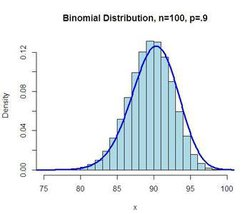
\includegraphics[width=0.7\textwidth]{BF.jpg}
	\caption{伯努利分布:来源于百度图片}
	\label{fig:digit}
\end{figure}
	
	而连续随机变量的累积概率分布与离散累积概率分布类似。连续随机变量的概率用\textbf{概率密度函数,probability density function}来概述。任何两点之间的概率密度函数所形成的区域就是该随机变量落在这两点之间的概率。概率密度函数可以简写为\textbf{p.d.f.,或者密度函数,或者密度}。
	\begin{figure}[htbp]
		\centering
		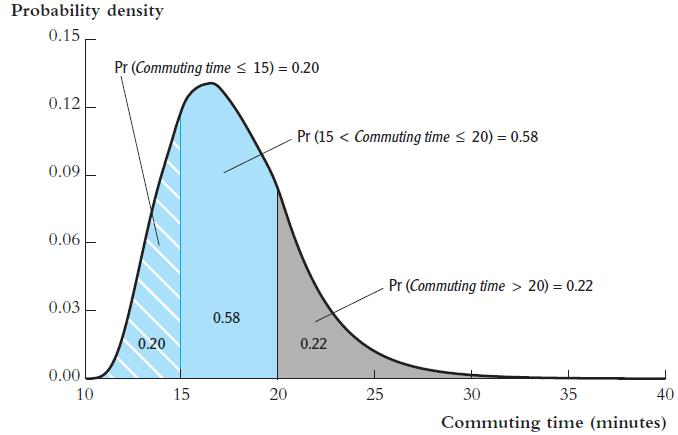
\includegraphics[width=0.7\textwidth]{pdf.jpg}
		\caption{概率密度函数:来源于Stock and Watson,2015,pp18}\label{fig:digit}
	\end{figure}
	
	\subsubsection{主要统计量}
	\textbf{期望}
	
	随机变量\emph{Y}的期望用\emph{E(Y)}表示,$\mu_{Y}$,指长期重复试验或发生的随机变量的均值。离散随机变量的期望是所有可能结果的加权平均,权数为每个结果发生的概率。
	
	例如,上面的电脑宕机次数的期望为:
	\begin{equation}
		\emph{E(M)}=0.8\times0+0.1\times1+0.06\times2+0.03\times3+0.01\times4=0.35
	\end{equation}
	
	也就是说,电脑宕机次数的期望为0.35次。需要注意的是,实际电脑宕机次数肯定是一个整数,我们说“写论文期间电脑宕机了0.35次”没有任何意义。而公式(1)的计算结果表明,写论文过程中,电脑宕机的平均次数。那么,随机变量的期望计算公式为
	\begin{equation}
		\emph{E(Y)}=p_1y_1+p_2y_2+\cdots+p_ky_k=\sum_{i=1}^{k}{p_iy_i}
	\end{equation}
	
	\textbf{标准差和方差}
	
	一个随机变量\emph{Y}的方差用$var(\emph{Y})$表示,其计算公式为$var(\emph{Y})=E\left[(Y-\mu_{Y})^2\right]$。
	
	而标准差是方差的开方,用$\sigma_{Y}$表示。
	\begin{equation}
		\sigma_{Y}^2=var(\emph{Y})=E\left[(Y-\mu_{Y})^2\right]=\sum_{i=1}^{k}{(y_i-\mu_{Y})^2p_i}
	\end{equation}
	
	根据公式(3),我们计算电脑宕机次数的方差和标准差为
	\begin{equation}
		var(\emph{Y})=0.8\times(0-0.35)^2+0.1\times(1-0.35)^2+0.06\times(2-0.35)^2+0.03\times(3-0.35)^2+0.01\times(4-0.35)^2=0.647
	\end{equation}
	\begin{equation}
		\sigma_{Y}=\sqrt{var(\emph{Y})}=\sqrt{0.647}\approx0.80
	\end{equation}
	
	\textbf{均值、方差的性质}
	
	(1)$Z=a+bY$,a,b都是常数,那么$E(Z)=E(a+bY)=a+bE(Y)$;
	
	(2)$var(Z)=var(a+bY)=b^2var(Y)$
	
	\textbf{其它分布特征}
	
	分布的特征除了均值和方差(或标准差)外,还有另外两个重要的形状指标:\textbf{峰度}—— 测量尾部有多“厚”,和\textbf{偏度}——测量分布非对称性程度。均值、方差、峰度和偏度都是分布的矩。
	
	一个随机变量Y的分布的峰度计算公式为
	\begin{equation}
		S(Y)=\frac{E\left[(Y-\mu_{Y})^4\right]}{\sigma_{Y}^4}
	\end{equation}
	
	偏度的计算公式为
	\begin{equation}
		S(Y)=\frac{E\left[(Y-\mu_{Y})^3\right]}{\sigma_{Y}^3}
	\end{equation}
	
	\subsection{多变量分布}
	大多数经济学问题都是以两个或多个随机变量的形式出现,例如,教育与工作收入、性别与工作收入等等。因此,我们必须了解多个随机变量的联合概率分布、边际概率分布和条件概率分布。
	
	\textbf{联合概率分布}
	
	两个离散随机变量($X,Y$)的联合概率分布就是两个随机变量同时取得某个值(例如,$x,y$)时的概率,其可以写成$Pr(X=x,Y=y)$。
	
	\textbf{边际概率分布}
	
	变量$Y$的边际概率分布仅仅只是Y概率分布的另一个名字,它是为了区分单一变量Y的分布和Y 与其他变量的联合概率分布。从联合概率分布中计算Y的边际概率分布,就是把Y 取某个特定值的所有概率相加。假设X取l个值,Y=y的边际概率分布为
	\begin{equation}
		Pr(Y=y)=\sum_{i=1}^{l}{Pr(X=x_i,Y=y)}
	\end{equation}
	
	\textbf{条件概率分布}
	
	给定X的值,随机变量Y的概率分布就叫做Y的条件概率分布,表示为$Pr(Y=y|X=x)$。条件概率分布的计算公式为:
	\begin{equation}
		Pr(Y=y|X=x)=\frac{Pr(X=x,Y=y)}{Pr(X=x)}
	\end{equation}
	
	\textbf{条件期望}
	
	给定X,Y的条件期望,也称为给定X,Y的条件均值,是给定X,Y的条件分布的均值。已知X=x条件下,Y的条件期望为
	\begin{equation}
		E(Y|X=x)=\sum_{i=1}^{k}{y_iPr(Y=y_i|X=x)}
	\end{equation}
	
	\textbf{期望迭代法则}
	
	Y的均值是给定X的条件下Y的条件期望的加权平均,而权重是X的概率分布。数学表达式为
	\begin{equation}
		E(Y)=\sum_{i=1}^{k}{E(Y|X=x_i)Pr(X=x_i)}
	\end{equation}
	
	换句话说,Y的期望就是给定X条件下,Y的期望的期望
	\begin{equation}
		E(Y)=E[E(Y|X)]
	\end{equation}
	
	公式(12)右边的内部期望是给定X条件下Y的条件期望,而外部期望是利用X的边际分布计算得到。而(12)就是期望迭代法则。
	
	需要注意的是,如果给定X条件下Y的条件期望为0,那么,Y的均值也为0。证明:$E(Y|X)=0$,$E(Y)=E[0]=0$,证毕。
	
	\textbf{条件方差}
	基于X的Y的条件方差是给定X的条件下Y的的概率分布的方差。公式为
	\begin{equation}
		var(Y|X=x)=\sum_{i=1}^{k}{[y_i-E(Y|X=x)]^2Pr(Y=y_i|X=x)}
	\end{equation}
	
	\textbf{相互独立}
	两个随机变量X和Y,如果在不提供一个随机变量的信息情况下,能得出另一个随机变量的值,那么,称X,Y独立分布,或者相互独立。尤其是,如果给定X的条件下Y的条件分布等于Y的边际分布,那么X,Y相互独立,即对于所有的x,y,如果
	\begin{equation}
		Pr(Y=y|X=x)=Pr{Y=y}
	\end{equation}
	那么,X和Y相互独立。
	
	把等式(14)代入公式(9)中,得到X和Y独立的另一个等价条件:\begin{equation}
		Pr(X=x,Y=y)=Pr(X=x)Pr(Y=y)
	\end{equation}
	
	也就是说,两个独立随机变量的联合分布就是它们的边际分布之积。
	
	\textbf{协方差和相关}
	\textbf{协方差}是测度两个随机变量共变程度的一种指标。通俗地说就是,你变,我也变,绝对值越大,说明我们两个越“心有灵犀”。X和Y的协方差是X与其均值之差乘以Y与其均值之差的期望,用$cov(X,Y)$表示。数学公式为
	\begin{equation}
		cov(X,Y)=\sigma_{XY}=E[(X-\mu_x)(Y-\mu_Y)]=\sum_{i=1}^{k}{\sum_{j=1}^{l}{(x_j-\mu_X)(y_i-\mu_Y)Pr(X=x_j,Y=y_i)}}
	\end{equation}
	
	如果两个随机变量同方向变动,那么,协方差为正;如果反方向变化,则协方差为负;如果相互独立,则协方差为0。
	
	由于协方差的单位为X的单位乘以Y的单位,因此,协方差的数值难以理解。为了解决“单位”问题,另一种表示X和Y之间相互依赖程度的测量指标就是\textbf{相关系数},即协方差除以标准差之积:
	\begin{equation}
		corr(X,Y)=\frac{cov(X,Y)}{\sqrt{var(X)var(Y)}}=\frac{\sigma_{XY}}{\sigma_X\sigma_Y}
	\end{equation}
	
	当$corr(X,Y)=0$,就说X和Y不相关。相关系数总是处于-1和1之间。
	
	如果Y的条件均值不依赖于X,那么,X和Y不相关。
	
	需要注意的是,独立,一定不相关;但不相关,不一定独立。
	
	分布特征的性质:
	
	(1)$E(X+Y)=E(X)+E(Y)=\mu_X+\mu_Y$
	
	(2)$var(X+Y)=var(X)+var(Y)+2cov(X,Y)=\sigma_{X}^2+\sigma_{Y}^2+2\sigma_{XY}$
	
	(3)$E(X^2)=\sigma_X^2+\mu_Y^2$
	
	(4)$E(XY)=\sigma_{XY}+\mu_X\mu_Y$
	
	\subsection{常用分布}
	计量经济学中最常用的概率分布是正态分布、卡方分布、t分布和F分布。
	
	\subsubsection{正态分布}
	正态分布的 连续随机变量有钟型概率密度形状,如图3所示。
		\begin{figure}[htbp]
		\centering
		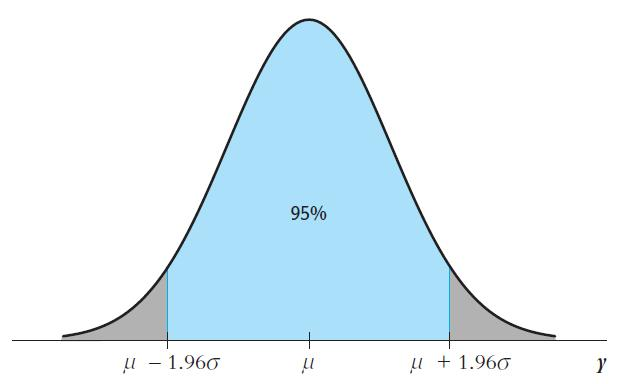
\includegraphics[width=0.7\textwidth]{normal.jpg}
		\caption{正态概率密度函数:来源于Stock and Watson,2015,pp36}\label{fig:digit}
	\end{figure}
	
	\textbf{数学定义:}一个连续随机变量$x_i$的概率密度函数为
	\begin{equation}
		f(x_i)=\frac{1}{\sqrt{2\pi\sigma^2}}e^{-\frac{1}{2\sigma^2}}(x_i-\mu)^2
	\end{equation}
	遵循正态分布,且均值为$\mu$,方差为$\sigma^2$。
	
	由上述数学定义可以看出,正态分布有两个参数,均值$\mu$,方差$\sigma$,因此,正态分布又可以表示为$N(\mu,\sigma^2)$。而其中,$\mu$又可以叫做尺度参数(scale parameter),$\sigma$称为形状参数(shape parameter)。 (注意:尺度参数和形状参数在后面的DSGE模型的贝叶斯估计中经常用到。大家知道有这些名称即可。)由此,可以定义\textbf{标准正态分布},即均值为0,方差为1的正态分布$N(0,1)$,通常用Z表示。标准正态积累分布方程用大写希腊字母表示$\Phi$,$Pr(Z\le{c})=\Phi(c)$。标准正态分布函数的图形如图4所示。
		\begin{figure}[htbp]
		\centering
		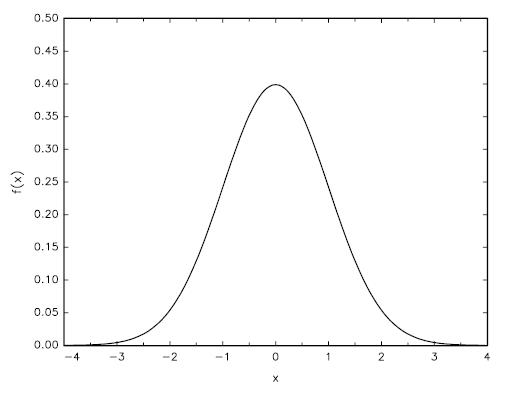
\includegraphics[width=0.7\textwidth]{snormal.jpg}
		\caption{标准正态分布函数:来源于Brown,2010}\label{fig:digit}
	\end{figure}
	

	
	从图3和图4中可以看到,正态分布的图形是在均值$\mu$处对称的。从图3中还可以看出,随机变量值落在均值附近$\pm2\sigma$区间内的概率为0.95。
	
	我在前面的1.1.2节给出了均值和方差的性质。这些内容也可以理解为随机变量的线性转换。即$x_i$是正态随机变量,那么它的线性变换$y_i$也是正态分布。且两个正态随机变量的线性组合仍然为正态分布。
	
	如果$x_i$是独立、同分布(iid)的正态随机变量,那么
	\begin{equation}
		\overline{x}_i~N(\mu_x,\frac{\sigma^2}{n})
	\end{equation}
	
	\textbf{任何一个正态随机变量都可以通过线性变换转换成标准正态随机变量。这一过程称为变量标准化。}这也为不同均值方差的正态分布的概率计算带来了方便。\textbf{变量标准化}就是随机变量减去均值,然后除以标准差。
	
	例1:假设$Y~N(1,4)$,求$Pr(Y\le2)$
	
	$\frac{(Y-1)}{\sqrt{4}}=\frac{1}{2}(Y-1)$
	
	$Y\le2$等价于$\frac{1}{2}(Y-1)\le{\frac{1}{2}(2-1)}$
	
	$Pr(Y\le2)=Pr[\frac{1}{2}(Y-1)\le{\frac{1}{2}}]=Pr(Z\le{\frac{1}{2}})=\Phi(0.5)=0.691$
	
	$\Phi(0.5)=0.691$可以从临界值表中查询。
	
	下面,我们来看看,正态分布变换成标准正态分布的正式数学过程:
	
	(1)首先,标准化
	
	$Z=\frac{\overline{x}-\mu_x}{\sqrt{\frac{\sigma_x^2}{n}}}=\frac{\overline{x}}{\sqrt{\frac{\sigma_x^2}{n}}}-\frac{\mu_x}{\sqrt{\frac{\sigma_x^2}{n}}}$
	
	
	
	(2)Z的均值
	
	$EZ=\frac{E\overline{x}}{\sqrt{\frac{\sigma_{x}^{2}}{n}}}-\frac{\mu_x}{\sqrt{\frac{\sigma_{x}^{2}}{n}}}=\frac{\mu_x}{\sqrt{\frac{\sigma_{x}^{2}}{n}}}-\frac{\mu_x}{\sqrt{\frac{\sigma_{x}^{2}}{n}}}=0$
	
	
	
	(3)Z的方差
	
	$Var(Z)=E(\frac{E\overline{x}}{\sqrt{\frac{\sigma_{x}^{2}}{n}}}-\frac{\mu_x}{\sqrt{\frac{\sigma_{x}^{2}}{n}}})^2=E[\frac{n}{\sigma_x^2}(\overline{x}-\mu_x)^2]=\frac{n}{\sigma_x^2}\frac{\sigma_x^2}{n}=1$
	
	正态分布在统计学中非常的重要。不仅是因为许多随机变量都遵循正态分布,而且更重要的是,任何样本随着其样本规模的增大,样本均值趋向于服从正态分布,这就是\textbf{中心极限定理}。
	
	\subsubsection{卡方分布}
	\textbf{卡方分布}是m个标准正态随机变量的平方和的分布,常用于检验某些类型的假设。其中,m称为自由度。例如,$Z_1$,$Z_2$,$Z_3$是标准正态随机变量,那么,$Z_1^2+Z_2^2+Z_3^2$就是一个自由度为3的卡方分布。一个自由度为m的卡方分布表示为:$\chi_m^2$。下面给出卡方分布的正式定义:
	
	\textbf{定义:}假设$Z_1$,$Z_2$,$Z_3$,$\cdots$,$Z_n$是一组简单的随机样本,且服从$Z_i~N(0,1)$,那么,
	\begin{equation}
		\sum_{i=1}^n{Z_i}~\chi_n^2
	\end{equation}
	其中,n为卡方分布的自由度。
	
	$\chi_n^2$的概率密度函数为
	\begin{equation}
		f_{\chi^2}(x)=\frac{1}{2^{\frac{n}{2}}\Gamma(\frac{n}{2})}x^{\frac{n}{2}-1}e^{\frac{-x}{2}},x\geq0
	\end{equation}
	
	其中,$\Gamma(x)$是伽马函数。如果任意一个服从正态分布的随机变量$x_i~N(\mu_x,\sigma_x^2)$,都有
	
	\begin{equation}
		\sum_{i=1}^n{(\frac{x_i-\mu}{\sigma})^2}~\chi_n^2
	\end{equation}
	
	卡方分布如图5所示。
		\begin{figure}[htbp]
		\centering
		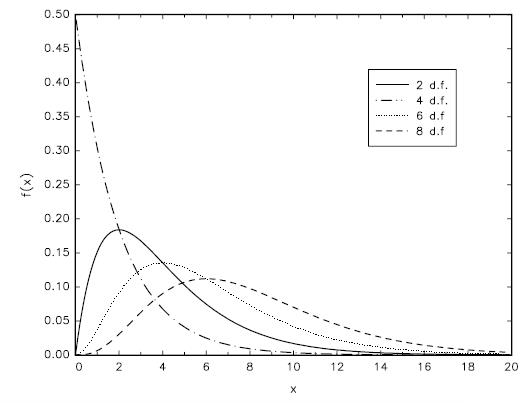
\includegraphics[width=0.7\textwidth]{chi.jpg}
		\caption{卡方分布函数:来源于Brown,2010}\label{fig:digit}
	\end{figure}
	

	
	\subsubsection{t分布}
	\textbf{t分布},也称为\textbf{学生t分布}是标准正态分布与自由度m的卡方分布除以m再开方的比率。用$t_m$表示。
	
	\textbf{定义:}假设$Z_i~N(0,1)$,$Y~\chi_m^2$,且Z和Y相互独立,那么,
	\begin{equation}
		\frac{Z}{\sqrt{\frac{Y}{m}}}~t_m
	\end{equation}
	其中,m为t分布的自由度。t分布的概率密度函数如图6所示。
		\begin{figure}[htbp]
		\centering
		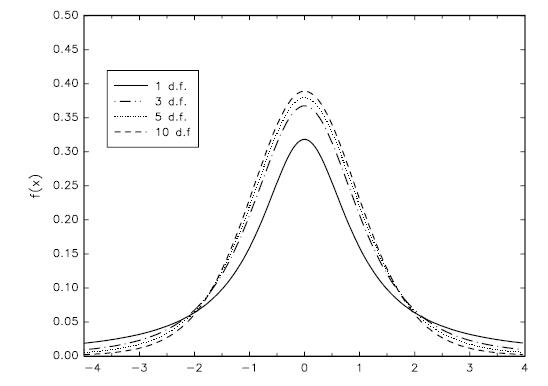
\includegraphics[width=0.7\textwidth]{t.jpg}
		\caption{t分布函数:来源于Brown,2010}\label{fig:digit}
	\end{figure}
	

	
	t分布也是钟型图案,类似于正态分布。但是当自由度较小(20或更小),更多落在尾部,也就说t分布比正态分布更扁平;当自由度大于等于30时,t分布近似于正态分布,而$t_{\infty}$ 等价于正态分布。
	
	\subsubsection{F分布}
	自由度为m,n的\textbf{F分布}\footnote{F分布是以伟大的统计学家Sir Ronald A. Fisher的名字命名的}是一个自由度为m的卡方随机变量除以m比上自由度为n的卡方随机变量除以n 的比值,表示为$F_{m,n}$。
	
	\textbf{定义:}假设$Y~\chi_m^2,W~\chi_n^2$,且Y和W相互独立,那么,
	\begin{equation}
		\frac{Y/m}{W/n}~F_{m,n}
	\end{equation}
	其中,m,n是F分布的自由度。
	
	注意:(1)如果x服从t分布,$x^2$服从F分布。(2)当分母的自由度趋向无穷时,$\frac{Y}{m}~F_{m,\infty}$。F分布的图形如图7所示。
	\begin{figure}[htbp]
	\centering
	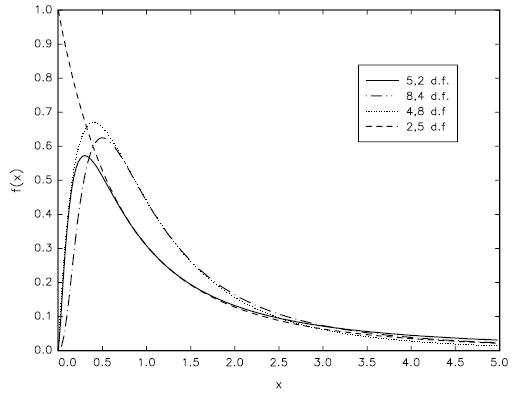
\includegraphics[width=0.7\textwidth]{F.jpg}
	\caption{F分布函数:来源于Brown,2010}\label{fig:digit}
\end{figure}


	
	\subsection{随机抽样与大样本近似}
	\subsubsection{随机抽样与样本矩}
	随机抽样就是从一个更大的总体中随机抽取一个样本。这个过程为了使样本均值(见1.3.1节)本身成为一个随机变量。那么,就可以探讨样本均值的分布——\textbf{抽样分布}。
	
	\textbf{简单随机抽样}是指从总体N个单位中任意抽取n个单位作为样本,使每个可能的样本被抽中的概率相等的一种抽样方式。
	
	因为$Y_1,Y_2,\cdots,Y_n$是从总体中随机抽取,因此,每一个样本$Y_i$的边际概率分布都相同,都与总体Y的分布相同。当$Y_i$有相同的边际概率分布时,我们称$Y_1,Y_2,\cdots,Y_n$ 为\textbf{同分布}。
	
	在简单随机抽样下,已知Y1的值并不能为Y2提供任何信息。因此,给定Y1条件下,Y2的条件概率分布与Y2的边际概率分布相同。也就是说,在简单随机抽样下,Y1的分布独立于Y2的分布。当$Y_1,Y_2,\cdots,Y_n$来自于相同的总体,又独立分布时,我们称为\textbf{独立同分布(i.i.d)}。
	
	考虑随机样本${Y_1,Y_2,\cdots,Y_n}$,假设$EY_i=\mu$,$Var(Y_i)=\sigma^2$。定义$S=Y_1+Y_2+\cdots+Y_n$为样本和。那么,
	\begin{equation}
		ES=E(Y_1+Y_2+\cdots+Y_n)=EY_1+EY_2+\cdots+EY_n=n\mu
	\end{equation}
	
	\begin{equation}
		Var(S)=E(S-ES)^2=E(Y_1+Y_2+\cdots+Y_n-n\mu)^2=E[\sum_{i=1}^n{(Y_i-\mu)}=n\sigma^2
	\end{equation}
	
	定义\textbf{样本均值}为$\overline{Y}=\frac{\sum_{Y_i}}{n}$。那么,
	\begin{equation}
		E\overline{Y}=E\frac{S}{n}=\frac{1}{n}ES=\frac{1}{n}n\mu=\mu
	\end{equation}
	
	\begin{equation}
		Var(\overline{Y})=E(\overline{Y}-\mu)^2=E(\frac{S}{n}-\mu)^2=frac{1}{n^2}E(S-n\mu)^2=\frac{\sigma^2}{n}
	\end{equation}
	
	\subsubsection{大样本近似}
	目前,有两种方法刻画抽样分布:精确法和近似法。
	
	精确分布又称有限抽样分布。
	
	“近似法”利用近似式来表达抽样分布,这种方法依赖于大样本规模。抽样分布的大样本近似通常称为\textbf{渐近分布}——“渐近”是因为随着n趋向于无穷,近似就变成精确了。
	
	注意:即使样本只有30个观测值,近似也非常精确。因为计量经济学中的观测值通常达到成百上千,因此,渐近分布能为精确抽样分布提供一个较好的近似。
	
	当样本很大的时候,两个法则很关键:大数法则和中心极限定理。
	
	\textbf{大数法则}是当样本规模很大时,$\overline{Y}$以很高的概率接近于$\mu_Y$。
	
	\textbf{中心极限定理}是当样本规模很大时,标准化样本均值的抽样分布,$\frac{(\overline{Y}-\mu_Y)}{\sigma_{\overline{Y}}}$,近似服从正太分布。
	
	因此,渐近正态分布并不依赖于Y的分布。渐近理论为回归分析提供了极大的简化。
	
	\subsection{小结}
	1、The probabilities with which a random variable takes on different values are summarized by the cumulative distribution function, the probability distribution function (for discrete random variables), and the probability density function (for continuous random variables).
	
	2、The expected value of a random variable Y (also called its mean, mY),denoted E(Y), is its probability-weighted average value. The variance of Y
	is $\sigma_Y^2=E[(Y-\mu_Y)^2]$, and the standard deviation of Y is the square root of its variance.
	
	3、The joint probabilities for two random variables X and Y are summarized by their joint probability distribution. The conditional probability distribution of Y given X = x is the probability distribution of Y, conditional on X taking on the value x.
	
	4、A normally distributed random variable has the bell-shaped probability density in Figure 4. To calculate a probability associated with a normal random variable, first standardize the variable and then use the standard normal cumulative distribution.
	
	5、Simple random sampling produces n random observations $Y_1,\cdots,Y_n$ that are independently and identically distributed (i.i.d.).
	
	6、The sample average, Y, varies from one randomly chosen sample to the next
	and thus is a random variable with a sampling distribution. If $Y_1,\cdots,Y_n$ are
	i.i.d., then:
	
	a. the sampling distribution of $\overline{Y}$ has mean $\mu_Y$ and variance $\sigma_{\overline{Y}}^2=\frac{\sigma_{Y}^2}{n}$;
	
	b. the law of large numbers says that $\overline{Y}$ converges in probability to $\mu_Y$; and
	
	c. the central limit theorem says that the standardized version of $\overline{Y}$,
	$\frac{(Y-\mu_Y)}{\sigma_{\overline{Y}}}$, has a standard normal distribution [N(0,1) distribution] when n is large.
	
	
	\section{统计学概述}
	\textbf{统计学}是应用数据来了解我们所生活世界的一门科学(Stock and Watson,2015)。统计工具能提供一些我们关注的总体分布特征。
	
	我们对整个世界,或者整个中国经济、社会、人口感兴趣。但是,以目前的技术水平,我们不可能去调查14人口,因为调查总体的成本非常大。但我们又想知道总体分布特征,怎么办?统计学的主要任务就是来解决这个问题。回忆一下,前一节讲过的随机抽样。我们只需要从总体中随机抽取样本,然后,利用统计方法,结合随机样本信息来推断总体分布特征。这样也可以得到一个较为满意的近似结果。
	
	计量经济学中使用的统计方法主要有三种:估计、假设检验与置信区间。\textbf{估计}就是从样本数据中,为一个总体分布特征——均值、方差等——计算出一个“最佳猜测”值。
	\textbf{假设检验}就是提出一个假设,然后用样本证据来验证假设是否为真。\textbf{置信区间}就是利用一组样本数据来估计未知总体分布特征的范围或区间。
	
	\subsection{估计}
	再次回忆一下随机抽样,从总体中随机抽取的样本$Y_1,\cdots,Y_n$是独立同分布(i.i.d.),且与总体Y同分布,那么,样本均值$\overline{Y}$就能很自然地被当作是总体均值$\mu_Y$。这种样本均值也称为总体均值的\textbf{估计量}\footnote{估计量(estimator)是数据样本的一个函数;估计(estimate)则是估计量的数值。}。
	
	但是,计算样本均值$\overline{Y}$是得到总体均值估计量的唯一一种方式吗?答案是否定的。$Y_1,\cdots,Y_n$都是与Y同分布,那么,$Y_1$也可以作为总体均值的一个估计量。以此类推,事实上,$\mu_Y$的估计量很多。那么,我们如何判断一个估计量比另一个估计量“更好”呢?我们前面讲过,抽样随机变量和样本均值都有概率分布,那么,这个问题还可以表达成:一个估计量的合意分布特征是什么呢?
	
	既然,我们是从样本信息中推断未知总体分布特征。那么,最合意的结果肯定是,样本估计量尽可能的接近总体分布“真值”。由此,可以给出,合意结果的三个特征:
	\textbf{无偏性}、\textbf{一致性}和\textbf{有效性}。注意,在后面的回归分析中,这三个特征非常非常重要。
	
	\textbf{无偏性}~~~如果你通过重复抽样来评估一个估计量,一般来说,你会得到一个“真值”。因此,一个估计量的合意性质就是要使其抽样分布均值等于总体均值$\mu_Y$。 如果是这样,那么,我们就称这个估计量\textbf{无偏}。用$\hat{\mu_y}$来表示$\mu_Y$的估计量。用$E(\hat{\mu_y})$表示估计量抽样分布的均值。如果$E(\hat{\mu_y})=\mu_Y$,那么,估计量$\hat{\mu_y}$是无偏的,反之亦然。
	
	\textbf{一致性}~~~当样本量很大时,由样本的随机变动引起的$\mu_Y$值的不确定性就非常小。也就是说,$\hat{\mu_y}$落入真值$\mu_Y$的一个较小区间内的概率随着样本量的增长而接近于1。即是说,$\hat{\mu_y}$是$\mu_Y$的一致估计。
	
	\textbf{有效性}~~~如果你有两个无偏的估计量$\hat{\mu_y}$和$\tilde{\mu_Y}$,那么,你会如何选择?此时,你应该选择最小方差的估计量。如果$\hat{\mu_y}$的方差比$\tilde{\mu_Y}$更小,就说明$\hat{\mu_y}$ 比$\tilde{\mu_Y}$更有效\footnote{“有效性”这这个术语源于,如果$\hat{\mu_y}$比$\tilde{\mu_Y}$方差更小,那么,$\hat{\mu_y}$能更有效的利用数据信息}。
	
	下面,我们来看看样本均值$\overline{Y}$是否满足上述估计量的三个标准。
	
	(1)样本均值等于总体均值已经在1.4.1节证明$\overline{Y}=\mu$,因此,样本均值是无偏的。
	
	(2)根据大数法则,见1.4.2节,样本规模越大,$\overline{Y}$以很大概率接近$\mu$,因此,样本均值是一致的。
	
	(3)那怎么判断$\overline{Y}$是有效的估计量呢?回忆一下,我在前面提到过,$\mu_Y$的估计量还有很多,例如$Y_1,Y_2,\cdots,Y_n$。我们现在选择用$Y_1$与$\overline{Y}$进行比较。首先,$Y_1$与$\overline{Y}$都是无偏估计。而$Y_1$的方差为$Var(Y_1)=\sigma_Y^2$。 根据1.4.1节,$\overline{Y}$的方差为$\frac{\sigma_Y^2}{n}$。只要$n\ge2$,那么,$\overline{Y}$的方差就小于$Y_1$的方差,因此,$\overline{Y}$是有效估计量。
	
	综上所述,我们也把样本均值$\overline{Y}$称为最优线性无偏估计(\textbf{B}est \textbf{L}inear \textbf{U}nbiased \textbf{E}estimator,\textbf{BLUE})。
	
	此外,还有一点非常重要,那就是随机抽样的重要性。虽然我们不能实施一个完全随机的抽样,但是我们设计的抽样要尽可能降低偏误。
	
	\subsection{假设检验}
	待检验的假设成为\textbf{原假设}。假设检验就是用数据来比较原假设与另一个假设——\textbf{备择假设}。如果原假设不成立,那么,备择假设成立。在统计学中,原假设通常为总体均值等于某一特定值,用$H_0$表示,即
	\begin{equation}
		H_0:E(Y)=\mu_{Y,0}
	\end{equation}
	
	最常用的备择假设为$H_1:E(Y)\neq\mu_{Y,0}$,这种类型被称为\textbf{双向备择假设},因为该假设允许$E(Y)$要么大于特定值,要么小于特定值。
	
	统计学理论将会告诉我们如何利用样本数据来判断是否接受$H_0$,还是接受$H_1$。
	
	现实中,我们不可能知道总体均值,只能用随机抽样的样本均值$\overline{Y}$代替。那么,$\overline{Y}$不可能精确地等于$\mu_{Y,0}$。$\overline{Y}$与$\mu_{Y,0}$之间的差异,要么是因为真实均值并不等于$\mu_{Y,0}$(原假设为假),要么因为真实均值等于$\mu_{Y,0}$ (原假设为真)但由于随机抽样使得$\overline{Y}$与$\mu_{Y,0}$ 不等。这两种可能性,几乎区分不了,但我们可以计算一个概率来允许检验原假设。即利用数据来计算原假设的p值。
	
	\textbf{p值,也称为显著性概率}是利用样本数据计算的一个对原假设不利的概率值。也就是说,p值越小,结果越显著。其数学定义为
	\begin{equation}
		p-value=Pr[|\overline{Y}-\mu_{Y,0}|\geq|\overline{Y}^{act}-\mu_{Y,0}|]
	\end{equation}
	其中,$\overline{Y}^{act}$表示用实际数据计算的样本均值,$Pr_{H_0}$原假设下计算的概率。也就是说,p值是$\overline{Y}$的分布尾部超出$\mu_{Y,0}\pm|\overline{Y}^{act}-\mu_{Y,0}|$的区域。如果p值越大,观测到的$\overline{Y}^{act}$就与原假设一致,如果p较小,则拒绝原假设。
	\begin{figure}[htbp]
		\centering
		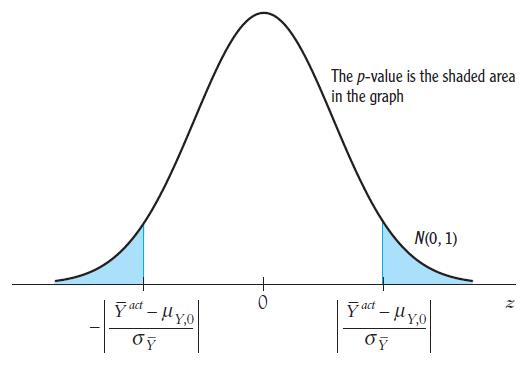
\includegraphics[width=0.7\textwidth]{p.jpg}
		\caption{p值:来源于Stock and Watson,2015,pp74}\label{fig:digit}
	\end{figure}
	
	\textbf{t统计量}
	
	\begin{equation}
		t=\frac{\overline{Y}-\mu{Y,0}}{SE(\overline{Y})}
	\end{equation}
	
	当样本规模很大时,t的分布近似于标准正态分布$N(0,1)$
	
	在假设检验中通常犯两类错误:(1)\textbf{第一类错误},原假设为真时却被拒绝;(2)\textbf{第二类错误},原假设为假时却没有拒绝。
	
	如果你选择拒绝原假设(为真)的预设概率水平(例如,5\%),那么,只有p 值小于0.05时才拒绝原假设。在实践中,5\%对应的标准正态分布的尾部区域是$\pm1.96$之外的区域,即简单规则为
	\begin{equation}
		如果|t^{act}|\geq1.96,拒绝H_0
	\end{equation}
	
	也就是说,第一类错误的预设概率就是检验的\textbf{显著性水平}。
	
	实践中,常用的显著性水平有:10\%、5\%、1\%、0.1\%。
	
	\subsection{置信区间}
	
	总体均值的95\%置信区间就是真值有95\%的概率落入该区间。当样本规模很大时,90\%、95\%、99\%对应的置信区间为
	\begin{center}
		$90\%:\mu_Y=[\overline{Y}\pm{1.64E(\overline{Y})}]$\\
		$95\%:\mu_Y=[\overline{Y}\pm{1.96E(\overline{Y})}]$\\
		$99\%:\mu_Y=[\overline{Y}\pm{2.58E(\overline{Y})}]$
	\end{center}
	
	\section{贝叶斯统计概述}
	贝叶斯(T. Bayes,1702-1763)是英国数学家。他首先将归纳推理法用于概率论基础理论,并创立了贝叶斯统计理论,对于统计决策函数、统计推断、统计估算等作出了重要贡献。
	
	贝叶斯于1763年在英国皇家学会学报上发表“An essay towards solving a problem in the doctrine of chances"。该文中提出的二项分布参数推断方法后来被称为贝叶斯定理。贝叶斯公式
	\begin{equation}
		P(A|B)=\frac{P(A)P(B|A)}{P(B|A)P(A)+P(B|A^c)P(A^c)}
	\end{equation}
	
	看上去贝叶斯公式只是把 A 的后验概率转换成了 B 的后验概率 + A 的边缘概率的组合表达形式,因为很多现实问题中$P(A|B)$很难直接观测,但是$P(B|A)$和$P(A)$却很容易测得,利用贝叶斯公式可以方便我们计算很多实际的概率问题。
	
	具体可以参见:
	
	(1)朱慧明,林静. 2009,《贝叶斯计量经济模型》,科学出版社
	
	(2)Koop, G., Poirier, D. J.,  Tobias, J. L. (2007). Bayesian econometric methods. Cambridge University Press.
	
	(3)Geweke, J. (2005). Contemporary Bayesian econometrics and statistics (Vol. 537). John Wiley and Sons.
	
	(4)Koop, G.,  Korobilis, D. (2010). Bayesian multivariate time series methods for empirical macroeconomics. Foundations and Trends? in Econometrics, 3(4), 267-358.
	
	
	
	\section{附录}
	
	
	
	\chapter{一元线性回归}
	
	2015年,政府提高香烟消费税对吸烟率的影响是什么?小班教学能提高学生测试得分吗?性别对工资的影响是什么?
	
	其实,上述三个问题都是在问一个变量,X(包括消费税、班级规模和性别)的变化对另一个变量,Y (包括吸烟率、测试分数和工资)的影响。
	
	线性回归模型就是把X和Y联系起来。这条回归线的斜率就是X变化一单位引起的Y的变化。因为Y 的总体均值未知,所以这个斜率也未知。而计量经济学就是要用X,Y的样本数据来估计回归线的斜率。
	\section{线性回归模型估计}
	\subsection{线性回归模型}
	回顾一下小班教学的例子。李院长还不太确定是否要缩减你们本科的班级规模。假设你们是计量经济学家或者咨询师,李院长来向你们寻求帮助。李院长说,他面临着一个选择困难:一方面,父母肯定是希望小班教学;另一方面,缩小班级规模,就要雇佣更多的老师,要支出更多的经费。因此,他问你们:如果缩小班级规模,学生的成绩会发生什么变化?
	
	也就是说,如果李院长要改变班级规模,例如每个班级缩减10名学生,那么,学生的标准化成绩会发生什么变化?我们用希腊字母,$\beta_{ClassSize}$,来表示班级规模变化引起的成绩变化,数学表达式为
	\begin{equation}
		\beta_{ClassSize}=\frac{Score Change}{Classsize Change}=\frac{\Delta{Score}}{\Delta{ClassSize}}
	\end{equation}
	
	其中,$\Delta$表示变化量;而$\beta_{ClassSize}$就是由班级规模变化引起的学生成绩变化与班级规模变化的比值。如果你们运气好,知道了这个$\beta_{ClassSize}$,例如,-0.5,那么,你们可以直接告诉李院长,班级规模变小,会让学生的成绩提高,且根据公式(1),提高的幅度为:
	\begin{equation}
		\Delta{Score}=\beta_{ClassSize}\times\Delta{ClassSize}
	\end{equation}
	
	那么,班级规模减少10名学生,预期学生成绩会提高$(-0.5)\times(-10)=5$。 也就说,每个班级减少10名学生,预期学生成绩会提高5分。据此,公式(1)定义了班级规模与学生成绩之间直线的斜率。因此,可以把这条直线写成
	\begin{equation}
		Score=\beta_0+\beta_{ClassSize}\times{ClassSize}
	\end{equation}
	
	这个时候,你会不会兴奋地拿着公式(3)跑到李院长办公室,告诉他,我不仅能告诉您每个班级减少10人,学生成绩会提高多少。而且,只要您告诉我班级规模,我还能预期到学生的平均成绩会是多少。但是,李院长会说,不好意思,我对你这个方程和结果表示怀疑。因为每个班的学生本身有差异,每个班的授课老师不同,可能用的课本也不同。这些原因都可能导致学生的成绩不同,因此,公式(3)并不是对所有班级都成立。
	
	接受了李院长的建议,回去重新修正模型,加入影响学生成绩的其他因素,得到下式
	\begin{equation}
		Score=\beta_0+\beta_{ClassSize}\times{ClassSize}+OtherFactors
	\end{equation}
	
	其中,$OtherFactors$里面包含了李院长提到的,和没提到的影响学生成绩的因素。公式(4)更一般化,因为我们关注于班级规模与学生成绩,所以才能把其它因素统统“装进”$OtherFactors$中。假设有n个班级,$Y_i$表示第i个班级的平均成绩,$X_i$ 表示第i个班级的学生人数。那么,公式(4)就可以表示为
	\begin{equation}
		Y_i=\beta_0+\beta_1X_i+u_i
	\end{equation}
	
	公式(5)称为\textbf{一元线性回归模型},Y称为\textbf{因变量或被解释变量},X 称为\textbf{自变量或解释变量}。$\beta_0+\beta_1X_i$称为\textbf{总体回归线或总体回归方程}。截距$\beta_0$和斜率$\beta_1$是总体回归线的系数,也称参数。斜率$\beta_1$可以理解为X变化一单位,Y的变化程度。\footnote{需要注意的是,从数学上理解,截距$\beta_0$是X=0时Y的值,也就是总体回归线与Y轴的交点。但在经济学忠,这个截距有时候有经济学含义,有时候则没有经济学含义,例如班级规模为0 时,班级的平均成绩为$\beta_0$就不符合实际了,因此,这个时候要将其单纯理解成数学意义上的系数。}
	
	$u_i$为\textbf{误差项},其对应着第i个班级平均成绩与总体回归线预测的成绩只检测差异的所有因素。因此,误差项包含除了X之外所有决定因变量Y的因素。
	
	\subsection{系数估计}
	在实际情形中,我们不可能知道总体分布,即我们不可能知道总体回归线中的两个参数值。但是从第二讲可知,我们可以从随机抽样的样本数据中估计总体参数。同理,我们也可以用数据来估计总体回归线的斜率与截距。
	
	如果大家有兴趣,可以去调查一下班级大小与成绩的信息,然后自己估计一下回归系数。正如第一讲中提到,这类调查往往成本巨大,可能有一些机构或者教育部门有这类调查数据,但是很遗憾没有公开。那么,我们就暂且使用一下美帝的数据样本来作为例子。数据为1999年加利福利亚420个学区的测试分数和班级规模。表1中概述了这两个样本的分布。
	\begin{table}[htbp]
		\caption{测试分数与师生比的分布}\label{tab:digit}
		\centering
		\begin{tabular}{lcccccc}
			\hline
			&&&&\multicolumn{3}{c}{分位数}\\
			\cline{5-7}
			&样本量&均值&标准差&10\%&50\%&95\%\\
			\cline{1-7}
			学生-老师比&420&19.64&1.89&17.35&19.72&22.65\\
			\cline{1-7}
			测试分数&420&654.16&19.05&630.38&654.45&685.5\\
			\hline
		\end{tabular}
	\end{table}
	
	由表1可以看到,平均每个老师带19.64个学生,标准差为1.89。每个学区的分数均值为654.16,标准差为19.05。两个样本的散点图,如图1所示。分数与班级规模的相关系数为-0.226。
	\begin{figure}[htbp]
		\centering
		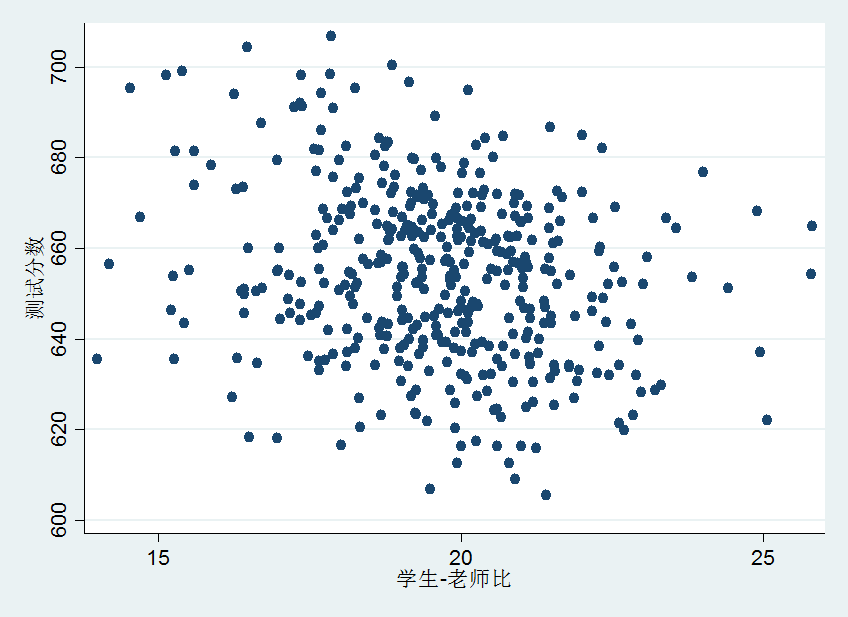
\includegraphics[width=0.7\textwidth]{score.png}
		\caption{学生-老师比与分数散点图}\label{fig:digit}
	\end{figure}
	
	根据散点图和相关系数,我们大致可以判断基于这些数据的直线应该是向右下倾斜。只要我们画出这条线,我们就得到了斜率$\beta_1$的估计值。但是我们如何画出这条线呢?最常用的方法就是普通最小二乘(OLS)来拟合这些数据。
	
	(1)\textbf{OLS估计量}
	OLS估计量使得估计的回归线尽量的接近观测数据。而接近程度则由给定X条件下,预测Y的误差平方和来测度。
	
	假设$\hat\beta{_0}$和$\hat\beta{_1}$用来表示$\beta_0$和$\beta_1$的估计量。那么,第i 个观测值的误差为$Y_i-\beta_0-\beta_1X_i$。那么,误差平方和为
	\begin{equation}
		\sum_{i=1}^n{(Y_i-\beta_0-\beta_1X_i)^2}
	\end{equation}
	
	根据第二讲的统计学理论,存在唯一一对$\hat\beta{_0}$和$\hat\beta{_1}$ 来使得公式(6)最小化。由此得到的系数为$\beta_0$和$\beta_1$的OLS估计量。OLS回归线称为样本回归线或样本回归函数。第i个观测值$Y_i$与其预测值之差为余项(residual):$\hat{u}_i=Y_i-\hat{Y}_i$。
	
	OLS估计量的公式为
	\begin{equation}
		\hat\beta{_1}=\frac{\sum_{i=1}^n{(X_i-\overline{X})(Y_i-\overline{Y})}}{\sum_{i=1}^n{(X_i-\overline{X})^2}}
	\end{equation}
	\begin{equation}
		\hat\beta{_0}=\overline{Y}-\hat\beta{_1}\overline{X}
	\end{equation}
	
	OLS预测值及残差
	\begin{equation}
		\hat{Y}_i=\hat\beta{_0}+\hat\beta{_1}X_i
	\end{equation}
	\begin{equation}
		\hat{u}_i=Y_i-\hat{Y}_i
	\end{equation}
	
	(2)\textbf{示例}
	我们用Stata14来估计OLS回归线:
	\begin{equation}
		\hat{Y}=698.9-2.28\times{X}
	\end{equation}
	\begin{figure}[htbp]
		\centering
		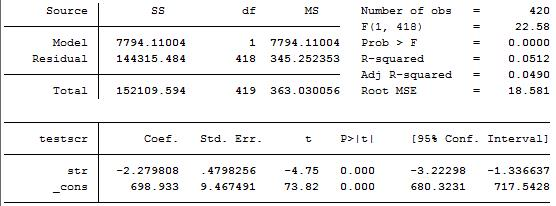
\includegraphics[width=0.7\textwidth]{stata1.jpg}
		\caption{stata结果}\label{fig:digit}
	\end{figure}
	
	我们在Y上面加hat是为了区别它为基于OLS回归线的预测值。负斜率意味着班级规模越大,平均测试分数越低。
	\subsection{拟合度}
	我们已经估计出了班级规模对测试成绩效应的线性回归,如公式(11)。正如李院长质疑的,我们都可能疑惑,估计的线性回归线对数据的拟合程度如何呢?
	
	在计量经济学中,$R^2$和回归标准误(SER)用来测量OLS回归线对数据的拟合程度。$0\leq{R^2}\leq1$测量的是$X_i$能解释$Y_i$的方差的比例。SER测量的是$Y_i$ 离预测值有多远。
	
	(1)\textbf{$R^2$}
	
	根据预测值与残差的定义,可知
	\begin{equation}
		Y_i=\hat{Y}_i+\hat{u}_i
	\end{equation}
	
	根据$R^2$的定义,它的数学形式可以表达为\textbf{回归平方和或者解释平方和}(\textbf{explained sum of squares,ESS})与\textbf{总平方和}(\textbf{Total Sum of Squares,TSS})之比。
	\begin{equation}
		ESS=\sum_{i=1}^n{(\hat{Y}_i-\overline{Y})^2}
	\end{equation}
	\begin{equation}
		TSS=\sum_{i=1}^n{(Y_i-\overline{Y})^2}
	\end{equation}
	那么,$R^2$的公式为
	\begin{equation}
		R^2=\frac{ESS}{TSS}
	\end{equation}
	
	我们还可以这么思考:X不能解释Y的方差的比例,同样可以表示出$R^2$。不能解释的部分就是\textbf{残差平方和(sum of squared residuals,SSR)},即$SSR=\sum_{i=1}^n{\hat{u}_i^2}$。综上所述,$TSS=ESS+SSR$。据此,
	\begin{equation}
		R^2=1-\frac{SSR}{TSS}
	\end{equation}
	
	注:一元回归中的$R^2$就是X和Y的相关系数的平方。$R^2$越接近于1,说明用X预测Y越好,即回归线拟合数据越好,反之亦然。
	
	\textbf{SER}
	
	回归标准误(SER)是回归误差标准差的估计量。它是观测值在回归线附近的分散程度的一种测量。OLS残差为$\hat{u}_i$。那么,
	\begin{equation}
		SER=\sqrt{S_{\hat{u}}^2},S_{\hat{u}}^2=\frac{1}{(n-2)}\sum_{i=1}^{n}{\hat{u}_i^2}=\frac{SSR}{(n-2)}
	\end{equation}
	
	其中,OLS残差的样本均值为0。
	
	例如,图2中的回归结果,$R^2=0.0512,SER(MSE)=18.581$。这意味着,班级规模可以解释测试分数方差的5.21\%。而$SER=18.581$说明观测值在回归线附近分散较开,这也可以从图3中看出。
	\begin{figure}[htbp]
		\centering
		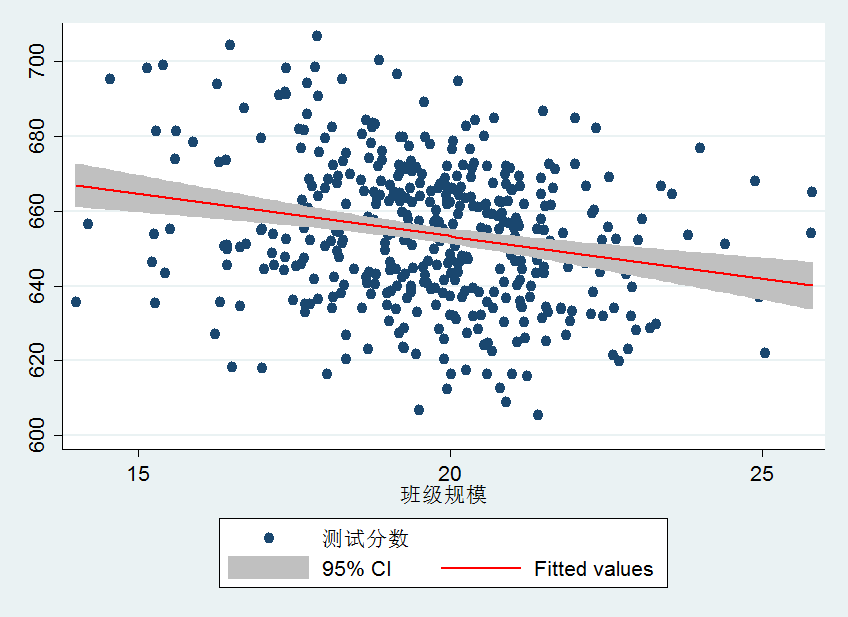
\includegraphics[width=0.7\textwidth]{Rline.png}
		\caption{回归线}\label{fig:digit}
	\end{figure}
	
	注意:\textbf{事实上,$R^2$很小(或者$SER$很大)本身并不能说明回归的“好坏”。很小的$R^2$只是表面,除了解释变量X外,还有其它重要的因素影响Y。但是较小的$R^2$ 或者较大的$SER$并不能给出缺失的重要因素是什么,它们仅仅说明现有的X只能解释Y方差的较小部分。}
	
	\subsection{最小二乘的假设}
	下面,我们简单的介绍一下OLS的三个假设。
	
	\textbf{假设一:给定X的条件下,u的条件均值为0}
	
	这个假设是说,“丢弃”到残差项u里的其它因素与X无关,即给定X条件下,这些因素的分布均值为0。该假设等价于总体回归线就是给定X条件下的Y的条件均值。且该假设也意味着$corr(X,u)=0$。
	
	\textbf{假设二:($X_i,Y_i$)是独立同分布}
	
	\textbf{假设三:$X_i,Y_i$不可能有较大奇异值}
	
	较大的奇异值会使得OLS结果产生误差。这个假设就使得X,Y有非零的四阶矩:$0\leq{E(X_i^4)}\leq\infty$,$0\leq{E(Y_i^4)}\leq\infty$。也就说,X和Y 存在有限峰度。可能的来源:1、输入错误;2、单位错误。如果输入错误,就纠正它,如果不能纠正,就从样本中删除。
	
	\section{假设检验和置信区间}
	第一部分概述了一元回归系数的估计,这个部分将概述估计量有多精确地描述了抽样不确定性。
	
	\subsection{回归系数的假设检验}
	有一些人武断地说,班级规模并不会对测试分数产生影响。也就说,总体回归线的斜率$\beta{_1}=0$。下面,我们就来检验斜率是否为0。也就说,我们先假设$\beta{_1}=0$ (原假设)。然后,我们来判断是否接受或者拒绝原假设。
	
	首先,我们回顾一下3.2节中的总体假设检验。
	
	原假设为Y的均值为某一特定值$\mu_{Y,0}$,可以写成$H_0:E(Y)=\mu_{Y,0},H_1\neq\mu_{Y,0}$。
	
	假设检验分三步走:
	
	1、计算$\overline{Y}$的标准误$SE(\overline{Y})$;
	
	2、计算t统计量,即$t=\frac{(\overline{Y}-\mu_{Y,0})}{SE(\overline{Y})}$;
	
	3、计算p值,它是拒绝原假设的最低显著性水平。双边假设p值为$2\Phi{(-|t_{act}|)}$,其中,$t_{act}$是计算得到的t统计量,$\Phi$是积累标准正态分布。
	
	在实践中,第三步的p值通常与临界值比较。例如,5\%显著性水平的双边假设对应着$|t_{act}|>1.96$。即是说,总体均值在5\%的显著性水平下显著异于假设值。
	
	\textbf{系数的假设检验}
	
	上面已经提到过,有些人觉得小班没有效果。我们应该假设$\beta_1=0$,那么,原假设和双边备择假设为
	\begin{equation}
		H_0:\beta_1=0~~vs.~~H_1\neq0
	\end{equation}
	
	那么,按照上述三步走:
	
	第一步:计算$\hat{\beta}_1$的标准误$SE(\hat{\beta}_1)$。该标准误是$\sigma_{\hat{\beta}_1}$的一个估计值。即
	\begin{equation}
		SE(\hat{\beta}_1)=\sqrt{\hat{\sigma}_{\hat{\beta}_1}^2}
	\end{equation}
	
	其中,
	\begin{equation}
		\hat{\sigma}_{\hat{\beta}_1}^2=\frac{1}{n}\times\frac{\frac{1}{n-2}\sum_{i=1}^n{(X_i-\overline{X})^2\hat{u}_i^2}}{[\frac{1}{n}\sum_{i=1}^n{(X_i-\overline{X})^2}]^2}
	\end{equation}
	
	第二步:计算t统计量
	\begin{equation}
		t=\frac{\hat{\beta}_1-0}{SE(\hat{\beta}_1)}
	\end{equation}
	
	第三步:计算p值
	\begin{multline}
		p-value=Pr_{H_0}[|\hat{\beta}_1-0|>|\hat{\beta}_1^{act}-0|]\\
		=Pr_{H_0}[|\frac{\hat{\beta}_1-0}{SE(\hat{\beta}_1)}|>|\frac{\hat{\beta}_1^{act}-0}{SE(\hat{\beta}_1)}|]=Pr_{H_0}(|t|\geq|t^{act}|)
	\end{multline}
	
	因为t统计量近似标准正态分布,因此
	\begin{equation}
		p-value=Pr(|Z|>|t^{act}|)=2\Phi(-|t^{act}|)
	\end{equation}
	
	如果p值小于5\%,即是说,在5\%的显著性水平下拒绝原假设。5\%的显著性水平对应着1.96的临界值。
	
	在实践中,我们并不用分别按照上述步骤计算出估计量和统计量,因为现在我们有计量经济学软件包,例如Stata。我们把数据导入stata中,输入回归命令就可以直接得到上述三个步骤的结果,如图2所示。
	
	例如,从图2中可以看出,$\beta_1$的标准误为0.48,系数为-2.28,那么$t=\frac{-2.28-0}{0.48}=-4.75$。t统计量的绝对值大于1.96,也就是在5\% 显著性水平下拒绝原假设。其实,我们计算的t统计量绝对值还要大于2.58 (1\%)。
	
	\subsection{置信区间}
	从样本数据并不能得到系数的真值。但是,我们能根据OLS估计量和标准误构建一个包含真值的置信区间。
	
	系数$\beta_1$的95\%置信区间:
	
	1、用5\%显著性水平的双边假设检验不能拒绝的一系列值;
	
	2、有95\%的可能性包含$\beta_1$真值的区间
	
	当样本规模很大时,$\beta_1$的95\%置信区间为
	\begin{equation}
		[\hat{\beta}_1-1.96SE(\hat{\beta}_1),\hat{\beta}_1+1.96SE(\hat{\beta}_1)]
	\end{equation}
	
	例如,班级规模与测试分数回归中的$\beta_1$的95\%置信区间为$[-2.28\pm1.96\times0.48]=[-3.22,-1.34]$
	
	\subsection{虚拟变量}
	迄今为止,我们讨论的自变量为连续型变量。还有一类回归因子为二值,即它只取两个值——0和1。例如,当班级规模小于20人时为小班,X取值为1,当班级规模大于等于20人时为大班,X取值为0。这样的变量也被称为\textbf{指示变量、哑变量或虚拟变量}。
	
	虚拟变量回归与上述回归相同,但是对于虚拟变量回归系数的理解却有些不同。
	
	二值因变量回归实际上就是执行了一个均值差分。假设$D_i$等于0或1,取决于班级规模大小:
	\[ D_i=\begin{cases}
		1,\quad X<20 \\
		0,\quad X\geq20
	\end{cases} \]
	
	总体回归方程为
	\begin{equation}
		Y_i=\beta_0+\beta_1D_i+u_i
	\end{equation}
	
	因为$D_i$是二值,那么,不能再将$\beta_1$理解成斜率,因为回归方程不是一条线了。那么,我们应该如何理解$D_i$呢?当$D_i=0$时,回归方程变成
	\begin{equation}
		Y_i=\beta_0+u_i
	\end{equation}
	
	因为$E(u_i|D_i)=0$,所以$E(Y_i|D_i=0)=\beta_0$。也就是说,$\beta_0$是大班的情况下的平均分数。类似地,当$D_i=1$时,回归方程变成
	\begin{equation}
		Y_i=\beta_0+\beta_1+u_i
	\end{equation}
	
	因此,$E(Y_i|D_i=1)=\beta_0+\beta_1$;即是说$\beta_0+\beta_1$是小班的平均分。
	
	综上所述,$(\beta_0+\beta_1)-\beta_0=\beta_1$就是小班和大班平均分数的差异。换句话说,$\beta_1=E(Y_i|D_i=1)-E(Y_i|D_i=0)$。因为$\beta_1$是总体均值之间的差异,因此,OLS估计量就是两个组的Y的平均值之差。
	
	假设检验和置信区间与前面内容相同。
	
	例如,小班教学的例子中,设置学生-老师比小于20时虚拟变量为1,其余为0。 回归结果如下图所示。
	\begin{figure}[htbp]
		\centering
		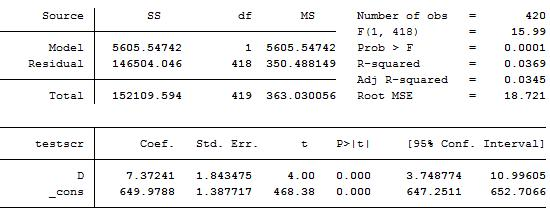
\includegraphics[width=0.7\textwidth]{dummy.jpg}
		\caption{虚拟变量回归结果}\label{fig:digit}
	\end{figure}
	
	
	\section{STATA教程(一)}
	Stata是一款流行的统计软件包。目前已经更新至stata15,更多详细信息可参见\url{www.stata.com}。本讲稿向大家介绍Stata以及上述回归的操作。
	
	我使用的Stata14 MP版。点击桌面的“stata”图标,打开之后的界面如下图
	\begin{figure}[htbp]
		\centering
		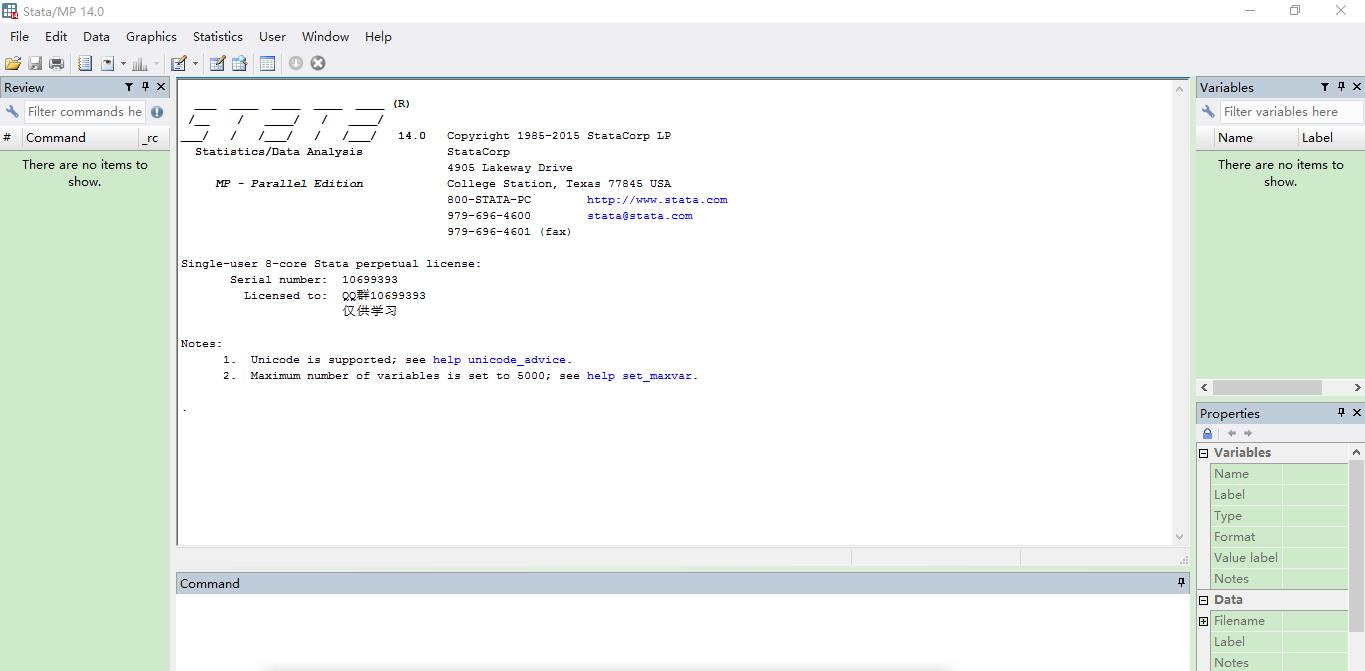
\includegraphics[width=1\textwidth]{stata.jpg}
		\caption{stata界面}\label{fig:digit}
	\end{figure}
	
	stata面板最上面是“菜单栏”
	
	左边窗口是“历史命令”
	
	中间上窗口是“结果显示”
	
	中间下窗口是“命令”
	
	右边上窗口是“变量名”
	
	(1)数据输入
	
	首先点击“菜单栏”中的“Data”—“Data Editor”,选择“Data Editor(Edit)”,就会出现如下窗口
	\begin{figure}[htbp]
		\centering
		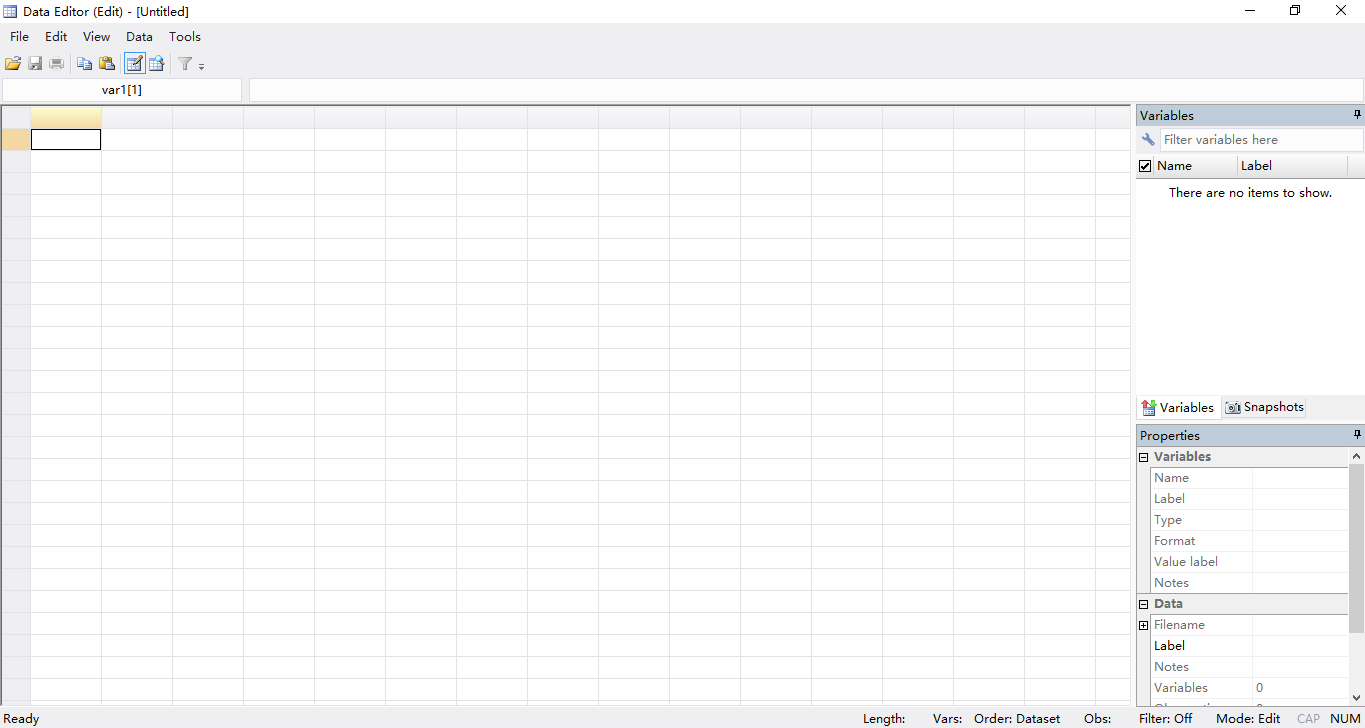
\includegraphics[width=1\textwidth]{data edit.png}
		\caption{数据输入界面}\label{fig:digit}
	\end{figure}
	
	在这个界面,我们可以手动输入数据,也可以直接从Excel中复制粘贴。我们输入的数据如下:
	\begin{table}[htbp]
		\caption{输入数据}\label{tab:digit}
		\centering
		\begin{tabular}{ccc}
			\hline
			obs&testscr&str\\
			1&690.8&17.889\\
			2&661.2&21.5247\\
			3&643.6&18.6713\\
			\vdots&\vdots&\vdots\\
			\hline
		\end{tabular}
	\end{table}
	
	得到如下界面:
	\begin{figure}[htbp]
		\centering
		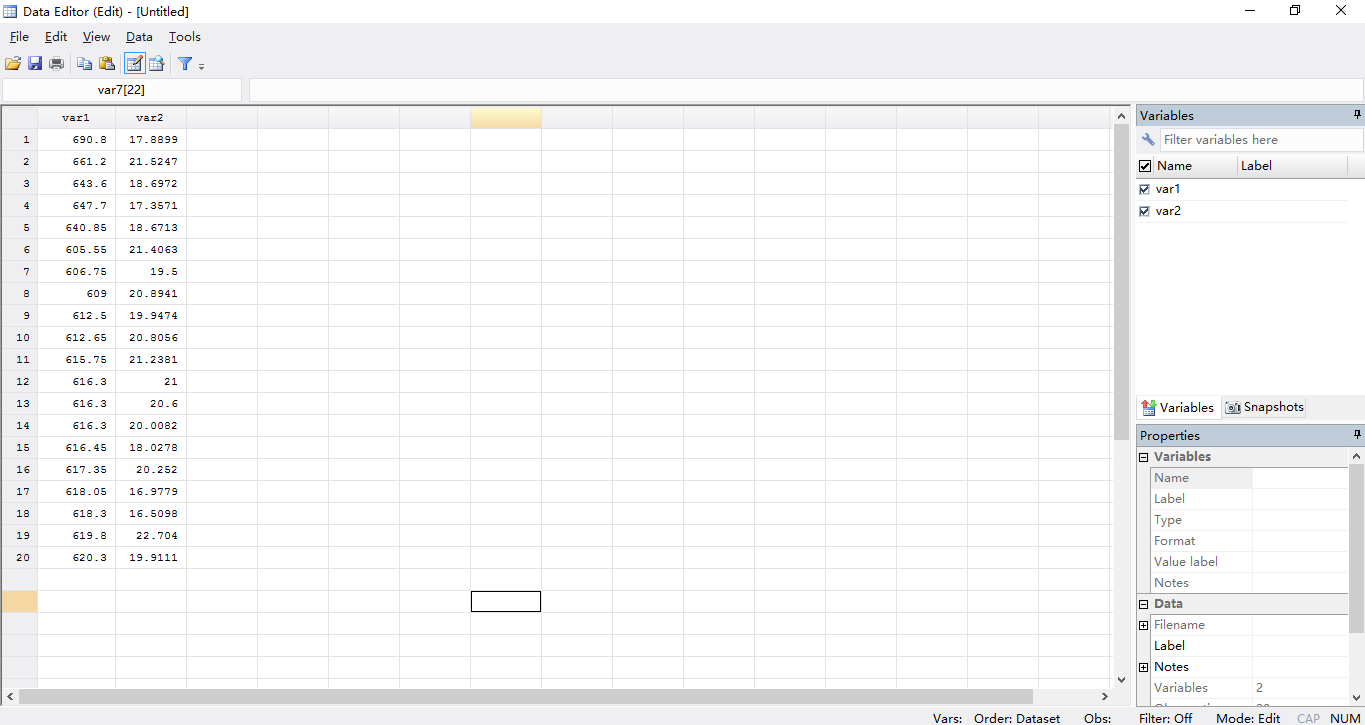
\includegraphics[width=1\textwidth]{data edit1.png}
		\caption{数据输入界面}\label{fig:digit}
	\end{figure}
	
	单击第一列的灰色方框,可以看到右侧下窗口“properties”变成
	\begin{figure}[htbp]
		\centering
		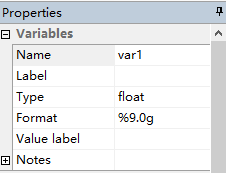
\includegraphics[width=0.5\textwidth]{properties.png}
		\caption{数据输入界面}\label{fig:digit}
	\end{figure}
	
	单击其中的“name”,修改“var1”为“testscr”。同理,也可以把“var2”修改为“str”。得到下图的数据输入结果。
	\begin{figure}[htbp]
		\centering
		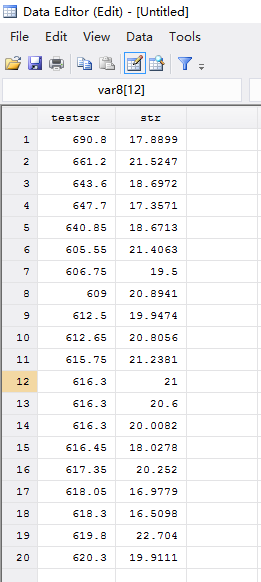
\includegraphics[width=0.5\textwidth]{data edit2.png}
		\caption{数据输入界面}\label{fig:digit}
	\end{figure}
	
	与此同时,我们还可以在stata主面板上看到如下结果
	\begin{figure}[htbp]
		\centering
		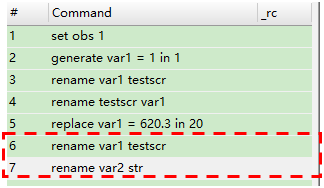
\includegraphics[width=0.5\textwidth]{command.png}
		\caption{数据输入界面}\label{fig:digit}
	\end{figure}
	
	\begin{figure}[htbp]
		\centering
		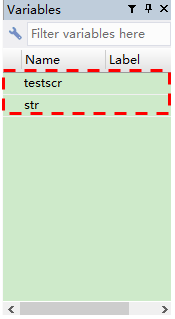
\includegraphics[width=0.5\textwidth]{variables.png}
		\caption{数据输入界面}\label{fig:digit}
	\end{figure}
	
	\begin{figure}[htbp]
		\centering
		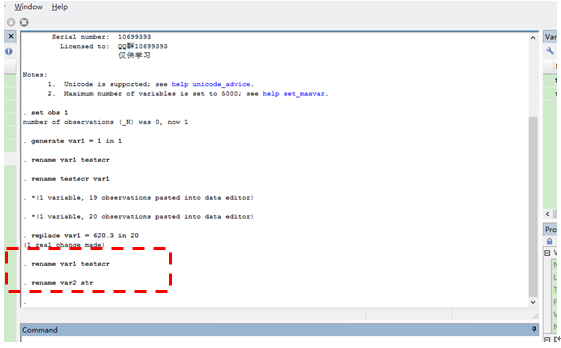
\includegraphics[width=0.7\textwidth]{windows1.png}
		\caption{数据输入界面}\label{fig:digit}
	\end{figure}
	
	打开data editor(edit)的另一种方式是点击菜单栏中的表格按钮“data editor(edit)”。
	
	这样输入数据很麻烦,也会出很多错误。下面还会介绍另一种输入数据的方式。
	
	通常,我们会查看一下现存的一些变量,可以输入下列命令
	\begin{table}[htbp]
		\centering
		\begin{tabular}{|l|}
			\hline
			list\quad varname1\quad varname2\quad \dots \\
			\hline
		\end{tabular}
	\end{table}
	
	我们上面的变量名,所要输入的命令是
	
	\textbf{list\quad testscr\quad str}
	
	这个命令将会把所有变量的观测值都列示在结果窗口中。缺失数据会用“.”表示。但是一旦样本量大了,这种列示所有观测数据的方法就不适用了。要想终值列示进程,可以点击菜单栏中的“break”按钮。以后再介绍另一些检查错误的方式。你会看到如下界面
	\begin{figure}[htbp]
		\centering
		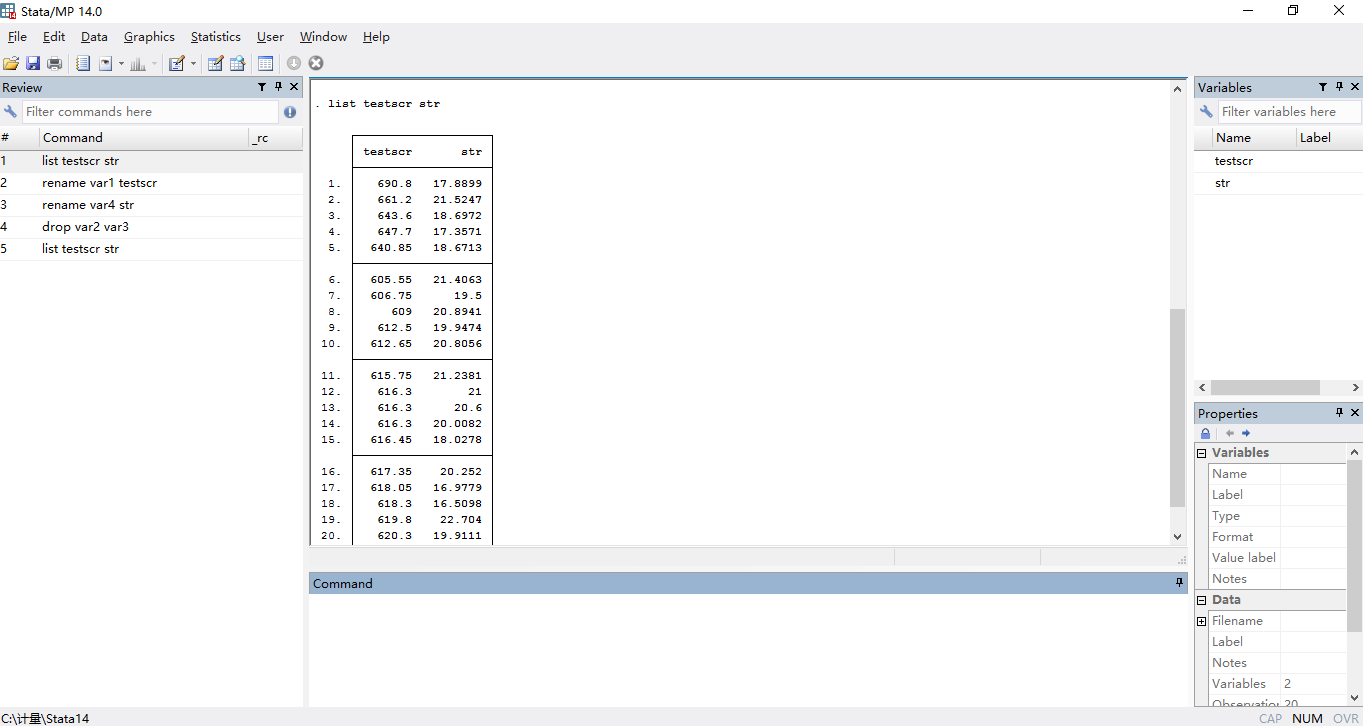
\includegraphics[width=0.7\textwidth]{list.png}
		\caption{观测值列表}\label{fig:digit}
	\end{figure}
	
	如本讲中,我们需要知道样本数据的统计特征。我们可以输入如下命令
	
	\textbf{sum\quad testscr\quad str,detail}
	
	我们可以得到下图
	\begin{figure}[htbp]
		\centering
		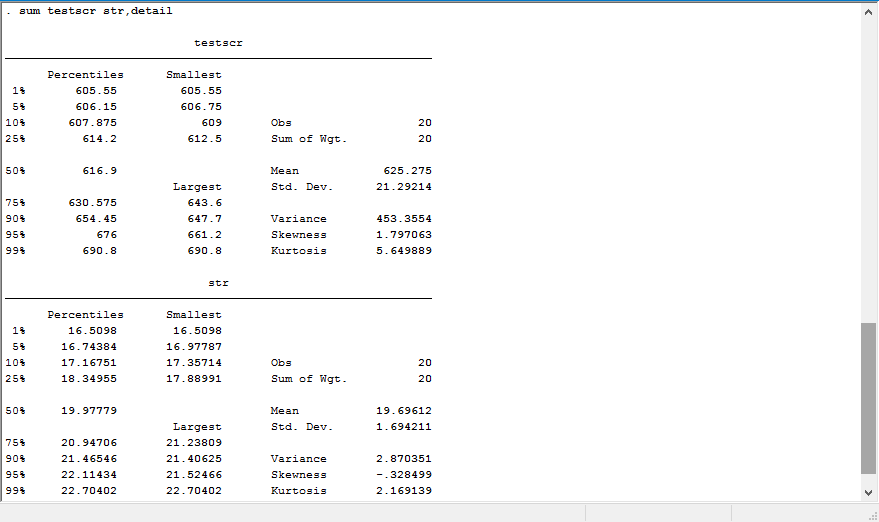
\includegraphics[width=0.7\textwidth]{sum.png}
		\caption{统计量}\label{fig:digit}
	\end{figure}
	
	散点图的命令为
	
	\textbf{scatter\quad testscr\quad str}
	
	得到的图形如下
	\begin{figure}[htbp]
		\centering
		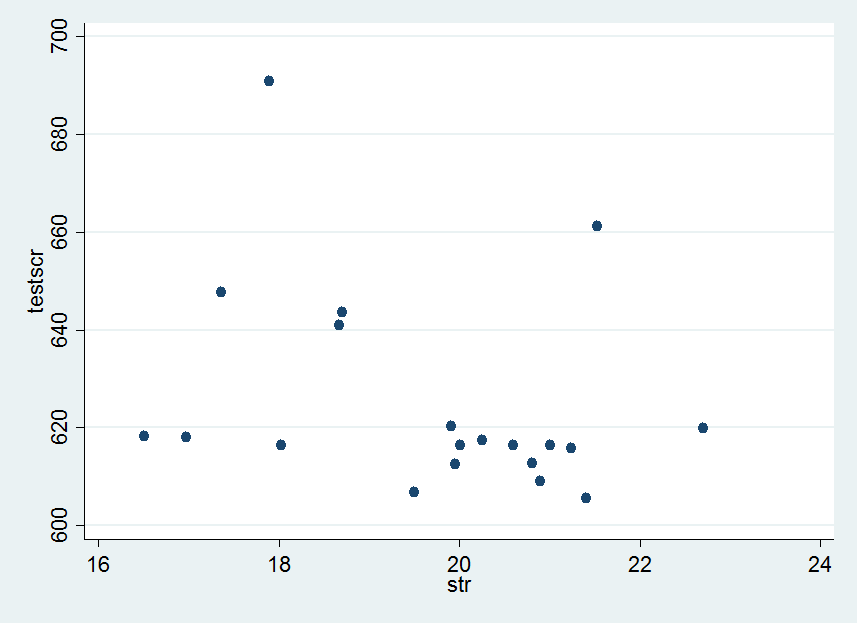
\includegraphics[width=0.7\textwidth]{Graph.png}
		\caption{散点图}\label{fig:digit}
	\end{figure}
	
	我们还想看看散点图的拟合线。命令如下
	
	\textbf{twoway\quad scatter\quad testscr\quad str\quad || lfit\quad testscr\quad str}
	
	得到的图如下:
	\begin{figure}[htbp]
		\centering
		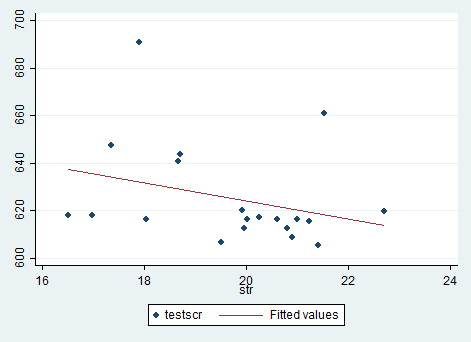
\includegraphics[width=0.7\textwidth]{line.png}
		\caption{拟合线}\label{fig:digit}
	\end{figure}
	
	而简单的回归的命令为
	
	\textbf{reg\quad testscr\quad str}
	
	得到的结果如下
	\begin{figure}[htbp]
		\centering
		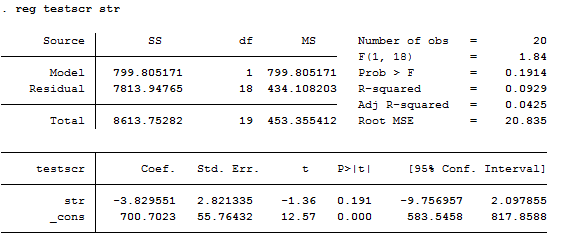
\includegraphics[width=0.7\textwidth]{reg.png}
		\caption{简单回归结果}\label{fig:digit}
	\end{figure}
	
	而稳健标准误的回归命令为
	
	\textbf{reg\quad testscr\quad str,r}
	
	得到的结果如下
	\begin{figure}[htbp]
		\centering
		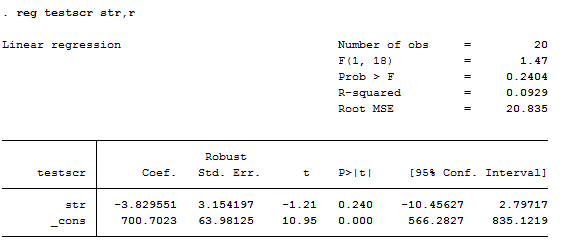
\includegraphics[width=0.7\textwidth]{regr.png}
		\caption{稳健标准误回归结果}\label{fig:digit}
	\end{figure}
	

	\chapter{多元线性回归}

	第三讲的回归结果显示:学生老师比越小,平均分数越高。但是,肯定有人怀疑这一结论,因为小班的学生可能还有其他的因素使得其平均分数更高。
	
	在第三讲中,这些被遗漏的因素全部“丢进”了误差项$u_i$中。但是这会使得OLS估计量产生偏误,我们在下面的内容中将详细阐述。那么,怎么解决“遗漏变量偏误”呢?\textbf{多元回归}就是消除遗漏变量偏误的一种方法。
	
	多元回归的idea很直观:如果那些遗漏变量的数据可用,那么,我们就能将这些变量纳入回归方程中作为回归因子,并且在保持其它变量不变的情况下,估计出一个回归因子的效应。
	
	\section{遗漏变量偏误}
	第三讲用小班教学作为例子。在这个例子中,班级规模(学生- 老师比)越小,平均成绩越高。但是,仅仅考虑学生-老师比这一个因素不够,还忽略了许多重要的潜在决定因素对测试成绩的影响。这些潜在影响因素包括:学校特征(教师质量、硬件设备等等)、学生特征(家庭背景、语言差异等等)。下面,我们以语言差异为例。
	
	大家都知道,中国方言甚多,甚至同一个城市里不同区域的方言也不相同。在湖北省高考语文试题中,经常考字的读音。湖北人普通话不标准,因为前鼻音“l” 和后鼻音“n”不分,平舌“si”和翘舌“shi"不分。还有很多的地方的人“飞”和“灰”不分。因此,估计很多学生都怕读音题,尤其是是南方人。
	
	那么,如果一个班里南方人比例多,而另一个班级里北方人比例高,如果考读音题,估计南方人多的班级平均分会低于北方人多的班级。如果我们忽略这种语言差异,仅仅用学生-老师比来回归,预期班级规模对测试成绩的效应会有偏。因为南方学生在读音题上的得分可能低于北方学生。如果大班中有许多南方人,那么,学生-老师比的OLS回归系数可能会高估对测试分数的效应。
	
	\subsection{遗漏变量偏误的定义}
	如果一个回归元与模型中遗漏的变量有关,且这个遗漏变量还是因变量的决定因素,那么,OLS 估计量会产生\textbf{遗漏变量偏误}。
	
	遗漏变量偏误产生必须同时满足两个条件:
	
	1、X与遗漏变量相关;
	
	2、遗漏变量是因变量Y的一个决定因素。
	
	\textbf{遗漏变量偏误与第一个LS假设。}回顾一下第三讲中有关OLS的三个假设,其中,第一个是$E(u_i|X_i)=0$。遗漏变量偏误就意味着这个假设不成立。
	
	在一元回归中,$u_i$包含除了$X_i$以外所有决定Y的因素。如果这些遗漏的因素中有一个与$X_i$,那么,误差项$u_i$就与$X_i$相关。因此,$E(u_i|X_i)\neq0$。这个假设不成立,后果很严重:OLS估计量有偏。即使在大样本下,偏误也不会消除,而且OLS估计量不是一致估计量。
	
	因为,遗漏变量与$X_i$相关,我们定义$corr(X_i,u_i)=\rho_{Xu}$。 假设LS 的第二和第三个假设仍然成立。那么,OLS估计量就有下列极限:
	\begin{equation}
		\hat{\beta}_1\xrightarrow{p}\beta{_1}+\rho_{Xu}\frac{\sigma{_u}}{\sigma{_X}}
	\end{equation}
	
	也就是说,随着样本规模的增大,$\hat{\beta}_1$以越来越高的概率趋近于$\ beta{_1}+\rho_{Xu}\frac{\sigma{_u}}{\sigma{_X}}$。
	
	\textbf{note}:
	
	1、无论样本规模大小,遗漏变量偏误问题都要引起注意。从公式(1)中可以看出,$\hat{\beta}_1$并不收敛到真值$\beta_1$。且偏误的大小为$\rho_{Xu}\frac{\sigma{_u}}{\sigma{_X}}$。
	
	2、偏误的大小取决于误差项与X 的相关系数$\rho_{Xu}$。$|\rho_{Xu}|$越大,偏误越大。
	
	3、偏误的方向(也就是,系数高估还是低估)取决于误差项与X是正相关还是负相关。如果$\rho_{Xu}<0$,OLS估计量就是低估,反之亦然。
	
	\textbf{例子:听莫扎特可以提高智力?!}
	
	在孩子教育问题方面,流传着这样的一个故事:让孩子每天听听莫扎特的音乐,可以提高孩子的智力。其实,这是Rauscher et al.(1993)在Nature上发表的研究成果。他们建议,听10-15 分钟的莫扎特会暂时性提高IQ8-9个点。
	
	真的存在“莫扎特效应”吗?如果存在,提高8-9点IQ是高还是低了?现在我们学了一点计量了,我们用计量经济学的语言,这个效应估计可能存在遗漏变量偏误。
	
	\section{多元回归模型}
	既然遗漏变量偏误是由于某些决定Y,而又与X相关的变量没有包含在回归方程中,那么,只要这些变量数据可用,我们只要把它们纳入回归方程中就可以消除遗漏变量偏误。这就是\textbf{多元回归模型}。多元回归模型可以在保持$X_2$不变的情况下,估计出$X_1$对Y的效应。
	
	\textbf{总体回归线}
	
	假设只有两个自变量$X_{1i}$和$X_{2i}$。在线性多元回归模型中,自变量和因变量之间的关系由下式给出
	\begin{equation}
		E(Y_i|X_{1i}=x_1,X_{2i}=x_2)=\beta_0+\beta_1x_1+\beta_2x_2
	\end{equation}
	
	公式(2)称为\textbf{总体回归线,或者总体回归函数}。多元回归模型中一个或多个自变量有时候也称为\textbf{控制变量}。公式(2)中的系数$\beta_1$含义与一元回归中有些不同。在多元回归中,这个系数是保持X2为常数或者控制X2 时,X1的单位变化引起Y的变化。这个系数也称为\textbf{局部效应}。
	
	\textbf{总体回归方程}
	
	正如一元回归,多元回归线也不能精确表示自变量与Y之间的关系,因为还有许多影响Y的因素并没有包含在多元回归线中。因此,公式(2)也需要包含误差项来代表其它因素。即
	\begin{equation}
		Y_i=\beta_0+\beta_1X_1+\beta_2X_2+u_i,~~i=1,\cdots,n
	\end{equation}
	
	我们可以把$\beta_0$理解成是值为1的自变量的系数。因为该自变量的值恒为1,因此称为常自变量。类似,$\beta_0$也被称为\textbf{常数项}。
	
	在实践中,多元回归模型通常包含两个以上的自变量,形式如下
	\begin{equation}
		Y_i=\beta_0+\beta_1X_1+\beta_2X_2+\cdots+\beta_kX_k+u_i,~~i=1,\cdots,n
	\end{equation}
	
	\subsection{多元回归中的OLS估计量}
	回忆一下,一元回归的OLS估计量:选择系数来最小化预测误差平方和,即选择$\hat{\beta}_0,\hat{\beta}_1$ 来最小化$\sum_{i=1}^{n}{(Y_i-\hat{\beta}_0-\hat{\beta}_1X_i)^2}$。$\hat{\beta}_0,\hat{\beta}_1$ 就是OLS估计量。
	
	这一思想也可以沿用至多元回归的系数估计。即
	\begin{equation}
		\sum_{i=1}^{n}{(Y_i-\hat{\beta}_0-\hat{\beta}_1X_i-\cdots-\hat{\beta}_kX_k)^2}
	\end{equation}
	
	其中,$\hat{\beta}_0,\hat{\beta}_1,\cdots,\hat{\beta}_k$ 是OLS估计量。而OLS残差用$\hat{u}_i=Y_i-\hat{Y}_i$表示。
	
	上面的OLS估计量公式有点麻烦。但是,幸运地是这些计算公式都已经编写进了统计软件中,例如Stata,我们把数据输入后,软件就可以直接给出结果。
	
	\textbf{应用}
	
	第三讲中,学生-老师比对测试成绩的效应,用的美帝加利福利亚州420个观测样本估计的回归模型为
	\begin{equation}
		\hat{Y}=698.9-2.28\times{X}
	\end{equation}
	
	但是,通过上面内容的讲解,我们担心这个回归模型对小班教学效应的估计不准确。因为它存在遗漏变量偏误问题。因为美帝是一个移民国家,学校里有许多学生母语是非英语,因此,其在测试分数上表现稍微差一些。我们正好也有加利福利亚州学生母语为非英语人数的数据。那么,我们就可以在上述一元回归模型中引入非母语学生变量,从而消除遗漏变量偏误问题。得到的多元回归方程为
	\begin{equation}
		\hat{Y}=686.0-1.10\times{X_1}-0.65\times{X_2}
	\end{equation}
	
	其中,$X_1$表示学生-老师比(str),$X_2$表示非英语母语学生(elpct)。
	
	stata结果为
	\begin{figure}[htbp]
		\centering
		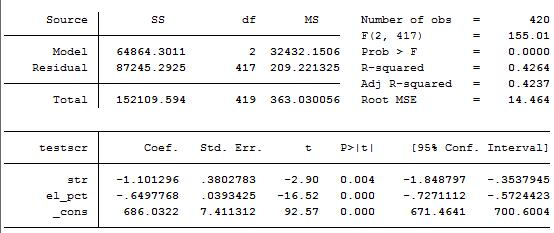
\includegraphics[width=0.7\textwidth]{mreg.jpg}
		\caption{多元回归结果}\label{fig:digit}
	\end{figure}
	
	将一元回归方程(6)和多元回归方程(7)中,学生-老师比对测试分数的效应的OLS估计结果进行对比。多元回归中,$\beta_1$的OLS估计量为-1.10,这几乎是一元回归估计量的一半。也就是说,多元回归中班级规模对测试分数的效应是一元回归中估计地效应的一半。这是因为在多元回归中,-1.10 表示保持$X_2$不变时,班级规模的效应,而-2.28则表示班级规模与非英语母语学生都在变化时的效应。
	
	这种对比也可以看出,一元回归存在遗漏变量偏误。估计出的班级规模效应偏大。
	
	\subsection{拟合度}
	与一元回归类似,多元回归也有三个常用的统计量来检验回归方程对数据的拟合程度,它们分别是:$SER$、$R^2$和调整$R^2$ ($\overline{R}^2$)。
	
	\textbf{SER}
	
	SER估计误差项$u_i$的标准差。在多元回归中,SER为
	\begin{equation}
		SER=s_{\hat{u}}=\sqrt{s_{\hat{u}}^2}~where~s_{\hat{u}}^2=\frac{1}{n-k-1}\sum_{i=1}^{n}{\hat{u}_i^2}=\frac{SSR}{n-k-1}
	\end{equation}
	
	上式与第三讲中的SER公式的差异在分母是$n-k-1$,而不是$n-2$。第三讲中,除数$n-2$是为了调整由估计两个系数而引起的向下偏误。而此处$n-k-1$则是为了调整估计$k+1$ 个系数(k个斜率和一个截距)引起的向下偏误。$n-k-1$ 成为\textbf{自由度}。当n很大时,自由度调整可以忽略。
	
	\textbf{$R^2$}
	
	回忆一下,第三讲中$R^2$定义为回归因子所能解释的$Y_i$的样本方差比例,或者1减回归因子不能解释的样本方差比例。即
	\begin{equation}
		R^2=\frac{ESS}{TSS}=1-\frac{SSR}{TSS}
	\end{equation}
	
	其中,回归平方和$ESS=\sum_{i=1}^n{(\hat{Y}_i-\overline{Y})^2}$,总平方和$TSS=\sum_{i=1}^n{(Y_i-\overline{Y})^2}$。
	
	多元回归中的$R^2$定义同上。但是,特别需要注意的是,\textbf{除非增加的回归量的系数为0,否则随着回归量的增加,$R^2$逐渐增大。}根据OLS,选择系数值来最小化残差平方和SSR。(1)如果增加的回归量的系数为0,那么,SSR 不会随着这个增加的回归量而变化。(2)如果增加的回归量系数不为0,那么,增加该回归量之后的SSR会变小,从公式(9)可知,$R^2$变大。
	
	那么,增加回归量,$R^2$变大,是否意味着增加回归量就提高了模型的拟合程度呢?答案是否定的。因此,就需要纠正多元回归中的$R^2$,为此,提出了调整的$R^2$,即$\overline{R}^2$
	\begin{equation}
		\overline{R}^2=1-\frac{n-1}{n-k-1}\frac{SSR}{TSS}=1-\frac{s_{\hat{u}}^2}{s_Y^2}
	\end{equation}
	
	公式(10)与(9)之间的差别就是残差平方和与总平方和之比前面成了一个因子($\frac{n-1}{n-k-1}$)。关于$\overline{R}^2$有三点需要注意:
	
	第一,$\frac{n-1}{n-k-1}$总是大于1,因此,$\overline{R}^2<R^2$;
	
	第二,增加一个回归量对$\overline{R}^2$有正负两个方面的影响,一方面,SSR下降,$\overline{R}^2$上升;另一方面,因子$\frac{n-1}{n-k-1}$变大,$\overline{R}^2$ 变小。因此,$\overline{R}^2$变大变小取决于这两个效应谁占主导地位;
	
	第三,$\overline{R}^2$可以为负数。当增加回归量,SSR下降的程度不足以抵补$\frac{n-1}{n-k-1}$的下降,那么$\overline{R}^2$就可能为负。
	
	\textbf{示例:}从上文的图1中可以看出,$R^2=0.4264$,而$\overline{R}^2=0.4237$,$SER=14.464$。将这些结果与第三讲中的一元回归结果进行对比,$R^2$从0.051上升到0.4264,也就是说只有学生-老师比这一个自变量时,自变量只能解释测试分数方差的5.1\%,而增加非英语母语学生这个自变量时,两个自变量可以解释测试分数方差的42.64\%。从这个意义上看,增加一个自变量确实提高了回归模型的拟合程度。因为样本量$n=420$,回归量$k=2$,因此,$R^2$ 与$\overline{R}^2$ 之间的差异就非常小。
	
	此外,SER也从一元回归的18.6上升到多元回归的14.5,这也说明拟合的更好。
	
	\textbf{提醒:}虽然$\overline{R}^2$与$R^2$很有用,但是太依赖于$\overline{R}^2$就会掉进陷阱。在实际应用中,“最大化$\overline{R}^2$” 几乎不能回答任何有意义的计量或统计问题。相反,是否要增加一个变量应该基于增加这个变量可以更好的估计出我们感兴趣的因果效应。
	
	\subsection{多元回归中的OLS假设}
	与一元回归类似,多元回归中OLS也有一些假设:
	\begin{equation}
		Y_i=\beta_0+\beta_1X_1+\beta_2X_2+\cdots+\beta_kX_k+u_i,~~i=1,\cdots,n
	\end{equation}
	
	其中,
	
	1、给定$X_{1i},X_{2i},\cdots,X_{ki}$的条件下,$u_i$的条件均值为0,即$E(u_i|X_{1i},X_{2i},\cdots,X_{ki})=0$;
	
	2、$(X_{1i},X_{2i},\cdots,X_{ki},Y_i)$独立同分布(i.i.d.);
	
	3、不可能出现较大奇异值:$X_{1i},X_{2i},\cdots,X_{ki},Y_i$有非零有限的四阶矩;
	
	4、不存在完全多重共线。
	
	\section{假设检验与置信区间}
	多元回归为消除遗漏变量偏误问题提供了一种方法。但多元回归中的OLS估计量也存在抽样不确定性。与一元回归不同,多元回归的假设可能包含两个或多个回归系数。检验这种“联合”假设的统计量,称为\textbf{F统计量}。
	
	\subsection{单系数假设检验与置信区间}
	回忆一下,一元回归系数的方差是由第三讲公式(20)给出的。在LS假设下,大数法则意味着样本均值会收敛到总体均值,因此,$\frac{\hat{\sigma}_{\hat{\beta}_1}^2}{\sigma_{\hat{\beta}_1}^2}\xrightarrow{p}1$。$\sigma_{\hat{\beta}_1}^2$ 的平方根就是$\hat{\beta}_1$的标准误,$SE(\hat{\beta}_1)$。
	
	这个计算标准误的方法也可以推广至多元回归。
	
	\subsubsection{单系数假设检验}
	一般来讲,我们想要检验多元回归第j个自变量的系数$\beta_j$等于某一确定值$\beta_{j,0}$。这个特定的值要么来源于经济理论,要么来源于实际应用中的决策值。如果备择假设是双边假设,那么,原假设与备择假设为
	\begin{equation}
		H_0:\beta_j=\beta_{j,0}~~vs.~~H_1:\beta_j\neq\beta_{j,0}
	\end{equation}
	
	例如,在小班教学的例子中,原假设就是$\beta_1=0$。我们的任务就是要用样本数据来检验原假设和备择假设。
	
	与一元回归的假设检验步骤类似,多元回归假设检验步骤如下:
	
	第一步,计算$\hat{\beta}_j$的标准误,$SE(\hat{\beta}_j)$;
	
	第二步,计算t统计量
	\begin{equation}
		t=\frac{\hat{\beta}_j-\beta_{j,0}}{SE(\hat{\beta}_j)}
	\end{equation}
	
	第三步,计算p值
	\begin{equation}
		p=2\Phi(-|t^{act}|)
	\end{equation}
	其中,$t^{act}$是计算出来的实际t统计量。如果p值小于0.05或者$|t^{act}|>1.96$,那么就在5\%的显著性水平下拒绝原假设。
	
	注:我们从上面的stata结果可以看出,标准误、t统计和p值都是由软件自动输出的。
	\begin{figure}[htbp]
		\centering
		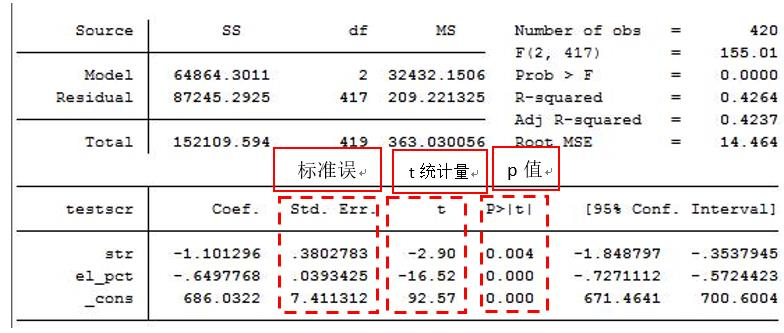
\includegraphics[width=0.7\textwidth]{SE.jpg}
		\caption{标准误、t统计量和p值}\label{fig:digit}
	\end{figure}
	
	\subsubsection{置信区间}
	多元回归的置信区间与一元回归相同。
	
	例如,系数$\beta_j$的95\%的双边置信区间以95\%的概率包含$\beta_j$的真实值。等价地,$\beta_j$的一系列值不能被5\%的双边假设检验所拒绝。当样本规模很大时,95\% 的置信区间为
	\begin{equation}
		95\%~conf. interval=[\hat{\beta}_j-1.96SE(\hat{\beta}_j),\hat{\beta}_j+1.96SE(\hat{\beta}_j)]
	\end{equation}
	注:如果是90\%的置信区间,就用1.64代替1.96;如果是99\%的置信区间,就用2.58取代1.96。
	
	\textbf{提醒:}无论是假设检验的方法和置信区间的方法都依赖于大样本正态近似于OLS估计量的分布。因此,要时刻记住这些量化抽样不确定性的方法仅仅在大样本下才起作用。
	
	\textbf{示例1:图2}
	
	由图2的多元回归结果可知,学生-老师比的系数为-1.10,SER为0.38,而原假设为$\beta_1=0$,因此,t值为$\frac{-1.10-0}{0.38}=-2.89$,这一结果与图2中显示的一致。对应的p值为0.4\%,因为p值小于5\%,所以在5\%的显著性水平下拒绝原假设(这个值甚至小于1\%的显著性水平)。
	
	由图2还可知道95\%的置信区间为$[-1.85,-0.35]$。
	
	\textbf{示例2:加入其它控制变量}
	
	假设还有其它因素影响测试成绩,例如生均教师支出(expn)。那么,将生教师均支出加入回归方程后的结果为
	\begin{figure}[htbp]
		\centering
		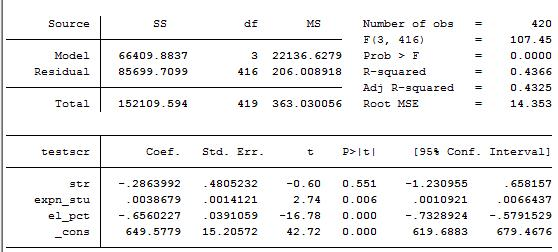
\includegraphics[width=0.7\textwidth]{expn.jpg}
		\caption{加入生均支出的回归结果}\label{fig:digit}
	\end{figure}
	
	从图3中,我们看到了十分有趣的结果:加入expn之后,str(学生-老师比)的效应更小了,仅为-0.286,而且t统计量仅为-0.6,对应的p值为0.551。也就是说,总体回归中这个系数为0的假设不能在10\%的显著性水平下被拒绝。\textbf{其经济含义就是,保持生均教师支出和非英语母语学生不变的情况下,没有证据显示,小班教学会提高测试成绩。}
	
	从这个结果还可以有另一种理解或推断:教育管理部门有效地批准了教育资金。假设一种相反的结果,加入生均教师支出后,str的系数很大,且为负。那么,教育管理部门只需要减少其它的教育支出(例如,课本、教学设备等等),而将其用于雇佣更多的教师。这样既可以保持教育支出不变,也而缩减班级规模,从而使得测试成绩提高。但是上面的回归结果却是str的系数很小,且统计不显著,这也就意味着将其他教育支出转移至教师支出这种资金配置不会对测试成绩的提高产生效应。从而推断出教育管理部门有效地配置了教育资金。
	
	\textbf{小贴士:}从图3中,str的标准误从图2中的0.38变为图3中的0.48,这说明str和expn可能存在多重共线性。而多重共线性会导致OLS估计不精确。
	
	\subsection{联合假设检验}
	如果原假设为学生-老师比和生均支出的系数同时为0,该如何检验呢?
	
	我们控制非英语母语学生变量,联合假设为
	\begin{equation}
		H_0:\beta_1=0,\beta_2=0~~vs.~~H_1:\beta_1\neq0,\beta_2\neq0
	\end{equation}
	
	\textbf{联合假设}就是对两个或多个回归系数施加限制。只要原假设中的任何一个系数等式不成立,那么,联合原假设就为假。
	
	那么,我们为什么不能一次检验一个系数呢?
	
	如果我们对上述联合假设检验感兴趣,并分别用$t_1$和$t_2$来检验第一个系数为0和第二个系数为0。那么,只要$t_1$和$t_2$中有一个大于1.96就应该拒绝原假设?
	
	由于这个问题中涉及两个随机变量$t_1$和$t_2$,因此,需要刻画它们的联合抽样分布。在大样本下,$\beta_1$和$\beta_2$有联合正态分布,因此,$t_1$ 和$t_2$有一个双变量正态分布。假设两个t统计量不相关且独立。那么,不能拒绝原假设当且仅当$|t_1|\geq1.96,|t_2|\geq1.96$。$Pr(|t_1|\geq1.96,|t_2|\geq1.96)=0.95^2=0.9025$。 因此,拒绝原假设的概率为9.57\%(1-0.9025)。
	
	如果这两个t统计量相关,那么,这种情形更加复杂。但是“一次检验一个”的方法不会得到一个合意的显著性水平。而另一种法就是基于F统计量的检验。
	
	\subsubsection{F统计量}
	F统计量用于检验回归分析中的联合假设。Stata软件可以直接输出F统计量。当联合原假设为两个系数为0时,F统计量的公式为
	\begin{equation}
		F=\frac{1}{2}(\frac{t_1^2+t_2^2-2\hat{\rho}_{t_1,t_2}t_1t_2}{1-\hat{\rho}_{t_1,t_2}^2})
	\end{equation}
	其中,$\hat{\rho}_{t_1,t_2}$是两个t统计量相关系数的估计值。
	
	下面来看看q个系数的联合假设检验。大样本下,F统计量有$F_q^\infty$分布。因此,F统计量的临界值就能通过$F_{q,\infty}$分布表查出来,得到一个合适的显著性水平。F 统计量计算的p值为
	\begin{equation}
		p=Pr[F_{q,\infty}>F^{act}]
	\end{equation}
	
	上式计算出来的p值与F分布临界值对比。在给大家上课的时候,虽然把这些步骤都告诉大家,但是stata等软件直接帮我们略去了这些细节,直接给出结果。
	
	F统计量检验所有系数为0的联合假设。即原假设和备择假设为
	\begin{equation}
		H_0:\beta_1=0,\beta_2=0,\cdots,\beta_k=0~~vs.~~H_1:\beta_j\neq0,j=1,2,\cdots,k
	\end{equation}
	其中,备择假设说明至少有一个j不等于0。
	
	在原假设下,没有回归量能解释Y的方差。当$q=1$时,F统计量检验单一系数的限制。联合假设就退化成一元回归系数的假设,F统计量就是t统计量的平方。
	
	\textbf{示例}
	
	检验学生-老师比和生均支出的系数为0。计算F统计量为5.43。如下图所示
	\begin{figure}[htbp]
		\centering
		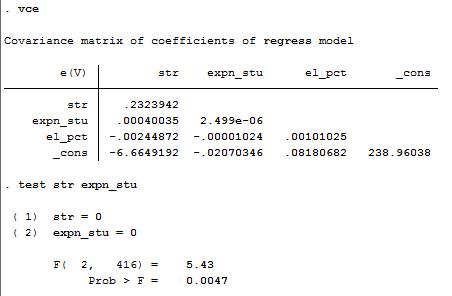
\includegraphics[width=0.7\textwidth]{F2.jpg}
		\caption{F统计量}\label{fig:digit}
	\end{figure}
	
	在原假设下,大样本性质使得F统计量有$F_{2,\infty}$分布。查F分布临界值表,$F_{2,\infty}$分,5\%的临界值为3.00,1\%的临界值为4.61。而计算得到的F统计量为5.43,大于1\%显著性水平下的临界值,因此,在1\%的显著性水平下拒绝原假设。
	
	\subsection{多元回归模型设定}
	多元回归中有两个或多个自变量,那么,如何决定哪些变量要放进多元回归中呢?目前,还没有“万能灵药”来应对所有情形。但是也不用失望,因为有许多指导性建议可用。选择一个变量作为自变量,应该从可能的遗漏变量偏误着手。这有赖于你们对经验问题的专业知识,由此获得一个无偏的因果效应。而不是仅仅完全依赖于统计拟合程度,例如$R^2$和$\overline{R}^2$。
	
	回忆一下,本讲第一节提到的遗漏变量偏误,必须满足两个条件:(1)至少有一个回归量与遗漏变量相关;(2)遗漏变量必须是因变量Y的决定因素。
	
	这也就意味着给定$X_1i,X_2i,\cdots,X_ki$,$u_i$的条件期望为非零,这就会打破LS第一个假设。因此,即使在大样本下,遗漏变量偏误还是会存在。即是说,遗漏变量偏误使得OLS估计量非一致。
	
	上面的例子隐含着核心解释变量(我们希望估计的因果效应)和控制变量。
	
	\textbf{控制变量}并不是我们感兴趣的目标;它们是包含在多元回归中,保持为不变的因素;如果忽略它们就会导致感兴趣变量(核心解释变量)的因果效应遭遇遗漏变量偏误。
	
	在LS第一假设上,我们来区别对待核心解释变量和控制变量。核心解释变量的OLS估计量是无偏的,但是控制变量的OLS估计量一般来讲是有偏的,因此并没有因果含义。
	
	\textbf{示例}
	
	考虑由于遗漏外部学习机会而引起的潜在遗漏变量偏误。外部学习机会非常抽象和广泛,因此,很难测量。但是这些机会与学生的经济背景有关,而经济背景可以测量。因此,经济背景就可以加入多元回归中,进而控制收入相关的遗漏因素。例如,我们在str和pctel之外,再加入受到免费午餐的学生比例(lchpct)。那么回归结果为
	
	\textbf{理论和实践中的模型设定}
	从理论来讲,如果遗漏变量数据可用,解决遗漏变量偏误,只需要在回归模型中加入遗漏变量即可。然而,在实践中,决定是否加入一个变量非常困难,并要三思而行。
	
	从实践来看,应对遗漏变量偏误的方法:
	
	基础解释变量集应用依靠专业判断、经济理论以及对数据的了解,并进行综合决策。包含基础解释变量的集合有时也称为\textbf{基准模型}。
	
	第一步,基准模型应该包含主要的核心解释变量和控制变量,这些变量是根据专业判断和经济理论得到的。
	
	第二步,有经济理论得到的变量经常没有可用的数据,那么,就需要提出许多备择模型设定,即一些备择的回归因子。
	
	\textbf{如果在备择模型中,核心解释变量的数值与基准模型相似,这就说明基准模型的估计结果可信。另一方面,如果核心解释变量的估计结果在备择模型中变化较大,那么,这说明基准模型存在遗漏变量偏误。}我们将在第五讲中详细阐述遗漏变量偏误及其解决办法。
	
	实践中,$R^2$和$\overline{R}^2$能告诉我们什么?不能告诉我们什么呢?
	
	$R^2$和$\overline{R}^2$\textbf{能告诉我们}回归因子解释因变量的方差的程度。如果$R^2$或$\overline{R}^2$接近于1,说明回归因子能作出对因变量的较好预测,才能够这个意义上来讲,OLS残差方法较小。如果$R^2$或$\overline{R}^2$接近于0,情况相反。
	
	$R^2$和$\overline{R}^2$\textbf{不能告诉我们}
	
	(1)一个解释变量是否统计显著;
	
	(2)回归因子是驱动因变量变动的真实原因;
	
	(3)存在遗漏变量偏误;
	
	(4)我们已经选择了最适合的解释变量集合。
	
	\section{多元回归Stata操作示例}
	这一节,我将利用小班教学的数据作为例子,来展示多元回归的stata操作及其结果分析与讨论。主要目的是为了说明利用多元回归如何消除遗漏变量偏误。
	
	\textbf{第一步,基准模型和备择模型的设定}
	
	从前面的讲稿内容可以看出,我们关心的班级规模(学生-老师比)对测试成绩的效应,且控制了学生的特征(例如,经济背景、非英语母语等)。除此之外,还有许多影响测试分数的潜在因素,且它们与学生-老师比相关。如果遗漏这些因素就会导致遗漏变量偏误。如果控制变量使得条件均值独立性假设成立,那么,学生-老师比的系数就是保持控制变量不变时班级规模对测试分数的效应。
	
	我们考虑三个学生特征:非英语母语学生比例(elpct)、接受免费午餐的学生比例(mealpct)、有资格接受家庭收入援助的学生比例(calwpct)。后面两个变量都可以刻画学生的经济背景。经济理论和转专业判断并不能告诉我们这两个变量中哪一个作为控制变量代表学生经济特征更合适。因此,我们把免费午餐学生比例作为基准回归模型,而把接受家庭收入援助的学生比例作为备择回归模型。
	
	下面,我们分别作出测试分数(testscr)与非英语母语学生比例(elpct)、接受免费午餐的学生比例(mealpct)、有资格接受家庭收入援助的学生比例(calwpct)的散点图。
	
	我们在stata命令栏中分别输入
	
	\textbf{ scatter~testscr~elpct}
	
	\textbf{ scatter~testscr~mealpct}
	
	\textbf{ scatter~testscr~calwpct}
	
	可以得到下列三幅三点图
	\begin{figure}[htbp]
		\centering
		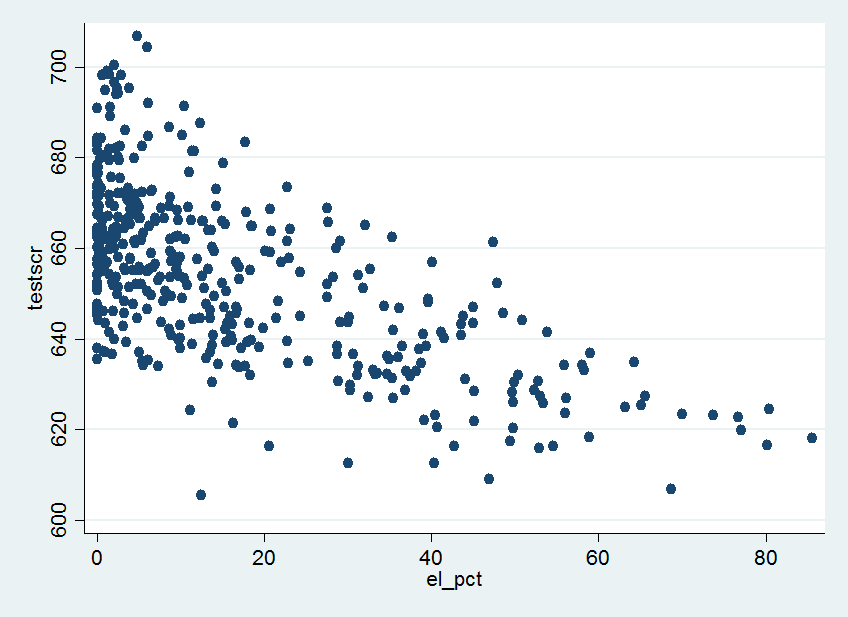
\includegraphics[width=0.7\textwidth]{elr.png}
		\caption{测试分数与非英语母语学生比例}\label{fig:digit}
	\end{figure}
	
	\begin{figure}[htbp]
		\centering
		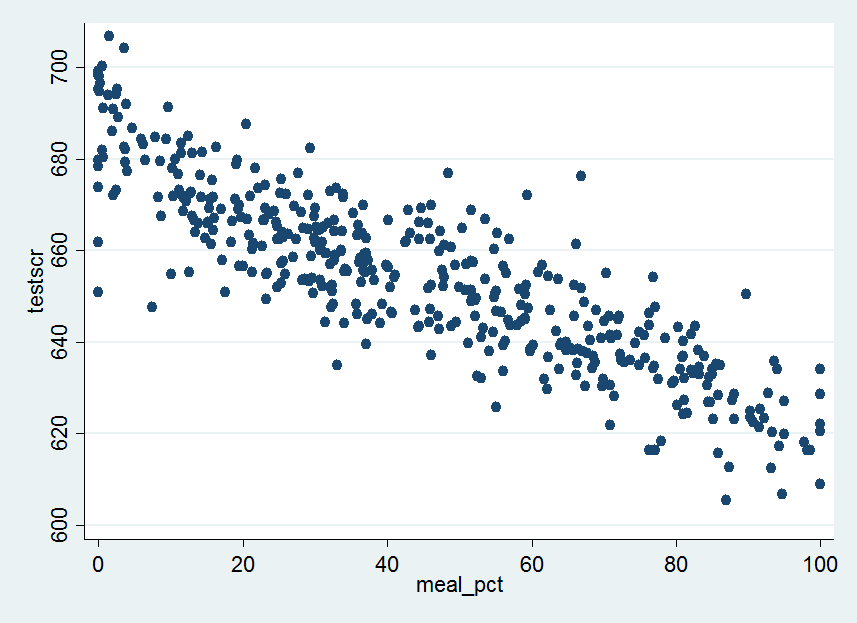
\includegraphics[width=0.7\textwidth]{lunch.png}
		\caption{测试分数与接受免费午餐的学生比例}\label{fig:digit}
	\end{figure}
	
	\begin{figure}[htbp]
		\centering
		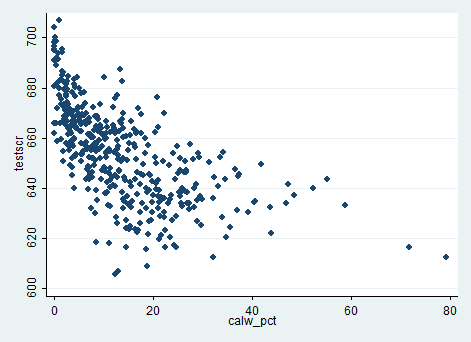
\includegraphics[width=0.7\textwidth]{income.png}
		\caption{测试分数与接受收入援助的学生比例}\label{fig:digit}
	\end{figure}
	
	还可以得到这些变量之间的相关系数。在stata命令栏输入
	
	\textbf{ cor~testscr~str~elpct~mealpct~calwpct}
	
	得到下列结果
	\begin{figure}[htbp]
		\centering
		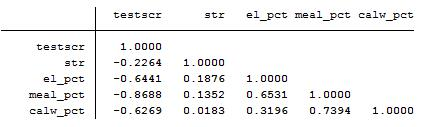
\includegraphics[width=0.7\textwidth]{corr.jpg}
		\caption{相关系数}\label{fig:digit}
	\end{figure}
	
	由上述结果可知,接受免费午餐的学生比例(mealpct)、有资格接受家庭收入援助的学生比例(calwpct)之间的相关系数为0.739。而测试分数与三个控制变量之间的均负相关,相关系数分别为-0.644、-0.869和-0.627。
	
	\textbf{小贴士}
	
	我们使用的三个控制变量都是学生比例,单位是百分号,那么,这些变量的范围肯定在0到100。同时,我们也可以用分数来表示这些变量,而不是百分数。那么,我们如何选择变量数值的量级或单位呢?
	
	这个问题的答案是选择一个变量的合适量级使得回归结果更容易读取和理解。例如,测试分数对学生-老师比和非英语母语学生比例的回归结果显示,非英语母语学生比例的回归系数为-0.650。如果非英语学生比例的量级换成$elpct/100$。回归模型的$R^2$和SER都不会变化,但是它的系数变成了-65.0。那么,在elpct的设定中,str保持不变,elpct的系数表示分数变化的百分点(分),而在$elpct/100$的设定中,str保持不变,$elpct/100$的系数表示100百分点的变化。尽管这两种模型设定在数学形式上是等价的,但是其OLS系数的含义还是前一种设定比较自然。
	
	\textbf{第二步,回归结果的呈现}
	
	基准回归模型和备择回归模型设定好了,stata会直接给出回归结果。那么,现在的问题来了,在这么多回归结果中,如何最好的呈现出回归结果呢?回忆一下,前面的内容已经以回归方程的形式呈现出了回归结果。但是这种形式在论文中很少见,论文中多数是以表格的形式呈现出回归结果。
	
	\begin{center}
		\begin{table}[!h]
			\caption{多元回归结果}\label{tab:digit}
			\begin{center}
				\begin{tabular}{lccccc}
					\hline
					自变量&(1)&(2)&(3)&(4)&(5)\\
					\cline{1-6}
					学生-老师比$X_1$&-2.280***&-1.101**&-0.998***&-1.308***&-1.014***\\
					&(0.519)&(0.433)&(0.270)&(0.339)&(0.269)\\
					
					非英语母语学生比例$X_2$&&-0.650***&-0.122***&-0.488***&-0.130***\\
					&&(0.031)&(0.033)&(0.030)&(0.036)\\
					
					免费午餐学生比例$X_3$&&&-0.547***&&-0.529***\\
					&&&(0.024)&&(0.038)\\
					
					收入援助学生比例$X_4$&&&&-0.790***&-0.048\\
					&&&&(0.068)&(0.059)\\
					
					常数项&698.933***&686.032***&700.15***&697.999***&700.392***\\
					&(10.364)&(8.728)&(5.568)&(6.920)&(5.537)\\
					\cline{1-6}
					SER&18.581&14.464&9.080&11.654&9.084\\
					
					$\hat{R}^2$&0.049&0.424&0.773&0.626&0.773\\
					
					F&19.26***&223.82***&453.48***&170.37***&361.68***\\
					
					obs&420&420&420&420&420\\
					\hline
				\end{tabular}
			\end{center}
		\end{table}
	\end{center}
	注:括号中为异方差稳健标准误;***、**、*分布表示1\%、5\%、10\%的显著性水平。
	
	表1呈现了五个回归模型的结果。第一列是自变量和统计量。从第二列至第六列,每一列代表一个多元回归模型。尽管表中没有呈现出t统计量,但是在实践中,括号里有时候是t统计量。因为在原假设下,回归系数、t统计量、SER和p 值可以相互计算得到。例如,(1)列中,$t=\frac{-2.28-0}{0.519}=-4.39$,而$4.39>2.58$,因此,该系数在1\%的显著性水平下显著。
	
	(2)-(5)列包含控制变量。(2)列结果在前文已经讲过。(3)列是基准模型结果,一个核心解释变量——学生-老师比,两个控制变量——非英语母语学生比例和免费午餐学生比例。(4)和(5)列则是备择模型结果,主要是对比学生经济特征变化的效应。(4)列是免费午餐学生比例作为控制变量,(5)列是在(4)基础上再加入收入援助项目学生比例作为控制变量。
	
	\textbf{第三步,经验结果分析}
	
	1、控制了学生特征之后,学生-老师比对测试分数的效应几乎减半。而且这个效应对模型中的控制变量并不敏感(或者十分稳健)。在所有的情形下,学生- 老师比的系数均在5\%的水平下显著。在四个带有控制变量的模型中,即从(2)到(5),保持学生特征不变时,每个老师减少一个学生的话,平均测试分数会上升1 分左右。
	
	2、学生特征的变量是测试分数的有效预测量。从(1)列看,$\hat{R}^2=0.049$说明,学生-老师比仅仅只能解释一小部分测试分数的变化。然而,当学生特征的变量加入回归模型后,$\hat{R}^2$大幅度上升。学生特征变量的系数符号与散点图中呈现的模式一致:非英语母语学生比例越高、家境贫寒学生比例越高的班级,平均测试分数越低。
	
	3、单个的控制变量并不总是显著:在(5)中,收入援助的学生比例对测试分数没有效应的原假设在5\%的显著性水平下不能被拒绝。由于把这个控制变量增加进基准模型(3)中,对核心解释变量(学生-老师比)的系数及其标准误都没有太大影响,且这个控制变量的系数不显著,因此,收入援助的学生比例对于我们的分析目的来说是多余的控制变量。
	
	\textbf{注:上述回归结果的stata命令为}
	\begin{figure}[htbp]
		\centering
		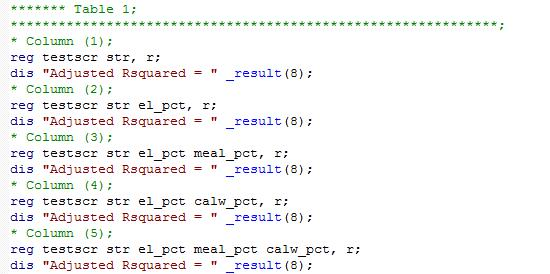
\includegraphics[width=1\textwidth]{cmd.jpg}
	\end{figure}


\chapter{识别的评价框架}

回归分析已经成为计量经济学领域最重要的经验研究方法。那么,自然出现的问题就是:我们如何评价基于回归分析的经验分析呢?或者如何判断采用回归分析方法的经验研究是否可信呢?

从第三讲和第四讲可以看出,一元回归会遗漏重要的回归量,从而导致我们关心的效应产生遗漏变量偏误,引入数据可用的遗漏变量,采用多元回归可以消除遗漏变量偏误。那么,如何评价我们所做的回归分析呢?

在本讲中,我会向大家介绍评价一个有用的经验研究的标准和步骤。如果发现回归分析的问题,应如何改进。

\section{内部有效性和外部有效性框架}
评价一个回归分析的有效性,要基于内部有效性和外部有效性的概念。如果一个研究关于因果效应的统计推断对于所研究的总体和环境是有效的,那么,这个研究就具有\textbf{内部有效性};如果这个研究德尔结论能推广至其他总体和环境,那么,它也具有\textbf{外部有效性}。

其中,\textbf{研究的总体}是研究所刻画的样本来源总体;\textbf{感兴趣的总体}是从研究中得到的因果推断推广应用的总体。例如,高中各种实验班对211、985高校升学率的效应,是否可以推广至高校各类实验班的设立呢。

而“环境”则是指制度、法律、社会、文化和经济环境等。例如,前面回归所得的美帝小班教学的效应,是否对中国有用呢?因为美帝和中国差异还是非常大的。

\subsection{内部有效性}
内部有效性由两部分构成:

1、因果效应估计量是无偏和一致的。

2、假设检验有合意的显著性水平,并且置信区间有合意的置信水平。

在回归分析中,因果效应是利用估计的回归函数来估算的,假设检验是利用估计的回归系数和标准误来执行的。因此,内部有效性要求OLS估计量是无偏和一致的,标准误的计算要使得置信区间有合意的置信水平。但是实践中,有许多原因使得这个要求不能得到满足。我们第四讲中提到的遗漏变量偏误就是其中之一,因为它使得回归量与误差项相关,破坏了OLS第一假设。如果遗漏变量数据可用,我们可以纳入回归模型中来消除遗漏变量偏误。其它原因,我们在下面将会详细讲解。

\subsection{外部有效性}
从外部有效性的定义可知,破坏外部有效性的潜在因素来源于所研究总体和环境与感兴趣的总体和环境存在差异。

1、总体差异

所研究的总体与感兴趣的总体之间存在差异会威胁到一个研究的外部有效性。例如,医药实验总是从小白鼠开始,但是一种新药在小白鼠身上起作用,其对人类也起作用吗?毕竟小白鼠总体与人类总体存在非常大的差异。

一般来说,真实因果效应在所研究的总体和感兴趣的总体中不可能完全相同。

2、环境差异

即使所研究的总体和感兴趣的总体相同,只要环境存在差异,一个研究的结果也不可能推广到更一般化情形。

3、加利福利亚的小班教学

从三、四讲来看,加利福利亚州的小班教学确实会提高学生的平均测试成绩,也就是说,学生-老师比越小,平均测试成绩越高。但是,这一结果是在加利福利亚的初等教育学生这一总体得出的。如果想推广至中等教育,甚至高等教育,小班教学的回归分析可能就存在外部性有效性问题,因为初等教育总体和中等教育、高等教育总体存在差异。

同样的道理,如果想把这一研究结果应用到中国来,也可能存在外部有效性问题。

综上所述,所研究的总体和环境与感兴趣的总体和环境越接近,外部有效性就越强。

4、如何判断外部有效性?

要判断外部有效性,可能就要我们非常了解所研究总体和环境与感兴趣的总体和环境。两者之间的重要差异都可引起对研究外部有效性的怀疑。

\textbf{从实践的角度来说,如果我们有不同但相关总体的多个研究,那么,外部有效性就能通过对比这些研究结果来判断。一般来说,多个研究得到相似的结果可以支持外部有效性,反之亦然。}

5、如何设计一个外部有效的研究

因为外部有效性来源于总体和环境之间的不可比较或者比较起来较为困难。因此,最小化外部有效性的威胁要在研究初期解决,例如,研究设计和数据收集阶段。有关研究设计的讨论可以参见Shadish,Cook,Campbell(2002)。

\section{内部有效性的威胁}
因为回归分析的内部有效性包含两个方面的内容:OLS估计量无偏和一致;标准误得到的置信区间有合意的置信水平。

目前,回归分析中引起估计量有偏的原因主要有五个方面:遗漏变量偏误、回归函数误设、变量的测量误差、样本选择偏误、双向因果。出现这五个方面的问题都是因为总体回归方程中回归量与误差项相关,打破了OLS第一假设。

\subsection{遗漏变量偏误}
回忆一下第四讲中提到的遗漏变量偏误。遗漏变量既要决定Y,又要与X相关。即使在大样本下,遗漏变量偏误也会存在,因此,OLS估计量不具有一致性。如何最好地最小化遗漏变量偏误取决于控制的潜在遗漏变量是否可用。

\textbf{1、当变量可观测或有恰当控制的变量时,遗漏变量偏误的解决办法}

如果我们有遗漏变量的数据,那么,把它们包含进多元回归中即可。

但是在回归模型中,增加一个变量既有好处又有坏处:一方面,遗漏变量会导致遗漏变量偏误,增加遗漏变量会消除潜在的遗漏变量偏误;另一方面,包含一个不重要的变量(例如,它的总体回归系数为0)会降低另一些回归因子系数估计量的精确性。\textbf{换句话说,是否加入一个变量,就等同于在系数的偏误和方差之间做出取舍。}实践中,通常用以下四步哎判断是否要加入一个变量或一些变量:

\textbf{第一步},识别出回归模型中感兴趣的系数和关键系数。例如,前面的例子中,关键系数是学生-老师比的系数。

\textbf{第二步},自问“我们的回归中,重要的遗漏变量偏误来源于什么?”这就需要我们应用经济理论和专业知识。这一步应该在回归之前就完成。这一步的回归应该当做\textbf{基准回归模型},也就是经验回归分析的开始。

\textbf{第三步},扩展基准回归。如果加入的控制变量系数是统计显著的,或者如果加入遗漏变量后,感兴趣的变量系数估计量发生明显变化,那么,这些变量应该保留,反之亦然。

\textbf{第四步},把我们的回归结果详细的列示在图表中。这一步是为了方便别人查看,并发现一些可疑之处,进而提出一些有益的意见和建议。

\textbf{2、当适当的控制变量不可用时,遗漏变量偏误的解决办法}

当遗漏变量的数据不可用时,我们就不能将其增加到回归模型中作为一个回归量。但是,实践中还有以下几种方式来解决遗漏变量偏误。每种方法都适用不同的数据类型。

\textbf{第一种方法:面板数据模型},面板数据可以控制不可观测的遗漏变量,但是要求\textbf{这些遗漏变量不随时间变化}。

\textbf{第二种方法:工具变量法},这种方法依赖一个被称为\textbf{工具变量}的新变量。

\textbf{第三种方法:随机控制实验——DID或者RD等}。

在实践中,以上三种方法通常结合使用。但目前的主流面板数据模型仍只考虑了不随时间变化的不可观测遗漏变量。那么,如果这些遗漏变量随时间可变,即属于不可观测的时变特征,解决这类问题的方法如下:

\textbf{第四种方法:}时间差分和空间差分法(详见Duranton et al.,2009;Belotti et al.,2016)、时间趋势多项式法(包括时间趋势二次型)(参见Wolfers,2006)、交互固定效应(参见Bai,2009;Kim and Oka,2014)。

后面几讲中,我们将详细讲解前三种方法。

\subsection{函数形式误设}
我们前面将的回归函数是线性的,但是如果真实总体回归函数是非线性的,那么,这种函数形式误设也会使得OLS估计量有偏。为什么这种偏误也属于遗漏变量偏误的一种类型呢?试想一下,如果总体回归函数是抛物线,那么,线性回归模型就遗漏二次项变量,这个二次项变量也当做一个回归量,就与上面的遗漏变量偏误没有本质区别。

函数形式误设通常利用图形和估计的回归函数来甄别。它能利用不同的函数形式进行纠正。例如\textbf{多项式回归函数、对数形式、交互项、线性概率模型(probit或tobit 等)等等}。

\subsection{测量误差}
加假如我们在测量或者录入数据时,不小心把自变量的数据搞错了,者也会导致OLS估计产生偏误。这种情形称为\textbf{变量误差偏误}。

变量误差可能有许多原因:调查时,受访者提供错误答案;数据录入错误等等。从数学形式来讲,$\Delta{X}_i$表示测量误差,那么,根据测量误差修正总体回归方程$Y_i=\beta_0+\beta_1X_i+u_i$
\begin{equation}
	Y_i=\beta_0+\beta_1(X_i+\Delta{X}_i)+u_i=\beta_0+\beta_1X_i+\beta_1\Delta{X}_i+u_i
\end{equation}

从式(1)中可以看出,存在变量误差时,就相当于多元回归中遗漏了误差这个自变量,从而引起遗漏变量偏误。

如果Y存在测量误差,那么,会使得回归方差增大,但是不会引起$\beta$的估计偏误。例如,Y的误差会进入随机误差项,即新的误差项$v_i=u_i+w_i$。如果$w_i$是随机的,那么,$E(w_i|X_i)=0$,这也意味着$E(v_i|X_i)=0$,因此,$\beta$的估计量是无偏的,但是$var(v_i)>var(u_i)$,使得$\beta$的估计量的方差增大。

\textbf{解决方法}

方法一:工具变量法,工具变量与X相关,但不与测量误差相关。

方法二:提出一个测量误差的数学模型,如果可能用包含这个数学公式所表示的指标来调整估计量。最简单的方法就是利用一个更精确的X来重新回归。也就是通常,用多个表示X 含义的变量来回归,并将结果进行比较。

\subsection{缺失数据和样本选择}
数据缺失是经济数据集的常见现象。数据缺失是否对内部有效性造成威胁取决于数据为什么缺失。考虑三种情形:

情形一:数据缺失完全是随机的。在这种情形下,随机缺失的原因与X 或Y不相关,这只会导致样本规模变小(删除缺失样本),而不会导致估计偏误。

情形二:缺失数据依赖于X。在这种情形下,也只会导致样本规模变小,不会引起偏误。

情形三:由于样本选择过程造成的数据缺失,与Y相关。这种选择过程会引起误差项与回归量相关。这种OLS估计量偏误称为\textbf{样本选择偏误}。

\textbf{解决方法}:上面提到的那些方法都解决不了样本选择偏误。在实践中,常用的方法是改变样本,对多个样本进行回归,并比较回归结果。

\subsection{双向因果}
迄今为止,我们都假设因果关系只从X到Y,即X导致Y。但是,如果因果关系也从Y到X呢?也就是,X导Y,Y也可以导致X,这就是\textbf{双向因果关系}。双向因果也会导致误差项与回归量相关。用数学形式描述反向因果联系:
\begin{equation}
	Y_i=\beta_0+\beta_1X_i+u_i
\end{equation}
\begin{equation}
	X_i=\gamma_0+\gamma_1Y_i+v_i
\end{equation}

公式(2)表示X变化引起的Y的效应,公式(3)则是反向因果。想想一下$u_i$ 为正,那么,$Y_i$会增大。而反向因果关系表明,更高的Y会影响X的值。如果$\gamma_1$为正,那个Y越大,X也越大,那么,$X_i$与$u_i$ 就正相关。$cov(X_i,u_i)=cov(\gamma_0+\gamma_1Y_i+v_i,u_i)=\gamma_1{cov(Y_i,u_i)}+cov(v_i,u_i)=\frac{\gamma_1\sigma_u^2}{1-\gamma_1\beta_1}$

\textbf{解决方法}

有两种方法可以解决双向因果引起的偏误:\textbf{工具变量回归;随机控制实验}。我们将在后面详细讲述。

\subsection{OLS标准误的不一致性}
不一致的标准误会对内部有效性造成很大的伤害。即使OLS估计量是一致的,样本规模也很大,但是非一致的标准误会导致假设检验的显著性水平不合意,并使得置信区间在合意置信水平下没有包含真值。

引起非一致标准误,主要有两个原因:

\textbf{1、异方差}

有些统计软件只呈现同方差标准误。但是,如果存在异方差,标准误就不能作为可信的假设检验和置信区间的基础。

\textbf{解决异方差的方法}是利用异方差稳健标准误,并利用异方差稳健方差估计量来构建F统计量。Stata软件提供了稳健标准误和稳健的F统计量。

\textbf{2、序列相关}

在某些情形下,总体回归误差在观测值之间是相关的。如果数据是完全随机抽样得到的,那么,序列相关就不会发生。但在实践中,经济样本往往是部分随机的。

序列相关并不会使得OLS估计量产生偏误或者非一致性,但是它会打破OLS第二个假设。这就会使得估计的OLS标准误产生的置信区间不在合意的置信水平下。

\textbf{解决方法}就是利用另一种标准误的计算公式。这些将在面板数据模型中详细阐述。

\section{宏观中的识别}

\section{小班教学及其Stata操作}
我们将上述外部有效性和内部有效性框架应用于小班教学效应研究。

\subsection{外部有效性}
前面两讲中使用的美帝加利福利亚420个学区的缩减班级规模对测试分数的影响是否能一般化到美帝其它州呢——即是说,这项研究是否具有外部有效性?那么,我们就要看看加利福利亚的学区总体及其环境是否能推广至其他州。

1.2节给出了一种判断外部有效性的方法:比较两个或多个相同主题研究的结果。因此,我们再利用另一个州——马萨诸塞州——的初等教育标准测试得分数据的回归结果来与加利福利亚州的回归结果进行对比。

\textbf{数据比较。}首先,比较变量的定义 ,即两项研究主要的变量定义比较接近。其次,比较两个样本的主要统计量,如表1所示。
\begin{center}
	\begin{table}[!h]
		\caption{样本比较}\label{tab:digit}
		\begin{center}
			\begin{tabular}{lcccc}
				\hline
				&\multicolumn{2}{c}{加利福利亚}&\multicolumn{2}{c}{马萨诸塞}\\
				\cline{2-5}
				&均值&标准差&均值&标准差\\
				\cline{1-5}
				测试分数&654.16&19.05&709.83&15.13\\
				学生-老师比&19.64&1.89&17.34&2.28\\
				非英语母语学生比(\%)&15.77&18.29&1.12&2.90\\
				免费午餐学生比(\%)&44.71&27.12&15.32&15.06\\
				地区平均收入(千元)&15.32&7.23&18.75&5.81\\
				样本量&\multicolumn{2}{c}{420}&\multicolumn{2}{c}{220}\\
				年份&\multicolumn{2}{c}{1999}&\multicolumn{2}{c}{1998}\\
				\hline
			\end{tabular}
		\end{center}
	\end{table}
\end{center}

从表1看出,加州的平均测试分数更低,但是由于两个州测试不同,这种直接比较没有多大意义。加州的平均学生-老师比也更大,也就是说,加州的平均班级规模更大。加州的平均收入更低,但是标准差更大。而加州的非英语母语学生比例以及免费午餐学生比例均更高。


\section{总结}
1、内部有效性与外部有效性框架

内部有效性根据因果效应的统计推断来评价;外部有效性根据是否具有一般性来评价。因此,外部有效性要在研究设计或数据收集之前完成,而经验研究中更多关注于内部有效性评价。

2、内部有效性评价

内部有效性的威胁及其解决措施:

(1)遗漏变量偏误:(a)对于可观测的变量,加入可能减低偏误,但是估计量的方差会增加,四步走:第一步,识别你的核心系数或感兴趣的系数;第二步,根据经济理论和专业知识、经验,自问重要的遗漏偏误来源可能有哪些;第三步,检验第二步中那些仍有疑问的控制变量系数是否为0;第四步,把所有回归结果都呈现出来,让同行给你意见或建议。(b)对于不可观测的遗漏变量,三种解决办法:第一,面板数据;第二,工具变量;第三,随机控制实验(DID、RD等)。

(2)回归函数误设

有专门的非线性回归解决方法

(3)测量误差

最好的办法就是得到更精确的变量值。但这通常是不可能的,那么,两种方法备选:第一,工具变量,与变量相关,但与误差无关;第二,构建测量误差的数学公式来调整估计值,也就是说换一个变量值。

(4)样本选择偏误

(5)反向因果或同时因果

两种方式解决:第一,工具变量;第二,随机控制实验。

(6)估计量不一致性来源

异方差:用异方差稳健标准误和异方差稳健方差估计量构建的F统计量来解决;

系列相关:使用稳健标准误来解决。

\chapter{面板数据模型}

正如第五讲所述,一项经验研究可能存在的主要问题:遗漏变量偏误、变量测量误差、反向因果、模型设定错误、样本选择偏误、异方差和序列相关。第四讲呈现的多元回归方法可以消除某些遗漏变量偏误。但多元回归只能应对遗漏变量的数据可用的情形。如果遗漏变量的数据不可用,那么,多元回归中就不能包含它们,此时,OLS估计系数就可能存在遗漏变量偏误。在特定的数据类型(面板数据)下,本讲呈现了一种方法来降低不可观测的遗漏变量偏误。

下面,我们以“醉驾”问题为例,来说明面板数据模型的原理与实际操作。使用的数据是美国48个州,1982-1988年的交通事故(traffic fatalities)、酒精税(alcohol taxes)、醉驾法律(drunk driving laws)以及其他相关变量。


\section{面板数据}
我们在第一讲中提到过面板数据的类型。在\textbf{面板数据}中,有n个观测单元/个体,每个观测个体有两期及多期观测值。

在计量经济学中通常用$X_{it}$来表示面板数据,其中下标i表示观测个体,下标t表示观测时间。本讲使用的美国交通事故数据就是面板数据,它包含美国的48个州(n=48),每个州有7年的观测值(T=7),共$48\times7=336$个样本。

与面板数据相关的两个重要概念:

(1)\textbf{平衡面板},即样本中每一个个体,每一时期均有观测值,如图1所示;

\begin{figure}[htbp]
	\centering
	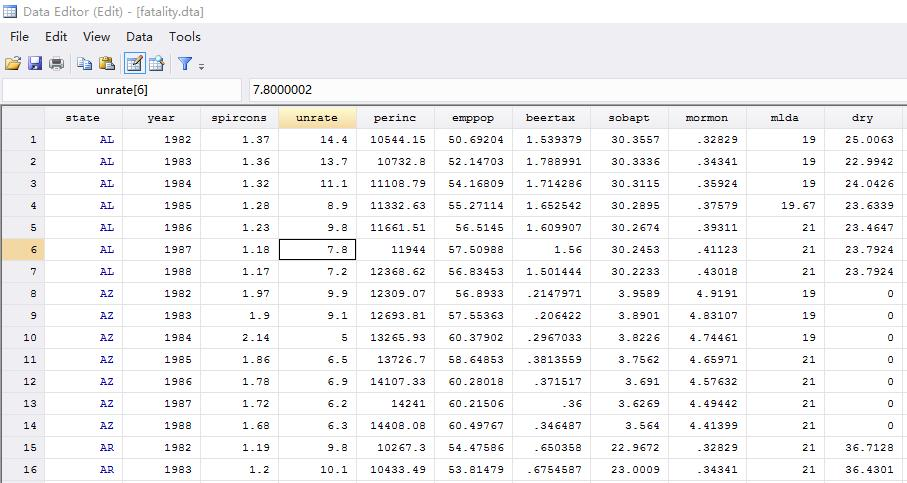
\includegraphics[width=0.7\textwidth]{balancedpanel.jpg}
	\caption{平衡面板}\label{fig:digit}
\end{figure}

(2)\textbf{非平衡面板},即面板中至少有一个时期、一个个体的观测值是缺失的,如图2所示。
\begin{figure}[htbp]
	\centering
	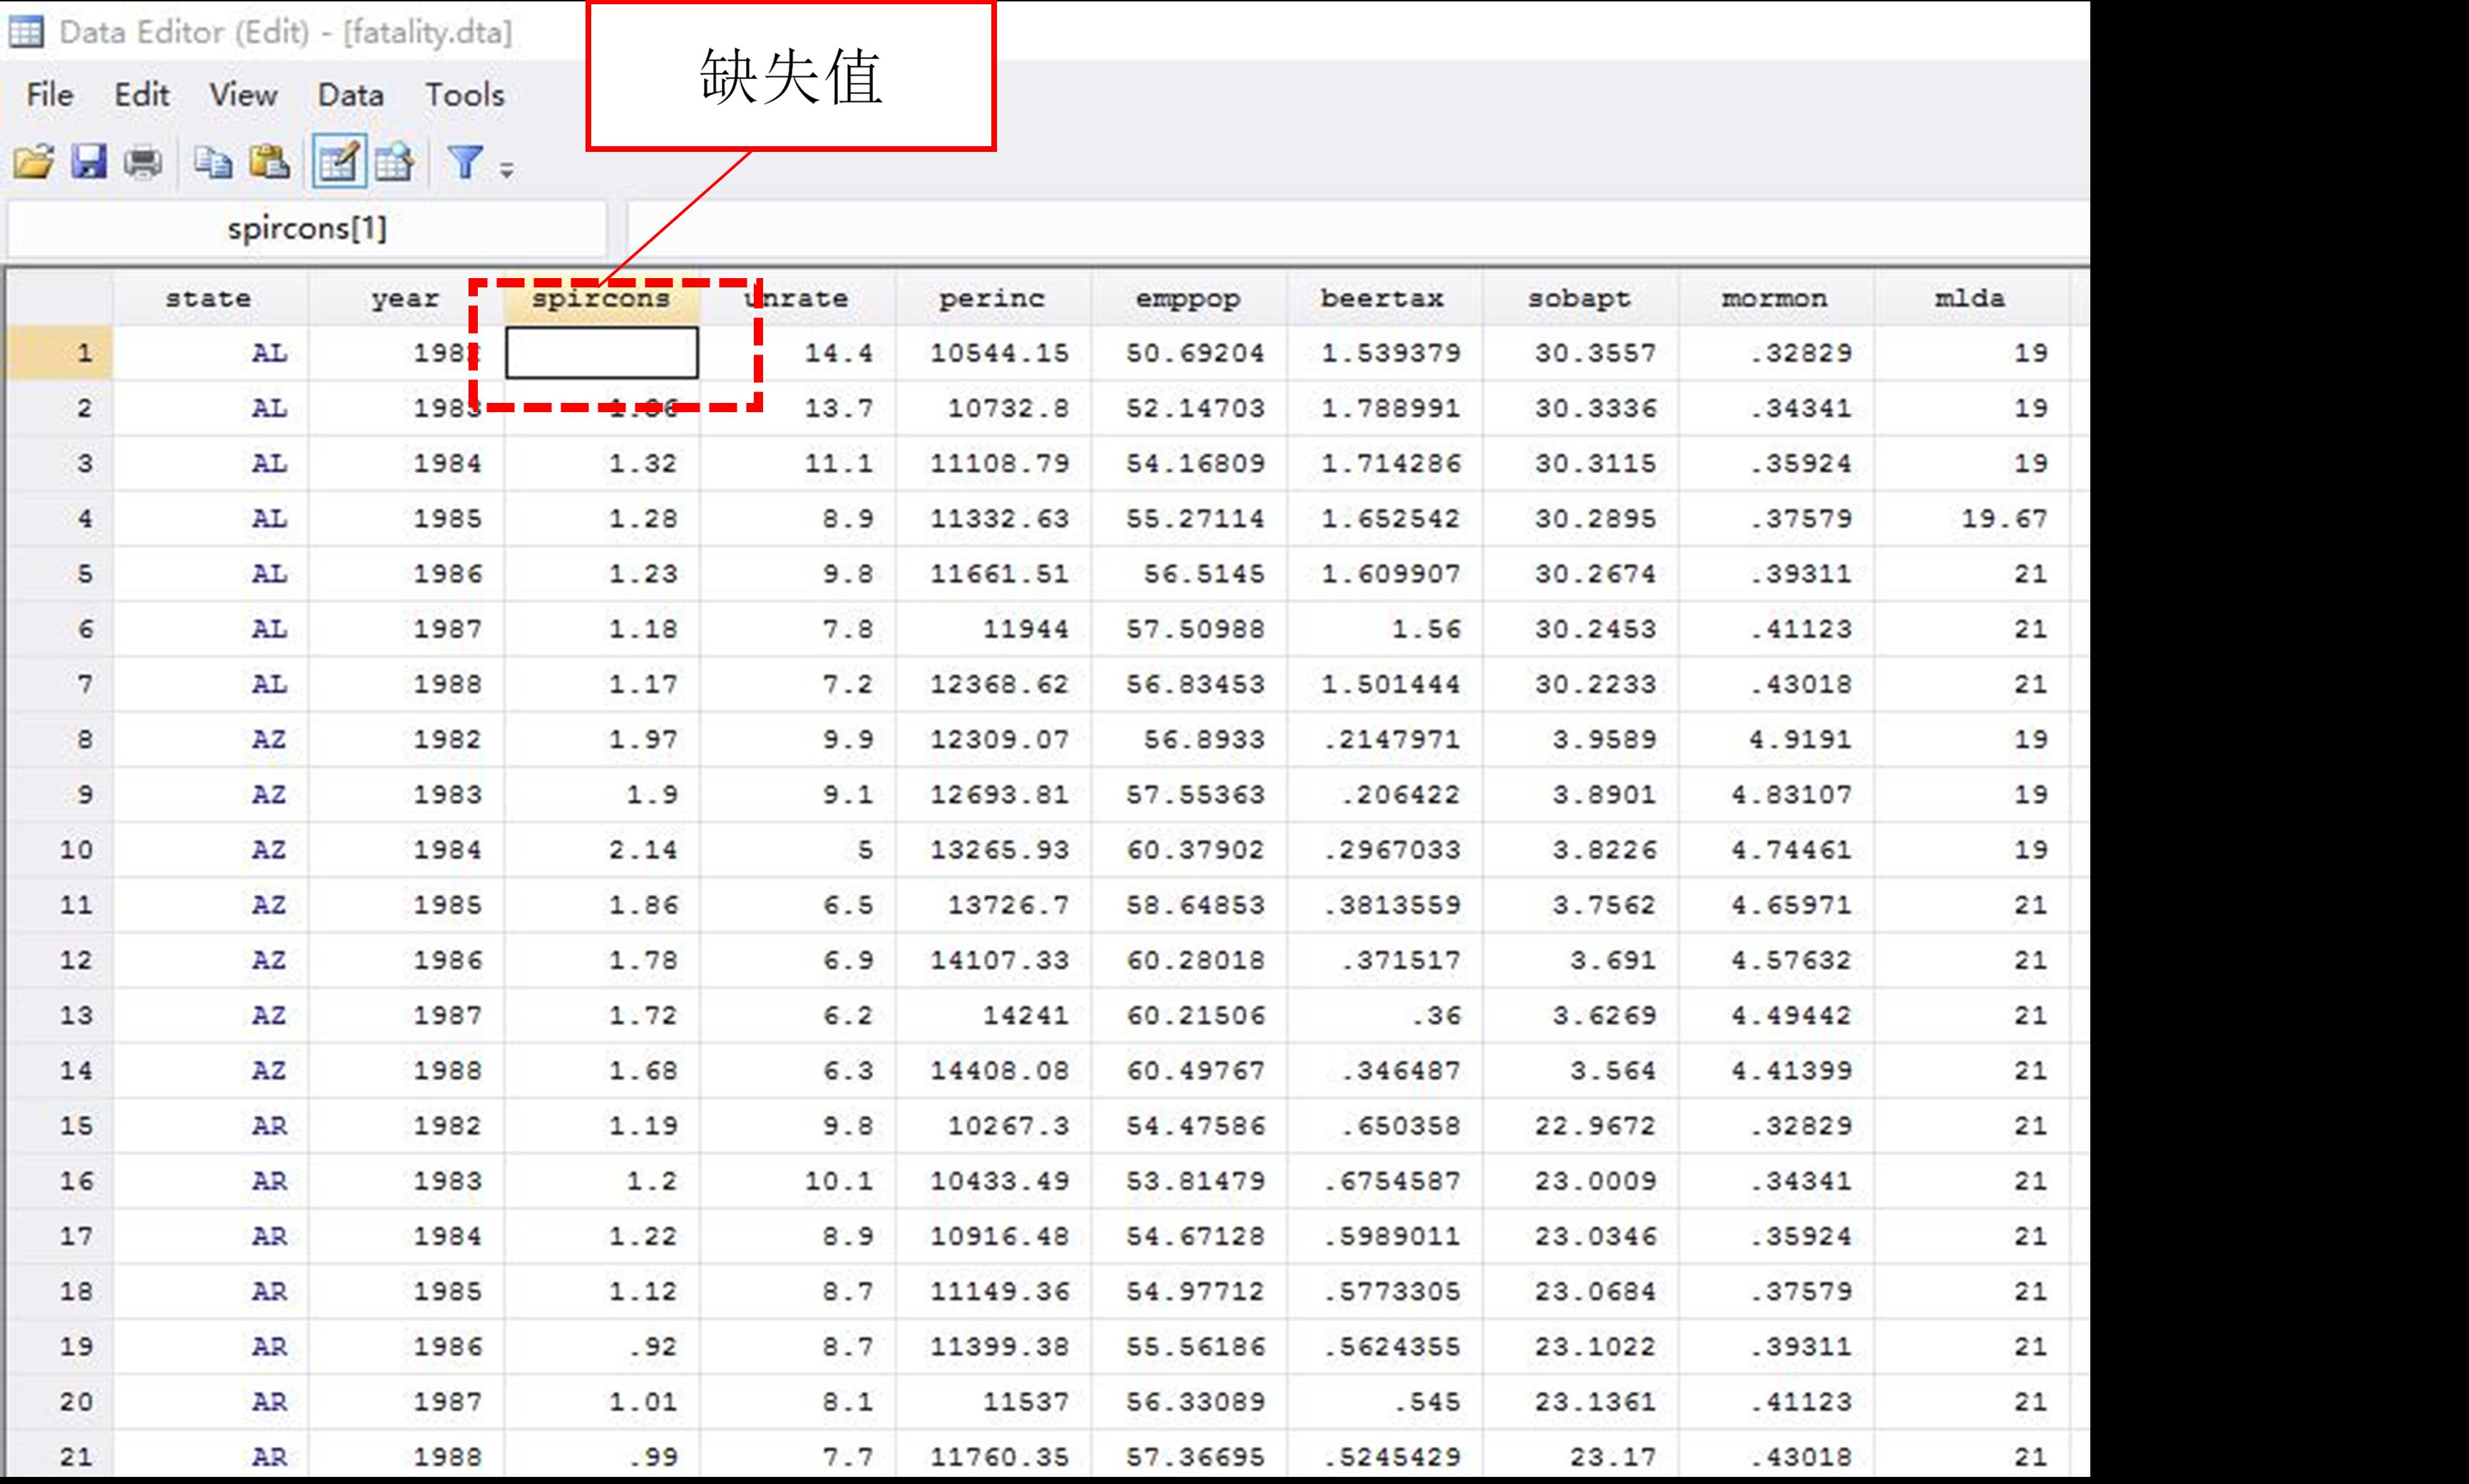
\includegraphics[width=0.7\textwidth]{unbalancedpanel.jpg}
	\caption{非平衡面板}\label{fig:digit}
\end{figure}

在美国,每年将近40000高速交通事故,其中近1/4与醉驾有关。Levitt and Porter(2001)估计在凌晨1点-3点开车的司机中,且达到法定饮酒年龄的,有25\%的司机饮酒后开车上路,他们造成的交通事故至少是没有饮酒的司机的13倍。(注:中国这一情况也非常严重。2009年全国查处酒后驾驶案件31.3万起,其中醉酒驾驶4.2万起。2010年,全国查处醉驾达8.7万起。 2009年1-8月,共发生3206起,造成1302人死亡,其中,酒后驾车肇事2162起,造成893人死亡;醉酒驾车肇事1044起,造成409人死亡。)

下面,我们来看看美国政府实施的抑制醉驾行为的政策到底有多大效果。我们所使用的数据中包含:每年每个州的交通事故数和防止酒驾的政策(包括酒驾法律、酒精税)。交通死亡指标使用\textbf{死亡率(vfrall)——每万人年交通死亡人数}。政策指标是酒精帅,使用\textbf{啤酒税(BeerTax)},且经过1988年通胀处理的实际啤酒税。

图3呈现了1982年交通死亡率与酒精税之间的散点图和拟合线。散点图上的每一个点都代表着1982年给定税率下的死亡率。从图中,可以看出死亡率与税率正相关。回归结果如下

\begin{equation}
	vfrall=2.01+0.15BeerTax(1982年)
\end{equation}

回归结果显示,酒精税的系数为0.15,t统计量为1.12。也就是说,实际酒精税对死亡率的效应为正,但是在10\%的水平下不显著。

\begin{figure}[htbp]
	\centering
	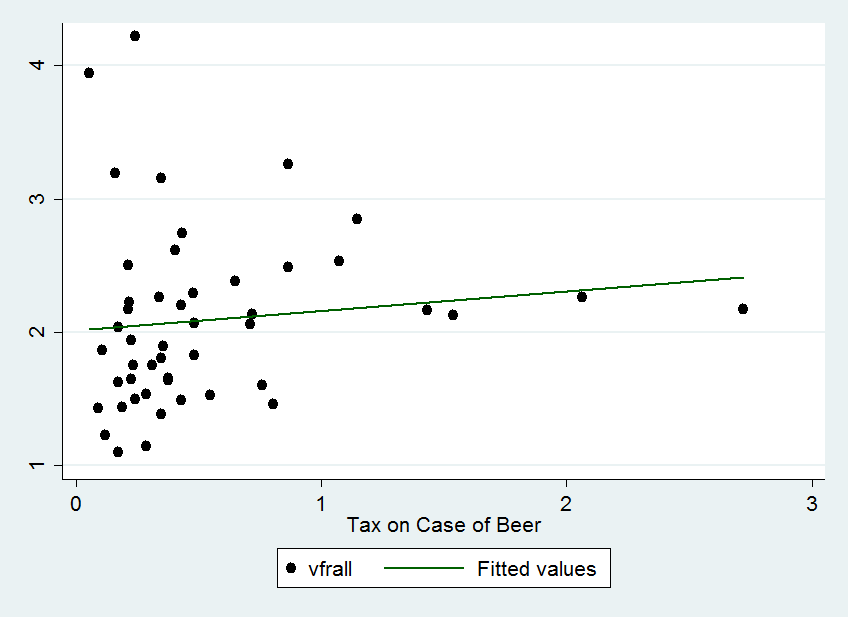
\includegraphics[width=0.7\textwidth]{1982.png}
	\caption{1982年交通死亡率与酒精税}\label{fig:digit}
\end{figure}

从散点图和回归结果来看,这个结果似乎有点奇怪。那么,我们再来看看1988年的结果。其散点图和趋势线如图4所示。回归方程如下
\begin{equation}
	vfrall=1.86+0.44BeerTax(1988年)
\end{equation}

1988年回归结果显示,酒精税的系数为0.44,且t统计量为3.43,也就是说酒精税对死亡率的效应在1\%的水平下显著为正。
\begin{figure}[htbp]
	\centering
	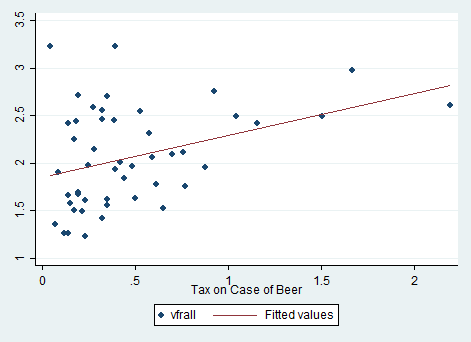
\includegraphics[width=0.7\textwidth]{1988.png}
	\caption{1988年交通死亡率与酒精税}\label{fig:digit}
\end{figure}

虽然,1982年和1988年的估计结果有所差异,但是酒精税的系数均为正。从字面来理解,实际酒精税越高,交通死亡率越高。这似乎与政策设计初衷相悖,也与常识相悖。那么,我们能得出结论:提高酒精税会增加死亡率?

答案显然是否定的!因为上述两个回归结果可能存在很大的遗漏变量偏误。还有许多影响交通死亡率,但又未包含在回归中的因素:汽车质量;公路质量;在农村开车还是在城市;道路上车流密度;对待饮酒和开车的态度等等。这些因素都可能与酒精税有关。如果它们与酒精税相关,就会导致回归结果存在遗漏变量偏误。第四讲为我们提供了一种解决有观测数据的遗漏变量问题的方法——加入其它解释变量(控制变量)。但是,上述有些因素是不可观测的——例如,对饮酒和开车的态度,那怎么办?

如果这些不可观测的遗漏变量不随时间变化,那么,我们可以使用另一种方法来降低遗漏变量偏误。这种方法就是\textbf{固定效应模型}。

\section{固定效应回归}
\subsection{两期“比较”}
在前面的回归中,我们分别对1982年和1988年的截面数据进行回归。那么,我们现在将两年数据结合在一起,形成一个两期的面板数据(n=48,T=2)。这样我们就可以将1988年的被解释变量(死亡率)与1982年进行比较。也就是说,在不可观测因素恒定(在时间维度不变,在个体维度可变)时,我们关注于被解释变量“前”“后”变化。

用$Z_i$表示影响第i个州的交通死亡率的因素,它不随时间变化,因此没有时间下标。那么,这个包含不可观测因素的两期面板数据总体回归线为
\begin{equation}
	vfrall_{it}=\beta_{0}+\beta_{1}BeerTax_{it}+\beta_{2}Z_i+u_{it}
\end{equation}
其中,$u_{it}$表示随机误差项,n=1,⋯⋯,48;T=1982,1988。

因为$Z_i$不随时间变化,也就是说,它在1982年和1988年是一样的。那么,在上述回归方程(3)中,我们可以通过分析1982年-1988年死亡率的变化来消除$Z_i$的影响。从数学形式来看,1982年和1988年的回归方程分别为:
\begin{equation}
	vfrall_{i1982}=\beta_{0}+\beta_{1}BeerTax_{i1982}+\beta_{2}Z_i+u_{i1982}
\end{equation}
\begin{equation}
	vfrall_{i1988}=\beta_{0}+\beta_{1}BeerTax_{i1988}+\beta_{2}Z_i+u_{i1988}
\end{equation}

然后,我们将(5)式减去(4)式来消除$Z_i$的影响:
\begin{equation}
	vfrall_{i1988}-vfrall_{i1982}=\beta_{1}(BeerTax_{i1988}-BeerTax_{i1982})+(u_{i1988}-u_{i1982})
\end{equation}

从(6)式中可以很直观的看出:不可观测因素虽然影响一个州的死亡率,但是它不会在1982年和1988年间变动,因此,它们也不会对这个期间的死亡率变化产生任何影响。

也就说,\textbf{通过分析被解释变量Y与解释变量X的变化量可以消除不随时间变化的不可观测因素,从而消除这种来源的遗漏变量偏误。}

图5呈现了1982-1988两年的散点图和拟合线。图中,dvfrall是1988年vfrall与1982年之差,dbeertax同理。
\begin{figure}[htbp]
	\centering
	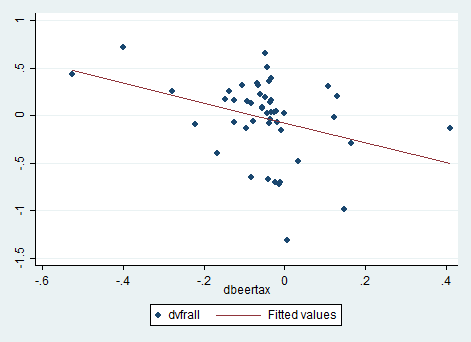
\includegraphics[width=0.7\textwidth]{8288.png}
	\caption{1982、1988年交通死亡率与酒精税}\label{fig:digit}
\end{figure}

回归方程为
\begin{equation}
	vfrall_{i1988}-vfrall_{i1982}=-0.072-1.04(BeerTax_{i1988}-BeerTax_{i1982})
\end{equation}

回归系数为-1.04,且t统计量为-2.93,在1\%的水平显著。与第一节的截面数据结果相比,上述回归结果显示实际酒精税对死亡率有显著地负向影响,也符合经济理论。

上述回归只对包含两期的面板数据可用。而我们所使用的数据集包含7年长度。

\subsection{固定效应回归}

为了消除不随时间变化的不可观测因素带来的影响,可使用固定效应回归。在这种情形下,固定效应回归有n个截距,每个州都有一个。这些截距可以用一个指示变量(二值变量)来表示。而所有不随时间变化的遗漏变量影响都会被这些指示变量吸收。

我们用Y和X来分别表示死亡率和酒精税。那么,我们可以将(3)式写成
\begin{equation}
	Y_{it}=\beta_{0}+\beta_{1}X_{it}+\beta_{2}Z_i+u_{it}
\end{equation}

我们的目的就是估计出$\beta_1$,即酒精税对交通死亡率的影响,且控制不可观测的地区特征$Z_i$。因为$Z_i$只在各州之间变化,而不随时间变化,因此,我们可以令$\alpha_i=\beta_0+\beta_{2}Z_i$。因此,(8)式可以写成:
\begin{equation}
	Y_{it}=\beta_{1}X_{it}+\alpha_i+u_{it}
\end{equation}

(9)式就是\textbf{固定效应模型}。需要注意的是,上述总体回归线的斜率对于每个州都是相同的,但是每个州又对应着不同的截距。因为$\alpha_i$考虑的是个体i的效应,因此,它也被称为\textbf{个体固定效应}。

我们回忆一下二值变量(虚拟变量),上述固定效应回归也可以用二值虚拟变量来表示,例如,如果i=1,令$D_{1i}=1$,否则为0;如果i=2,令$D_{2i}=1$,否则为0;等等。由于有48 个州,因此,设置48个虚拟变量。但是为了避免\textbf{虚拟变量陷阱}(即完全多重共线性),我们要删除一个虚拟变量(任意删除即可)。因此,(9)式可变形为:
\begin{equation}
	Y_{it}=\beta_{0}+\beta_{1}X_{it}+\gamma_2D_{2i}+\cdots+\gamma_nD_{ni}+u_{it}
\end{equation}

由(10)式可知,$\beta_0,\beta_1,\gamma_2,\cdots,\gamma_n$是待估计系数。现在,我们来对比一下(9)式和(10)式:(9)式中,第一个地区的截距为$\alpha_1$,在(10)式中,第一个地区的截距为$\beta_{0}$,因此,$\alpha_1=\beta_{0}$,以此类推第二个第三个等等地区的截距为$\alpha_i=\beta_0+\gamma_i$。也就是说,(9)和(10)是等价的,固定效应模型有两种表达方式。而在这两种表达式中,所有地区的斜率都是一样的,个体固定效应来源于不随时间可变的不可观测地区异质性。

大家可能意识到,上述固定效应模型并没有包含可观测的控制变量。包含其他解释变量的模型同第四讲的多元回归。下面,我们继续讲解固定效应模型的估计和推断。

\textbf{I. 估计和推断}

(9)式中存在不可观测因素$\alpha_i$,因此,不能直接使用OLS。而(10)从理论上讲可以直接使用OLS估计,但是由于其有k+n个参数(k个解释变量的系数,n-1个虚拟变量系数和一个常数项),因此,一旦个体数量非常大,在实践中是很难实施OLS估计(在软件中输入k+n个变量)。幸好,现在有了Stata,它直接可以替我们跑出回归结果。下面,我们稍微看看stata在估计固定效应模型时的工作原理。

\textbf{个体去均值算法}:stata一般会执行两步:

\textbf{第一步,每个变量减去其个体层面的均值。}

例如,在(9)式中,被解释变量Y的个体层面均值为$\overline{Y_i}=\frac{1}{T}\sum_{t=1}^{T}Y_{it}$,解释变量X也同理。然后,用Y减去均值,$Y_{it}-\overline{Y_i}$,X和u也同上。因此,可以得到
\begin{equation}
	\tilde{Y}_{it}=\beta_{1}\tilde{X}_{it}+\tilde{u}_{it}
\end{equation}

\textbf{第二步,估计上述去均值回归方程}。

我们还是利用美国48个州的交通死亡率和酒精税数据来看看上述固定效应回归结果:
\begin{equation}
	\tilde{vfrall}_{it}=-0.66\tilde{BeerTax}_{it}(去均值结果)
\end{equation}

\begin{equation}
	vfrall_{it}=-0.66BeerTax_{it}+\alpha_i
\end{equation}

上文我们提到过,上述个体固定效应模型也遗漏了一些变量,除了可观测的变量之外,还有一个重要的遗漏变量就是不可观测的不随地区变化的因素。

\textbf{II. 时间固定效应}

类似于个体固定效应,时间固定效应是不随个体变,而随时间变化的因素。我们用$S_t$表示,那么,只包含时间固定效应的模型为
\begin{equation}
	Y_{it}=\beta_{0}+\beta_{1}X_{it}+\beta_{3}S_t+u_{it}
\end{equation}

与上述个体固定效应同理,由于$S_t$不随地区变化,只随时间变化,因此,令$\lambda_t=\beta_{0}+\beta_{3}S_t$。那么,(14)式可以变为
\begin{equation}
	Y_{it}=\beta_{1}X_{it}+\lambda_t+u_{it}
\end{equation}

同理,每一个时期都有一个截距,截距$\lambda_t$就是时间t对被解释变量Y的效应,也被称为\textbf{时间固定效应}。

同样的,时间固定效应模型也有两种表达方式:一种是时间虚拟变量;另一种是(15)式。
\begin{equation}
	vfrall_{it}=-0.02BeerTax_{it}+\lambda_t
\end{equation}
加入时间固定效应之后,上述回归结果并不显著。

下面,我们来看看同时加入个体固定效应和时间固定效应的模型:
\begin{equation}
	Y_{it}=\beta_{1}X_{it}+\alpha_i+\lambda_t+u_{it}
\end{equation}

与个体固定效应的算法相同,时间固定效应和双向固定效应的算法也可以采用“去均值算法”。

首先,Y和X分别减去其个体层面均值和时间层面均值;

然后,用两次差分之后的去均值变量进行回归,用OLS估计系数。

另一种方式,就是我们常用的Y和X只减去个体层面的均值,然后设立时间虚拟变量,用\textbf{fe}命令进行回归。用这种方式得到的回归结果为
\begin{equation}
	Y_{it}=-0.64X_{it}+\alpha_i+\lambda_t+u_{it}
\end{equation}
回归结果在10\%的水平下显著。

\textbf{注:一般来讲,面板数据都需要控制个体固定效应和时间固定效应,因为这可以消除不可观测的随时间可变不随个体变化的因素或者不随个体变化随时间变化的因素所引起的遗漏变量偏误。在使用家庭(企业)层面、省(市县)层面的数据后,还要同时控制家庭固定效应、省固定效应和时间固定效应。}

\textbf{III. 聚类标准误}

在面板数据模型中,我们假设个体之间是独立的,但是在个体层面内部,由于存在不同时间的观测值,因此它们不一定独立。这就可能存在个体内部的自相关或者序列相关问题。这就意味着误差项u可能也存在自相关问题。此时,截面数据回归的异方差稳健标准误就不再有效。为了消除面板数据回归中误差项自相关问题,我们要使用异方差-自相关一致性(HAC)标准误,也就是\textbf{聚类标准误}。我们上述的回归结果都是使用的聚类标准误。

\textbf{注:在面板数据回归中,一定要使用“聚类标准误”,也就是个体层面的聚类}

\subsection{例子}
\begin{figure}[htbp]
	\centering
	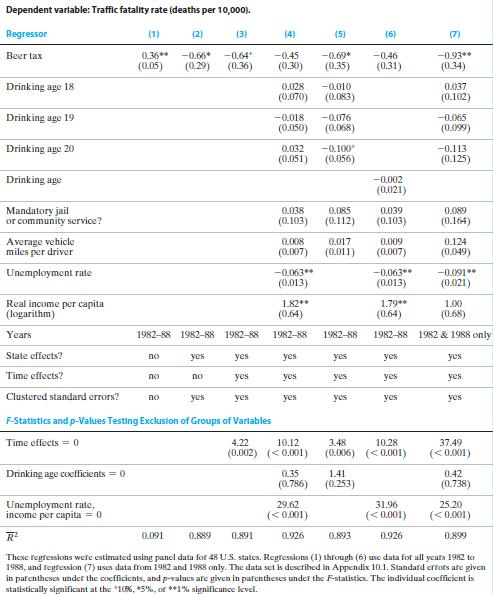
\includegraphics[width=0.7\textwidth]{results.jpg}
	\caption{交通死亡率与酒精税}\label{fig:digit}
\end{figure}
	
	\chapter{工具变量法}
	正如第五讲所述,一项经验研究可能存在的主要问题:遗漏变量偏误、变量测量误差、反向因果、模型设定错误、样本选择偏误、异方差和序列相关。第四讲和第六讲分别呈现了消除某种遗漏变量偏误的方法——多元回归和面板数据模型。多元回归应对遗漏变量数据可用情形;面板数据模型引入个体固定效应和时间固定效应来消除遗漏变量数据不可用,且截面或时间单一维度变化时的遗漏变量偏误。
	
	一来,上述两种解决方法均相当于在回归模型中增加核心解释变量($X_{it}$) 以外的自变量($Z_{it},\alpha{_i},\gamma{_t}$);二来,变量测量误差和反向因果所引起的问题,并不能由多元回归和面板数据模型直接解决。那么,除此之外,还有没有其他方法来解决遗漏变量偏误、变量测量误差、反向因果问题呢?
	
	\textbf{工具变量(Instrumental variables,IV)回归}就是获得X与u相关的总体回归函数未知系数一致估计量的一种常用方法。\textbf{IV的核心思想:把核心解释变量X 的变动分解成两个部分:一个部分与误差项u相关,另一个部分与误差项u不相关。如果我们有资料、数据、信息来分离出第二部分,那么,我们就可以只关注于误差项无关的第二部分,丢弃引起OLS估计偏误的第一部分。}这些表征X变动,且与u不相关的数据信息可能来源于一个或多个其他变量,这些变量就称为\textbf{工具变量(IV)}。 如字面意思,这些变量被作为工具来分离出X中与u无关的部分,从而确保回归系数估计量具有一致性。
	
	下面,详细阐述工具变量法的作用原理及其应用。
	
	\section{一元回归与单工具变量}
	如第五讲所述,引起X与u相关的原因可能是遗漏变量、变量误差、反向因果。无论什么原因,如果我们有一个有效的工具变量$I$,那么,我们就可以利用工具变量估计量来估计出X对Y的效应。总回归模型为
	\begin{equation}
		Y_i=\beta_0+\beta_1X_i+u_i
	\end{equation}
	
	如果$corr(X_i,u_i)\neq0$,OLS估计量就是非一致的。我们就可以用工具变量$I_i$ 来分离出$X_i$中与$u_i$无关的部分。
	
	依据是否与误差项u相关,可以把变量划分成\textbf{内生变量}和\textbf{外生变量},前者与误差项相关,后者与误差项无关。这两个名字可以追溯至多方程模型,即“内生变量”由模型内决定,“外生变量”由模型外决定。这两个变量在后面的DSGE模型中还会见到。
	
	有效的工具变量必须同时满足两个条件:
	
	\textbf{(1)工具变量相关性条件:$corr(I_i,X_i)\neq0$}
	
	\textbf{(2)工具变量外生性条件:$corr(I_i,u_i)=0$}
	
	工具变量相关性表明一个工具变量的变动与X的变动相关。工具变量外生性表明工具变量抓住了X中外生变化的部分。这两个条件对于工具变量回归非常重要。
	
	\subsection{两阶段最小二乘TSLS}
	\textbf{两阶段最小二乘(TSLS)}是用来估计IV估计量的方法。正如该方法的名字所述,IV估计量是通过两个阶段计算出来的。
	
	\textbf{第一阶段},把X分解成两个部分:可能与误差项相关的部分和与误差项无关的第二部分。
	
	具体来说,第一阶段用X对工具变量I回归:
	\begin{equation}
		X_i=\pi_0+\pi_1I_i+v_i
	\end{equation}
	
	公式(2)就把X分解成:$v_i$和$\pi_0+\pi_1I_i$。由于$I_i$是外生的,因此,$\pi_0+\pi_1I_i$与$u_i$无关,而剩下的$v_i$与$u_i$相关。据此,我们可以用样本数据估计出$\hat{\pi}_0,\hat{\pi}_1$,然后从OLS回归中得到X的预测值$\hat{X}_i=\hat{\pi}_0+\hat{\pi}_1I_i$。
	
	\textbf{第二阶段},利用与误差项无关的第二部分估计$\beta_1$。也就是说,$Y_i$对$\hat{X}_i$回归,利用OLS估计系数,进而得到TSLS估计量,$\hat{\beta}_0^{TSLS}、\hat{\beta}_1^{TSLS}$
	
	\textbf{I. 香烟需求}
	
	下面,我们使用美国48个州1985-1995年的香烟销售相关数据。我们用这些数据来估计香烟的需求弹性。工具变量——销售税:来自于一般销售税中对烟草征收的税。香烟消费量,$Q_i^{cig}$,是第i 个州人均消费香烟包数。价格,$P_i^{cig}$,含税实际平均价格。
	
	在进行TSLS之前,大家首先要关注工具变量是否有效,也就说,我们选择的工具变量是否满足前面的两个条件——相关性和外生性。后面,我们会详细给出如何通过统计工具来检验工具变量的有效性。在此之前,我们先来看看这销售税是否能作为一个有效的工具变量。
	
	首先,工具变量相关性。销售税越高,香烟的税后价格也会越高,那么,销售税与香烟价格具有相关性;
	
	其次,工具变量外生性。一般来说,销售税在各州之间是不同的,但是这种差异并不主要由香烟需求决定,而是由于政治考虑。因此,我们也可以认为销售税是外生的。
	
	根据上述TSLS的两个阶段,用1995年的48个州的数据,我们先来看看第一阶段回归:
	\begin{equation}
		\tilde{ln(P_i^{cig})}=4.62+0.31SalesTax_i
	\end{equation}
	回归结果均在1\%下显著,而且如经济理论预测的,销售税越高,税后价格就越高。回归方程的$R^2=0.47$,也就睡说,销售税变化解释了47\%的香烟价格变动。
	
	在第二阶段中,用$ln(Q_i^{cig})$对$\tilde{ln(P_i^{cig})}$来进行回归。回归结果是
	\begin{equation}
		\tilde{ln(Q_i^{cig})}=9.72-1.08\tilde{ln(P_i^{cig})}
	\end{equation}
	也就是说,第一阶段的预测值$\tilde{ln(P_i^{cig})}$,被用作第二阶段的回归量。但是,软件中输出的结果是$ln(P_i^{cig})$,而不是$\tilde{ln(P_i^{cig})}$。因此,TSLS估计为
	\begin{equation}
		\tilde{ln(Q_i^{cig})}=9.72-1.08ln(P_i^{cig})
	\end{equation}
	
	TSLS的估计结果显示,香烟的需求弹性是富有弹性的:价格提高1\%,香烟需求量下降1.08\%。
	
	从第四、五、六讲我们可以知道,上述估计结果可能存在遗漏变量偏误。
	
	\section{IV回归}
	在一般化的IV回归模型中,主要包括四种类型的变量:被解释变量Y;内生解释变量X;外生解释变量W;工具变量I。一般来说,可能存在多个内生解释变量,多个外生解释变量和多个工具变量。
	
	回归系数是\textbf{恰好识别},如果工具变量与内生解释变量一样多;
	
	回归系数是\textbf{过度识别},如果工具变量比内生解释变量还多;
	
	回归系数是\textbf{识别不足},如果工具变量比内生解释变量还少;
	
	需要注意的是:\textbf{IV回归中,至少要有与内生回归因子(内生解释变量)一样多的工具变量。}
	
	在IV中包含外生变量或控制变量是为了确保工具变量与误差项不相关。
	
	\textbf{【小贴士】}(以下内容来源于“SociologyOfDrink"微信公众号2018-01-05期张友浪”控制变量是否越多越好)控制变量一般没有因果解释,但控制变量又很重要,那么,怎么选择控制变量呢?一般来说我们只需控制能够同时影响解释变量和被解释变量的变量(confounder)。但是,我们在投稿时经常会收到审稿人的意见,说这个没有控制那个也没有控制。或者自己有意无意的在回归中包含了过多的控制变量。而控制变量过多往往会造成模型损失自由度,模型不够简洁,模型过度拟合,甚至会让我们得出错误的结论。这些问题在小样本回归中尤为严重。因此,我们在回归时,真正要考虑的是,什么样的变量不需要被控制?
	
	根据某一备选变量在因果关系中的位置,可以分以下几种情况讨论:
	
	(1)既不影响解释变量,也不影响被解释变量。很多社会经济变量不仅仅因为常见,而被人们要求加入模型。但如果没有可信的理论来支撑对解释变量和被解释变量的影响的话,不应将其纳入模型;
	
	(2)只影响解释变量的变量。这类变量与关键解释变量没有直接影响,不影响我们对解释变量影响的估计,当然无需纳入模型中控制;
	
	(3)只影响被解释变量的变量。这类变量与关键解释变量不存在理论上的相关性,不会造成遗漏变量偏误,无需控制;
	
	(4)被解释变量影响,又影响解释变量的变量,即中介变量(mediator)。考虑到我们的关键解释变量对被解释变量的影响往往是通过一个或多个渠道(因果链条可无限细分),这时就要分两种情况做决定:如果该中介变量处在我么假设的因果链条中,那就应该将其去掉,因为加入这个变量会让解释变量的影响从全部影响减弱为直接影响,而间接影响则被中介变量吸收,从而削弱了我们对解释变量整体效应的估计;如果该中介变量并不处在我们假设的因果链条中,那就应该保留,这时对自变量影响的估计就会自动排除竞争性解释的影响,有助于提高估计结果的可信度;
	
	(5)当然,有时候,会遇到审稿人搞不清因果关系,坚持要求加入某个变量来控制。考虑到硬怼审稿人没什么好下场,因此建议,审稿人说什么就是什么,听从他们的意见,控制审稿意见要求的变量。
	
	\subsection{TSLS}
	
	当回归方程中只有一个内生解释变量X和多个外生变量时,回归方程为
	\begin{equation}
		Y_i=\beta_0+\beta_1X_i+\beta_2W_{1i}+\cdots+\beta_{1+r}W_{ri}+u_i
	\end{equation}
	
	如前所述,X可能与误差项相关,W则不与误差项相关。
	
	根据前文TSLS的两个阶段。在\textbf{第一阶段}中,用X与所有的外生变量——外生解释变量W和工具变量I进行回归。
	\begin{equation}
		X_i=\pi_0+\pi_1I_{1i}+\cdots+\pi_mI_{mi}+\pi_{m+1}W_{1i}+\cdots+\pi_{m+r}W_{ri}+v_i
	\end{equation}
	
	在TSLS的\textbf{第二阶段},先用(7)式估计的$\tilde{X}_i$来替代(6)式中的X,然后进行OLS估计。由此,得到的$\beta_0,\beta_1,\cdots$就是TSLS的估计量。
	
	\textbf{【小贴士】}
	
	1、在进行第一阶段回归时,除了工具变量外,所有的外生变量(或控制变量)都需要包含在其中。而第二阶段回归也需要包含这些外生变量。
	
	2、当有多个内生解释变量时,第一阶段的工具变量回归是每个内生解释变量分别与它对应的工具变量进行回归,然后再将所有的估计值放入第二阶段回归中得到TSLS估计量。
	
	\subsection{例子:香烟需求}
	
	在第一节的香烟需求例子中,我们只估计了单变量。但是这可能会存在遗漏变量偏误,例如,州的收入水平可能既影响香烟需求,也影响销售税。那么,这还会使得工具变量外生性条件不被满足。因此,下面,我们在回归中包含州的收入水平。TSLS的估计结果为
	\begin{equation}
		\tilde{ln(Q_i^{cig})}=9.43-1.14ln(P_i^{cig})+0.21ln(Inc_i)
	\end{equation}
	
	上面的回归系数的标准误为0.37,是恰好识别,也就是说单一内生解释变量对应单一工具变量。除了销售税作为工具变量之外,还可以使用州的烟草特种税。因此,这种税是第二种可能的工具变量。烟草特种税(CigTax)提高会增加香烟的价格,因此满足相关性条件,如果它与误差项无关,那么它也满足外生性条件。下面,我们用两个工具变量来重新进行TSLS 估计,估计结果如下:
	\begin{equation}
		\tilde{ln(Q_i^{cig})}=9.89-1.28ln(P_i^{cig})+0.28ln(Inc_i)
	\end{equation}
	上述两个IV的估计系数标准误为0.25,比较(9)式和(8)式的标准误,我们可以看出,(9)的标准误比(8)下降了三分之一左右。这是因为(9)式利用了更多的信息,两个IV解释了更大的价格变动。
	
	那么,上述IV估计结果可信吗?很遗憾,我们不能立马回答上述问题,因为可信度依赖于IV是否有效。因此,IV有效的两个条件——相关性和外生性就必须要被检验。
	
	\section{如何检验IV的有效性}
	
	我们仍然用美国48个州的1985-1995年的香烟销售数据。我们来估计长期价格弹性,因此用十年的的数据来进行回归,例如,我们用香烟销售量的对数之差$ln(Q_{i,1995}^{cig})-ln(Q_{i,1985}^{cig})$,价格的对数之差$ln(P_{i,1995}^{cig})-ln(P_{i,1985}^{cig})$和收入的对数之差$ln(Inc_{i,1995}^{cig})-ln(Inc_{i,1985}^{cig})$。两个工具变量是$SalsTax_{i,1995}-SalsTax_{i,1985}$,$CigTax_{i,1995}-CigTax_{i,1985}$。
	
	结果呈现在图1中,每一列都是不同的回归,都是用TSLS估计量,唯一的差别是工具变量不同。第一列是只包含销售税这个工具变量;第二列是只包含烟草税这个工具变量;第三列是包含两个工具变量。从图1中的结果可以看出,三列结果的第一行均在5\%水平下显著为负。但这个结果可信吗?这依赖于我们使用的工具变量是否有效。
	
	
	\begin{figure}[htbp]
		\centering
		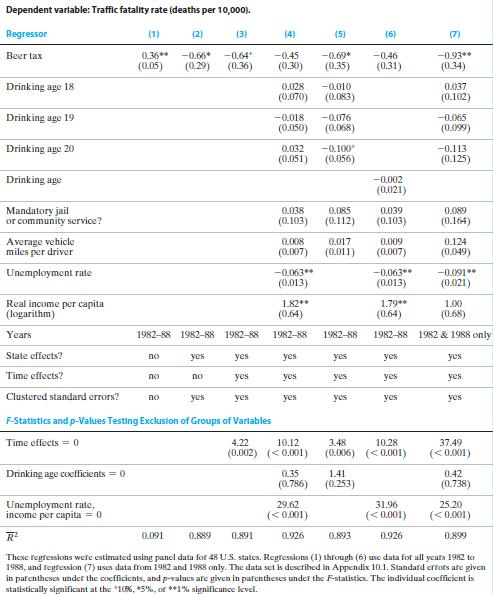
\includegraphics[width=1\textwidth]{results.jpg}
		\caption{香烟需求}\label{fig:digit}
	\end{figure}
	
	
	
	(I)我们首先来看看,\textbf{工具变量的相关性}。
	
	工具变量相关性的作用类似于“样本规模的作用”。因为工具变量与内生解释变量越相关,说明IV回归中包含X的信息越多,TSLS估计量越准确,这就类似与样本量越大,估计结果 越准确。
	
	工具变量解释X变动的部分较少时,这种工具变量成为\textbf{弱工具变量}。在上面的例子中,如果选取香烟生产企业到州的距离作为工具变量,这可能就是一个弱工具变量。尽管这个距离越远,香烟的销售价格越高,但是香烟较轻,运输成本可能在其价格中并不是主要组成部分,因此,距离的变动很可能只能解释价格变动中的一小部分。因此,生产距离可能就是一个弱工具变量。那么,如何检验一个工具变量是否是弱工具变量?如果是弱工具变量,我们应该怎么处理?
	
	上面已经说过,工具变量的作用类似于大样本的作用。如果存在弱工具变量问题,正态分布就不是TSLS估计量抽样分布的良好近似,那么,TSLS估计量就不再可信。那么,工具变量相关性程度有多大才是一个良好的分布近似呢?这个答案很复杂,但是幸运的是,我们在实践中有一些经验规则可用:
	
	\textbf{检验弱工具变量的经验规则:}当只有一个内生解释变量时,检验弱工具变量的方法就是计算TSLS第一阶段的F统计量。\textbf{第一阶段F统计量}为包含在工具变量中的信息提供了一个不错的测量指标:包含的信息越多,F统计量越大。\textbf{经验规则是;如果第一阶段F统计量大于10,不存在弱工具变量;如果小于10,可能就是弱工具变量。}
	
	我们从图1中可以看到,三个TSLS的回归结果中,一阶段F统计量分别为33.7,107.2和88.6,因此,我们选择的工具变量不是弱工具变量。
	
	那如果上面的一阶段F统计量小于10,\textbf{也就是说存在弱工具变量,我们该怎么办呢?}
	
	如果存在弱工具变量,且有一些工具变量比另一些更弱。那么,就应该舍弃那些最弱的工具变量。当我们放弃一些弱工具变量时,TSLS估计量的标准误可能会变大,但是       \textbf{请记住“原始标准误没有任何意义”!}
	
	但是,如果系数恰好识别,也就是一个内生解释变量,只有一个工具变量,且是弱工具变量时,我们就不能舍弃这个弱工具变量了。即使在过度识别时,没有足够的强工具变量来取得识别效果,舍弃弱工具变量也不会有任何帮助。这种情况下,我们可以干两件事:
	
	(1)去寻找其他的更强的工具变量。说起来容易,做起来难!这需要我们对所研究的问题有足够的认识,并且能重写设计和收集相关数据。
	
	(2)仍然使用弱工具变量,但是估计方法不用TSLS,而用其他估计方法,例如有限信息极大似然(LIML)估计量。
	
	(II)\textbf{工具变量外生性}
	
	如果有一个内生解释变量,多个工具变量,那么,我们可以计算出多个TSLS估计量(每个工具变量计算一个)。假设有两个工具变量,那么,我们计算的两个TSLS估计量不同。但是如果两个工具变量都是外生的,那么,它们会十分接近。如果我们估计的两个TSLS估计量差异非常大,那么,我们就要非常警觉:要么其中一个工具变量不是外生的,要么两个都不是外生的。在过度识别情形下,\textbf{过度识别限制检验(J统计量)}就是在对多个工具变量TSLS估计量进行比较。
	
	总之,在过度识别情形下,我们能计算出多个TSLS估计量,然后比较它们是否接近,即通过stata计算出\textbf{J统计量}。如果是精确识别情形,我们就不能比较,实际上,这个时候的J统计量为0。
	
	从图1中可以看出,(1)列和(2)列只有一个工具变量,因此,不存在J统计量。而在第(3)列中,有两个工具变量,是过度识别情形,因此,可以计算J统计量,其结果为4.93,它服从卡方分布,5\%的临界值为3.84,因此,它在5\%的水平下拒绝两个工具变量都是外生的假设。这是因为两个工具变量的TSLS估计量差异很大。J统计量拒绝原假设意味着第(3)列的估计是基于无效的IV估计,因为IV外生性条件不满足。那么,这是否就意味着我们估计的三个结果都不行呢?J统计量拒绝原假设只意味着两个工具变量中至少有一个是内生的,那么,我们可以推断:第一,销售税是外生的,烟草税不是,那么,(1)中的结果就是可靠的;第二,烟草税是外生的,销售税不是,那么,(2)中的结果是可靠的;第三,两个都不是外生的,那么,三个结果在统计意义上都可靠。
	
	\textbf{千万要记住:统计证据并不能告诉我们哪一种可能是正确的,因此这就需要我们根据我们的经验以及经济理论去argue。}
	
	
   \section{异质性处理效应的IV估计量}



	\section{哪里去寻找有效的工具变量呢?}
	
	在实践中,IV回归最难的就是找到有效的工具变量。虽然如此,但是还是有两种指导性的方法:
	
	(I)遵循经济理论来找工具变量。例如,IV回归的发明者P. Wright(1928)通过他对农业市场的理解,使他认识到所寻找的IV不是使需求曲线移动,而是使供给曲线移动,因此,他就想到用农业地区的天气条件作为有效IV。经济理论法最成功的领域就是金融经济学。在这个领域,有一些投资者行为的经济模型通常是非线性的,此时,不能使用IV估计。因此,将IV方法扩展到非线性模型时,这种扩展方法就是广义矩估计(GMM)。但是经济理论太抽象,并不总是能找到一个有效的IV。
	
	(II)构造工具变量。从这种视角出发,我们要去寻找那些引起内生解释变量变化的随机事件,从这些随机事件中剥离出X变动的外生冲击。
	
	“连享会”微信公众号上有一篇关于寻找工具变量的推文(\href{https://www.lianxh.cn/news/946348365bb2d.html}{秦范 (2021)})中写道:
	
	工具变量要满足外生性和相关性两个条件,因此寻找工具变量也一般从满足这两个条件出发。常见的寻找工具变量一般思路如下:
	
	\begin{itemize}
		\item 气候、地理等自然因素:降雨等气象因素、地势等地理条件是高度随机的,但也会影响某些经济社会过程,从而能够满足外生性和相关性;
			\item 历史因素:过去的历史事件一般与当今的社会经济结果无关;
			\item 生理现象:生育双胞胎等现象具有较强的随机性。
		\item 	使用更高层级的变量作为低层级变量的工具变量:比如,研究个体金融知识与创业选择时,创业概率与金融知识存在反向因果关系,因而金融知识是内生变量。为了克服内生性,作者选用同一个社区其它居民的金融知识平均水平作为个体金融知识的工具变量。但从这一角度寻找工具变量,往往不能完全保证外生性;
			\item 内生变量的滞后项。
	\end{itemize}
	
	
	\section{Stata命令}
	
	我们再来看两个两个例子:1、同质处理效应——教育年限对收入的影响;2、异质性处理效应——富尔顿渔业市场的售价对营业额的影响。
	
	\subsection{教育年限的工具变量:城市是否存在大学}
	
	数据和代码来源于Scott Cunningham(2021):“Causal Inference:The Mixtape”的第七章。而教育年限对收入的影响则是Card(1995)研究的劳动经济学问题。作者设立了一个回归:
	
	\begin{equation}
		Y_i = \alpha +\delta S_i + \gamma X_i +\epsilon_i
	\end{equation}
	
	其中,$Y$表示收入对数,S是受教育年限,X是外生协变量矩阵,$\epsilon$是误差项——包含不可观测的个人能力,由于能力与受教育年限相关,这就意味着上述估计结果是有偏的。为了解决这个问题,Card(1995)提出用工具变量策略,即用“城市是否存在大学”这个虚拟变量来作为受教育年限的工具变量。
	
	还记得前面的内容反复提到的“自问”吗?此时,我们仍要首先啪啪脑门(注意,只是轻拍,千万不要抓,抓会掉头发的),自问一下:为什么城市是否存在大学这个虚拟变量可以作为受教育年限S的工具变量呢?我能想到的第一个原因就是:父母想把我们留在身边读书。但是,这个答案是否仍然有点牵强。我们再想想,我是武汉人,在武汉上的大学,那个时候家境一般,父母供三个孩子读书,负担还是挺重的,所以在武汉读书也许会减轻家里的学费、生活费、交通费等等负担,因为我就住在武汉。确实,武汉存在大学,所以可能会通过降低了我们继续受教育的成本,进而提高了我们继续读书的可能性——可能增加了受教育年限S。好了,那么,我们就姑且先用这个虚拟变量作为IV来估计上述回归方程的OLS估计量和2SLS估计量,并进行比较。
	
	\begin{lstlisting}
		* Stata代码
		
		use /Users/xuwenli/OneDrive/DSGE建模及软件编程/教学大纲与讲稿/应用计量    ///
		经济学讲稿/应用计量经济学讲稿与code/data/card.dta,clear
		
		* 教育年限对工资对数的OLS估计
		
		reg lwage  educ  exper black south married smsa
		
		* 用“城市是否存在大学”作为受教育年限的工具变量跑2SLS估计
		
		ivregress 2sls lwage (educ=nearc4) exper black south married smsa, first 
		
		* 大学和城市变量以及所有协变量对受教育年限的第一阶段回归
		
		reg educ nearc4 exper black south married smsa
		
		* 第一阶段回归的F统计量:IV的排除性
		
		test nearc4
	\end{lstlisting}
	
	表7.1 给出了上述估计结果。从表中可以看出,第二列OLS的回归结果显示受教育年限每增加一年,工资对数会提高7.1\%左右,且在1\%的置信水平下显著。第三例2SLS的回归结果显示,受教育年限每增加一年,工资对数提高12.4\%左右,这个估计结果比OLS还要大。
	
	下面,我们来看看第一阶段的回归结果,列示在“第一阶段IV回归”的“College in the county”行中。结果显示,城市存在大学可以增加0.327年的受教育年限,而且在1\%的水平下显著。F统计量也超过了15,这意味着并不存在弱工具变量问题。
	
	\begin{table}[htbp]\centering
		\scriptsize
		\caption{受教育年限对收入对数的OLS and 2SLS回归}
		\label{2sls_1}
		\begin{center}
			\begin{threeparttable}
				\begin{tabular}{l*{2}{c}}
					\toprule
					\multicolumn{1}{l}{\textbf{因变量}}&
					\multicolumn{2}{c}{\textbf{Log wage}}\\
					\multicolumn{1}{c}{}&
					\multicolumn{1}{c}{OLS}&
					\multicolumn{1}{c}{2SLS}\\
					\midrule
					educ                &       0.071***&       0.124** \\
					&     (0.003)   &     (0.050)   \\
					exper               &       0.034***&       0.056***\\
					&     (0.002)   &     (0.020)   \\
					black               &      -0.166***&      -0.116** \\
					&     (0.018)   &     (0.051)   \\
					south               &      -0.132***&      -0.113***\\
					&     (0.015)   &     (0.023)   \\
					married             &      -0.036***&      -0.032***\\
					&     (0.003)   &     (0.005)   \\
					smsa                &       0.176***&       0.148***\\
					&     (0.015)   &     (0.031)   \\
					\\
					\midrule
					\multicolumn{1}{c}{第一阶段IV回归}\\
					College in the county&               &       0.327***\\
					Robust standard error &               &       0.082   \\
					F statistic for IV in first stage&               &      15.767   \\
					Anderson-Rubin test &               &           .   \\
					N                   &       3,003   &       3,003   \\
					Mean Dependent Variable&       6.262   &       6.262   \\
					Std. Dev. Dependent Variable&       0.444   &       0.444   \\
					\bottomrule
				\end{tabular}
				\begin{tablenotes}
					\tiny
					\item 括号里为标准误,* p$<$0.10, ** p$<$0.05, *** p$<$0.01
				\end{tablenotes}
			\end{threeparttable}
		\end{center}
	\end{table}
	
	在理解受教育年限的收入效应时,有几个问题需要特别注意:我们用城市是否有大学来作为受教育年限的IV,这就意味着我们选择的组群的行为(是否接受教育)会受到IV的影响。换言之,在总体样本中,应该会有部分学生总会去读大学,还有一部分学者就是不想去读大学,这两部分人的教育决策并不受到城市是否有大学的影响。但是,还有第三类群体——他们是否读大学仅仅只因为他们生活的城市有大学。这个时候,实际上我们挑选的研究样本仅仅是那些生活在这个有大学的城市又去读大学的这部分学生。因此,我们估计得到的教育年限对收入的效应并不是总体样本的平均处理效应(ATE),而只表达了一个局部平均处理效应(LATE)。尽管如此,我们上面估计出来的教育对收入的效应(12.4\%)仍然非常有意义,至少对于降低低收入家庭的孩子教育成本问题非常有指导价值。
	
	那么,一个自然的问题就出现了:为什么那些受大学影响的孩子的教育收入效应比总体效应(OLS)要大呢?(1)也许遗漏了个人能力?但是受教育越多,能力应该越大,教育收入效应应该更大才对呀。可是上面的结果恰恰相反。(2)受教育年限的测量误差导致了偏误?测量误差会让估计系数趋向于0,而2SLS可以修正这个估计结果。可是人们并不知道他们目前受教育的精确年限,因此,这种解释也很牵强。那么,到底该怎么解释这个结果对比呢?前文说过了,我们进行的工具变量回归是那些生活在有大学城市的孩子们可能会增加他们的受教育年限,这意味着大学降低了他们的边际教育成本。这就是最重要的原因,即更高的边际教育成本会降低了人们的教育投资。但是,实际上,对于这部分人来说,教育的收入效应非常大。
	
	What’s missing for an applied reader is more discussion and a framework on how to critique an IV – for example, he goes through the classic use of quarter of birth as an instrument for years of schooling when looking at impacts of schooling on earnings, where this would be an occasion to think talk through concerns of different types of parents being more likely to have kids at different types of the year. There is no discussion of overidentification tests and how they should be interpreted, nor of sensitivity analysis approaches that allow for some potential violations of the exclusion restriction.
	
	
	\section{一些提醒}
	
	Lewis Caroll(2015)写过一篇博文,名叫《Friends don't let Friends do IV》。其中写道:
	
	不要用IV回归!如果你非要做,亲爱的如来佛祖啊,请不要用Arellano-Bond类动态面板模型来做IV (它是最差劲的)。
	
	首先,无论你读了什么论文和教材,识别都是一个假设。你不可能证明你的IV是有效的。
	
	其次,无论你读了什么论文和教材,Sargon类型的检验只是为检验过度识别!过度识别!过度识别!而不是检验识别的。你可以说你通过了这个检验,但它仍然不能说明获得有效识别。
	
	第三,即使通过这个检验,也并不意味着在0.05甚至0.1的水平下不能拒绝原假设。
	
	就算你把你的IV解释得天花乱坠,解释到海枯石烂,我还是不相信它们。但是也不要灰心,我们还可以使用DID、匹配、合成控制和断点回归等等(后面会讲解)。虽然这些方法也都有各自的问题,但是它们总归比IV要好点。我的一个合作者曾经也提醒我,尽量还是不要用IV回归吧。
	
	尽管如此,可能有三种IV回归我们还是可以尝试一下,而且这些工具变量设计确实在最近几年的因果推断中变得越来越流行——随机实验IV、法官固定效应(Judge Fixed Effect)IV和Bartik Share-Shift IV。
	
	
	\section{流行的IV设计}
	\subsection{随机实验设计(the lottery design):抓阄}
	
	在IV的应用中,最特别的IV可能就是随机实验。我们先来看一个利用随机实验作为IV的例子:21世纪第一个十年,俄勒冈州的医疗补助计划。这场随机实验有两位经济学家参与其中:一位是来自Harvard的Katherine Baicker(\href{https://connects.catalyst.harvard.edu/Profiles/display/Person/40507}{个人主页}),另一位是来自MIT的Amy Finkelstein(\href{http://economics.mit.edu/faculty/afink}{个人主页})。如果大家去看看她们的个人主页,可能就会发现,她们利用这个实验数据在QJE(2012)、AER(2014)、JPE(2019)、AEJ: EP(2021)等等发了至少7、8篇论文。
	
	21世纪头十年,美国俄勒冈州扩大成年人的医疗补助(Medicaid)计划。凡是19-64岁,收入小于联邦政府贫困线的成年人均可以参与该计划。这个项目被称为俄勒冈健康计划标准(OHPS)。这个计划之所以能发这么多顶刊,最重要的原因就是其具有随机实验的性质,因为俄勒冈州采用了“抓阄”的方法来登记自愿参与人。人们有五周的时间来登记参与该计划。而且参与计划的门槛非常低。随后,俄勒冈州在2008年早期从90000报名者中随机抽取了30000人。这些幸运儿有机会来提交参与医疗补助计划的申请,如果申请被批准,他们需要在45天内回复确认,那些这些人的整个家庭都可以获得医疗补助。最后,只有10000人实际参加了该计划。
	
	这个实验的数据非常丰富(\href{https://www.nber.org/research/data/oregon-health-insurance-experiment-data}{数据集}),参与该计划的两位经济学家研究了医疗补助计划可能产生的因果效应,例如,福利效应(Finkelstein et al.,2019,JPE)、对投票率的影响(Baicker and Finkelstein,2019,QJPS)、对劳动力的影响(Baicker et al.,2014,AER)、对急诊的影响(Baicker et al., 2014,Science)、临床诊断的影响(Baicker et al., 2013, NEJM)、医疗保健使用、财务负担、低收入成年人的健康等等的影响(Finkelstein et al.,2012,QJE)。
	
	作者使用了IV研究设计。当然,在她们的研究中,有时候使用OLS估计,有时候使用2SLS。2SLS模型为:
	
	\begin{equation}
		\begin{aligned}
			\text { INSURANCE }_{i h j} &=\delta_{0}+\delta_{1} \text { LOTTERY }_{i h}+X_{i h} \delta_{2}+V_{i h} \delta_{3}+\mu_{i h j} \\
			y_{i h j} &=\pi_{0}+\pi_{1} \hat{INSURANCE}_{i h}+X_{i h} \pi_{2}+V_{i h} \pi_{3}+v_{i h j}
		\end{aligned}
	\end{equation}
	
	其中,$\text { INSURANCE }_{i h j}$表示医疗保险,$\text { LOTTERY }_{i h}$是一个二值变量——家庭h是否被抽取到,即“抓阄”,是工具变量,$\hat{INSURANCE}_{i h}$用IV预测的医疗保险,$y_{i h j}$表示结果变量,其它都是协变量、误差项以及系数。表示个体,j表示家庭,h表示结果类型(例如,健康、财务负担)。
	
	下面,我们就来看看Finkelstein et al.(2012,QJE)的主要回归结果。Finkelstein et al.(2012,QJE)在文章的开头就写到:“抓阄”给我们提供了一个使用随机控制实验的框架来研究公共保险效应的机会。医疗保险的研究非常多,但是这些研究面临着一个共同的挑战:如何控制保险者和未保险者之间的不可观测的差异(Levy and Meltzer, 2008),医疗保险随机地分配给人们则可以很好的克服这个问题。Finkelstein et al.(2012,QJE)的研究比较了处理组(“抓阄”挑选的参与人)与对照组(没有参与项目的人)的结果,而且用“抓阄”来作为保险覆盖率的工具变量研究了保险覆盖率的效应。
	
	那么,为什么这个研究设计是有效的呢?
	
	作者们用了一节、两个附录和一张表来详细阐述了实验设计的有效性。尤其是“抓阄”的随机性,甚至用独立的计算机模拟过程来进行验证。他们的第一阶段估计结果如表7.2所示。
	
		\begin{table}[htbp]\centering
		\scriptsize
		\caption{医疗保险效应的第一阶段估计结果}
		\label{2sls_2}
		\begin{center}
			\begin{threeparttable}
				\begin{tabular}{lcccccc}
					\toprule
					\multicolumn{1}{l}{}&
					\multicolumn{2}{c}{\textbf{全样本}} &\multicolumn{2}{c}{\textbf{信贷报告子样本}}&\multicolumn{2}{c}{\textbf{调查问卷}}\\
					\multicolumn{1}{c}{}&
					\multicolumn{1}{c}{控制组均值(1)} &
					\multicolumn{1}{c}{第一阶段(2)} &
					\multicolumn{1}{c}{控制组均值(3)} &
					\multicolumn{1}{c}{第一阶段(4)}&
					\multicolumn{1}{c}{控制组均值(5)} &
					\multicolumn{1}{c}{第一阶段(6)}\\
					\midrule
					Ever on Medicaid                &       0.141&       0.256***&0.135&0.255***&0.135&0.290*** \\
					&       &     (0.0035)  &&(0.0042)&&(0.0066) \\
					Ever on OHPS              &       0.027&       0.264***&0.028&0.264***&0.026&0.302***\\
					&      &     (0.0029) &&(0.0036) &&(0.0055) \\
					\# of months on Medicaid               &      1.408&      3.355***&1.352&3.366&1.509&3.943***\\
					&       &     (0.045)  &&(0.055)&&(0.090) \\
					On Medicaid, end of study period               &      0.106&     0.148***&0.101&0.151***&0.105&0.189***\\
					&        &     (0.0031)  &&(0.0038)&&(0.0061) \\
					Currently have any insurance(self-report)            &      &   &&&0.325&0.179***   \\
					&       &     &  &&&(0.0077) \\
					Currently have private insurance(self-report)               &       &    &&&0.128&-0.0076   \\
					&        &    &&&&(0.0053)    \\
					Currently on Medicaid (self-report)& &&&&0.117&0.197 ***\\
					&       &&&&&(0.0063)\\
					Currently on Medicaid& &&&&0.105&0.191***\\
					&&&&&&(0.0060)\\
				    Ever on TANF    & 0.031 & 0.011&0.028&0.0021&0.023&0.0019\\
				    & & (0.0013)&&(0.0016)&&(0.0025)\\
				    TANF benefits (\$) & 124 & -1.659&111&1.543&100&-4.991\\
				    & &(5.813)&&(6.571)&&(10.884)\\
				    Ever on food stamps & 0.606 & 0.017***&0.594&0.018***&0.622&0.023***\\
				    &&(0.0029)&&(0.0035)&&(0.0054)\\
				    Food stamp benefits(\$) & 1776 & 61.3***&1787&60.0***&2202&122.4***\\
				    &&(15.0)&&(18.8)&&(33.4)\\
				    \midrule
				    \multicolumn{1}{l}{第一阶段IV回归}\\
				    F statistic for IV in first stage&               &   >500 &&>500&&>500   \\
				    N&&74922&&49980&&23741
					\\
				
					\bottomrule
				\end{tabular}
				\begin{tablenotes}
					\tiny
					\item 括号里为标准误, * p$<$0.10, ** p$<$0.05, *** p$<$0.01。“第一阶段”列展示了(7.11)式第一阶段的回归系数和标准误,因变量列示在第一列。所有的回归都包含家庭规模的虚拟变量,并用家庭聚类调整标准误。(2)和(4)列的回归包含”抓阄“虚拟变量;(6)包含调查轮次虚拟变量,以及调查轮次与家庭规模两个虚拟变量的交乘项,使用调查权重。The insurance measures are taken from the Medicaid enrollment administrative data except for those labeled ‘‘self-report’’ (rows (5) through (7)) which are taken from the survey. In the survey, respondents could report various types of insurance; we define ‘‘private insurance’’ as employer or private insurance and ‘‘any insurance’’ as Medicaid, Medicare, employer, private, or other insurance. In rows (1) and (2), ‘‘ever’’ refers to enrollment ever during the study period, as defined in the text. In row (3), ‘‘\# of months’’ refers to number of months enrolled during the study period. In row (8), insurance is measured as being on Medicaid according to the state Medicaid enrollment data on the day the survey was returned. All outcomes are measured for the individual except that in row (10) (12) where TANF (food stamp) benefits measure total household benefits received over the study period. For purposes of measuring the first stage, the study period is defined as ending on September 30, 2009. For the second-stage outcomes that we analyze in the administrative data, the study period in the first stage begins with the notification date (which varies by lottery draw). For the second stage outcomes that we analyze in the survey data, the study period in the first stage begins on the first notification date (March 10, 2008).
				\end{tablenotes}
			\end{threeparttable}
		\end{center}
	\end{table}
	
	从表7.2的第一行的结果可以看出,全样本和信贷报告子样本的第一阶段估计量为0.26,调查问卷子样本的结果为0.29,且均在1\%水平下显著。所有的一阶段回归F统计量均大于500。
	
	总之,在许多随机实验中,“抓阄”来随机挑选自愿参与者作为处理组。且控制组的参与者通常并不能接受处理。也就是说,只有那些可以从处理中收益的人才可能接受处理,因此,这种情形几乎总是出现正的选择偏误。如果我们用OLS比较处理组和控制组的均值,我们会获得有偏的处理效应,即使实验是随机的,但是由于非遵从特点也会导致偏误。这个时候,我们就可以利用随机“抓阄”来作为参与处理的工具变量。需要注意的是,此时估计的是局部平均处理效应(LATE)。总而言之,如果仅仅由于人们常常拒绝处理或者参与实验,我们就可以考虑使用“抓阄”这个工具变量,效果出奇地好!

	
	
	\subsection{法官仁慈设计(Judge leniency design)}
	
	第二个流行的IV研究设计称为“法官仁慈设计”(Judge leniency design),也被称为“法官固定效应”(Judge fixed effect,JFE)设计。因为这类研究设计最初应用于法官判案,虽然现在的研究主题已经非常广泛,但这个名字仍然沿用至今。“仁慈”设计在近几年越来越受到社会科学定量分析的追捧。
	
	在“法官固定效应”设计中,利用随机分配给一个法官、管理者或者其他决策者外生的任务来识别处理对结果的效应(\href{https://www.nber.org/system/files/working_papers/w25528/w25528.pdf}{Frandsen et al., 2019, NBER w25528})。最早利用这一想法的研究是Gaudet, Harris, and John (1933),他们指出了法官在判决案件时存在系统性差异。第一篇明确提到“法官固定效应”设计的文献是Imbens and Angrist (1994)——假设一个社会项目的申请者由两位官员筛选,且即使基于相同的评选标准,两位官员也可能存在不同的入选率。第一篇经验识别文献是Waldfogel (1995),而正式、明确使用IV策略的文献则是Kling (2006)——监禁期限对劳动收入的影响,用同一个法官所有判决的平均监禁期限来作为某个犯罪分子实际监禁期限的工具变量。最近几年的研究已经扩展到其他研究领域:监禁期限对经济和家庭结果的效应 (Green and Winik, 2010; Loeffler, 2013; Aizer and Doyle,
	2015; Mueller-Smith, 2015; Bhuller et al., 2016; Eren and Mocan, 2017; Arteaga, 2018; Norris et al., 2018; Bhuller et al., 2018; Dobbie et al., 2018b)、法官之间的种族偏差(Arnold et al, 2018)、拘留生产的法律和经济结果(Gupta et al., 2016; Leslie and Pope, 2017; Dobbie et al., 2018a; Stevenson,2018)、消费者破产对家庭金融负担的效应 (Dobbie and Song, 2015; Dobbie et al., 2017),破产对企业的影响 (Chang and Schoar, 2013)、养育对孩子的影响(Doyle, 2007, 2008;Norris et al.,2020)、残疾对劳动供给、死亡率和代际福利的影响 (Maestas et al., 2013; Dahl et al., 2014; Autor et al., 2017; Black et al., 2018)、专利对创新的影响(Galasso and Schankerman, 2015; Sampat and Williams, 2015)。
	
	当我们在使用“法官固定效应”设计时,我们时刻记住三个主要的识别假设:
	
	\begin{itemize}
		\item 独立性假设。在JFE中,独立性假设似乎总是满足的,因为管理者是随机分配各个体的。例如,法官宣判的平均严厉程度这个工具变量就很容易通过独立性检验。但是,即使法官是随机分配给罪犯,也可能存在一部分罪犯采取策略行动来应对法官的严厉程度。有许多方法可以来评价独立性:(1)检验处理前协变量的平衡性(\textcolor{red}{必做});(2)工具应该使用初始的法官分配,因为初始分配才是随机的,但是在许多实践研究中初始分配的数据可能并不可用,这个时候,我们就应该尝试通过对管理者/法官进行访谈来判断数据中内生分类发生的程度。
		\item 排他性约束。这个约束更加需要注意和小心。想象一下,一个犯罪分子随机分配了一个严厉的法官,我们可以预期到罪犯可能面临更高的处罚。这并不是由于其它原因,仅仅是因为更严厉的法官会选择更严厉的惩罚,因此,影响了预期惩罚程度。面对更高的预期惩罚,辩护律师和罪犯可能决定接受较轻的有罪判罚以应对法官的严厉程度。这时候,排他性约束就不成立了——因为排他性要求工具变量仅仅通过法官的判决来影响监禁结果。
		\item 单调性假设。在JFE中,满足单调性非常的困难。这是因为这类工具变量要求在所有罪犯之间都类似——一个法官要么总是严厉,要么总是仁慈,而不能因案而异。但是,人类太复杂了,总会或多或少存在一些差异。例如,在美国,一个法官面对黑人或者其它肤色的人时非常严厉,面对白人罪犯则很仁慈。Mueller-Smith(2015)就通过同时工具化所有可观测的判决维度的一种参数化策略来克服排他性和单调性问题。
	\end{itemize}
	
	\href{https://www.nber.org/system/files/working_papers/w25528/w25528.pdf}{Frandsen et al.(2019, NBER w25528)}提出关于排他性和单调性的一个检验。由于该检验同时测试排他性和单调性,因此,当检验不通过时,我们并不能判断是哪个假设不成立。此时,只能根据我们的理论、经验等先验信息来进行argue。该检验要求:\textbf{根据法官平均的观测结果是否与法官的平均倾向函数一致}。如图7.2所示。
	
	% TODO: \usepackage{graphicx} required
	\begin{figure}[tbph]
		\centering
		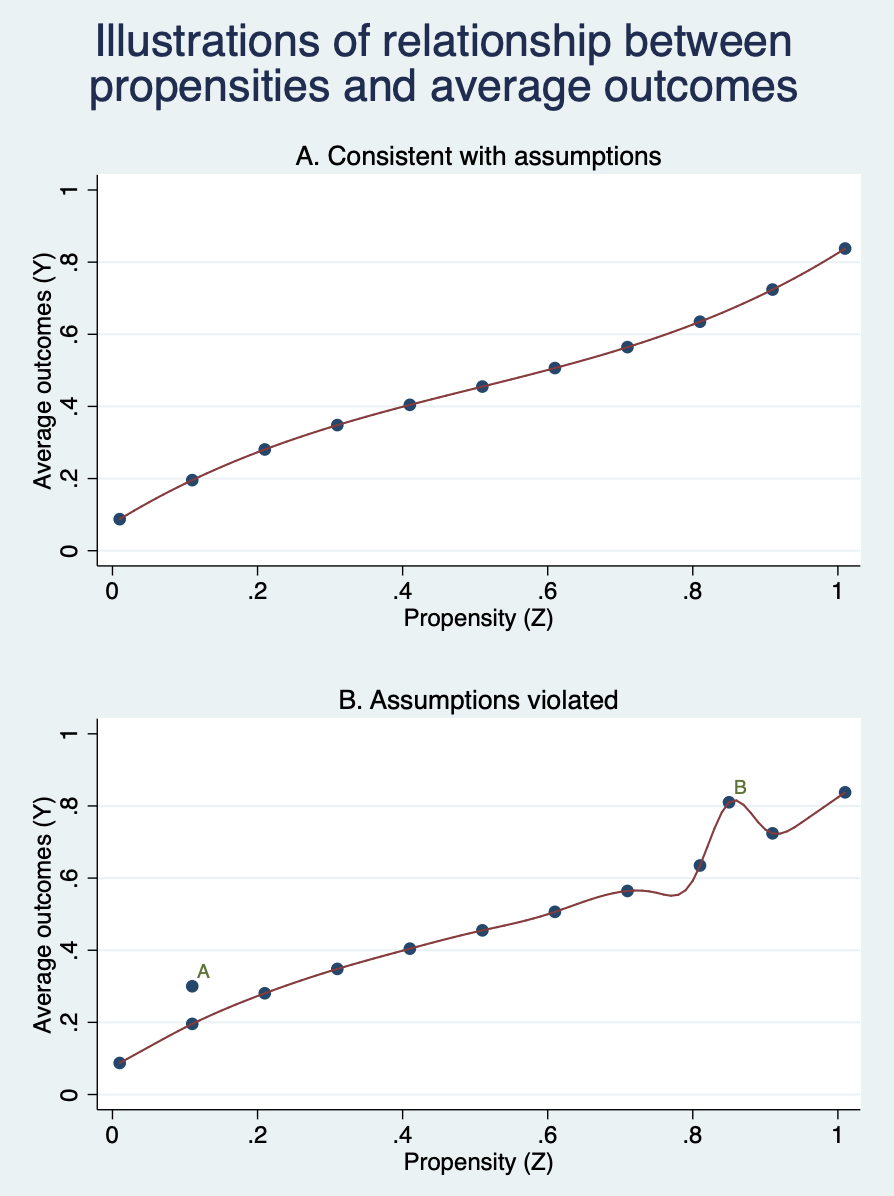
\includegraphics[width=0.8\linewidth]{jfe}
		\caption{排他性和单调性检验}
		\label{fig:jfe}
	\end{figure}
	
	\href{https://www.nber.org/system/files/working_papers/w25528/w25528.pdf}{Frandsen et al.(2019, NBER w25528)}也给出了Stata命令包testjfe。下面我们来看看stata命令:
	
	\begin{lstlisting}
		* 找到testjfe命令包
		
		findit testjfe
		
		* 加载例子的数据
		
		use http://fmwww.bc.edu/repec/bocode/f/fake_data_for_testjfe.dta,clear
		
		* 命令
		
		testjfe y d _Ijudge*,covariates(x1-x3) generate(eyj pj fit) graph
		
	\end{lstlisting}
	
	下面,我们以Stenvenson(2018)的研究为例来看看“法官固定效应”设计的IV应用。数据和代码来源于Scott Cunningham(2021):“Causal Inference:The Mixtape”的第七章。作者关注于美国费城——保释法官随机分配,且法官对于可负担水平下判决保释的倾向是不同的,更加严厉的法官设定更高的保释金,因此,更多的犯罪嫌疑人不能支付保释金,那么,这些嫌疑人就会持续被拘留。作者发现,随机拘留的增加会导致有罪判决可能性增加13\%。她认为这是由于犯罪分子认罪的增加所导致的。拘留也导致了监禁期限增加了42\%,非保释金费用提高41\%。
	
	Stenvenson(2018)的数据包含331971个观测样本,8个随机分配的保释法官。她用JIVE估计量。虽然大部分经验研究军用IV估计量,但是当存在弱工具变量和使用多个工具变量时,IV估计量会出现有限样本问题。Angrist, Imbens, and Krueger (1999)提出JIVE估计量来减轻2SLS的有限样本偏误。需要注意,JIVE也并不是完美估计量,但是,当使用多个工具变量,并存在弱工具问题时,JIVE有很多优势。
	
	\begin{lstlisting}
		use https://github.com/scunning1975/mixtape/raw/master/judge_fe.dta, clear
		
		global judge_pre judge_pre_1 judge_pre_2 judge_pre_3 judge_pre_4     \\\    
		judge_pre_5  judge_pre_6 judge_pre_7  judge_pre_8
		
		global demo black age male white 
		
		global off      fel mis sum F1 F2 F3 F M1 M2 M3 M 
		
		global prior priorCases priorWI5 prior_felChar  prior_guilt onePrior threePriors
		
		global control2     day day2 day3  bailDate t1 t2 t3 t4 t5 t6
		
		
		* Naive OLS
		* minimum controls
		
		reg guilt jail3 $control2, robust
		
		* maximum controls
		
		reg guilt jail3 possess robbery DUI1st drugSell aggAss $demo $prior $off  $control2 , robust
		
		
		* First stage
		
		reg jail3 $judge_pre $control2, robust
		
		reg jail3 possess robbery DUI1st drugSell aggAss $demo $prior $off  $control2  \\\
		 $judge_pre, robust
		
		
		
		** Instrumental variables estimation
		* 2sls main results
		* minimum controls
		
		ivregress 2sls guilt (jail3= $judge_pre) $control2, robust first
		* maximum controls
		
		ivregress 2sls guilt (jail3= $judge_pre) possess robbery DUI1st drugSell  \\\ aggAss $demo $prior $off $control2 , robust first
		
		* JIVE main results
		* minimum controls
		
		jive guilt (jail3= $judge_pre) $control2, robust
		
		* maximum controls
		
		jive guilt (jail3= $judge_pre) possess robbery DUI1st drugSell aggAss $demo \\\ 
		$prior $off $control2 , robust
		
	\end{lstlisting}
	
	表7.3给出了估计结果。用OLS时,在控制时间,拘留对认罪没有显著影响;控制罪犯特征后,拘留会提高3\%的认罪概率。当我们使用一个二值性法官固定效应最为IV时,这个效应就变得非常大(0.15-0.21),而且在5\%水平下显著。而且我们发现用JIVE估计量,效应更大。
	
	
		\begin{table}[htbp]\centering
		\scriptsize
		\caption{拘留对认罪的OLS和IV估计}
		\label{2sls_3}
		\begin{center}
			\begin{threeparttable}
				\begin{tabular}{lcccccc}
					\toprule
					\multicolumn{1}{l}{模型}&
					\multicolumn{2}{c}{\textbf{OLS}} &\multicolumn{2}{c}{\textbf{2SLS}}&\multicolumn{2}{c}{\textbf{JIVE}}\\
					\midrule
					拘留                &       -0.001&       0.029***&0.151**&0.186***&0.162**&0.212*** \\
					&   (0.002)    &     (0.002)  &(0.065)&(0.064)&(0.070)&(0.076) \\
					N& 331,971&331,971&	331,971	&331,971&	331,971	&331,971   \\
					平均认罪&0.49&	0.49	&0.49&	0.49&	0.49&	0.49
					\\
					
					\bottomrule
				\end{tabular}
				\begin{tablenotes}
					\tiny
					\item 括号里为标准误, * p$<$0.10, ** p$<$0.05, *** p$<$0.01。First model includes controls for time; second model controls for characteristics of the defendant. Outcome is guilty plea. Heteroskedastic robust standard errors in parenthesis. 
				\end{tablenotes}
			\end{threeparttable}
		\end{center}
	\end{table}
	
	注意:在使用JFE设计时,我们一定要仔细考察独立性假设、排他性约束与单调性假设。关于JFE更多的研究回顾和实践指导,可以参见\href{https://blogs.worldbank.org/impactevaluations/judge-leniency-iv-designs-now-not-just-crime-studies}{Mckenzie(2019):“Judge leniency IV designs: Now not just for Crime Studies”}。
	
	
	
	\subsection{Bartik Shift-Share IV}
	
	Bartik工具变量,也就是大家熟知的“shift-share”工具变量,得名于Bartik(1991)对区域劳动力市场的研究。但是,Goldsmith-Pinkham et al.(2020,AER)指出,最早使用该思想的研究是Perioff(1957)——产业份额可以用于预测收入水平。而且Freeman(1980)也用产业结构的变化作为劳动需求的工具变量。
	
	Bartik工具变量的核心思想是:用国家层面对不同行业产品需求的变动来测度区域劳动需求的变动。Goldsmith-Pinkham et al.(2020)认为,只要用内生变量的内积结构来构造工具变量,都可以称为Bartik IV。假设,我们想要估计下列回归方程:
	
	\begin{equation}
		Y_{l,t} = \alpha + \delta I_{l,t} +\rho X_{l,t} + \epsilon_{l,t}
	\end{equation}
	
	其中,$Y_{l,t}$表示地区l,t期的原居民工资对数,$I_{l,t}$表示t期流入地区l的移民,$X_{l,t}$是控制变量,包括地区和时间固定效应。$\delta$就是我们感兴趣的移民对原居民工资的平均处理效应。问题是,我们几乎可以肯定,移民与扰动项高度相关(Sharpe,2019)。
	
	Bartik工具变量就是l地区的初始移民份额与国家层面的移民增长率进行交乘。一个地区移民增长偏离国家平均增长可以被移民增长预测变量偏离国家层面平均增长所解释。而增长预测变量偏离国家层面的平均增长则是由于份额(shares)变动,因为在某一时期,国家层面的平均增长效应对于所有地区都是一样的。我们可以将Bartik工具变量定义为:
	
	\begin{equation}
		B_{l,t} = \sum_{k=1}^{K} z_{l,k,t^0} m_{k,t}
	\end{equation}
	
	其中,$z_{l,k,t^0}$表示来l地区自于k地区的初始$t^0$移民份额,$m_{k,t}$表示整个国家层面来自于k地的移民变动。第一项是份额(share)变量,第二项是转换(shift)变量。进入l地区的移民预测B就是每个地区流入整个国家的移民的加权平均,权重依赖于初始的移民分布。只要,我们构造了Bartik工具,我们就可以利用2SLS来估计回归——第一阶段用Bartik IV对$I_{l,t}$进行回归,然后,用预测移民$\hat{I}_{l,t}$对$Y_{l,t}$进行回归来识别出移民度原居民工资的影响。
	
	我们在进行IV研究时,通常要花费大量的时间精力和内容来阐述工具的排他性约束。但是,对于Bartik工具来说,论述排他性约束似乎更加的困难,这正是因为涉及到share项和shift项。目前,现有研究也有两个不同的视角——share视角和shift视角——来阐述Bartik工具的识别假设。
	
	\textbf{Goldsmith-Pinkham et al.(2020,AER)解释了shares视角} 。他们显示,当shifts影响第一阶段的强度时,实际上,初始shares就提供了外生变动。那么,在实践中,我们就要花费更多的时间和内容来argue为什么初始shares是外生的。
	
	尽管我们永远也无法证实排他性约束是否成立,但是,至少我们可以仔细考察一下外生性的可信度:
	
	\begin{itemize}
		\item 我们可以考察一下解释关键变动的初始份额在初始年份与其他的干扰因素的相关程度。例如,在一个贸易研究中,我们可以看看初始时期有许多计算机制造业的地区是否也有跟更多的教育。
		\item 由于存在许多加权工具变量,我们就可以进行过度识别检验——待检验的原假设“恒定的处理效应”,拒绝原假设意味着有一些工具是内生的。
	\end{itemize}
	
	Goldsmith-Pinkham et al.(2020,AER)开发了一个Rotemberg权重的\href{https://github.com/paulgp/bartik-weight}{Stata命令包和数据}来让我们可以练习一下。
	
	Goldsmith-Pinkham et al.(2020)指出,他们的研究中有两个关键的假设:位置是独立的(没有空间溢出);数据是由一系列稳态构成的。但是,Jaeger et al.(2018)对第二个假设进行了评论。我们再次考察一下移民对原居民收入的影响:
	
		\begin{equation}
		Y_{l,t} = \alpha + \delta I_{l,t} +\rho X_{l,t} + \epsilon_{l,t}
	\end{equation}

    通常,我们都会关心当期因素(例如,本地需求冲击)——影响本地居民工资和移民的因素。Bartik工具变量对于本地需求冲击是外生的。然而,jaeger et al.(2018)指出,如果面对冲击时,市场需要时间调整,那么,误差项$\epsilon_{l,t}$就会包含过去移民供给冲击的一般均衡调整效应。此时,Bartik工具变量估计量就会混合短期响应(新移民导致的工资下降)和长期响应(市场调整时间内的正向移民效应)。\textbf{我们可以在回归中增加移民的滞后项来控制这些动态效应,然后,在跑Bartik工具变量回归}:
    
    	\begin{equation}
    	Y_{l,t} = \alpha + \delta I_{l,t} + \delta_1 I_{l,t-1} +\rho X_{l,t} + \epsilon_{l,t}
    \end{equation}
	
	此时,有两个Bartik工具变量:
	
		\begin{equation}
		B_{l,t} = \sum_{k=1}^{K} z_{l,k,t^0} m_{k,t}
	\end{equation}

	\begin{equation}
	B_{l,t-1} = \sum_{k=1}^{K} z_{l,k,t^0} m_{k,t-1}
\end{equation}
	
	其中,$\delta$刻画了短期效应,$\delta_1$刻画了过去供给冲击的长期响应。
	
	总之,我们也要考察“调整动态”。
	
	
	\textbf{第二个视角就是shifts},这是由Borusyak, Hull, and Jaravel (2021,RES)提出的一个识别框架,并允许shares是内生的,例如,Goldsmith-Pinkham et al.(2020,AER)基于外生的shares。可以从冲击中来进行识别,因为share-shift IV回归系数可以从一个冲击水平的IV估计中获得。BHJ显示许多行业的外生独立冲击可以用来作为Bartik工具来识别因果效应,只要冲击与shares偏误无关即可。
	
	BHJ提供了一个简单的Share-shift IV分类。在一些情形下,使用GPSS的外生shares识别更加合适,但是还要一些情形使用shift识别方法更合适。那么,我们就需要对哪种视角的识别更合适于我们的研究进行更多的先验argue。
	
	Borusyak, Hull, and Jaravel (2021,RES)也开发了一套Bartik
	工具变量回归的Stata命令包\href{https://ideas.repec.org/c/boc/bocode/s458526.html}{SSAGGREGATE}。
	
	\begin{lstlisting}
		* 安装SSAGGREGATE
		
		ssc install ssaggregate, replace
		
		* 查看帮助文件
		
		help ssaggregate
		
	\end{lstlisting}

这个命令可以帮助我们实施shift-share (或者 "Bartik") 研究设计,in which the instrument averages a set of shocks with unit-specific weights measuring shock exposure. For example, a regional instrument is constructed from some industry shocks averaged using local employment shares, as in Bartik (1991) and Autor, Dorn, and Hanson (2013).

Based on Borusyak, Hull, and Jaravel (2021,RES), the command exploits an equivalence result. In the example of regions and locations, the regional shift-share IV coefficient can be identically obtained from a different IV regression estimated in the sample of industries. In this regression the outcome and treatment are first averaged with exposure weights to obtain industry-level aggregates; industry shocks then instrument for aggregate treatment. ssaggregate produces those industry-level aggregates.

The equivalent industry-level representation is useful when identification relies on as-good-as-random assignment of industry shocks (even if local shares are endogenous)---a quasi-experimental framework that may be plausible in many applications where the number of industries is large. The industry-level regression then helps visualize the identifying variation, produce corrected standard errors, test identifying assumptions, optimally combine multiple industry-level shocks, and more (see Borusyak, Hull, and Jaravel 2021).

	
需要增加的内容:What’s missing for an applied reader is more discussion and a framework on how to critique an IV – for example, he goes through the classic use of quarter of birth as an instrument for years of schooling when looking at impacts of schooling on earnings, where this would be an occasion to think talk through concerns of different types of parents being more likely to have kids at different types of the year. There is no discussion of overidentification tests and how they should be interpreted, nor of sensitivity analysis approaches that allow for some potential violations of the exclusion restriction.
	
	
	

	
%	\chapter{事件研究」
	
	
	
	
	\chapter{双重差分(DID)}
	
	在自然实验中,个体接受处理与否似乎是随机分配的,但是我们并不能控制这种随机性,即使我们控制了那些影响随机性的变量W,处理组和控制组之间的某些效应仍然不能估计出来。
	
	有一种方法可以消除上述问题:我们不去比较处理组和控制组之间产出水平Y的差异,而是去比较两组产出Y变化的差异,和处理前后Y变化的差异。这个估计量是处理组和控制组之间效应变化的差异,或者时间上的差异,因此,这就是我们熟知的\textbf{双重差分(DID)估计量}。这种方法似乎与事件研究设计类似。与事件研究设计不同的是,DID引入了永远不被处理的组群,也就是说,在数据中,我们既有处理组,也有未处理组。这似乎有点反直觉:未处理组可能与处理组存在差异。那么,我们不是引入了组群差异等额外的因素来影响识别结果吗?这样不是让事情变得更坏了吗?尽管可能会有这些问题,但是,DID的关键在于,我们现在有了未处理组,虽然增加了其它因素,我们就可以控制这些因素。
	
	\section{DID}
	\subsection{估计}
	
	下面,我们来看看上海对外经贸大学的司继春博士在“知乎”上举的一个例子:(\url{https://www.zhihu.com/question/24322044})
	
	现在要修一条铁路,铁路是条线,所以必然会有穿过的城市和没有被穿过的城市。记$D_i=1$,如果铁路穿过城市i;$D_i=0$,如果城市i没有被穿过。现在我们感兴趣的问题是:铁路修好以后,被铁路穿过的城市是不是经济增长更快了?我们该怎么做呢?一开始的想法是,我们把$D_i=1$的城市的GDP加总,减去$D_i=0$的城市的GDP加总,然后两者一减,即$E(Y_i\big|D_i=1)-E(Y_i\big|D_i=0)$,这样我们就算出了两类城市GDP的平均之差。如果大家还记得,这就是我们前面所讲的理想实验中的差分估计量。
	
	那么,这样做是不是就得到了我们感兴趣的铁路效应呢?不用说这样肯定有问题。如果没有问题,那我们讲完第一节就可以打铃下课,我收工回家了。我们想想,万一被铁路穿过的城市在建铁路之前GDP就高呢?为了解决这个问题,我们需要观察到至少两期,第一期是建铁路之前,第二期是建铁路之后。我们先把两类城市的GDP做铁路修建前后两期之差,即:
	
	\begin{equation}
		\Delta{Y}_i=\frac{1}{N}\sum{(Y_{i,after}-Y_{i,before})}
	\end{equation}
	
	(4)式就是第一次差分。它计算的实际是城市i建铁路前后平均GDP的增长(如果是GDP取对数,就是增长率)。接下来,我们再来计算GDP变化的平均处理效应,也就是
	\begin{equation}
		ATE=E(\Delta{Y}_i\big|D_i=1)-E(\Delta{Y}_i\big|D_i=0)
	\end{equation}
	
	这是第二次差分。这一步就把两类城市在修建铁路之前和之后的GDP增长的差异给算出来了,这就是我们要的处理效应,即修建铁路之后对城市经济的促进作用。
	
	还可以将DID估计量换一个写法。记T=1,如果时间为建铁路之后;T=0,如果时间为建铁路之前。然后,结合上面城市修建铁路与否的虚拟变量,我们可以得到下面的表3:
	
	\begin{center}
		\begin{table}[!h]
			\caption{DID估计量}\label{tab:digit}
			\begin{center}
				\begin{tabular}{|c|c|c|}
					\hline
					Treated&D=1&D=0\\
					\hline
					T=1&1&0\\
					\hline
					T=0&0&0\\
					\hline
				\end{tabular}
			\end{center}
		\end{table}
	\end{center}
	
	Treated表示在某一时期,某城市是否修建了铁路。从表3可以看出,在T=0时期,没有城市修建铁路,而在T=1期,也只有D=1的城市修建了铁路。因此,$Treated=D_i\times{T}$。我们可以写出下列回归方程:
	\begin{equation}
		Y_{it}=\alpha{D}_i+\beta{T}+\gamma{D_i\times{T}}+u_{it}
	\end{equation}
	
	其中,$Y_{it}$表示城市i在第t期的GDP。我们感兴趣的是系数$\gamma$。
	
	首先,我们将(5)式在时间维度上做一次差分:
	\begin{equation}
		\Delta{Y}_i=\beta+\gamma{D}_i+\Delta{u}_i
	\end{equation}
	
	然后,再对(6)式在个体层面做一次差分,并取期望:
	\begin{equation}
		E(\Delta{Y}_1-\Delta{Y}_0)=\gamma
	\end{equation}
	
	到此,我们得到了建铁路的经济增长效应DID估计量$\tilde{\gamma}$。
	
	这是怎么发生的呢?
	
	\begin{itemize}
		\item [1] 分离出有高铁和没有高铁这两类城市的组内变动。因为我们分离出了城市变动,我们就可以通过\textbf{城市组}来控制其的差异,进而关闭城市因素的影响——第一次差分;
		\item [2] 比较有高铁的城市的差异与没有高铁城市的差异。因为没有高铁城市的变动会受到时间的影响,那么,前面的差异比较就可以控制时间变动,进而通过\textbf{时间}来关闭那些由于时间变动产生的影响——第二次差分。
	\end{itemize}

    总而言之,我们想要的$\text{估计量} = (\text{处理后的处理组 - 处理前的处理组}) - (\text{处理后的未处理组 - 处理前的未处理组})$。这隐含意味着,未处理组的变动代表着没有发生处理时,处理组的预期变动。因此,未处理组对于DID非常关键,没有未处理组,就不能做DID。
    
    下面,我们用模拟数据来看看DiD策略的估计量。
    
    我们首先来看看我的家乡——武汉的高等教育。大家可能有所耳闻,英雄的城市武汉是中国的高等教育重镇,坐拥众多全球知名、全国一流的高等学府,其中全国最美的大学——武汉大学就在珞珈山下,东湖畔,在武大学习可以漫步在樱花大道,欣赏东湖和磨山的风景,聆听古编钟奏响的乐曲,经过张之洞、周恩来、张培刚等伟人和学术巨擎们的生活旧址与铜像前,时刻会想起那声振聋发聩地宣言”为中华之崛起而读书“!
    
    21世纪之初,武汉很多高校由于扩招而在武汉郊区假设新校区。假设2004年,武汉大学在江夏区建设了新校区,我们想看看高校新区的经济(旅游)效应如何。这个时候,我们就选择一个与江夏区比较类似的武汉郊区,例如,我的故乡黄陂区(花木兰的故乡)——没有建设高校新区——来进行对照。这个时候就形成了经典的2×2DID:两个时期——建设新校区前(2003年)和后(2004年)、两个组群——江夏区和黄陂区。
    
    % TODO: \usepackage{graphicx} required
    \begin{figure}[tbph]
    	\centering
    	\includegraphics[width=0.8\linewidth]{image/wuhan}
    	\caption{武汉赏花图。注:图片来源于网络,如侵权请联系删除}
    	\label{fig:wuhan}
    \end{figure}
    
    我们定义两个虚拟变量,是否建设新校区NU(=1,是;=0,否),建设时间前后Period(=1,后;=0,前),这个时候,我们就可以写出经典的双向固定效应(TWFE)模型:
    
    \begin{equation}
    	y_{i t}=\beta_{0}+\beta_{1} P e r i o d_{t}+\beta_{2} N U_{i}+\beta_{4} N U_{i} \times P e r i o d_{t}+\epsilon_{i t}
    \end{equation}
    
    其中,y表示结果变量——经济发展,β表示回归系数。
    
    首先,我们用stata生产一套$2\times 2$DID的数据集。也就是数据结构为两期、两个组群的面板数据。
    
    \begin{lstlisting}
    	clear      // 清除stata已存在的数据
    	local units = 2
    	local start = 1
    	local end   = 2
    	
    	local time = `end' - `start' + 1
    	local obsv = `units' * `time'
    	set obs `obsv'
    	
    	egen NU     = seq(), b(`time')  
    	egen Period      = seq(), f(`start') t(`end')   
    	
    	sort NU Period
    	xtset NU Period    // 声明面板数据类型
    	
    	lab var NU "Panel variable"
    	lab var Period  "Time  variable"
    \end{lstlisting}
	
	第二步,定义处理变量T和结果变量y:
	
	\begin{lstlisting}
		* 创建处理变量T和结果变量y
		gen T = NU==2 & Period==2    //双等号表示恒等于,即处理发生在第二个id,第二期,这时T=1,其它所有情况T=0
		
		gen btrue = cond(T==1, 3, 0)        //cond表示当T==1为真时,btru这个变量才赋值为3,否则赋值为0
		
		gen Y = NU + 3*Period + btrue*T    //利用这个函数来生成结果变量y的数据
	\end{lstlisting}

    从y的数据生成函数中,我们可以很容易的看出,在建新校区后,也就是2004年黄陂区和江夏区的结果Y的差异为4。下面,我们用图形来看看这个数据:
	
	\begin{lstlisting}
	lab de prepost1 1 "前" 2 "后"
	lab val Period prepost1
	
	twoway ///
	(connected Y Period if NU==1) ///
	(connected Y Period if NU==2) ///
	,  ///
	legend(order(1 "NU=黄陂区" 2 "NU=江夏区")) ///
	xlabel(1 2, valuelabel) ylabel(4(1)11)
	
	\end{lstlisting}
	
	% TODO: \usepackage{graphicx} required
	\begin{figure}[tbph]
		\centering
		\includegraphics[width=0.8\linewidth]{image/22dd}
		\caption{2*2DID}
		\label{fig:22dd}
	\end{figure}

从图8.2我们可以看到,蓝色的线条(黄陂区)和红色的线条(江夏区)在新建校区后的差异为4,而在新校区建设前的差异为1。因此,建设新校区前后的净变化量应该为4-1=3,即新建校区对当地经济的影响效应为3。

下面,我们可以用面板数据回归来看看结果:

	\begin{lstlisting}
	* 面板数据回归
	
	xtreg Y T Period,fe
	
\end{lstlisting}

也可以使用另一种双向固定效应命令:

\begin{lstlisting}
	
	* 常用的双向固定效应命令reghdfe
	* 如果没有安装这个程序包,请先安装:
	* ssc install reghdfe,replace
	
	reghdfe Y T, absorb(NU Period)
	
\end{lstlisting}

\subsection{推断}

大多数现实的DID应用都是多期数据,即不仅仅是两期-两组,而是多期-两(多)组,因此,我们感兴趣的变量,例如,经济增长不仅仅在江夏区和黄陂区这两个组群层面发生变化,而且也存在序列相关。Bertrand, Duflo, and Mullainathan (2004) 就指出传统标准误通常会严重低估估计量的标准偏差,因此,标准误发生下偏,即“太小”,这会使得过度拒绝原假设,显著性提高。因此,这些作者提出三种解决方案:

\begin{itemize}
	\item[1] Block bootstrapping标准误。如果block是地区,then you simply sample states with replacement for bootstrapping. Block bootstrap is straightforward and only requires a little programming involving loops and storing the estimates. The mechanics are similar to that of randomization inference。
	\item[2] 加总。加总法忽略时间维度。我们只需要对组群取平均,即平均为前后两期,然后在平均水平上跑DID。但是,如果处理时间有差异,这种方法就有一些不寻常,因为在进行余值分析前我们需要部分排除地区和时间固定效应。对于多个处理时期(后文还要详细的讲述),我们可以用结果变量对组群和时间固定效应以及协变量进行回归。然后获得处理组的余值。再然后将余值划分成前后两期,这个时候我们就忽略掉对照组。最后用余值对处理虚拟变量进行回归。需要注意的是,这个方法并没有揭示原始的点估计。
	\item[3] 聚类。学者最常用的方法就是组群聚类标准误。
\end{itemize}

还有一点需要注意:当聚类数很小时,像聚类标准误这类方法可能还不够。例如,在只有一个处理组的极端情况下,5\%的置信水平上的过度拒绝率可能高达80\%,即使用了bootstrap技术(Cameron, Gelbach, and Miller 2008; MacKinnon and Webb 2017)。在这种情况下,建议使用随机推断方法,参见Buchmueller, DiNardo, and Valletta (2011)。


	
	\section{更多经典DID的例子}
	
	
	
	\section{未处理组与平行趋势假设}
	
	既然未处理组这么重要,那么,它要具备什么特征,DID才是一个好的识别策略呢?在做DID的时候,我们需要未处理组满足一定的条件,我们称之为\textbf{平行趋势假设}。
	
	平行趋势假设说的是,如果没有发生处理,那么,处理组和未处理组仍然在处理时点后保持相同的变化趋势(与处理时点前的趋势相同)。
	
	但是,很不幸,平行趋势不可观测。它是一种反事实的情形:是假设处理没有发生的时候的情形。我们来看一个不满足平行趋势假设的例子。我们想象一下,我想看看高铁站对周围酒店餐馆的效应。例如2008年在武汉的汉口、武昌和青山都有高铁站(汉口站、武昌站和武汉站),而在武汉黄陂区则没有高铁站(黄陂区有美丽的“花木兰故乡”等旅游景点,是武汉的后花园,欢迎大家前来旅游,我可以做导游)。这个时候,我们肯定会想着用黄陂区作为未处理组。
	
	我们来看看2007年(处理前)和2008年(处理后)的武汉汉口和黄陂,用DID来识别高铁站对地区的酒店餐馆的效应。结果发现,汉口的酒店餐馆生意更差,没有黄陂的餐馆受欢迎。What弄啥呢?这一实证结果与我们的预期结果不符呀,这怎么办,收集数据做得回归都白瞎了,我的顶刊梦岁了(欲哭无泪呀)。不要着急,不要心慌,不要放弃。我们来看看是什么原因造成了这种结果。
	
	我们仔细分析一下我们的数据。突然发现,2008年,黄陂区突然新开了大量的酒店和餐馆(木兰特色的)。哦哦,原来上面的实证结果——汉口和黄陂2007/2008年的变动包括两个方面:汉口高铁站的新建和黄陂特色旅游酒店和餐馆的新建。这个时候就很明显了,我们不能得到结论,高铁站让汉口的酒店和餐馆经营变得更差了。上述DID估计并不是一个很好的估计量,即我们没有很好的识别出高铁站对酒店餐馆的效应。我们应该选择一个地区,在2008年并没有新建很多酒店和餐馆,假设武汉江夏区。但是,理想可能很丰满,现实却很骨感。我们可能根本就找不到一个在2007-2008没有发生任何变化的地区,因为那段时期的武汉到处都在大挖大建(我曾经在外省读书一年,然后过年回家,没找到回家的路,汉口站前面修建了一个二环高架,我家在火车站旁边五分钟,我硬是没找到回家的路,最后让我爸妈来接我了。)。如果我们选择武汉江夏来作为未处理组,我们可能发现,高铁站可能也没有使得汉口的酒店餐馆变得更好,因为太多的大学跑到江夏去建立新校区了,因此带过去了大量的大学生,因此,带动了江夏的“堕落街”兴起。因此,这个识别也不好。
	
	记住,DID的研究设计就是利用未处理组来代表处理组中的所有非处理变动。
	
	那么,我们可以将上述假设用下列数学表示出来:
	
	\begin{itemize}
		\item [1] 处理组在处理前后的差异 = 处理效应 + 其他因素引起的处理组变化
		\item [2] 未处理组在处理前后的差异 = 其他因素引起的未处理组变化
		\item [3] DID的效应 = 处理效应 + 其他因素引起的处理组变化 - 其他因素引起的未处理组变化
	\end{itemize}
	
	那么,对于DID来说,我们仅仅需要识别\textbf{处理效应},也就是说,“其他因素引起的处理组变化”要抵消“其他因素引起的未处理组变化”。这就是平行趋势的内容。
	
	那么,我们在做DID前,如何挑选未处理组以使得DID识别比较可信呢?我们可以做一下一些事情(并非必须,但大有益处):
	
	1、找不到理由说,未处理组在处理时点突然发生变化了;
	
	2、处理组和未处理组在许多方面都是类似的;
	
	3、处理组和未处理组的因变量在处理前有相似的变化路径。
	
	
	下面,我们用图8.3来看看。
	\begin{figure}[htbp]
		\centering
		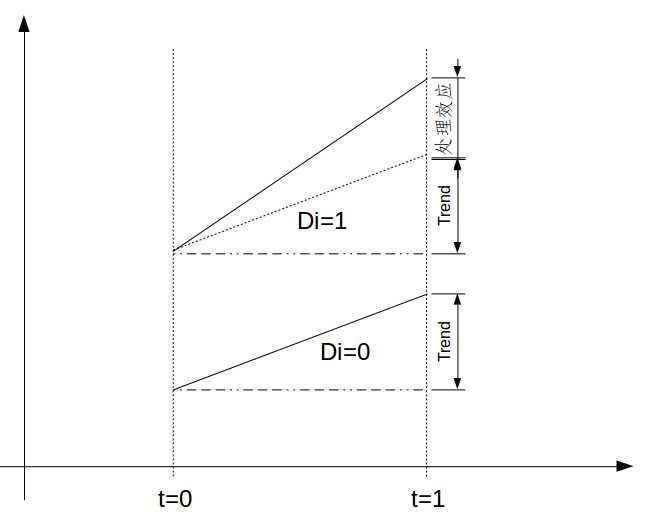
\includegraphics[width=1\textwidth]{commontrend.jpg}
		\caption{DID估计量-平行趋势}\label{fig:digit}
	\end{figure}
	
	由图8.3可以清晰地看出,DID最关键的假设是common trend,也就是两个组别在不处理的情况下,Y的趋势是一样的。那么你仍会说,铁路穿过的城市可能本身GDP也高,而GDP 高的城市按照理论GDP 增长率可能更高可能更低,所以common trend的假设可能是不对的,那怎么办?如果这个问题存在,我们可以进一步假设在控制了某些外生变量之后,common trend 是对的,比如上个问题,我们可以控制城市在t=0期的GDP level。当我们控制其他变量之后,自然不能直接减两次了,我们需要用上面说的回归式子,即对下列回归方程run OLS:
	
	\begin{equation}
		Y_{it}=\alpha{D}_i+\beta{T}+\gamma{D_i\times{T}}+X^{'}\delta+u_{it}
	\end{equation}
	
	其中,X是控制变量向量。
	
	既然common trend是DID最关键的假设,那么,我们如何评价非平行趋势呢?也就是,我们可以采取一些方法和方式来检查一下平行趋势假设,看看我们采用的DID识别是否可信。但是,需要特别提醒的是,这些方法和方式并不是检验平行趋势是否成立。即使”通过“了这些检验,我们也不能说平行趋势就一定成立。实际上,没有检验可以证实或者证伪平行趋势假设,因为它是反事实的,我们观测不到。这些检验方法更多是建议性的证据。如果没通过这些检验,那么,平行趋势假设可行度就很低。
	
	此外,下面我们来看看检验平行趋势假设在实际操作中最常用的两种方法(依情况,必做):
	
	\textbf{方法一:画时间趋势图}
	
	如果在政策干预前有多期数据,则可分别画处理组与控制组的时间趋势图(类似于上图),并直观判断这两组的时间趋势是否平行(比如,考察是否存在Ashenfelter's dip)。如果二者大致平行,则可增强对平行趋势假定的信心。然而,即使在政策干预前两组的时间趋势相同,也无法保证二者在干预后的时间趋势也相同(后者本质上不可观测,因为时间效应已与处理效应混合在一起)。另外,如果只有两期数据,则无法使用此法。
	
	\textbf{方法二:事件研究图}
		
	
	\textbf{方法三、安慰剂检验}
	
	在DID的安慰剂检验中,例如,2008年武汉修建了高铁站,那么,我们仅仅只用2008年以前的数据样本,忽略掉所有的2008年(处理后)的数据。然后,用2008年前的数据样本,我们挑选一些不同的时期,假设高铁站修建在这些时间。再然后,我们用假设的处理时点来估计DID。如果我们仍然发现了在假设的高铁站修建时点有显著的DID效应,那么,这就意味着可能还有一些其它的因素干扰了平行趋势假设。
	
	也就是说,我们估计的DID效应显著不等于0(在实际处理并未发生时)可以给我们传递的信息是,处理组的非处理变化并没有完全抵消掉未处理组的非处理变化。那么,我们还需要更多的笔墨来解释为什么我们应该相信在实际处理时点,两者相互抵消了。
	
	陈强老师于2016-10-25在微信公众号“计量经济学及stata应用”上给出更多的可操作方法:
	
	\textbf{方法四、加入更多的控制变量}
	
	从上文的讨论可知,非平行趋势可能由于遗漏变量所导致,故在回归方程中加入更多控制变量,或可缓解内生性。但此法在实践中不易实施。
	
	\textbf{方法五、假设线性时间趋势}
	
	如果假设时间趋势为线性函数,则可加入每位个体的时间趋势项:
	
	在具体回归时,加入个体虚拟变量与时间趋势项 t = 1, 2, ... , T 的交互项即可。然而,线性时间趋势毕竟是较强的假定,不一定能成立。故此法也不完全解决问题,但可作为稳健性检验。
	
	\textbf{方法六、三重差分法}
	
	在一定条件下,可通过引入两个控制组,进行三次差分,称为“三重差分法”(difference-in-differences-in-differences,简记DDD),这样可以更好地控制时间趋势的差异,使得平行趋势假定更易成立。有关DDD的进一步介绍,参见陈强(2014,第343页)。
	
	最后但也很重要的事(经常被忽略):平行趋势意味着我们还要认真仔细地想想我们的因变量是如何测度和进行数据转换的。因为平行趋势并不仅仅是因果效应的假设,它也是处理组和未处理组在处理前的差异大小基本保持恒定,这就意味着我们还要考虑我们如何测度这个差异的问题。我们以对数转换为例,如果因变量$Y$的平行趋势成立,那么,$ln(Y)$就不成立,反之亦然。
	
	这是一件显而易见的事,但是我们当中许多人从来不会去考虑这个问题。因此,我们仔细思考一下因变量满足平行趋势的形式是什么,然后我们就使用这种形式的因变量。
	
	\section{DID在Stata中的实现}
	
	要估计自然实验中的平均处理效应,如果直接在stata中run(9)式,那么,直接使用普通的面板数据命令$xtreg$即可。而DID则有专门的命令估计。厦门大学赵西亮老师的书里介绍了一种DID的命令,$diff$,其语法和基本选项为:
	\begin{lstlisting}
		diff outcome var [if] [in] [weight], period(varname)
		\underline{t}reated(varname)~[\underline{c}ov(varlist)
		\underline{k}ernel~id(varname)~bw(\#)~\underline{kt}ype(kernel)~rcs~\\
		\underline{qd}id(quantile)~\underline{ps}core(varname)~\underline{lo}git~\\
		\underline{su}pport~\underline{add}cov(varlist)~\underline{c}luster(varname)\\
		~robust~bs~\underline{r}eps(int)~test \underline{rep}ort~\underline{nos}tar~export(filename)]
	\end{lstlisting}
	
	outcome-var是结果变量,$\underline{p}eriod(varname)$告诉软件时期变量,\underline{t}reated(varname)告诉软件处理变量。其他命令(也就是中括号里的命令)都是可选择的。参见赵西亮(2017)第177页。
	
	\textbf{操作实例:}
	下面,我们利用Card and Krueger(1994,AER)的数据为例,估计新泽西州最低工资调整对新泽西州快餐业就业的影响,数据为两期面板数据,主要变量有:id为快餐;t为时间,最低工资调整前为0,调整后为1;treated为分组变量,1为新泽西,0为宾夕法尼亚;fte为全职就业人数,协变量有bk、kfc、roys、wendys。如下图2所示:
	\begin{figure}[htbp!]
		\centering
		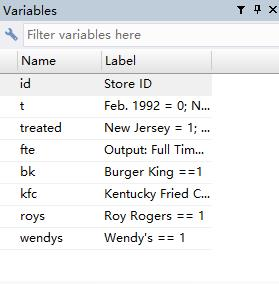
\includegraphics[width=1\textwidth]{var.jpg}
		\caption{变量}\label{fig:digit}
	\end{figure}
	
	首先,安装DID命令:$ssc~install~diff,~replace$
	
	然后,我们就可以在stata中输入DID命令估计回归系数。
	
	不控制任何协变量时的结果:
	
	diff~fte,~period(t)~treated(treated)~robust
	\begin{figure}[htbp!]
		\centering
		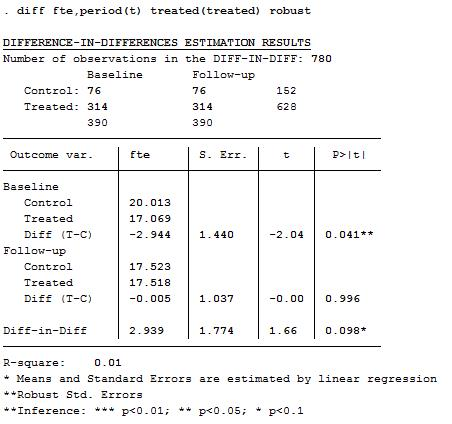
\includegraphics[width=0.4\textwidth]{DIDresults.jpg}
		\caption{DID结果}\label{fig:digit}
	\end{figure}
	
	控制协变量时的结果:
	
	diff~fte,~period(t)~treated(treated)~robust~cov(bk kfc roys)
	\begin{figure}[htbp!]
		\centering
		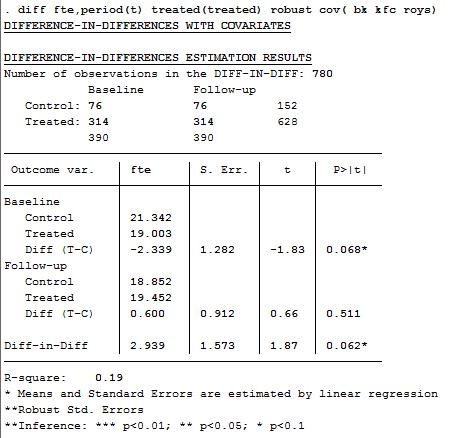
\includegraphics[width=0.4\textwidth]{DIDcov.jpg}
		\caption{控制协变量的DID结果}\label{fig:digit}
	\end{figure}
	
	
	\section{动态处理效应}
	
	在上文中,我们所讨论的DID都是两组和两期($2 \times 2$),尤其是两期——处理前和处理后。但我们在现实中遇到的情形肯定不止两期,那么,DID设计可以使用吗?答案是当然,但是附带条件。(8.9)式的双向固定效应(TWFE)模型可以用于多期处理的情形:将多期划分为两个大类——前和后,然后估计单一效应——整个处理后时期的效应。
	
	但是这样以来,我们也忽略了很多有趣的事。例如,处理效应会随着时间的推移慢慢发生变化吗?变大还是变小?处理后的时期有多长,一天,一月,一年,还是5年?肯定有人为会说,好吧,那我们为什么不把每一期的效应都估计出来呢?这个可行吗?
	
	当然可行!
	
	我们仅仅只需要将上述DID模型进行一点点修正就可以得到每个时期的效应。换言之,我们可以估计\textbf{动态处理效应}。此时,我们可以将处理前一期设置为$t=0$,处理前的倒数第二期设置为$t=-1$,实施处理的时期为$t=1$,处理后的第二期设置为$t=2$,以此类推。然后,将处理变量与每一期的时间虚拟变量进行交互,动态处理效应的DID模型就修正完毕!模型设定如下:
	
	\begin{equation}
		Y_{i,t} = \alpha_i + \gamma_t + \sum_{m = -G}^{M} \beta_m D_{i,t-m} + \phi X_{i,t} + C_{i,t} + \epsilon_{i,t}
	\end{equation}
	
	其中,$\alpha_i$表示个体固定效应,$\gamma_t$表示时间固定效应,$X_{i,t}$表示控制变量,$C_{i,t}$表示潜在不可观测的、与处理(政策)相关的混淆变量。$ \sum_{m = -G}^{M} \beta_m D_{i,t-m} $ 意味着处理有动态效应。t期的结果最多受到t之前的$M \le 0 $期处理变量的影响,也最多受到t之后的$G \le 0$期的影响。而系数$\{\beta_m\}_{m=-G}^{M}$就表示这些动态效应的程度。通常,G和M的值是由我们自己确定的。
	
	(8.10)式为我们提供了许多信息:
	
	1、处理前的系数$\beta_{-M},...,\beta_{-2},\beta_{-1}$应该接近于0,或者置信水平不显著。也就是说,处理前应该不存在处理效应。这可以看做是一种安慰剂检验的形式——处理前,DID回归会发现处理效应吗?希望各位不会得到显著的处理效应!
	
	% TODO: \usepackage{graphicx} required
	\begin{figure}[tbph]
		\centering
		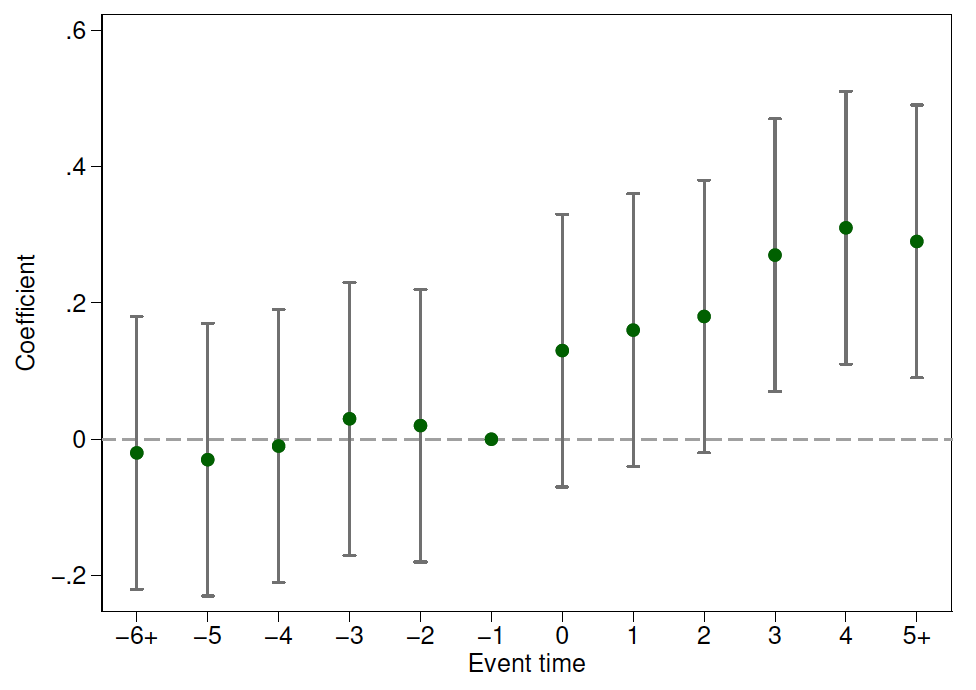
\includegraphics[width=0.7\linewidth]{dynamicDID}
		\caption{动态处理效应图,来源于Freyaldenhoven et al.(2021)。}
		\label{fig:dynamicdid}
	\end{figure}
	
	如图8.5所示,圆点表示估计系数,上下限表示置信区间,在处理前,DID估计系数都在0附近。
	
	
	2、处理后的系数$\beta_{1},\beta_{2},...,\beta_{G}$在处理后每一期的DID估计效应。
	
	在Stata中,我们仅仅只需要增加相应的交互项,$i.time \#\# i.treat$。
	
	当我们做出了动态处理效应后,我们就可以将结果展示出来了。
	
	此时的你还在为展示结果而发愁吗?你还在为自己的动态处理效应结果表格太多太长而苦恼吗?你还在为结果的清晰易懂而掉头发吗?你还在为没有充分展示自己刻苦跑回归而遗憾吗?
	
	好消息!好消息!Simon Freyaldenhoven, Christian Hansen, Jorge Pérez Pérez, and Jesse M. Shapiro(2021)给出了许多可视化动态处理效应的建议,让我们清晰地、尽可能多地展示这些回归结果和有用的信息。他们建议,我们可以做两个方面的工作,再来展示动态处理效应的图。第一,展示不同时期k的累积处理效应,即k期前的所有估计系数之和$\sum{m=-G}^{k}\beta_m$。为了简化估计积累效应,可以采用处理变量的变化项来修正动态处理效应DID(9.7)。第二,为了可视化过度识别信息,我们可以画出政策影响时期外的累积处理效应,这个时候,我们就需要修正模型(9.7)来包含t期的处理会导致$t-G$前的$L_G$期和$t+M$后的$L_M$期结果都会发生变化。
	
	因此,我们将(9.7)修正为:
	
		\begin{equation}
		Y_{i,t} = \alpha_i + \gamma_t + \sum_{k= -G-L_G}^{M+L_M-1} \delta_k \Delta D_{i,t-k} + \delta_{M+L_M}D_{i,t-M-L_M} + \delta_{-G-L_G-1}(-D_{i,t+G+L_G}) + \phi X_{i,t} + C_{i,t} + \epsilon_{i,t}
	\end{equation}
	
	其中,$\Delta$表示一阶差分算子。注意,(9.8)也可以应用于交叠DID的情形(下文会更详细的讲解),这个时候,$\Delta D_{i,t-k}$表示个体i在t期前的k期是否被处理,$(1-D_{i,t+G+L_G})$表示个体i在t期后的$G+L_G$期是否被处理,$D_{i,t-M-L_M}$表示个体i在t期前的至少$M+L_M$是否被处理。
	
	参数$\{\delta\}_{k=-G-L_G-1}^{k=M+L_M}$可以理解成不同时期的累积处理效应。尤其是,结合(9.7)意味着
	
\begin{equation}
\delta_k =	\begin{cases}
		 0  & \text{当} k< -G \\
		\sum_{m=-G}^{k}\beta_m    &\text{当}-G \le k \le M \\
		\sum_{m=-G}^{M}\beta_m  & \text{当} k \ge M 
	\end{cases}
\end{equation}
		
我们在展示动态处理效应图时,其核心就是画出$\{k,\dot{\delta}_k\}_{k=-G-L_G-1}^{k=M+L_M}$的散点图。Simon Freyaldenhoven, Christian Hansen, Jorge Pérez Pérez, and Jesse M. Shapiro(2021)给出了实践操作中展示处理效应图的7点建议:

\textbf{1、当估计(9.8)时,标准化$\delta_{-G-1}=0$}。

图9.6 展示了标准化$\delta_{-1}=0$的动态效应图。两张图有类似的处理前趋势。在处理时间-1后,图9.6(a)仍然显示平滑的处理前趋势,而9.6(b)则显示了“跳跃”。且图中包含了95\%的置信区间。我们标准化$\delta_{-1}=0$就可以很容易的使用置信区间来检验点假设——处理-时间趋势在时期-1和k处相同($\delta_{-1}=\delta_k$)。例如,设定k=0,读者就能很容易地从图9.6(b)中得到结论:处理时间0处的结果发生了显著地变化。而从9.6(a)可以看出,处理时点0处的结果并没有发生显著地变化。

% TODO: \usepackage{graphicx} required
\begin{figure}[tbph]
	\centering
	\includegraphics[width=1\linewidth]{sug1}
	\caption{动态效应的标准化事件-时间(建议1)\\ 图片来源于:Simon Freyaldenhoven, Christian Hansen, Jorge Pérez Pérez, and Jesse M. Shapiro(2021,NBER, w29170)}
	\label{fig:sug1}
\end{figure}


\textbf{2、在图中加入系数$\delta_{k^\star}$的标签,其值放入一个括号中,且值为}:

\begin{equation}
	\frac{\sum_{(i,t):\Delta D_{i,t+k^\star} \neq 0}Y_{i,t}}{|(i,t):\Delta D_{i,t+k^\star} \neq 0|}
\end{equation}
	
	图9.7展示了建议2的括号标签——y轴0点处。这个标签可以很容易地让读者理解估计的积累政策效应的大小。例如,图9.7(a)中系数估计量$\hat{\delta}_3$意味着第3期(相对于处理时间-1期)的政策对结果的积累效应大约为-0.73,这个效应比较适中(相对于括号标签41.94——政策变化前一期的因变量样本均值)。
	
	% TODO: \usepackage{graphicx} required
	\begin{figure}[tbph]
		\centering
		\includegraphics[width=1\linewidth]{sug2}
		\caption{系数标签(建议2)\\ 图片来源于:Simon Freyaldenhoven, Christian Hansen, Jorge Pérez Pérez, and Jesse M. Shapiro(2021,NBER, w29170)}
		\label{fig:sug2}
	\end{figure}
	
	
	\textbf{3、除了为处理时间路径的单个要素画出点置信区间外,还要为结果$\delta$的处理时间路径画一条双向sup-t置信带宽。}
	
	图9.8呈现了建议3的增加双向置信带宽,即在点置信区间外的线条。任何落入点置信区间外的处理时间路径的值都可以理解成统计上与对应估计量不一致,任何没有完全通过置信带宽的处理时间路径都可以理解成统计上与估计路径不一致。例如,在9.8的两张图中,用双向置信带宽,我们不能拒绝所有处理前的处理时间路径等于0。但用点置信区间,我们可以得到结论$\hat{\delta}_{-5}$是统计显著的。除非我们已经预先设定我们只对原假设——$\delta_{-5}=0$——感兴趣,否则,基于双向置信带宽的结论似乎更合理一些。
	
		% TODO: \usepackage{graphicx} required
	\begin{figure}[tbph]
		\centering
		\includegraphics[width=1\linewidth]{sug3}
		\caption{双向置信带宽(建议3)\\ 图片来源于:Simon Freyaldenhoven, Christian Hansen, Jorge Pérez Pérez, and Jesse M. Shapiro(2021,NBER, w29170)}
		\label{fig:sug3}
	\end{figure}
	
		\textbf{4、在图中包含下列假设的Wald检验p值:}
		
		$$
		\begin{array}{lrl}
			H_{0}: \delta_{k}=0, & -\left(G+L_{G}+1\right) & \leq k<-G (\text{no pre-trends})\\
			H_{0}: \delta_{M}=\delta_{M+k}, & 0 & <k \leq L_{M}  (\text{dynamics level off})
		\end{array}
		$$
		
		图9.9展示了增加两个p值,给定$L_G=0$和$L_M=1$两张图都没有拒绝待检验假设。建议4中的待检验假设的精确声明都有赖于$L_G$和$L_M$的选择。即它们控制着(9.7)式施加给(9.8)式过度识别约束的数量。实践中,对于$L_G$和$L_M$的选择采用经验规则(参考经典文献的选择)。
	
		% TODO: \usepackage{graphicx} required
	\begin{figure}[tbph]
		\centering
		\includegraphics[width=1\linewidth]{sug4}
		\caption{增加Wald检验p值(建议4)\\ 图片来源于:Simon Freyaldenhoven, Christian Hansen, Jorge Pérez Pérez, and Jesse M. Shapiro(2021,NBER, w29170)}
		\label{fig:sug4}
	\end{figure}

	\textbf{5、设定$L_M=1$和$L_G=M+G$}
	
	设定$L_M=1$可保证检验我们的假设:过去超过M期的政策变量变化并不会改变结果。而设定$L_G=M+G$则可以使事件图“对称”,从这个意义上来说,可以检验政策可能影响结果的期限内的处理前趋势。例如,图9.9设定了M=5,G=0。


	\textbf{6、Plot the least “wiggly” confound whose path is contained in the Wald region $CR(\delta)$ for the event-time path of the outcome. Specifically, plot  $\delta*(v*)$, where}
		
		\begin{equation}
			\begin{aligned}
				p^{*} &=\min \left\{\operatorname{dim}(v): \delta^{*}(v) \in C R(\delta)\right\} \text { and } \\
				v^{*} &=\arg \min _{v}\left\{v_{p^{*}}^{2}: \operatorname{dim}(v)=p^{*}, \delta^{*}(v) \in C R(\delta)\right\}
			\end{aligned}
		\end{equation}
	
	Figure 9.10 illustrates Suggestion 6 by adding the path $\delta*(v*)$ to the plot in Figure 9.9. In Figure 9.10(a), the estimated event-time path is consistent with a confound that follows a very “smooth” path, close to linear in event time, that begins pre-event and simply continues post-event. We suspect that in many economic settings such confound dynamics would be considered plausible, thus suggesting that a confound can plausibly explain the entire event-time path of the outcome, and therefore that the policy might plausibly have no effect on the outcome. In Figure 9.10(b), by contrast, the estimated event-time path demands a confound with a very “wiggly” path. We suspect that in many economic settings such confound dynamics would not be considered plausible, thus suggesting that a confound cannot plausibly explain the entire event-time path of the outcome, and therefore that the policy does affect the outcome.
	
	% TODO: \usepackage{graphicx} required
	\begin{figure}[tbph]
		\centering
		\includegraphics[width=1\linewidth]{sug6}
		\caption{增加Wald检验p值(建议6)\\ 图片来源于:Simon Freyaldenhoven, Christian Hansen, Jorge Pérez Pérez, and Jesse M. Shapiro(2021,NBER, w29170)}
		\label{fig:sug6}
	\end{figure}
		
			\textbf{7、如果用一个比(9.7)式更多限制的回归模型来概述效应大小,我们就应该可视化下列限制:}

            1、在预期限制下估计(9.7);
            
            2、用(9.9)式将(9.7)式估计量转换成积累效应;
            
            3、将估计的累积效应画在事件研究图上。

Figure 9.11 illustrates this suggestion in a hypothetical example in which the more restrictive model assumes that the policy effect is static, i.e., that the current value of the policy affects only the current value of the outcome. Comparison of the two event-time paths provides a visualization of the fit of the more restrictive model. The uniform confidence bands permit ready visual assessment of more restrictive models. In the case shown in Figure 9.11, the more restrictive model is not included in the uniform confidence band, implying that we can reject the hypothesis that the effect of the
policy is static. Figure 9.11 also displays the p-value from a Wald test of the more restrictive model, which also implies that the more restrictive model is rejected. The Wald test may be more powerful for testing this joint hypothesis than the test based on the sup-t bands, but its implications are harder to visualize in this setting (Olea and Plagborg-Møller 2019).



% TODO: \usepackage{graphicx} required
\begin{figure}[tbph]
	\centering
	\includegraphics[width=1\linewidth]{sug7}
	\caption{评价一个模型的拟合程度(建议7)\\ 图片来源于:Simon Freyaldenhoven, Christian Hansen, Jorge Pérez Pérez, and Jesse M. Shapiro(2021,NBER, w29170)}
	\label{fig:sug7}
\end{figure}
	
	Simon Freyaldenhoven, Christian Hansen, Jorge Pérez Pérez, and Jesse M. Shapiro(2021,NBER, w29170)开发的stata命令包——xtevent来实现上述建议。
	
	\begin{lstlisting}
		* 首先,找到xtevent命令包
		
		findit xtevent
		
		* 或者直接安装命令包
		
		ssc install xtevent, replace
		
	\end{lstlisting}
	
	
	
	\section{交叠DID}
	
	迄今为止,我们讨论的处理期都是同一时点,也就是说,对于所有的个体来说,都在同一期发生处理。但是,现实社会中,很多事件发生在不同的时点,也就是说,不同个体受到处理的时间可能不同。这个时候,我们还可以按照上面的双向固定效应(TWFE)估计量那样来理解DID估计系数吗?明确的答案:肯定不行!
	
	\subsection{异质性处理时点下TWFE模型的问题}
	
	例如,我们想研究一下武汉的大学在郊区建新校区对当地经济的影响。我们可能知道,武汉的很多大学在21世纪初(例如2003年)都在武汉江夏区建设新校区,而在2010年在武汉黄陂区建设新校区。江夏区和黄陂区都有建设大学的前后时期,但是它们的“建设”时间不同。那么,研究大学新校区对当地经济社会的影响效应有什么问题吗?
	
	从研究设计的角度来看,没有任何问题,我们只需要把每个2*2的组群-时间放在一起即可。但是,Goodman-Bacon(2020)指出,从统计的角度看,异质性处理时点会使得双向固定效应(TWFE)回归不再有效。甚至在一些情形下,本来大学新校区会促进当地经济社会发展,但是,我们用TWFE来估计DID估计量会得到负向效应。
	
	之所以会产生这样的后果,原因非常的复杂,我们在这里并不去回顾这些复杂的数学推导,如有兴趣,可以参考Baker(2019):“\href{https://andrewcbaker.netlify.app/2019/09/25/difference-in-differences-methodology/}{Difference-in-Differences Methodology}”、Callaway and Sant’Anna(2020):“\href{https://cran.r-project.org/web/packages/did/vignettes/multi-period-did.html}{Introduction to DiD with Multiple Time Periods}”。总而言之,多期异质性处理时点的TWFE会将已经处理的组群作为控制组,这就会使得处理前的平行趋势不再满足。(1)如果效应本身就具有动态性,或者处理效应在组群间变动,那么,我们设定的回归不满足平行趋势。(2)如果处理效应会随着时间而增强,那么,“处理的控制组”会具有向上变动的趋势,而“刚刚受到处理”的组群则没有这个趋势,因此,平行趋势不成立,识别失败。正如Sun and Abraham (2020)指出:不同时期的效应会彼此交叠和影响。这也是被称为“交叠DID”的原因。
	
		2018以来,关于交叠DID的双向固定效应的问题及其稳健估计量的论文呈现出了爆炸性的增长,如表9.2和9.3所示(更多关于DID的进展信息,参见\href{https://asjadnaqvi.github.io/DiD/}{Asjad Naqvi的DID主页})。这么多的论文确实把我们”炸伤“了,要跟踪这些论文,并充分学习、理解它们之间的差异,有时候真的比走蜀道还难。要知道,人们都习惯于“吃老本”,因为我们前期已经在这些老本上花了大量的时间和精力,而且对于“发论文”来说似乎也够用,因此,学习新的知识花的时间和精力成本太大,而且边际收益也是递减的。但是,做真正的研究和教学来说,学习这些最新的进展肯定是必须的,因为学生们需要老师去指引。
	
	下面,我们就带大家来学习一下交叠DID估计。我们忽略那些“艰涩难懂”的数学与统计细节,更多关注于这些最新的稳健DID估计量的直观含义与Stata操作。
	
	\begin{table}[htbp]
		\centering
		\caption{交叠DID的Stata包及对应文献}
		\begin{longtable}{|c|c|c|}
			\hline
			Stata包&安装  & 参考文献 \\
			\hline
			bacondecomp& \tabincell{c}{ ssc install bacondecomp, replace
				\\
				or
				\\
				net install ddtiming, from (https://tgoldring.com/code/)} & \tabincell{c}{ Andrew Goodman-Bacon\\(2021). Difference-in-\\differences with \\variation in \\treatment timing. \\Journal of Econometrics}\\
			\hline
			eventstudyinteract & ssc install eventstudyinteract, replace & \tabincell{c}{ Liyang Sun, Sarah \\Abraham (2020).\\ Estimating dynamic \\treatment effects\\ in event studies with\\ heterogeneous treatment \\effects. \\Journal of Econometrics}\\
			\hline
			did\_multiplegt &	ssc install did\_multiplegt, replace & \tabincell{c}{Clément de Chaisemartin,\\ Xavier D'Haultfoeuille \\(2020). Two-Way \\Fixed Effects Estimators \\with Heterogeneous \\Treatment Effects. \\American Economic \\Review.\\
				Clément de Chaisemartin, \\Xavier D'Haultfoeuille \\(2021). Two-way\\ fixed effects regressions\\ with several treatments.\\
				Clément de Chaisemartin, \\Xavier D'Haultfoeuille \\(2021). Difference-in-\\Differences Estimators \\of Inter-temporal \\Treatment Effects.} \\
			\hline
			did\_imputation&	ssc install did\_imputation, replace& \tabincell{c}{Kirill Borusyak , \\Xavier Jaravel , \\Jann Spiess  (2021). \\Revisiting Event Study \\Designs\\: Robust and Efficient \\Estimation.} \\
			\hline
			
			drdid &	ssc install drdid, replace& \tabincell{c}{ Pedro H.C. Sant'Anna ,\\ Jun Zhao (2020).\\ Doubly robust\\ difference-in-\\differences estimators, \\Journal of Econometrics.}\\
			\hline
			
			
		\end{longtable}
	\end{table}
	
	
	\begin{table}[htbp]
		\centering
		\caption{交叠DID的Stata包及对应文献(续表)}
		\begin{longtable}{|c|c|c|}
			\hline
			Stata包&安装  & 参考文献 \\
			\hline
			
			csdid &	ssc install csdid, replace& \tabincell{c}{Brantly Callaway, \\Pedro H.C. Sant'Anna  \\(2020).\\ Difference-in-\\Differences with multiple \\time periods, \\Journal of Econometrics.}\\
			\hline
			flexpaneldid &	ssc install flexpaneldid, replace&\tabincell{c}{Antje Weyh\\	Eva Dettmann, \\Alexander Giebler,\\ Antje Weyh (2020).\\ Flexpaneldid: A \\Stata Toolbox \\for Causal Analysis \\with Varying Treatment \\Time and Duration. \\IWH Discussion Papers \\No. 3/2020} \\
			\hline
			
			xtevent	& ssc install xtevent, replace&\tabincell{c}{Simon Freyaldenhoven, \\Christian Hansen, \\Jesse M. Shapiro\\ (2019). Pre-event \\Trends in the Panel \\Event-Study Design.\\ American Economic\\ Review.}\\
			\hline
			did2s&	ssc install did2s, replace	& \tabincell{c}{John Gardner (2021). \\Two-stage differences \\in differences.}\\
			\hline
			stackedev &	github install joshbleiberg/stackedev&  \tabincell{c}{Doruk Cengiz , \\Arindrajit Dube , \\Attila Lindner,\\ Ben Zipperer  (2019). \\The effect of minimum \\wages on low-wage\\ jobs. The Quarterly \\Journal of Economics.} \\
			\hline
			
			eventdd	&ssc install eventdd, replace&	 \tabincell{c}{Damian Clarke,\\ Kathya Tapia (2020). \\Implementing the Panel \\Event Study.}\\
			\hline
			staggered\_stata&	github install jonathandroth/staggered\_stata&	 \tabincell{c}{Jonathan Roth , \\Pedro H.C. Sant'Anna  \\(2021). Efficient\\ Estimation for Staggered \\Rollout Designs} \\
			\hline
			
		\end{longtable}
	\end{table}
	
	
	Goodman-Bacon(2020)指出,\textbf{TWFE估计量实际上是所有可能的$2 \times 2$DID估计量的加权平均}。其权重与组群规模和每一对$2 \times 2$处理指标的方差成一定比例——面板数据中间处理的单元有最高的权重。他还推导了,有 一些$2 \times 2$DID估计量用特定时点处理的组群作为处理组,而从未处理的组群作为控制组,另一些$2 \times 2$DID估计量则用两个不同时点处理的组群——处理开始前,后一次处理的组群作为控制组,而处理开始后,前一次处理的组群作为控制组。因此,当处理效应不随时间变化时,$2 \times 2$DID估计量就是组间处理效应(以方差为权重)加权平均,且所有权重都为正。但是,当处理效应随时间变化时,有一些$2 \times 2$DID估计量就会出现负的权重。这是因为已经处理的组群被当作了控制组,其随时间变化的处理效应的比重会发生变化,但TWFE-DID估计量忽略了这一点。
	
	下面,我们还是来思考一下武汉的大学去郊区建设新校区对当地经济社会发展产生的效应:江夏区从2003年开始建设新校区,黄陂区从2010年开始建设新校区。假设我们有1998-2019年武汉两个郊区经济社会发展数据。这个数据集允许我们比较两个不同的DID:
	
	第一,我们关注于1998-2010年,如图9.12左图所示。在这一段时期,黄陂区从未建设大学新校区,而江夏区在2003年“被处理”了,因此,我们可以将黄陂区作为对照组,将江夏区作为处理组来估计大学新校区对经济社会发展的影响。
	
	第二,我们也可以关注2003-2019年,如图9.12右图所示。这一时期,江夏新建大学校区的状态并为发生变化,而黄陂区咋2010年有了新校区。因此,可以将江夏作为对照组,黄陂区作为处理组来估计大学新校区对经济社会发展的响应。
	
	
	% TODO: \usepackage{graphicx} required
	\begin{figure}[tbph]
		\centering
		\includegraphics[width=1\linewidth]{GB_decom}
		\caption{Goodman-Bacon分解}
		\label{fig:GB_decom}
	\end{figure}
	
	Goodman-Bacon(2020)显示,所有交叠DID的TWFE估计量都可以按照图9.12的方式进行分解:(1)先处理的组群(江夏)与后处理的组群(黄陂)在处理前时期的差分;(2)先处理的组群(江夏)在处理后时期与后处理组群(黄陂)的差分;(3)不同处理时点的组群与从未处理组群(如果存在)的差分。因此,他提出用三种差分的加权平均来作为交叠DID估计量。因此,TWFE的DID估计量只有在不随时间变化的同质处理效应情形下才适用,而在交叠处理时点情形,还采用其它方法。
	
	据此,更加突出,在做DID之前一定要检验面板数据的平行趋势是否成立。当遇到交叠处理时点时,我们要修正画平行趋势图的方法——重新寻找中心处理点,并堆叠所有可能的$2 \times 2$DID。关键点在于识别同时依赖于处理前后的共同趋势。由于我们要重新加权平均这$2 \times 2$DID估计量,因此,有一些组群不满足共同趋势假设的情况比另一些组群要更严重。好吧!优陷入死胡同了?没有!Goodman-Bacon(2020)也提出了一个检验——方差加权的共同趋势——来评价所有观测到的偏离的严重程度:分解并画出$2 \times 2$DID估计量的变动。Stata命令包为\textbf{bacondecomp}:
	
	\begin{lstlisting}
		* 安装bacon分解包
		
		ssc install bacondecomp, replace
		
		* 加载Stevenson and Wolfers' (2006)关于无过错离婚改革对女性自杀效应的数据
		
		use http://pped.org/bacon_example.dta
		
		* 声明面板数据
		
		xtset stfips year
		
		* 估计双向固定效应TWFE
		
		xtreg asmrs post pcinc asmrh cases i.year, fe robust
		
		* Goodman-Bacon (2020)的DID分解应用于上述TWFE模型
		
		bacondecomp asmrs post pcinc asmrh cases, stub(Bacon_) robust
		
		* 显示详细的分解信息
		
		bacondecomp asmrs post pcinc asmrh cases, ddetail
		
		
	\end{lstlisting}
	
    下面,我们用来自于bacondecomp包的案例和数据来说明一下Goodman-Bacon(2020)的DID分解:Stevenson and Wolfers' (2006)研究了无过错离婚改革对女性自杀的影响。图9.13展示了Goodman-Bacon分解的结果。红色的水平线表示DID估计量(-3.08)——y轴值乘以x轴的权重。三角点表示一个时变的组群作为处理组,1964年改革前的组群作为对照组。叉叉点表示一个时变处理的组群作为处理组,非改革组群作为对照组。
	
	
	% TODO: \usepackage{graphicx} required
	\begin{figure}[tbph]
		\centering
		\includegraphics[width=1\linewidth]{GB_decomp_example}
		\caption{无过错离婚改革的效应:Goodman-Bacon分解}
		\label{fig:GB_decomp_example}
	\end{figure}
	
\subsection{事件研究与Bacon分解}


    Goodman-Bacon(2020)建议在异质性处理时点情形下,使用事件研究设计。下面,我们跟随Cheng and Hoekstra(2013)来看看事件研究和Bacon分解的用法。他们评估了美国枪支改革对暴力的影响。2012年2月26日,在美国佛罗里达的斯坦福,乔治.齐默尔曼开枪杀死了年仅17岁的非裔美国人本杰明.马丁。马丁从便利店回家,齐默尔曼尾随了很长一段路,并向警察报警说马丁行为很诡异,警察劝齐默尔曼离开。但齐默尔曼并未听警察的劝告,并在跟踪马丁的过程中激怒了马丁,两个人起了激烈的冲突。最终,齐默尔曼开枪杀死了马丁。齐默尔曼认为自己是正当防卫,并提出无罪辩护。陪审团也释放了他。
    
    陪审团认为齐默尔曼的行为是合法的,因为在2005年,佛罗里达改革规定了致命性正当防卫的使用情形。以前,致命性正当防卫只在家里使用才是合法的,但一部新的法律SYG将上述情形扩展到了公共区域。在2000-2010年间,美国21个州进行了类似的致命性正当防卫的范围。这些改革之后,只要人们感觉到危险,他们都可以使用致命性正当防卫来进行反击。甚至在一些州,只要人们感觉害怕就可以使用暴力回击。因此,检察官要起诉,就要证明“害怕”的感觉不合理,这几乎是不可能证明的。
    
    从经济学的视角来看,这些改革降低了开枪杀人的成本。人们能用致命性正当防卫来仅仅只是让自己害怕的感觉消失。因此,我们可以预期到对于可能的受害人来说,致命性暴力行为会增加。换言之,美国的枪支改革会导致故意暴力犯罪的上升。对于美国人来说,这是一场悲剧,但是官方统计数据并没有显示暴力犯罪的增加。Cheng and Hoekstra(2013)用DID研究设计来估计枪支改革对暴力犯罪的效应,致命性正当防卫使用条件的变化是处理变量,不同的州在不同的时点进行了这项改革。回归方程为:
    
    \begin{equation}
    	Y_{i,t} = \alpha +\delta D_{i,t} +\gamma X_{i,t} +\sigma_{i} +\tau_t +\epsilon_{i,t}
    \end{equation}

    其中,$D_{i,t} $是处理变量,通常来说,它要么是0,要么是1。但是Cheng and Hoekstra(2013)让D是0-1之间的数,因为有一些州在年中实施了改革。因此,如果改革在7月实施,那么,在实施年之前的时期,D为0,在实施年,D为0.5,在实施年之后的时期,D为1。为了讨论事件研究和Bacon分解,我们还是使用传统的虚拟变量设定,即D要么为0,要么为1。

    该例子的数据和stata代码来源于Scott Cunningham(2021):"Cause Inference: The Mixtape"第9章。
    
    \begin{lstlisting}
    	* 加载数据
    	
    	use /Users/xuwenli/OneDrive/DSGE建模及软件编程/教学大纲与讲稿/应用计量经济学讲稿/应用计量经济学讲稿与code/data/mixtape/castle.dta, replace
    	
    	* 设立默认使用的图形,名称为cleanplots
    	
    	set scheme cleanplots
    	
    	* 安装bacondecomp包
    	* 定义全局宏名称
    	global crime1 jhcitizen_c jhpolice_c murder homicide  robbery assault burglary larceny motor robbery_gun_r 
    	
    	global demo blackm_15_24 whitem_15_24 blackm_25_44 whitem_25_44     //人口特征
    	
    	global lintrend trend_1-trend_51     //州线性趋势
    	
    	global region r20001-r20104           //区域-季度固定效应
    	
    	global exocrime l_larceny l_motor       // 外生犯罪率
    	
    	global spending l_exp_subsidy l_exp_pubwelfare
    	
    	global xvar l_police unemployrt poverty l_income l_prisoner l_lagprisoner $demo $spending
    	
    	* 用改革是否生效的虚拟变量,cdl
    	
    	 xi: xtreg l_homicide i.year $region $xvar $lintrend cdl [aweight=popwt], fe vce(cluster sid)
    	
    	* 设定变量post的标签
    	
    	label variable post "Year of treatment"
    	
    	* 用处理年份的虚拟变量,post
    	
    	xi: xtreg l_homicide i.year $region $xvar $lintrend post [aweight=popwt], fe vce(cluster sid)
    	
    	
    	
    \end{lstlisting}

结果如表9.6第二列所示,我们可以看到,枪支改革(致命性防卫法案是否生效)会导致杀人犯罪升高10\%,且在5\%的水平下显著。当我们使用处理时间虚拟变量post时,改革效应为7.7\%,在5\%的水平下显著。

下面,我们来看看事件研究回归。首先,我们定义处理前的时期leads和处理后的时期lags。用“time\_til”变量来表示地区受到处理的时期和之后的时期。用这个变量可以创建leads变量(处理前的时期数)和lags变量(处理后的时期数)。

Stata命令为:

\begin{lstlisting}
	* 事件研究回归的处理年(lag0)作为忽略的类别
	
	xi: xtreg l_homicide  i.year $region lead9 lead8 lead7 lead6 lead5 lead4 lead3 lead2 lead1 lag1-lag5 [aweight=popwt], fe vce(cluster sid)
	
\end{lstlisting}

结果展示在表9.6的第三列。由于忽略了处理年lag0,因此,其系数也忽略。我们可以从结果看出,处理前的所有时期系数均不显著,除了leads8和leads9,这可能是因为处理前8年只有3个州,处理前9年只有1个州。处理前1-6年的估计系数接近0,但统计上不显著。另一方面,处理后的时期估计系数均为正,且均在10\%的水平下显著。

	\begin{table}[htbp]\centering
	\scriptsize
	\caption{美国枪支改革(cdl)对暴力犯罪的影响}
	\label{DID_1}
	\begin{center}
		\begin{threeparttable}
			\begin{tabular}{l*{2}{c}}
				\toprule
				\multicolumn{1}{l}{\textbf{因变量}}&
				\multicolumn{2}{c}{\textbf{l\_homicides}}\\
				\multicolumn{1}{c}{}&
				\multicolumn{1}{c}{OLS}&
				\multicolumn{1}{c}{事件研究}\\
				\midrule
				cdl                &       0.100**&      \\
				&    (0.0388)    &       \\
				post              &       0.077***&      \\
				&     (0.0339)  &      \\
				lead9& &-0.261*** \\
				&  & (0.0450) \\
				lead8 && -0.304***\\
				 && (0.0816)\\
				lead7 &&-0.137\\
				&&  (0 .0863)\\
				lead6 &&0.009 \\
				&&(0.0596)   \\
				lead5 &&0.005   \\
				&&(0.0470)   \\
				lead4 &&-0.004  \\
				&&(0 .0466)    \\
				lead3&&0.012  \\
				&&(0.0349)     \\
				lead2 && 0.019  \\
				&&(0.0311)    \\
				lead1 &&   -0.026  \\
				&& (0.0330)   \\
				lag1 && 0.078***  \\
				&& (0.0281)    \\
				lag2&&  0.082*  \\
				&& (0.0453)    \\
				lag3 &&  0.105* \\
				&& (0.0530)    \\
				lag4 && 0 .079  \\
				&& (0.0589)    \\
				lag5  && 0 .172*** \\
				&&(0.0560)\\
				
				\\
				\midrule
				N                   &       550   &       550   \\
				\bottomrule
			\end{tabular}
			\begin{tablenotes}
				\tiny
				\item 括号里为标准误,* p$<$0.10, ** p$<$0.05, *** p$<$0.01
			\end{tablenotes}
		\end{threeparttable}
	\end{center}
\end{table}

    
    下面,我们画出事件研究的结果。首先,我们安装一个stata程序包coefplot,也可以使用另一个程序包xtevent。
    
    \begin{lstlisting}
        * 安装画图程序包coefplot
        
    	ssc install coefplot
        
        * 用coefplot来画出事件研究系数
        
    	coefplot, keep(lead9 lead8 lead7 lead6 lead5 lead4 lead3 lead2 lead1 lag1 lag2 lag3 lag4 lag5) xlabel(, angle(vertical)) yline(0) xline(9.5) vertical msymbol(D) mfcolor(white) ciopts(lwidth(*3) lcolor(*.6)) mlabel format(%9.3f) mlabposition(12) mlabgap(*2) title(Log Murder Rate) 
    	
    \end{lstlisting}
    
    从图9.14的事件研究图中可以清晰地看出,处理前的8-9年,改革的州杀人率的水平显著的低,但是这两年改革州的数量非常少,所以我们可以忽略这个负向效应,因为如此少的样本会得到过高的拒绝率(MacKinnon and Webb,2017)。的确,将注意力转移至处理前6年,改革州和控制组并没有差异。但是改革后,杀人率对数上升了,这与表9.6的post虚拟变量得到的结果一致,而且处理后的估计效应几乎恒定。
    
    % TODO: \usepackage{graphicx} required
    \begin{figure}[tbph]
    	\centering
    	\includegraphics[width=1\linewidth]{event_study_plot}
    	\caption{美国枪支改革的效应:事件研究图}
    	\label{fig:event_study_plot}
    \end{figure}
    
    我们知道交叠DID设计中的TWFE估计量存在将已处理的组群作为对照组。下面,我们用\textbf{Goodman-Bacon分解}来看看这个问题发生的频率。Bacon分解用二值处理变量,所以还是使用post虚拟变量来跑回归。下面演示的bacon分解没有协变量(注意:Bacon分解是可以带协变量的)。此外,我们使用stata,还要从Thomas Goldring的主页下载ddtiming。
    
    \begin{lstlisting}
    	
    	* 定义全局宏变量
    	
    	global law cdl  
    	
    	* Bacon分解
    	* 加载ddtiming
    	
    	net install ddtiming, from(https://tgoldring.com/code/)
    	
    	areg l_homicide post i.year, a(sid) robust
    	
    	ddtiming l_homicide post, i(sid) t(year)
    	
    \end{lstlisting}
    
    美国枪支改革效应的DID估计量和Bacon分解如表9.7所示。我们将权重乘以对应的DID估计量,然后加权平均:
    
    $$(0.077 \times (-0.029)) + (0.024 \times 0.046) + (0.899 \times 0.078) = 0.069$$
    
    由此可以看出,双向固定效应的DID估计量确实是所有可能的$2 \times 2$DID估计量的加权平均。而且,我们从Bacon分解可以清晰地看出,TWFE的DID估计量大部分来自于处理组与从未处理的对照组的差分估计量(估计效应为0.078,权重为0.899)。不同处理时点的处理组与对照组的差分估计量对最后的结果权重非常小,但确实会产生影响。
    
    	\begin{table}[htbp]\centering
    	\scriptsize
    	\caption{美国枪支改革(cdl)对暴力犯罪影响的Bacon分解}
    	\label{DID_2}
    	\begin{center}
    		\begin{threeparttable}
    			\begin{tabular}{l*{2}{c}}
    				\toprule
    				\multicolumn{1}{l}{\textbf{自变量}}&
    				\multicolumn{2}{c}{\textbf{杀人犯罪率的对数}}\\
    				\multicolumn{1}{c}{DID估计量(post)}&
    				\multicolumn{2}{c}{0.069**} \\
    				\multicolumn{1}{c}{}& 
    				\multicolumn{2}{c}{(0.034)}\\
    				\midrule
    				\textbf{Bacon分解} &权重&平均DID估计量\\
    				早期处理组 vs 后期对照组               &      0.077&-0.029      \\
    				后期处理组 vs 早期对照组 &   0.024   &    0.046   \\
    				处理组 vs 从未处理的对照组        &     0.899&0.078      \\
    				
    				\\
    				\bottomrule
    			\end{tabular}
    			\begin{tablenotes}
    				\tiny
    				\item 括号里为标准误,* p$<$0.10, ** p$<$0.05, *** p$<$0.01
    			\end{tablenotes}
    		\end{threeparttable}
    	\end{center}
    \end{table}
    
    下面,我们来看Bacon分解的权重图,如图9.15所示。图中每一个点都代表一个$2 \times 2$DID配对。横轴表示权重,纵轴表示$2 \times 2$DID估计量。红色线条表示最终的TWFE的DID估计量。
    
    
     % TODO: \usepackage{graphicx} required
    \begin{figure}[tbph]
    	\centering
    	\includegraphics[width=1\linewidth]{cdl_bacon_decomp}
    	\caption{美国枪支改革的效应:Bacon分解图}
    	\label{fig:cdl_bacon_decomp}
    \end{figure}
    
    \subsection{其它交叠DID估计量}
    
	正如上文所述,2018年后,为了修正异质性处理时点的TWFE估计量的问题,许多学者都提出了一定程度的修正估计量,有一些文献已经在2020年JoE上发表,更多的文献也可以参见【\href{https://asjadnaqvi.github.io/DiD}{DID最新进展}和\href{https://christinecai.github.io/PublicGoods/applied_micro_methods.pdf}{DID最新文献合集}】。所有稳健DiD 估计量都专注于通过避免使用已处理的个体作为对照组,来估计处理组的处理效应。然而,要避免使用已处理组作为对照组,就需要引入样本选择,因此,我们必须要解释它。交叠DID估计的作者们分别采用不同的策略来实现这一点,其中大多数策略涉及通过基于估计子样本的 ATT 来加权得到整体 ATT,例如,组群-时间 ATT 或估计组群处理效应本身。Scott Cunningham(2021)将这些稳健DID估计量分为以下类别:
	
	\begin{itemize}
		\item [1] 加权组群-时间的ATT
		\item [2] 通过相对事件时间的平衡来堆叠
		\item [3] 插补(imputation)方法
	\end{itemize}
	
	
	Callaway and Sant'Anna (2020)就是采用的加权组群-时间的ATT。Callaway and Sant'Anna (2020)所做的事情就是,估计我们的样本数据中所有“好”的$2 \times 2$DID组群-时间配对。这个过程非常的耗费时间,因为$2 \times 2$DID的数量会随着组群数量和时期数量递增。例如,我们的样本数据有5个组群(不同时间接受处理)和10个时期,那么,我们用CS(2020)方法就要估计50个不同的ATTs。只要我们获得所有单个ATT估计量,我们就可以根据组群,时期,事件类型等等来平均这些ATT以获得最终的交叠DID估计量。此外,Sun and Abraham (2020) 估计量与CS类似,这两个估计量是彼此的嵌套的。这个加权平均的过程使它们“感觉”更有可能是“正确”的方法。而且已经有Stata包可以得到这类估计量,见表9.2和9.3。
	
	但是,使用从不或尚未处理的组群作为对照组来加权 ATT 并不是解决交叠处理的唯一方法。例如,堆叠(Stacking )也是可行的替代方案。堆叠是通过将数据集重组为相对事件时间,而不是日历时间,将时序差分问题重新转换为两个组群的研究设计,从而解决了该问题。这样做是因为两组设计实际上不会遇到交叠处理TWFE 的问题。一旦数据被重建为相对事件时间的平衡面板,其中处理以相同的“相对处理日期”为中心,然后可以估计传统的 TWFE 模型——控制组群和时间固定效应,以得到处理效应的加权平均值。因此,与堆叠法最相关的文章是Cengiz  et al.(2019)。当然,还有其它文献。
	
	第三种方法是一种估算方法,它在一个多步骤过程中估计缺失的反事实,该过程利用平行趋势假设估计未处理组群中的动态效应。这方面的文献是Borusyak、Jaravel and Spiess(2021 )及其插补估计量。尽管在很多方面,Athey et al.(2021)关于使用面板数据完成矩阵的文章也是用了类似的方法,但在技术上,他们不是 DID 估计量,而是合成控制估计量。
	
	此外,今年的一篇NBER工作论文中,Gardner (2021)提出了一个两阶段DID估计量,它应该介于上述三类方法之间。从技术上讲,Gardner 确实从一个相同的加权组群时间 ATT 的目标参数开始,将其与 Callaway and Sant'Anna (2020) 等放在一起。但它不会使用双重稳健方法或逆概率权重来估计整体 ATT。相反,正如他所说的那样,两阶段DID (2sDiD) 最终将是我们最熟悉的双向固定效应 (TWFE) 回归的解决方案的一种扩展,如堆叠。但它也是一个多步骤过程,仅使用控制组来估计拟合值,这使它与 Borusyak、Jaravel and Spiess(2021)的插补方法比较类似。
	
	Borusyak、Jaravel and Spiess(2021 )和Gardner (2021)都采用多步骤来规避“已处理”组群进入控制组的的问题。即:
	
	\begin{itemize}
		\item 第一步,用还未处理的观测样本来识别潜在结果(假设没有发生处理效应):
		$$y_{i,t} = \alpha_i +\alpha_t +e_{i,t}$$
		\item 第二步,得到个体水平的处理(处理结果下的观测值与未处理结果下的预测值之间的差分):
		$$y_{i,t} = \hat{\alpha}_i - \hat{\alpha}_t = ATT_{i,t}$$
	\end{itemize}
	
	第二步要求加总,我们可以按照感兴趣的一些组群来平均所有的$ATT_{i,t}$。此外,Gardner(2021)用GMM来估计该模型,而BJS(2021)用了其它方法来得到矫正的标准误。
	
	表9.2和9.3也列示了除Bacon分解外的其它11种用Stata估计的交叠DID程序包。为了更好地教学演示,在本讲稿伴随的stata dofile中,我修正了\href{https://github.com/pietrosantoleri/staggered_did}{Pietro Santoleri在github上分享的可以估计7种不同交叠DID 估计量(包括OLS估计量)的dofile}。也就是说,我扩展了\href{https://github.com/pietrosantoleri/staggered_did}{Kirill Borusyak、David Burgherr和Pietro Santoleri的dofile},用模拟数据集来估计表9.2和9.3中的11种估计量,并画出事件研究估计系数图。
	
	本讲稿伴随的交叠DID估计量Dofile文件夹可以从\href{https://wenddymacro.github.io/Wenddy-XU/}{我的个人主页}上下载。从github上下载整个文件夹,打开文件夹中的Stata项目“staggered.stpr”,在stata的项目管理器中可以看到下列两个文件,如图9.16所示:
	
	% TODO: \usepackage{graphicx} required
	\begin{figure}[tbph]
		\centering
		\includegraphics[width=1\linewidth]{project_manager}
		\caption{交叠DID估计量的Dofile}
		\label{fig:project_manager}
	\end{figure}
	
	\begin{itemize}
		\item 0.run\_file.do:设定运行环境,调用scripts/1.staggered\_did\_analysis.do来计算估计量。我们不需要调整dofile中的路径,也不用下载表9.2和9.3中的交叠DID程序包,因为这些程序包已经下载、包含在stata\_packages子文件夹中。我们只需要运行scripts/0.run\_file.do来获得所有估计量。
		\item 1.staggered\_did\_analysis.do:包含11种交叠DID估计量,并画出两张事件研究图——不同时间期限的图,储存在output子文件夹中。
	\end{itemize}
	
	如果大家希望保持所有交叠DID估计量的程序包是最新版本,可以将scripts/0.run\_file.do中的global download后的数值从0改为1。这样就会自动升级所有用到的程序包。
	
	虽然TWFE确实存在很多的问题,但是Wooldrige(2021)(没错!就是那本经典计量经济学教材的作者,参见\href{https://www.dropbox.com/sh/zj91darudf2fica/AADj_jaf5ZuS1muobgsnxS6Za?dl=0}{他在dropbox里分享的论文“Two-Way Fixed Effects, the Two-Way Mundlak Regression, and Difference-in-Differences Estimators”及其dofile})指出,只要我们恰当地实施TWFE,我们仍然可以使用它,并得到类似于BJS(2021)和Gardner(2021)处理效应一样的有效估计量。Fernando Rios-Avila(\href{https://friosavila.github.io/playingwithstata/main_jwdid.html}{他的网页})写了一个关于“Two-Way Fixed Effects, the Two-Way Mundlak Regression, and Difference-in-Differences Estimators”非常棒的概述:Wooldridge使用的方法非常类似于两步插值(imputation)法。
	
	Wooldridge提出一个回归方程来估计两步,尤其是估计下列的方程:
	
	\begin{equation}
		y_{i,t} = \alpha_i +\alpha_t + \sum_{g=g_0}^{G}\sum_{t=g}^{T} \lambda_{g,t} \times 1(g,t) +e_{i,t}
	\end{equation}
	
	在没有协变量的情形下,他的建议是估计一个带有个体和时间固定效应,并只要组群-时间组合对应一个有效的处理个体,那么就要包含所有可能的组群-时间组合。此时,估计得到的$\lambda$就等价于CS(2020)的$ATT$。也就是说,Wooldridge认为,并不是TWFE不对,而是我们没有正确使用它。关于这篇文章idea的更详细概述信息,请参见\href{https://twitter.com/jmwooldridge/status/1427472491367305219}{Wooldridge的twitter概述}。
	
	Fernando Rios-Avila(\href{https://friosavila.github.io/playingwithstata/main_jwdid.html}{他的网页})给出了一个例子来实施Wooldridge的方法,并给出了一些实践性建议。下面,我们来看看他的例子。
	
	首先,下载Wooldrige(2021)的\href{https://www.dropbox.com/sh/zj91darudf2fica/AADj_jaf5ZuS1muobgsnxS6Za?dl=0}{dofile}文件:
	
	\begin{itemize}
		\item jwdid.ado:该文件应用双向固定效应方法,但还没有使用Wooldridge建议的Mundlack方法;
		\item jwdid\_estat.ado:一系列程序来获得标准加总。
	\end{itemize}
	
	下载上述两个文件后,将它们放入stata/ado/base/对应的首字母子文件夹,例如,上述两个文件以j字母开头,我们就将其放入j文件夹。这个时候,就可以执行下列stata代码了。
	
	\begin{lstlisting}
		* 加载案例数据
		
		use https://friosavila.github.io/playingwithstata/drdid/mpdta.dta, clear
		
		* 使用jwdid命令,需要先安装双向固定效应模型命令reghdfe以及程序包ftools
		* 如果没有安装要先安装它们(去掉命令行前的双斜杠//)
		// ssc install reghdfe, replace
		// ssc install ftools, replace
		
		* 使用jwdid命令
		
		 jwdid  lemp , i(countyreal) t(year) gvar(first_treat)
		 
	\end{lstlisting}

    结果显示在图9.17中。
	
	% TODO: \usepackage{graphicx} required
	\begin{figure}[tbph]
		\centering
		\includegraphics[width=1\linewidth]{jwdid}
		\caption{Wooldridge(2021)的did估计量}
		\label{fig:jwdid}
	\end{figure}

    如果我们要看看按照时间、组群或者事件的加总结果,仅仅只需要输入下列stata命令:
    
    \begin{lstlisting}
    	* stata命令
    
    	estat simple
    	
    \end{lstlisting}

    总之,Wooldridge(2021)的方法非常类似于插值法,但是,其更加的灵活、容易实施,而且比CS(2020)的DID估计量更有效率。实践中,我们要正确地声明我们的回归模型,如果模型具有高度的非线性性,这个方法可能仍然得不到无偏的ATT估计量。

  \section{连续型DID的偏误}
  
  \subsection{连续型DID的偏误概述}
  上述DID内容都是二值型处理变量,即处理变量为虚拟变量情形下的DID设计。\href{https://arxiv.org/abs/2107.02637}{Brantly Callaway, Andrew Goodman-Bacon, Pedro H.C. Sant'Anna的一篇工作论文“Difference in Differences with a Continuous Treatment”}的最新研究表明,在处理变量为多值变量或者连续变量时的DID设计中,即连续型DID设计中,传统估计量也可能存在“选择偏误”。那么,连续DID可能存在什么问题呢?在CGBS(2021)这篇工作论文中,作者们尝试回答:
  
  (1)强度DID中,我们对什么参数感兴趣?
  
  (2)为了识别这些参数,研究者需要做什么假设?
  
  (3)双向固定效应(TWFE)回归适用吗?
  
  (4)有没有其它更好的估计量?
  
  在作者的文章中,“连续”可能更多是指的“足够连续”,即研究者可能在他们的模型中包含单一的自变量,而不是一系列虚拟变量。因此,除了真正的连续型吹变量,他们的结果也适用于“教育年限”这类处理变量,这类变量有许多离散值,而不是真正的连续处理变量。
  
  \subsubsection{两期的例子}
  首先从最简单的两期DID开始,在第一期,没有组群受到处理;在第二期有一些组群受到处理,且处理强度是连续变化的,例如,最低工资的调整额,此外,还有一些组群没有受到处理。
  

  
  \subsection{应用:丁守海、夏璋煦和许文立(2021)的最低工资的消费效应}
  
  
  


	\chapter{断点回归设计(RDD)}
	
	如果大家关注了微信公众号“香樟经济学术圈”的话,肯定记得2016年的时候,“满天都是RD”——各种RD经典文献解读,RD原理介绍。社科院付明卫老师写了一篇”断点回归(RD)的规定动作“的推文。里面写道:
	
	订阅了各种经济学类公号的筒子们,最近有没有断点回归(RD)设计满天飞的感觉?作为同道中人,我感觉,被推送的RDD论文数量,在今年六七月份明显存在一个断点:从那以后,开始井喷!看着这些推文,多少人心中默念:“论文发表不轻松,要把断点为我用!”
	
	RD确实是个好方法。它等于是在断点附近的局部随机试验。这一点赖以成立的前提条件,并不难以满足。此外,跟随机试验中全域(global)随机性可以被检验一样,RDD等于局部随机试验的假设,也可以通过观察前定变量的分布是否平衡来检验。从这个意义上讲,RD方法比IV、DiD更接近于随机试验。随机试验是因果识别的终极杀招,越接近随机试验的方法当然越好!
	
	\section{断点回归估计量}
	
	在自然实验中,还可能出现一种情形:个体接受处理完全或部分依赖于某个可观测变量W是否超过某一阈值(门槛)。例如,一个学生是否要参加“短学期”依赖于他期末平均绩点(GPA)是否在规定阈值以下。根据前面的理想实验中平均处理效应的idea,估计参加“短学期”的效应也是要比较那些GPA在阈值以下(参加短学期)的学生成绩与那些GPA在阈值以上(不参加短学期)的学生成绩。这个有阈值限制的可观测变量W称为\textbf{参考变量}。
	
	另外一个例子是是Lee(2008,JoE)对美国各地区众议员选举中在位党在竞选中是否具有优势的分析。美国两大党派在选举中获得的选票份额超过对手时,该党就是在位党。Lee以民主党选票份额与共和党选票份额之差作为参考变量W,间断点为0,只要上次选举中参考变量大于0,即意味着民主党在位,否则共和党在位。图5展示了数据集的散点图,如果$W>0$,民主党在位。
	\begin{figure}[htbp]
		\centering
		\includegraphics[width=1\textwidth]{rdgraph.png}
		\caption{断点回归设计的散点图}\label{fig:digit}
	\end{figure}
	
	图5显示了,下一次的选举得票份额是现在两党得票之差W的函数。如果阈值$w_0$的唯一作用只是识别在位党派,那么,下一次选举得票份额在阈值处的“跳跃”就是竞选中在位的效应估计值。
	
	也就是说,更一般化的分组规制是
	
	\begin{equation}
		D_i= \left\{
		\begin{aligned}
			1~~~~if ~~x_i\geq{w_0}  \\
			0~~~~if ~~x_i\le{w_0} \\
		\end{aligned}
		\right.
	\end{equation}
	
	假设在选举前,各党派的得票份额的结果$y_i$与$x_i$之间存在如下线性关系:
	
	\begin{equation}
		y_i=\alpha+\beta{x_i}+\epsilon_i
	\end{equation}
	
	我们从图5可以看出,在$x_i=w_0$处,$y_i$与$x_i$的线性关系存在一个向上跳跃(jump)的断点。但是,得票率(\%)为49.8、49.9、50、50.1、50.2等,可以认为党派在各个方面没有系统差异,因此,这个跳跃发生的唯一原因只可能是$D_i$的处理效应,也就是在位党的优势。
	
	图5也是一个分段函数,因此,我们可以引入虚拟变量来表示具有不同截距的分段函数。因此,我们可以将(11)式重新写成:
	
	\begin{equation}
		y_i=\alpha+\beta{(x_i-w_0)}+\delta{D_i}+\gamma{(x_i-w_0)D_i}+\epsilon_i
	\end{equation}
	
	引入交互项$(x_i-w_0)D_i$是为了允许在断点两侧的回归线斜率不同。对方程(12)进行OLS回归,得到的$\tilde{\delta}$就是\textbf{断点回归估计量},也称为局部平均处理效应(LATE)。
	
	在估计断点回归时,\textbf{要特别注意两点}:
	
	1、方程(12)中包含了交互项。如果断点两侧的回归线斜率相同,则可不包含交互项。但在实践中,一般断点两侧斜率会不同,因此,如果不包含交互项,则可能导致断点右(左)侧的观测值影响对左(右)侧截距的估计,从而引起偏误;
	
	2、在有交互项的情形下,如果方程中没有$(x_i-w_0)$,而是使用的$x_i$,那么,虽然$\tilde{\delta}$还是断点两侧的距离之差,但是并不等于这两条回归线在$(x_i=w_0)$处跳跃的距离。
	
	由于在参考变量的阈值处,结果变量的跳跃或断点,那些探讨在某一阈值处接受处理的概率的非连续性的研究被称为\textbf{断点回归(RD)}设计。它又分为精准断点回归(sharp RD)和模糊断点回归(fuzzy RD)。SRD在断点$x_i=w_0$处,个体接受处理的概率从0跳跃到1,而FRD在断点$x_i=w_0$处,我们只知道个体接受处理的概率从a跳跃到b,而$0\le{a}\le{b}\le{1}$。
	
	\subsection{精准断点回归}
	
	在Sharp RDD中,接受处理完全由参考变量W是否超过某一阈值决定:当$W>=0$时,民主党是在位党,当$W<0$时,共和党是在位党;即用D表示民主党是否在位,当$W>=0$时,$D_i=1$,当$W<0$ 时,$D_i=0$。在这种情形下,下一次获得选票份额Y在$W=0$处的跳跃就等于$W=0$时子样本的处理效应。
	
	由此,我们可以看到,上述例子是一个精准断点回归。那么,我们是否还可以利用(12)式进行OLS估计呢?可以是可以,但是这存在两个问题:
	
	1、可能存在遗漏变量偏误,例如如果回归中还有高次项$(x_i-w_0)^2$;
	
	2、断点回归可以看作是“局部随机实验”,因此从原理上看,我们应该只是用断点附近的观测值样本,但我们在实践中却是是用全部样本进行回归。
	
	为了解决上述问题,我们可以引入高次项,并限定x的范围$w_0-h\le{x_i}\le{w_0+h}$。这里的h就是最优带宽。回归方程变为
	
	\begin{equation}
		y_i=\alpha+\beta_1(x_i-w_0)+\beta_2(x_i-w_0)^2+\delta_{D_i}+\gamma_1(x_i-w_0)D_i+\gamma_2(x_i-w_0)^2D_i+\epsilon_i,~~w_0-h\le{x_i}\le{w_0+h}
	\end{equation}
	
	可是,现在我们不能确定最优带宽h,还是不能估计(13)式呀。在确定h时,一般是采用非参数回归来最小化均方误差(MSE)。直观来说,h越小,偏差越小,但是估计方差会变大;反之亦然。
	
	针对断点回归,我们一般使用两种核回归(kernel regression):三角核(triangle kernel)与矩形核(rectangle kernel)。
	
	\textbf{关于协变量问题}
	
	1、我们可以在(13)式中加入影响Y的协变量。虽然断点回归是局部随机实验,包不包括协变量并不影响断点回归估计量的一致性,\textbf{但是加入协变量的好处为:加入协变量可以解释被解释变量Y,那么,就可以减低方差。使得估计更准确。但坏处是:如果加入的协变量是内生变量,与误差项相关,那么就会影响估计量。}
	
	2、实际上,断点回归有个隐含假设:协变量在断点处不存在跳跃,是连续的。如果协变量在断点处也存在跳跃,那么,我们就不能把$\tilde{\delta}$全部归于处理效应。因此,在实践中,我们要现将所有的协变量作为被解释变量,进行断点回归,考察其分布是否在断点处存在跳跃。
	
	此外,我们还应该注意“内生分组”问题。如果个体事先知道分组规则,并可通过自身行为来完全控制分组变量,那么,就可以自行选择进入处理组还是控制组,这就导致了随机分组失败,从而断点回归失灵。
	
	\textbf{小贴士:在实践中,我们建议同时汇报出以下情形,以确保结果稳健:}
	
	1、分别汇报三角核与矩形核的回归结果;
	
	2、分别汇报使用不同带宽的结果;
	
	3、分别汇报包含协变量与不包含协变量的结果;
	
	4、进行模型设定检验时,包括检验分组变量与协变量的条件密度在断点处是否存在跳跃。
	
	
	\subsection{模糊断点回归}
	
	在Fuzzy RDD中,参考变量超过阈值会影响到是否接受处理,但这不是决定处理的唯一影响因素。例如,假设有些GPA在阈值以下的学生并没有参加短学期,而有些GPA超过阈值的学生又参加了短学期。如果临界值规则是一个决定treated非常复杂的过程的一部分,那么上述情况就可能会出现。在模糊断点回归中,$X_i$一般与误差项$u_i$相关。
	
	\section{断点回归的规定动作}
	
	下面的内容结合了社科院付明卫老师2016年在“香樟经济学术圈”的推文\href{https://cec.blog.caixin.com/archives/193848}{“断点回归的规定动作”},并进行一些扩展:
	
	\textbf{第1步}
	
	检查配置变量(assignment variable,又叫running variable、forcing variable)是否被操纵。画出配置变量的分布图。最直接的方法,是使用一定数量的箱体(bin),画出配置变量的历史直方图(histogrm)。为了观察出分布的总体形状,箱体的宽度要尽量小。频数(frequencies)在箱体间的跳跃式变化,能就断点处的跳跃是否正常给我们一些启发。从这个角度来说,最好利用核密度估计做出一个光滑的函数曲线。McCrary(2008)为判断密度函数是否存在断点提供了一个正规的检验(命令是DCdensity,介绍见陈强编著的《高级计量经济学及Stata应用》(第二版)第569页)。最近,Cattaneo et al. (2018) 提出另一种估计量,这种方法有非常多的优势:并不需要预先计划,它主要基于核密度函数,而且很容易在Cattaneo他们开发的RD程序包中实现。
	
	\textbf{第2步}
	
	挑选出一定数目的箱体,求因变量在每个箱体内的均值,画出均值对箱体中间点的散点图。一定要画每个箱体平均值的图。如果直接画原始数据的散点图,那么噪音太大,看不出潜在函数的形状。不要画非参数估计的连续统,因为这个方法自然地倾向于给出存在断点的印象,尽管总体中本来不存在这样的断点。需要报告由交叉验证法(Cross-validation, CV)挑选的带宽。一般而言,为了看出潜在函数的形状,不要挑选过大的带宽。但是,带宽太小也会导致看不出潜在函数的形状。比较因变量均值在断点两边的两个箱体间的变化,可以预判处理效应的大小。如果图形中都看不出因变量在断点处有跳跃,那么回归方程也不可能得到显著的结果。
	
	\textbf{第3步}
	
	将Y在每个箱体内的均值作为因变量,用处理变量、配置变量的多次项作为自变量,在断点两边分别跑回归,得到因变量的拟合值。将这些拟合值画在第2步的图中,并用光滑的曲线连接起来。在推文人读过的RD论文中,多次项一般都使用1到4次项,但没有论文解释为什么只用到4次项。
	
	\textbf{第4步}
	
	检验前定变量在断点处是否跳跃。此步和第1步是RD方法的适用性检验。此步的检验包括两项内容:1. 像前三步那样画前定变量的图。 无论参数还是非参数,RD研究都要大把的图!这些图在正式发表的论文中都必不可少!原文中说了这么句话:用RD做的论文,如果缺乏相关的图,十有八九是因为图显示的结果不好,作者故意不报告。2. 将前定变量作为因变量,将常数项、处理变量、配置变量多次项、处理变量和配置变量多次项的交互项作为自变量,跑回归。一个前定变量有一个回归,看所有回归中处理变量的系数估计是否都为0。检验这种跨方程的假设,需要用似不相关回归(Seemingly Unrelated Regression, SUR)(命令是sureg,用法见陈强编著的《高级计量经济学及Stata应用》(第二版)第471-474页)。在推文人读过的RD实证论文中(尤其是AER2015-2016年所有用RD做的论文中),均没用SUR,只是简单的看每个回归中处理变量的系数估计均为0。
	
	\textbf{第5步}
	
	检验结果对不同带宽的稳健性。尝试的其它带宽,一般是最优带宽的一半和两倍。Lee和Lemieux(2010)介绍了两种确定最优带宽的方法:拇指规则法(rule of thumb)和交叉验证法(CV)。现在,江湖上有另外两种比较受关注的方法:IK法和CCT法。IK法以Imbens和Kalyanaraman两个人命名,对应着论文Imbens和Kalyanaraman(2012)。这篇论文发表在Review of Economic Studies,Lee和Lemieux(2010)文中提到过此文2009年的NBER工作论文版。CCT法以Calonico、Cattaneo和Titiunik三个人命名,对应着论文Calonico、Cattaneo和Titiunik(2014a)。用非参数法做断点回归估计时的stata命令rd,就是用IK发确定最优带宽。stata命令rdrobust、rdbwselect,提供CV、IK、CCT三种不同的最优带宽计算方法选项。然而,尽管Calonico、Cattaneo和Titiunik(2014a)2014年发表在牛刊Econometrica上,AER2015-2016年上的文章没有买它的账。AER2015-2016年的6篇相关文章中,仅有1篇提到过CCT,其他5篇就像不知道Calonico、Cattaneo和Titiunik(2014a)这篇文章。我甚为不解!难道是因为CCT非牛人?
	
	强烈建议大家都画出不同带宽与带有置信区间的LATE的图,即x轴是带宽,y轴是估计的带有置信区间的局部平均处理效应(LATE)。
	
	
		\textbf{第6步}
	
	非线性函数的稳健性检验:非参数和参数方法(不同多项式次数)的稳健性。早期的RD文献一般都会挑选多项式的最优次数,可用赤池信息准则(Akaike's Information Criterion,AIC)。在我们尝试的包含配置变量1次方、2次方、⋯⋯N次方的众多方程中,AIC取值最小的那个就是我们想要的。实操时,试到多少次为好?原文中至少试到了6次。我们做研究时需要试到10次还是100次呢?Gelman和Imbens(2019)解除了我们的这个烦恼。根据Lee和Lemieux(2010),配置变量的次数要试到N次。但是,Gelman和Imbens(2019)的论文说,试到N次的做法要不得,最多只能搞到2 次。至于原因,他们讲了三条,感兴趣的请参考原文。因为如果我们将参数法(多项式拟合法)应用于整个样本,那么,远离断点的观测值会获得更高的权重。因此,AER2015-2016年间所有用RD做的论文(共6篇)里,5篇都只用1次或2次。最近几年大家都开始更多关注非参数方法来拟合非线性数据产生过程。
	
	\textbf{第7步}
	
	检验结果对加入前定变量的稳健性。如上所述,如果不能操控配置变量的假设成立,那么无论前定变量与因变量的相关性有多高,模型中加入前定变量都不应该影响处理效应的估计结果。如果加入前定变量导致处理效应的估计结果变化较大,那么配置变量可能存在排序现象,前定变量在断点处也很可能存在跳跃。实操时在确定多项式的次数后,直接在回归方程中加入前定变量。如果这导致处理效应估计值大幅变化或者导致标准误大幅增加,那么可能意味着函数中多项式的次数不正确。另外一个检验是残差化,看相同次数的多项式模型对残差的拟合好不好。
	
	\textbf{第8步}
	
	用“假定结果变量”来做安慰剂检验。断点回归基于连续性假设,也就是断点处唯一发生变化的是处理状态。这就意味着偏离处理状态的协变量在断点处是连续的。但是,实践中,几乎可能检验所有的可观测和不可观测变量是否在断点处发生“跳跃”。这个时候,我们就应该利用假定的结果变量来显示一些重要的观测变量在断点处确实没有“跳跃”。我们仅仅只需要用这些观测变量替换真实结果变量即可,即假定的结果变量来作为安慰剂检验。经典的安慰剂结果包括:滞后的因变量、地理单元、一些时间变量(例如,观测时的年月)、年龄、性别、收入等等。这些重要的协变量都不应在断点处显示出明显的“跳跃”。需要特别强调的是,可能我们需要做的 安慰剂结果变量非常多,这个时候难免会有一些安慰剂结果会发现显著的处理效应,我们需要记住,它们对于RD研究设计的效应估计来说并不是致命的问题。这个时候我们只需要加入更多的能使得安慰剂检验通过的变量作为控制变量即可。如果我们使用局部回归(local regression),加控制变量就是一种投机取巧的方法,因为我们还可以使用Calonico, Sebastian, Matias D Cattaneo, Max H Farrell, and Rocio Titiunik(2019,RES)提出的一些方法来解决这些问题,且都可以在\href{https://rdpackages.github.io/}{rd类程序包}中实现。
	
	\textbf{第9步}
	
	用“假定的断点”来做安慰剂检验。我们需要在真实断点两边都人为的假定一些断点,然后检验结果变量在这些假定的断点处是否存在“跳跃”。根据连续性假设,要使得估计效应更可信,在假定断点处,结果变量不会有明显的跳跃。此外,Imbens and Lemieux (2008)建议使用处理组和控制组配置变量的中位数来进行安慰剂检验。在中位数附近跑回归可以提高统计量,并更可能得到效应。因为我们预期不存在效应,因此,统计量提高可以使得该安慰剂检验更加的谨慎。
	
	\textbf{第10步}	
	
	需要特别关注效应的异质性。在其他的研究设计中,处理异质性效应只需要将所有的协变量都加入回归,并将这些协变量与处理变量进行交互。但是,在RD中,这个逻辑不成立。尤其是即使我们仅仅只使用配置变量断点附近的观测值来进行估计,当存在模型误设时,断点回归仍然会存在严重的过度拒绝问题。如果继续划分样本,在RD中必然会导致小样本问题,这就与RD要求的大规模数据样本要求相违背了。最近几年发表的文献开始使用倾向得分加权(后文还要专门讲这个方法)来解决上述问题。Practically, this means weighting observations of one subgroup inversely to the propensity to belong to this group on the basis of a set of covariates. Doing so generates two groups who differ in the moderator but are similar in their weighted propensity to belong to each of the subgroups, based on observables (Gerardino et al., 2017). Once these weights are applied, each subgroup-specific analysis can then be implemented. See more detailed description of the design in Gerardino et al. (2017) and Hsu and Shen (2019), who also offer a Stata 程序包\textbf{rddsga} to conduct subgroup analysis within the RD setup (Carril et al., 2017).
	
	

	
	\section{stata操作}
	
	下面,我们使用Lee(2008)的数据来演示一下断点回归的stata操作。这个数据集中包括两个变量:vote表示民主党的选票份额;margin表示民主党在上次竞选中获得的选票与共和党选票份额之差。因此,margin就是参考变量,如果margin大于0,民主党就是在位党,这是一个SRD。我们感兴趣的问题是,在位党是否会获得优势。我们将样本限制在$margin\pm0.5$之间,样本共有4900个。
	
	第一步,下载安装断点回归命令。Calonico et al.(2014)提供了一个专门进行断点回归分析的程序包rdrobust,里面包含三个命令:rdplot——断点回归图形;rdbwselect——选择最优带宽;rdrobust——估计断点回归估计量。
	
	\textbf{findit rdrobust}~~~~(查找、安装rd程序)
	
	stata会出来下列界面
	
	\begin{figure}[htbp]
		\centering
		\includegraphics[width=0.7\textwidth]{findit.jpg}
		\caption{查找rd程序}\label{fig:digit}
	\end{figure}
	
	点击“st0366\_1 from http://www.stata-journal.com/software/sj17-2”,进入页面再点击“click here to install”进行安装。
	
	第二步,画断点图。输入
	
	\textbf{rdplot~~vote~~margin,~c(0)~~nbins(50)}(画断点图)
	
	\begin{figure}[htbp]
		\centering
		\includegraphics[width=0.7\textwidth]{rdgraph.png}
		\caption{断点回归设计的散点图}\label{fig:digit}
	\end{figure}
	
	第三步,选择最优带宽。输入
	
	\textbf{rdbwselect~~vote~~margin,~c(0)~~kernel(uni)~~all}(选择最优带宽)
	
	上述命令中,kernel()是设置核估计方法。此处选择的是矩形核。得到的结果是
	
	\begin{figure}[htbp]
		\centering
		\includegraphics[width=0.7\textwidth]{rdbw.jpg}
		\caption{最优带宽选择结果}\label{fig:digit}
	\end{figure}
	
	第四步,估计断点回归估计量。输入:
	
	\textbf{rdrobust~~vote~~margin,~c(0)~~kernel(uni)~~all}(估计断点回归估计量)
	
	\begin{figure}[htbp]
		\centering
		\includegraphics[width=1\textwidth]{rdresults.jpg}
		\caption{断点回归估计结果}\label{fig:digit}
	\end{figure}
	
	以上四步就是断点回归的基本操作步骤。
	
	下面,我们来详细介绍一下上述三个rd命令的基本语法格式:
	
	rdplot~~~depvar~~~indepvar~~[if]~~[in][,c(\#)~~p(\#)~~kernel(\#)~~weights()~~h(\#~~\#)~~\\
	nbins(\#~~\#)~~binselect()~~scale(\#~~\#)~~ci()~~shade~~generate(id\_var~~meanx\_var~~meany\_var~~cil\_var~~cir\_var)~~\\
	graph\_options(gphopts)~~hide]
	
	两个必选项:
	
	1、depvar是结果变量、原因变量或其他协变量;
	
	2、indepvar是参考变量;
	
	中括号里的全部为可选命令:
	
	3、c(\#)用于设置断点的位置;
	
	4、p(\#)设定多项式的阶数;
	
	5、kernel(\#)设定核估计类型,有三种:三角核trianglar、Epanechnikov核epanechnikov、矩形核uniform;
	
	6、h(\#~~\#)设置断点左右的带宽;
	
	7、nbins(\#~~\#)设定划分的区间数;
	
	8、binselect()设定带宽的选择方法;
	
	9、ci()~~shade画出每个区间拟合点的置信区间,shade表示置信区间用阴影表示。
	
	rdbwselect~~~depvar~~~indepvar~~[if]~~[in][,c(\#)~~p(\#)~~q(\#)~~deriv(\#)~~fuzzy(fuzzyvar[sharpbw])~~\\
	covs(\#)~~kernel(\#)~~bwselect()~~scaleregul(\#)~~vce(vcetype[vceopt1~~vceopt2])~~all]
	
	最优带宽选择命令中与画图命令中有很多相同命令。需要注意的是:
	
	1、q(\#)为偏差修正的多项式阶数;
	
	2、deriv(\#)可以用于估计弯折回归(RKD),0为断点回归,1为弯折回归;
	
	3、fuzzy(fuzzy-var[sharpbw])用于模糊断点回归或模糊弯折回归,fuzzyvar是原因变量,sharpbw表示使用结果变量的最优带宽;
	
	4、covs(\#)引入协变量;
	
	5、bwselect()最优带宽的估计方法。
	
	rdrobust~~~depvar~~~runvar~~[if]~~[in][,c(\#)~~p(\#)~~q(\#)~~deriv(\#)~~fuzzy(fuzzyvar[sharpbw])~~\\
	covs(\#)~~kernel(\#)~~h(\#~~\#)~~b(\#~~\#)~~rho(\#)~~bwselect()~~scaleregul(\#)~~\\
	scalepar(\#)~~vce(vcetype[vceopt1~~vceopt2])~~level(\#)~~all]
	
	估计命令与带宽估计命令相似。
	
	\section{RD的新进展}
	\subsection{Kink回归设计}
	好了,我们已经知道经典的断点回归设计怎么做了。断点回归确实非常的受欢迎,例如,\href{https://blogs.worldbank.org/impactevaluations/regression-discontinuity-porn}{David Evans的blog}和\href{https://christinecai.github.io/PublicGoods/applied_micro_methods.pdf}{Christine Cai整理的最新RD文献}。记住:数据中一定要在running变量的某个阈值附近存在明显的“跳跃”,也就是说,结果变量在断点左右(或者上下)存在“跳跃”。但是,从理论上来说,断点回归设计应该可以让我们来分析结果变量在断点附近的变化(Nick Huntington-Klein,2022),这就意味着不仅仅是“跳跃”这种变化。那么,还有什么变化呢?
	
	想象一下,在断点附近,结果变量并没有显著的差异,也就是,断点附近的结果变量观测值仍然连接在一起,但是我们可以明显观察到断点两边的斜率发生了变化,如图10.6所示。断点处的处理并没有使得结果变量本身发生”跳跃“,而是改变了结果变量和running变量X之前的关系强度,即斜率发生了变化。
	
	% TODO: \usepackage{graphicx} required
	\begin{figure}[tbph]
		\centering
		\includegraphics[width=1\linewidth]{kink}
		\caption{弯折(Kink)曲线(模拟数据)}
		\label{fig:kink}
	\end{figure}
	
		这个变化还可以用断点回归设计来识别吗?首先,这个时候肯定不能使用上述经典断点回归设计了,因为它们不满足数据“跳跃”要求。但是,不要担心,断点肯定还可以使用,只是需要一定的修正。目前,主要存在两种类型的弯折情形:
		
	    第一,处理改变了潜在结果与X之间的关系。例如,当我们在用断点回归设计研究“绿水青山就是金山银山”主题时,我们用时间作为running变量,用植树造林量作为结果变量。那么,在2002年中国全面启动退耕还林工程,鼓励更多的植树造林。但是,我们并没有在2002或者2003之后看到树林数量明显的、”跳跃性“的变化,而是看到了树林面积增长速度比2002年之前更快了(也就是,斜率变大了),如图10.6就是这种情形。
	    
	    第二,处理本身发生了弯折(Kink)。许多政府政策都具有这种特征。例如,经典的Card et al(2015)所做的经典kink回归。作者研究了奥地利的失业救济政策对失业期长度的影响。奥地利的失业救济分了不同档次,从正常收入的55\%到最高额度。因此,正常收入是running变量,它会影响失业救济金直到一个阈值,在这一点上正常收入对失业保险金的影响变为零。因为当失业保险金大幅提升时,失业的人肯定不太愿意去找新工作,这样失业的持续期就会拉长,因此,我们可以预期正常收入与失业持续期存在一个正向的关系,直到断点处,然后在断点时间后又趋于平缓,如图10.7所示。
		
		
	    % TODO: \usepackage{graphicx} required
	    \begin{figure}[tbph]
	    	\centering
	    	\includegraphics[width=1\linewidth]{kink2}
	    	\caption{情形2:弯折(Kink)曲线(模拟数据)}
	    	\label{fig:kink2}
	    \end{figure}
	
	    下面,我们来看看。
	
	\subsection{多断点回归设计}
	
    在经典RD研究设计中,决定处理与否的断点对于所有组群都是已知的,并且完全相同。例如,当学生的成绩/绩点高于一个阈值时,她就可以获得奖学金,这个绩点的门槛对于所有学生都是已知的,一样的。但是,在实现中,许多情形的断点可能在组群之间是不同的。例如,在多候选人的选举中,得票率是配置变量,选区是组群,处理就是在多数规则下是否赢得选举。\href{https://www.journals.uchicago.edu/doi/pdf/10.1086/686802}{Cattaneo, M. D., Keele, L., Titiunik, R., \& Vazquez-Bare, G. (2016)}将这一类的RD设计称为多断点回归设计。或者只有一个断点,但是,断点随着时间变化。因此,断点可以随着组群、地区或者时间变化而变化。
    
    最常用的方法就是中心化数据,并假设无差异。
    
    下面,用三个例子来演示多断点回归:选举、人口与教育。案例和数据均来自于\href{https://www.journals.uchicago.edu/doi/pdf/10.1086/686802}{Cattaneo, M. D., Keele, L., Titiunik, R., \& Vazquez-Bare, G. (2016,The Journal of Politics)}
    
    \subsubsection{巴西执政党的选举优势}
    
    在城市市长选举中,巴西社会民主党是执政党,其在市长选举中是否会获得优势呢?在这场选举中,大约有三分之一的市长竞选中两个最高得票的候选人(党派)联合起来得票率也没有查过70\%。表10.1呈现了巴西社会民主党最强竞争对手不同水平得票率的频率。由于得票率是连续变量,我们将其划分成四个区间:(0,35),(35,40),(40,45),(45,50)。对应于每个区间,表10.1中还呈现了政党赢得选举和失败的得票率。如果是一个两党竞选环境,已知一个政党的最强竞争对手的得票份额就等同于知道了该政党是否可以赢得选举。但是,在多党选举环境下,上述等价就不存在了。例如,巴西社会民主党的获得少于64\%的选票,而其最强竞争对手得票率至少为35\%。
    
    	\begin{table}[htbp]\centering
    	\scriptsize
    	\caption{巴西社会民主党最强竞争对手不同水平得票率的频率}
    	\label{Mrd}
    	\begin{center}
    		\begin{threeparttable}
    			\begin{tabular}{l*{3}{c}}
    				\toprule
    				\multicolumn{1}{l}{\textbf{最强竞争对手得票率(\%)}}&
    				\multicolumn{1}{c}{\textbf{样本量}}&
    				\multicolumn{1}{c}{获胜(\%)}&
    				\multicolumn{1}{c}{失败(\%)} \\
    				\midrule
    				0, 35	&1346&	84.91828&	15.08172\\
    				35, 40&	986&	63.89452	&36.10548\\
    				40, 45&	1251&	62.27018&	37.72982\\
    				45, 50&	1490&	61.47651&	38.52349\\
    				\bottomrule
    			\end{tabular}
    			\begin{tablenotes}
    				\tiny
    				\item  Counts based on mayoral elections in Brazil in 1996–2012. Source is Klašnja and Titiunik (2016) replication data.
    			\end{tablenotes}
    		\end{threeparttable}
    	\end{center}
    \end{table}
    
	
	\subsubsection{巴西联邦转移支付对政治腐败的影响}
	
	
	\subsubsection{学校基础设施修缮对教育结果的效应}
	

	\subsection{排序断点回归(Count RD)设计}
	
	类似于Kink的情形,如果结果变量在断点左右确实存在明显差异,但由于观测值在断点附近的差异又不太明显;与Kink不同的是,断点附近的差异不明显是由于结果变量的观测值都堆叠在断点附近而引起。当观测点在断点附近堆叠使得断点左右的差异消失时,在一些条件下,我们可以舍弃堆叠的观测值,仅仅考虑堆叠上下的观测值。想象一下,如果断点的右侧发生观测值排序,但又没有远离断点,那么,我们应该仅关注那些对排序不敏感的观测值。换言之,我们在断点附近挖一个洞,且断点左右对称,那么,我们仅仅比较洞外的结果。因为Alan I. Barreca, Jason M. Lindo, Glen R. Waddell(2016)指出,组群在断点附近堆叠并非随机的,因此,我们在使用经典RD时要特别小心。为此,Alan I. Barreca, Melanie Guldi, Jason M. Lindo, Glen R. Waddell(2011,QJE)提出了一种排序断点回归来解决上述堆叠问题。
	
   \href{https://www.aeaweb.org/conference/cont-ed/2020-webcasts}{2020年AEA继续教育课程}中也讲到了这个方法,其它一些概述可以参见\href{https://twitter.com/jasonmlindo/status/1240261010319118336?lang=en}{Jason Lindo的twitter}。
	
	
	\subsection{空间断点回归}
	
	\subsubsection{概述}
	例子1:大家都知道湖北和湖南是由于分别在洞庭湖北边和南边而得名。我的家乡是湖北省会城市——英雄城市武汉市,2019年人均收入11.55万(2020年人均GDP由于疫情大幅下滑)。如果我从武汉市开车南下,来到温泉圣地——湖北咸宁市,你可能发现人均GDP下降了,例如,下降到湖北2020年人均GDP的7.4万元,如果我继续开车南下,来到洞庭湖边,发现人均收入还在下降。当我跨过洞庭湖进入湖南省,发现收入下降了15\%(湖南2020年年的人均GDP为6.3万元)。但是我仅仅只是打开车门,跑到湖南去买了一杯“茶颜悦色”,年收入少了1.1万元左右。
	
	例子2:卢旺达的灌溉系统是依靠自然重力的,水会通过水渠经过灌溉田地。这就意味着(1)田地是否能浇灌到水存在一个断点:水渠下方的田地可以得到浇灌,而地势高于水渠的田地则无法获得水;(2)这要求水渠的海拔高度为近似常数:在灌溉区内,相对海拔不能认为操控,因此,我们可以认为水渠两侧的田地是“随机分布”的。如图9.8所示。
	
	% TODO: \usepackage{graphicx} required
	\begin{figure}[tbph]
		\centering
		\includegraphics[width=1\linewidth]{irrigation}
		\caption{卢旺达的灌溉水渠,图片来源于\href{https://blogs.worldbank.org/impactevaluations/spatial-jumps}{FLORENCE KONDYLIS and JOHN LOESER(2019)}}
		\label{fig:irrigation}
	\end{figure}
	
	上述两个例子都显示了空间断点回归设计。湖南湖北的断点是通过洞庭湖分割,在湖南湖北越靠近省界的区域,湖南话湖北话存在差异,我们可以假设人均收入差异都是由于湖南话和湖北话导致的。而图9.8中,水渠的断点是由于坡度区分了两块:粉色区域和紫色区域。粉色区域高度低于水渠,所以可以得到灌溉,而紫色区域由于在水渠上方,所以不能获得灌溉。实践中,我们关注于水渠两侧较近的距离内(例如,50米以内的灌溉区域)。越接近的灌溉区,其唯一的差异就是是否可以获得灌溉水,因此,我们可以假设农业产出的任何差异都只是由于是否获得灌溉导致的。这就是空间断点回归。
	
	尽管空间断点回归与断点回归同根同源,但是在使用它们时,仍要注意它们之间的一些关键性差异,详情参见\href{https://www.semanticscholar.org/paper/Geographic-Boundaries-as-Regression-Discontinuities-Keele-Titiunik/5512e7591e86963e89a39984e770b0656fa2b0e2?p2df}{Keele and Titiunik(2015)}和\href{https://www.cambridge.org/core/elements/abs/practical-introduction-to-regression-discontinuity-designs/F04907129D5C1B823E3DB19C31CAB905}{Matias D. Cattaneo, Nicolás Idrobo and Rocío Titiunik(2020)}。\href{https://blogs.worldbank.org/impactevaluations/spatial-jumps}{Florence Kondylis and John Loeser(2019)}对上述文献做了非常好的概述:
	
	\begin{itemize}
		\item 影响估计的差异
		\begin{itemize}
			\item 多重断点:与经典RDD的单一断点不同,空间RD的经度和纬度都是断点。
			\item 离散个体:在空间RD中,数据在非常粗糙层面才可用,例如,研究者经常使用中国县级层面的数据来评估政策效应。而经典RDD要求大规模的观测样本,断点附近也有非常多的个体。
		\end{itemize}
	    \item 影响效应理解的差异
	    \begin{itemize}
	    	\item 配套政策:对于经典RDD来说,通常在断点处只有单一政策变化。但是,在空间RD中,地理边界之间通常有多个政策变化。这个时候,经典文献中常常会仔细地讨论制度、环境等背景知识,或者考察断点一边的某种政策变化时断点左右的变化趋势。
	    	\item 地理溢出:在经典RDD中,断点附近的个体相对于总体来说数量较少,因此,个体在断点左右移动对断点附近的其它个体的影响非常小。但是在空间RD中,只在某一地区(地理上很很难确定精确的实施边界)实施的政策肯定会有非常重要的溢出效应,这会让估计结果很难解释——然后溢出会改变估计效应的含义,但它并不会改变估计量是政策的一种相对效应(相对于邻里之间的或正或负向溢出)。
	    	\item 操控:在经典RD中,我们总要时刻注意个体可能会选择他们自己的得分来让自己受到政策的处理,因此,这种操控就会带来偏误,因为这意味着同一个体在处理前后可能非常不同。在空间RD中,虽然地理位置不能移动,但地理上的人或者物等还是可以移动的。因此,也要特别小心。
	    \end{itemize}
        \item 影响推断的差异。在空间RD中,结果和处理通常都显示出空间相关。因此,很多学者都用Conley标准误或者近似聚类稳健标准误来矫正空间相关问题,更多信息参见\href{https://blogs.worldbank.org/impactevaluations/when-should-you-cluster-standard-errors-new-wisdom-econometrics-oracle}{David McKenzie的博文“When should you cluster standard errors? New wisdom from the econometrics oracle”}。
	\end{itemize}
	
	那么,我们实际应用中,可以采用的因果效应识别工具有哪些呢?
	
	\begin{itemize}
		\item 匹配
		\begin{itemize}
			\item 将每个观测值与其最近的空间相邻者进行匹配,然后用观测值与邻居之间的结果差异对eligibility差异进行回归。注意,由于eligibility仅仅在断点(阈值)处变化,因此,其差异不同于0只会发生在观测值最近邻居处在边界的另一侧时。
			\item 匹配法在标准匹配假设下(见下一章匹配法的内容)都是有效的,即边界两边的邻近观测结果是相同的,边界处的eligibilty无差异。
		\end{itemize}
	   \item 经典断点回归
	   \begin{itemize}
	   	\item 用上述经典断点回归。仅仅只需要让到边界的距离作为配置/驱动变量(有资格的观测个体为正,没有资格的观测者为负),然后用结果变量对资格变量进行回归,控制边界的距离和边界距离与资格变量的交互项;
	   	\item 直观上来说,这等价于将边界分隔出的每个小块都进行RDD,然后平均这些RDD估计量。因此,在每个分隔区,该方法在标准的RDD假设下都有效。
	   \end{itemize}
       \item 混合方法(空间固定效应)
       \begin{itemize}
       	\item 对于每一个观测单元,计算平均结果,平均资格,以及最近k个邻近单元的所有控制变量的平均值,或者一些固定距离(k是选择的合理的距离半径)所有观测单元的平均;
       	\item 然后,用每个观测结果(资格变量和控制变量)减去平均值;这个过程就是“空间固定效应”,从而得到空间去均值结果(资格变量);
       	\item 最后,用空间去均值结果变量对空间取均值资格变量进行回归,控制那些空间去均值的边界距离,以及距离与资格变量的交互项;
       	\item 如果仅仅只选择一个邻近单元,而边界距离没有控制,那么,这种方法就变成了一对一匹配。此外,如果我们选择所有的邻居,这就等价于经典的RDD。因此,空间固定效应方法在匹配或者RDD的识别假设成立时才有效。
       \end{itemize}
       \item 需要特别注意的事项
       \begin{itemize}
       	\item 栅格数据:当我们在地里边界上有许多观测值时,使用空间断点回归设计就比较合适。
       	\item 安慰剂检验:对于协变量和结果变量的标准的balance检验(不应该被政策所影响)对于空间断点回归设计的有效性检验非常重要。
       	\item 熟知政策背景:当许多政策打包一起,或者存在溢出时,空间断点估计量的理解/解释就要格外小心谨慎。
       \end{itemize}
	\end{itemize}

   \subsubsection{L J Keele and R Titiumik(2014,PA)的地理边界断点回归}
   
   
   
   \subsubsection{R M Gonzalez(2021,AEJ:AE)的阿富汗手机使用与选举欺诈}
	
	discussion of spatial RD designs and the different issues that may arise with them, nor again on power calculations and thinking through what size samples are needed for RD to work.
	
	
	
	\subsection{DID-Kink}
	
	参见\href{https://sites.google.com/site/r4ribas/codes}{Rafael Ribas}的主页,或者看看\href{https://www.stata.com/meeting/chicago16/slides/chicago16_ribas.pdf}{他的Slides}。
	
	\href{https://rdpackages.github.io/references/Cattaneo-Titiunik_2021_ARE.pdf}{Matias D. Cattaneo and Rocio Titiunik(2022, Annual Review of Economics)}最近为ARE写了一篇断点回归进展的文献综述,非常值得一看。总之,如果大家对断点回归感兴趣,一点要去关注Cattaneo等家伙的\href{https://rdpackages.github.io/}{RDD主页}——他们简直太“贼”了,知道大家喜欢用RD,就“拼命地”给大家写程序包,然后各种演示例子,大家用了他们的程序包,就会引用他们的文章,简直双赢,哈哈!
	
	
	
	
	\chapter{其他因果效应识别方法——匹配与合成控制法}
	
	\section{匹配法}
	
	我们回忆一下在理想实验中,平均处理效应(ATE)等于服用新药之后的病情($E(Y_{1i}\big|D_i=1)$)与没有服用新药病情($E(Y_{0i}\big|D_i=0)$)之间的差异。即
	$ATE=E(Y_{1i}\big|D_i=1)-E(Y_{0i}\big|D_i=0)$。
	
	下面,我们来做一个简单的数学变换(不要看到“数学”两个字就怕,它们很多时候都是“纸老虎”,例如,此处只要学过中学的加减移项即可看懂)。我们将ATE计算式右边加上一项$E(Y_{0i}\big|D_i=1)$,又减去一项$E(Y_{0i}\big|D_i=1)$:
	\begin{gather}
		ATE=E(Y_{1i}\big|D_i=1)-E(Y_{0i}\big|D_i=0)\nonumber\\
		=[E(Y_{1i}\big|D_i=1)-E(Y_{0i}\big|D_i=1)]+[E(Y_{0i}\big|D_i=1)-E(Y_{0i}\big|D_i=0)]
	\end{gather}
	
	(10)式显示,我们可以把ATE分解成两个部分(由中括号表示):第一个部分是\textbf{“参与者平均处理效应(ATT)”}——项目实际参与者的平均处理效应;第二部分是\textbf{选择偏差}——假设参与者和未参与者的处理效应之差(实际上两类人都未参与项目)。
	
	从政策制定者的角度来看,他们可能更关心ATT,因为这是政策或项目实施后的毛收益,我们只需要将这个毛收益与政策成本进行比较,就能判定这个政策是否值得。但从(10)式可知,ATE 与ATT 之间是存在一个选择偏差。(\textbf{需要注意的是,这里的选择偏差与第五讲中的样本选择偏误有所不同。样本选择偏误是所选取的样本不是总体中的代表性样本所引起的偏误,这时通常不考虑政策或项目效应。}
	
	那么,如何解决这个问题呢?我们前面已经提到过,随机实验最大的优势在于其随机分配。那么,完全随机选择处理与否自然可以消除上述选择偏差。但实践中,很难执行这种随机实验。在这种情况下,我们有两种方法可以尽量消除选择偏误:
	
	\textbf{I. 匹配估计量}
	
	\textbf{使用条件:假设个体根据可观测变量来选择是否参与项目}
	
	下面,我们用一个就业培训项目为例。在对这个项目进行效应评估时,我们除了能观测到人们是否参与了该项目$D_i$和项目实施前后的收入$Y_i$,我们还能观测到参与者的一些个体特征,例如年龄、受教育程度、肤色、婚否、性别等——协变量。
	
	如果个体是否参与项目完全由某些协变量X决定的,那么,我们就可以利用\textbf{匹配估计方法}来估计出处理效应。
	
	匹配估计的\textbf{思想}其实非常简单:实践中,个体i参与培训了(处理组),他就不可能又“穿越”回到过去不参加培训。这个时候,我们就需要在没有参加培训的那些人(控制组)找到某个或某些人j,那么怎么找呢?上面说过,参与项目$D_i$完全取决于可观测变量$X_i$,那么,自然就是找那些与参与者i有相近X的未参与人j。我们选择到的$X_j$与$X_i$越接近,j参与培训的概率就越接近i。那么,我们就可以把j的收入$Y_j$近似当作i在没有参与培训情形下的收入,然后把i的实际收入$Y_i$减去这个近似收入$Y_j$,即可得到培训的处理效应,即匹配估计量。
	
	我们来看看表3中的一个简单匹配例子,参见陈强(2014):541页。
	
	\begin{center}
		\begin{table}[!h]
			\caption{匹配估计}\label{tab:digit}
			\begin{center}
				\begin{tabular}{c|c|c|c|c|c|c}
					\hline
					i&$D_i$&$X_i$&$Y_i$&匹配对象&$\tilde{Y}_{0i}$&$\tilde{Y}_{1i}$\\
					\hline
					1&0&2&7&{5}&7&8\\
					\hline
					2&0&4&8&{4,6}&8&7.5\\
					\hline
					3&0&5&6&{4,6}&6&7.5\\
					\hline
					4&1&3&9&{1,2}&7.5&9\\
					\hline
					5&1&2&8&{1}&7&8\\
					\hline
					6&1&3&6&{1,2}&7.5&6\\
					\hline
					7&1&1&5&{1}&7&5\\
					\hline
				\end{tabular}
			\end{center}
		\end{table}
	\end{center}
	
	根据匹配估计的思想,是否参加项目D只依赖于X,而且我们要从未参加组(D=0)里为参加者(D=1)找到X相近的那些人,例如,我们要从1-3中为4-7找到X相近的人,第7个人的X=1,而1-3中X最接近1的是第一个人的X=2,因此,与第7个人匹配的对象就是第1个人。那么,我们就应该把第1个人的Y=7当做第7个人没有参加项时的$\tilde{Y}=7$,而实际参与项目的Y=5,因此,该项目的效应就是$5-7=-2$。其他人也这样匹配。
	
	\textbf{两个技术细节需要特别注意:}
	
	第一,在寻找匹配对象时是否允许匹配对象放回。放回就是说,当表3中的第4个人与第2个人匹配了,但是在对第6个人进行匹配时,第2个人仍然在备选之列,也就是第2个人匹配之后又放回备选对象行列,可以进行下一次匹配。而不放回,就意味着2与4匹配之后,2就不能进行下次匹配,那么6只能与1进行匹配。
	
	第二,是否允许匹配对象并列。也就是说,4与1、2的X都比较接近,那么,在允许并列的情形下,我们会将1、2的Y的均值作为4的$\tilde{Y}$。如果不允许并列,软件就会根据数据排列的顺序来选择匹配对象及其$\tilde{Y}$,例如,在不允许并列时,根据表3数据的排列顺序,与4匹配的就是1,那么$Y_1$就会作为4的$\tilde{Y}_4$。
	
	一般来说,匹配估计量会存在偏差,因为$X_i$不可能与$X_j$完全相同。那么,在非精确匹配的情形下:(1)一对一匹配,偏差较大,方差较小;(2)一对多匹配,偏差较小,方差加大。\textbf{经验法则:最好进行一对四匹配,这样能使均方误差(MSE)最小。}
	
	上面就是匹配估计法的最基本思想:就是找到两组中X最接近的对象进行匹配。虽然原理很简单,但是实际操作起来可就难了。因为在实践中,我们通常不会像表3那样,D依赖的X只有单一变量,而是X中会包含很多个变量。也就是说,我们要根据多个协变量同时进行比较,例如对不同人的年龄、受教育程度、性别等同时进行比较,这个时候就可能会遇到,两个人年龄相仿,但受教育程度差距很大,受教育程度相同,但年龄差距有很大,这个时候我们要这么比较这匹配对象是否接近呢?
	
	这个时候,我们就需要拿出一种有效的武器——\textbf{倾向得分匹配(PSM)}。
	
	那么,PSM的思想是什么呢?说简单也简单,说难也难!
	
	简单是因为,我们就是要找到一个批判不同对象之间是否相似,但在多个X情况下,我们无从下手。那么,我们想法办把多个X转换成一个指标,即通过某种函数$f(X)$,把多维变量变成一维变量,这个一维变量就是\textbf{倾向得分(PS)}。然后,我们就可以根据这个倾向得分来进行上述匹配。
	
	难是因为,这个转换函数$f(X)$到底是什么?这个问题我们就不展开了。有兴趣者可自行查阅相关资料。
	
	\textbf{PSM计算处理效应的步骤:}
	
	(1)选择协变量$X$。尽量将影响D和Y的相关变量都包括在协变量中。如果协变量选择不当或太少,就会引起效应估计偏误;
	
	(2)计算倾向得分,一般用logit回归;
	
	(3)进行倾向得分匹配。如果倾向得分估计较为精确,那么,X在匹配后的处理组和控制组之间均匀分布,这就是\textbf{数据平衡}。那么我们检验得分是否准确就需要计算X 中每个分量的“标准化偏差”。\textbf{经验法则:一般来说,标准化偏差不能超过10\%,如果超过10\%,我们就要重新返回第(2)步重新计算,甚至第(1)步重新选择匹配协变量,或者改变匹配方法。}
	
	(4)根据匹配后的样本计算处理效应。
	
	第三步中,得分匹配效果不好,可能要改变匹配方法:一、k邻近匹配;二、卡尺匹配或半径匹配;三、卡尺内最近邻匹配;四、核匹配;五、局部线性回归匹配;六、样条匹配。在实践中,并没有明确准则来限定使用哪种匹配方法。但有一些\textbf{经验法则可作为参考:}
	
	(1)如果控制组个体不多,则应该选择又放回匹配;
	
	(2)如果控制组有较多个体,则应该选择核匹配;
	
	(3)\textbf{最常用的方法:尝试不同的匹配方法,然后比较它们的结果,结果相似说明很稳健。结果差异较大,就要去深挖其中的原因。}
	
	\textbf{PSM的局限性:}
	
	(1)大样本;
	
	(2)要求处理组和控制组有较大的共同取值范围;
	
	(3)只控制了可观测的变量,如果存在不可观测的协变量,则会引起“隐性偏差”。
	
	
	
	\textbf{II. DID-PSM估计量}
	
	\textbf{使用条件:假设个体根据不可观测变量来选择是否参与项目}
	
	上面提到,如果存在根据不可观测变量进行选择时,会引起“隐性偏差”。而消除这种影响的方法很多,其中之一就是利用面板数据,且结合DID-PSM来计算处理效应。DID和PSM原理我们在上面均详细讲过,因此,下面直接给出其stata操作。
	
	除了DID-PSM之外,断点回归和工具变量法都可以尽量消除“隐性偏差”。
	
	\subsubsection{PSM的Stata应用演示}
	
	下面,我们用Dehejia and Wahba(1999)职业培训的数据来演示stata的匹配操作。
	
	从stata13.0开始,就提供匹配命令$teffects$命令,我们在stata中输入“help~~teffects”就可以看到命令描述:
	
	\begin{figure}[htbp]
		\centering
		\includegraphics[width=1\textwidth]{teffects.jpg}
		\caption{匹配命令描述}\label{fig:digit}
	\end{figure}
	
	下面,我们采用1:1最近邻匹配,估计培训对个人收入的效应。输入如下命令:
	
	
	
	
	\section{合成控制法}
	\subsection{合成控制法概述}
	在上面的讲解中,我们反复多次强调,随机实验中的“随机性”最为关键,因为它可以很好地识别出我们所要进行比较的“处理组”和“控制组”。一旦“处理组”和“控制组”的outcomes被我们观测到,我们就可以利用处理组的结果减去控制组的结果得到我们感兴趣的处理效应,例如产业政策效应。
	
	但困难之处在于,实践中,我们往往只能观测到“处理组”的结果,而观测不到“如果处理组没有接受处理”的结果。这个时候,我们就需要去选择或“假象”一个或多个“控制组”(注:这里的假象,也是有理有据地假象。我们还有一个专业术语叫做“构造”)。
	
	陈强老师说“选择控制组是一门艺术。确实,寻找适当的控制组(control group),即在各方面都与受干预地区相似却未受干预的其他地区,以作为处理组(treated group,即受到干预的地区)的反事实替身(counterfactuals)。但通常不易找到最理想的控制地区(control region),在各方面都接近于处理地区(treated region)。
	
	比如,要考察仅在北京实施的某政策效果,自然会想到以上海作为控制地区;但上海毕竟与北京不完全相同。或可用其他一线城市(上海、广州、深圳)构成北京的控制组,比较上海、广州、深圳与北京在政策实施前后的差别,此方法也称“比较案例研究”(comparative case studies)。但如何选择控制组通常存在主观随意性(ambiguity),而上海、广州、深圳与北京的相似度也不尽相同。
	
	因此,在上面一小节,我们简单介绍了匹配方法——通过能体现个体体征的协变量的相似度来构造出一个“控制地区”的结果。除了上述PSM方法之外,还有另一种构造“控制组”的方法——\textbf{合成控制法(Synthetic Control Method)}。
	
	合成控制法是由Abadie and Gardeazabal (2003)提出来研究西班牙巴斯克地区(Basque country)恐怖活动的经济成本。\textbf{其基本思想为:虽然无法找到巴斯克地区的最佳控制地区,但通常可对西班牙的若干大城市进行适当的线性组合,以构造一个更为贴切的“合成控制地区”(synthetic control region),并将“真实的巴斯克地区”与“合成的巴斯克地区”进行对比,故名“合成控制法”。合成控制法的一大优势是,可以根据数据(data-driven)来选择线性组合的最优权重,避免了研究者主观选择控制组的随意性。}
	
	合成控制法可以看做是DID的一类变种,因为它们有相同的基本设定:政策/干预在某一时点发生,但是只针对单个/少量个体。我们可以用政策实施前的观测数据来调整处理组和控制组之间的差异,然后来比较政策实施后,处理组和控制组如何演变。经过处理前数据调整过的处理组和控制组在政策实施后的差异就是政策的效应。但是,合成控制法与DID又存在一些差异:
	
	\begin{itemize}
		\item 与DID不同,处理组和控制组在政策实施前的差异调整并不是用回归方法来调整,而是用匹配法,但是又与PSM-DID不同,合成控制的匹配是为了消除政策实施前的差异,而不是解释处理的倾向性;
		\item  合成控制法依赖于较长的干预前时期;
		\item 匹配后,处理组合控制组应该基本已经消除了干预前的差异。通常,我们也需要包含结果变量来作为匹配变量;
		\item 统计显著性并不是由估计方法的抽样分布图来决定的,而是一种“随机推断”方式决定的——用安慰剂检验来估计一个原分布。
	\end{itemize}
	
	下面,我们用Abadie et al.(2010)的研究作为例子,来看看合成控制法的原理。作者们用合成控制法研究了美国加州香烟控制99法案对加州香烟消费的影响。为了限制香烟消费,1988年11月,加州政府通过了99法案,主要内容是将香烟消费税每包提高25美分,该法案1989年1月正式生效,作者主要考察这一政策对香烟消费的抑制作用到底有多大。由此,我们知道,香烟消费税在加州地区改变(提高)了,而在美国其他州并没有变化。因此,加州是“处理地区”,美国其他州是可能的“控制地区”。
	
	此时,可能我们立马就能想起来,可以使用PSM呀。我们找出各个州的典型特征作为协变量,然后计算匹配得分,进行对比处理地区和匹配地区的香烟消费,得到香烟消费税提高的控烟效应。如果大家还记得上一节最后我们给出的PSM方法\textbf{局限性——要求大样本}。大家可能就会意识到:哎呀,PSM用在加州控烟税上可能有问题,因为这个样本中就只有加州和其他40多个州多年数据,这个样本似乎也不大。这种情况也是我们在写论文或者进行政策评估时经常会遇到的情况,所以用什么方法已经要深思熟虑。
	
	我们接着来看加州控烟税的例子。为了避免其他州类似的政策对控制组产生影响,Abadie等剔除了研究期内出台相似控烟政策的州,最后潜在控制组里剩下38个州。也就是说样本包括美国39各州,1970-2000年的面板数据,变量包括:州年度人均香烟消费量、香烟平均零售价格、州人均收入对数、州人口结构(15-24岁比例)、州人均啤酒消费量等等。
	
	记$Y_{it}$为地区i在t期实际观测到的结果变量,即香烟消费量。记$Y_{it}^I$的上标I表示地区i接受政策干预,即这个变量表示加州在提高香烟消费税后的香烟消费量。同理,$Y_{it}^N$的上标N表示没有受到政策干预。根据上文将的处理效应,我们实际上感兴趣的是:
	\begin{center}
		$ATE=Y_{it}^I-Y_{it}^N$
	\end{center}
	
	现在的问题是,$Y_{it}^N$观测不到,因此,我们要估计出它。那么,怎么估计呢?即书本上的”因子模型“来估计$Y_{it}^N$:
	\begin{equation}
		Y_{it}^N=\delta_t+\theta_tZ_i+\lambda_t\mu_i+\epsilon_{it}
	\end{equation}
	
	(11)式右边第一项表示时间固定效应 (time fixed effects)。第二项表示可观测的向量(不受政策干预影响,也不随时间而变;比如,干预之前的预测变量之平均值),由于它对Y的效应随时间可变,因此,其系数$\theta$有时间下标。第三项表示不可观测的 “交互固定效应”(Interactive Fixed Effects),即个体固定效应$\mu_i$与时间固定效应$\lambda_t$的乘积(Bai, 2009)。第(4)项为随机扰动项。
	
	我们咋一看,这不就是面板回归吗?但是请注意,第三项“交互固定效应”是不可观测的变量。这一点很重要。
	
	第一步,构造一个“合成的加州”——它是美国其它州的加权平均,选择权重来使得“合成加州”与真实加州在控烟前几乎完全一样。虽然无法找到加州地区的最佳控制地区,但通常可对美国其他的若干州进行适当的线性组合,以构造一个更为贴切的“合成控制地区”(synthetic control region),并将“真实的加州地区”与“合成的加州地区”进行对比。}也就是说,我们要利用其他州的线性组合来拟合出加州的$Y_{it}^N$,线性组合就是每个州的Y前面乘以一个权重W之和,假设每个州的权重用$w_j$表示,那么,我们将线性组合表示为
	\begin{equation}
		\sum_{j=1}^{j=N}w_jY_{jt}=\delta_t+\theta_t\sum_{j=1}^{j=N}w_jZ_j+\lambda_t\sum_{j=1}^{j=N}w_j\mu_j+\sum_{j=1}^{j=N}w_j\epsilon_{jt}
	\end{equation}
	
	接下来,我们用(11)式减去(12)式:
	\begin{equation}
		Y_{it}^N-\sum_{j=1}^{j=N}w_jY_{jt}=\theta_t(Z_i-\sum_{j=1}^{j=N}w_jZ_j)+\lambda_t\sum_{j=1}^{j=N}(\mu_i-w_j\mu_j)+\sum_{j=1}^{j=N}(\epsilon_{it}w_j\epsilon_{jt})
	\end{equation}
	
	我们的目的是用其它38个州的线性组合$\sum_{j=1}^{j=N}w_jY_{jt}$来代替加州的$Y_{it}^N$。因此,我们想要$Y_{it}^N-\sum_{j=1}^{j=N}w_jY_{jt}=0$。那么,我们只要使得(13)式右边的第一个括号为0,第二个括号为0,那么整个(13)式的期望就等于0。此时,用$\sum_{j=1}^{j=N}w_jY_{jt}$合成的结果就是无偏的。但是,我们要注意,$\mu_i$是不可观测的变量,因此,$\lambda_t\sum_{j=1}^{j=N}(\mu_i-w_j\mu_j)$估计不出来,也即是说,上述估计行不通。
	
	这怎么办呢?
	
	我们仔细观察(13)式,里面可观测的变量有干预前的$Y_{it}$、$Y_{jt}$、$Z_i$、$Z_j$,那么,我们只需要找到最优的权重$w_j$使得:
	\begin{center}
		$Y_{it}^N-\sum_{j=1}^{j=N}w_jY_{jt}=0,Z_i-\sum_{j=1}^{j=N}w_jZ_j=0$
	\end{center}
	
	即根据可观测的经济特征与干预前结果变量所选择的合成控制 w,也会使得合成控制的不可观测特征接近于处理地区。反之,如果无法找到 w,使得合成控制能很好地复制(reproduce)处理地区的经济特征以及干预之前的结果变量,则不建议使用合成控制法。\textbf{Abadie et al.(2010)已经证明了,当干预前的时期数趋向于无穷,那么,合成控制估计量就是无偏的。}
	
	\textbf{小贴士:合成控制法对样本数据的要求为政策干预以前需要很多期数据,有人认为至少需要15年的数据,而政策干预后需要有5年以上的数据。同时地区最好超过10 个,但是又不会太多。最为重要的是,接受政策干预的地区个数极少。}
	
	第二步,计算反事实结果。用反事实结果变量与真实结果变量进行差分,这就是控烟的效应。
	
	第三步,评价统计显著性。
	
	\subsection{例子及stata操作}
	
	我们来继续看看加州控烟税政策的效果。
	
	第一步,我们在stata中输入下列命令:
	
	\textbf{$ssc~~install~~synth,~replace~~~$(下载并安装synth程序)}
	
	其中,选择项 “replace” 表示如有此命令更新版本,可以新命令覆盖旧命令。
	
	命令synth的基本句型为:
	
	\textbf{$synth~~y~~x1~~x2~~x3 ,~~trunit(\#)~~trperiod(\#)~~counit(numlist)~~xperiod(numlist)~~mspeperiod()~~figure~~\\
		resultsperiod()~~nested~~allopt~~keep(filename)$}
	
	其中,“y” 为结果变量(outcome variable),“x1 x2 x3” 为预测变量(predictors)。
	
	必选项 “trunit(\#)” 用于指定处理地区(trunit 表示 treated unit)。
	
	必选项 “trperiod(\#)” 用于指定政策干预开始的时期(trperiod 表示 treated period)。
	
	选择项 “counit(numlist)” 用于指定潜在的控制地区(即donor pool,其中 counit 表示 control units),默认为数据集中的除处理地区以外的所有地区。
	
	选择项 “xperiod(numlist)” 用于指定将预测变量(predictors)进行平均的期间,默认为政策干预开始之前的所有时期(the entire pre-intervention period)。
	
	选择项 “mspeperiod()” 用于指定最小化均方预测误差(MSPE)的时期,默认为政策干预开始之前的所有时期。
	
	选择项 “figure” 表示将处理地区与合成控制的结果变量画时间趋势图,而选择项 “resultsperiod()” 用于指定此图的时间范围(默认为整个样本期间)。
	
	选择项 “nested” 表示使用嵌套的数值方法寻找最优的合成控制(推荐使用此选项),这比默认方法更费时间,但可能更精确。在使用选择项 “nested” 时,如果再加上选择项 “allopt”(即 “nested allopt”),则比单独使用 “nested” 还要费时间,但精确度可能更高。
	
	选择项 “keep(filename)” 将估计结果(比如,合成控制的权重、结果变量)存为另一Stata数据集(filename.dta),以便进行后续计算。更多选择项,详见help synth。
	
	第二步,打开数据集之后,输入下列命令:
	
	\textbf{$xtset~~state~~year$(声明面板数据)}
	
	第三步,在stata中输入下列合成控制法估计命令:
	
	\textbf{$synth~~cigsale~~retprice~~lnincome~~age15to24~~beer~~cigsale(1975)~~cigsale(1980)~~cigsale(1988),\\
		~~trunit(3)~~trperiod(1989)~~xperiod(1980(1)1988)~~ figure~~nested~~keep(smoking\_synth)$}
	
	估计结果如下:
	
	\begin{figure}[htbp]
		\centering
		\includegraphics[width=1\textwidth]{weight.jpg}
		\caption{权重}\label{fig:digit}
	\end{figure}
	
	图6显示,大多数州的权重为0,而只有以下五个州的权重为正,即Colorado (0.161),Connecticut (0.068),Montana (0.201),Nevada (0.235)与Utah (0.335),此结果与Abadie et al. (2010)汇报的结果非常接近(细微差别或由于计算误差)。
	
	下图显示了加州和其他38个州的合成结果:
	
	\begin{figure}[htbp]
		\centering
		\includegraphics[width=0.5\textwidth]{sys.jpg}
		\caption{合成结果比较}\label{fig:digit}
	\end{figure}
	
	从图7可知,加州与合成加州的预测变量均十分接近,故合成加州可以很好地复制加州的经济特征。然后比较二者的人均香烟消费量在1989年前后的表现:
	
	\begin{figure}[htbp]
		\centering
		\includegraphics[width=0.7\textwidth]{synth.png}
		\caption{合成控制结果}\label{fig:digit}
	\end{figure}
	
	从上图可知,在1989年控烟法之前,合成加州的人均香烟消费与真实加州几乎如影相随,表明合成加州可以很好地作为加州如未控烟的反事实替身。在控烟法实施之后,加州与合成加州的人均香烟消费量即开始分岔,而且此效应越来越大。
	
	更直观地,可打开另一Stata程序,调用已存的数据集smoking\_synth.dta,计算加州与合成加州人均香烟消费之差(即处理效应),然后画图。
	
	\textbf{$use~~smoking\_synth.dta,~~clear$}
	
	(如不打开另一Stata程序,则此数据集将覆盖原有的数据集smoking.dta)
	
	\textbf{$gen~~effect= \_Y\_treated - \_Y\_synthetic$}
	
	(定义处理效应为变量effect,其中 “\_Y\_treated” 与 “\_Y\_synthetic” 分别表示处理地区与合成控制的结果变量)
	
	\textbf{$label~~variable~~\_time "year"$}
	
	\textbf{$label~~variable~~effect~~"gap~~in~~per-capita~~cigarette~~sales (in packs)"$}
	
	(为了画图更漂亮,加上时间变量与处理效应的标签,可使用变量管理器(variable manager)来方便地加标签)
	
	\textbf{$line~~effect~~\_time,~~xline(1989,~lp(dash))~~yline(0,lp(dash))$}
	
	(画处理效应的时间趋势图,并在横轴1989年处与纵轴0处分别画虚线,结果见下图)
	\begin{figure}[htbp]
		\centering
		\includegraphics[width=0.7\textwidth]{line2.png}
		\caption{趋势图}\label{fig:digit}
	\end{figure}
	
	图9显示,加州控烟法对于人均香烟消费量有很大的负效应,而且此效应随着时间推移而变大。具体来说,在1989-2000年期间,加州的人均年香烟消费减少了20多包,大约下降了25\%之多,故其经济效应十分显著(economically significant)。
	
	到此,我们关心的合成控制法主要结果都呈现出来了。但是在使用合成控制法时,如何进行稳健性检验与统计推断?
	
	为了检验上述合成控制估计结果的稳健性,Abadie et al. (2010)加入了更多的预测变量,比如失业率、收入不平等、贫困率、福利转移、犯罪率、毒品相关的逮捕率、香烟税、人口密度等;发现结果依然稳健。
	
	另外一个担心是,地区之间无互相影响(no interference between units)的假定可能不满足,比如加州的反烟运动可能波及其他州,烟草行业或将其他州的香烟广告预算投入到加州,甚至从其他州走私便宜香烟到加州。Abadie et al. (2010)根据史实对此进行了探讨,认为这些效应均不大,至少不可能导致上文图中如此大的处理效应。
	
	\textbf{安慰剂检验}
	
	上述结果为对控烟法处理效应的点估计。此点估计是否在统计上显著(statistically significant)?Abadie et al. (2010)认为,在比较案例研究中,由于潜在的控制地区数目通常并不多,故不适合使用大样本理论进行统计推断。
	
	为此,Abadie et al. (2010)提出使用“安慰剂检验”(placebo test)来进行统计检验,这种方法类似于统计学中的“排列检验”(permutation test),适用于任何样本容量。
	
	“安慰剂”(placebo)一词来自医学上的随机实验,比如要检验某种新药的疗效。此时,可将参加实验的人群随机分为两组,其中一组为实验组,服用真药;而另一组为控制组,服用安慰剂(比如,无用的糖丸),并且不让参与者知道自己服用的究竟是真药还是安慰剂,以避免由于主观心理作用而影响实验效果,称为“安慰剂效应”(placebo effect)。
	
	安慰剂检验借用了安慰剂的思想。具体到加州控烟法的案例,我们想知道,使用上述合成控制法所估计的控烟效应,是否完全由偶然因素所驱动?换言之,如果从donor pool随机抽取一个州(而不是加州)进行合成控制估计,能否得到类似的效应?
	
	为此,Abadie et al. (2010)进行了一系列的安慰剂检验,依次将donor pool中的每个州作为假想的处理地区(假设也在1988年通过控烟法),而将加州作为控制地区对待,然后使用合成控制法估计其“控烟效应”,也称为“安慰剂效应”。通过这一系列的安慰剂检验,即可得到安慰剂效应的分布,并将加州的处理效应与之对比。
	
	在此有个技术细节,即在对某个州进行安慰剂检验时,如果在“干预之前”其合成控制的拟合效果很差(均方预测误差MSPE很大),则有可能出现在“干预之后”的“效应”波动也很大,故结果不可信。类似地,如果合成加州在干预前对于加州的拟合很差,则我们也不会相信干预之后的合成控制估计结果。
	
	\textbf{注意事项}
	
	在使用合成控制法时,需要特别注意一下几点:
	
	1、我们是将没有实行政策的地区作为备选的合成控制组,但是如果i地区实施政策对j地区也产生了影响,那么,这个时候,我们就应该将j地区从备选控制组中提出掉,例如加州提高控烟税,对威斯康辛州有很大影响,那么,我们就应该将威斯康辛州从38个备选里去掉;
	
	2、如果在研究期间,有一些地区受到非常大的特殊冲击,那么,这时候我们也要将其剔除;
	
	3、尽量使得控制地区与处理地区具有相似的特征;
	
	4、合成控制法对样本数据的要求为政策干预以前需要很多期数据,有人认为至少需要15年的数据,而政策干预后需要有5年以上的数据。同时地区最好超过10 个,但是又不会太多。最为重要的是,接受政策干预的地区个数极少。
	
	5、如果政策冲击的效应需要一段时间才会显现(滞后效应),则也要求干预后的期数足够大。
	
	\subsection{合成DID}
	
	
	
	\section{克服计量方法选择困难症}
	\textbf{DID与PSM}
	
	我曾经看过一个最简单的描述:
	
	DID是比较四个点,Treated before, treated after; control before, control after;
	
	Matching是比较两个点:Treated, control;
	
	DID+Matching是用matching的方法来确定treated和control。
	
	
	\textbf{断点回归}
	
	1、断点回归最大的优势就是在断点附近接近随机实验,也就是说,断点回归可以认为是一种“局部随机实验”;
	
	2、但是,正因为断点回归只在断点附近随机性强,因此,仅能推断断点处的因果关系,不一定能推广到其他样本,也就是说结论在理论上的一般性存疑。
	
	
	\textbf{合成控制法与DID}
	
	首先,根据Abadie et al. (2010)的因子模型(factor model),合成控制法对双向固定效应模型作了推广。具体来说,双重差分法仅允许个体固定效应与个体时间效应以相加(additive)的形式存在,隐含假设所有个体的时间趋势都相同(parallel trend assumption);而合成控制法的因子模型,则允许 “互动固定效应”(interactive fixed effects),即可以存在多维的共同冲击(common shocks),而每位个体对于共同冲击的反应(factor loading)可以不同,故允许不同个体有不同的时间趋势。
	
	其次,Abadie et al. (2015)指出,回归法也可以视为对控制地区作了线性组合,且权重之和也为1;而不同之处在于,合成控制法的权重必须非负,但回归法的权重可能出现负值,即出现过分外推(extrapolation)而离开了样本数据的取值范围(support of the data)。比如,在跨国研究中,将很不相同的国家放在一起进行回归,就可能出现过分外推,而导致 “外推偏差”(extrapolation bias)。由于合成控制法的权重必须非负,故避免了过分外推。
	
	\chapter{事件研究}
	
	在前面的章节,我们已经学习了许多方法来估计“处理”的效应。如果是否处理是由一个事件引发的,那么,这类研究设计就称为“事件研究”。事件研究是一种非常古老的研究设计,广泛地应用于劳动经济学、金融、宏观经济、会计、历史、法律、社会等诸多领域。事件研究背后的思想很简单:在某一时点,发了一件事,导致了一些组群/个体受到了一些“处理”,最终发生了变化。因此,事件前后发生的变化就是处理的效应。
	
	严格来说,事件研究设计并不是一种独立的研究方法。实际上,我们是在重新组织、排列数据,然后使用固定效应模型,且在模型中包含处理前时期的虚拟变量(Leads)和处理后时期的虚拟变量(Lags)。
	
	\section{面板事件研究}
	
	回忆一下,在面板数据结构中,每个观测值都要归类于个体$i$和时期$t$。其中,$t$表示自然/日历时间:年月日。当不同的个体在不同时间接受处理时,$D_{i,t}$会在不同的日历时点$t$从0变为1。
	
	事件研究的本质是重新定义数据中的“时间”。在事件研究中,一般不会使用日历时间,而是重新定义一个“事件时间”——相对事件/处理时间。即是说,处理前的时期用负数来表示:-1表示处理前一期,-2表示处理前第二期,以此类推。一般会将处理发生的时期标注为事件时间0,而用正数来表示处理后的时期:+1表示处理时点后一期(或者处理后第二期),+2表示处理时点后第二期(或处理后第三期),以此类推。注意:有时候,事件发生在两个观测时点之间,有一些研究者将事件发生后的第一期标注为事件时间0,+1则表示第二期等等。还有一些研究者会直接省略事件时间0,-1之后直接跟着1,但是,这种定义会导致事件时间的跳跃。
	
	考擦一个简单的例子:所有的个体在不同的时点接受处理。为处理组定义事件时间非常简单,但是如何为控制组定义事件时间呢?这种情形下,事件研究估计量描述的是结果变量处理前趋势的变化与处理后趋势的变化。如果在处理前,我们并没有观察到任何变化,或者与处理前所有时期的趋势相同,那么,我们可以将处理前变化视作一个好的反事实:在没有处理时,结果变量以类似的趋势变化。但是,如果我们观察到显著地处理前变化,那么,就会出现问题:结果以差异化的方式发生变化,因此,有一些个体会自我选择进入处理组。因此,即使没有发生处理,它们的结果也可能发生不同的变化。这个时候,处理前的变化就不是一个好的反事实。
	
	为了估计处理的效应,我们可以以一阶差分或固定效应的形式来声明一个面板数据回归。下面,声明一个一阶差分的事件研究回归方程,且没有混淆变量:
	
		\begin{equation}
	y_{i,t} = \alpha +\sum_0^{s_{max}} \beta_s D_{i,s} +\sum_{s_{min}}^{1} \gamma_s D_{i,-s}+\epsilon_{i,t}
	\end{equation}
	
	其中,$D_{i,t}$表示每一个事件时间s的二值型变量,也就是说,如果个体$i$处在事件时间1,那么,$D_{i1}=1$。我们也可以在上式的右边加上其它的变量。$\beta_0$表示初次处理时点的平均变化,$\beta_1$表示处理后一期的平均变化等等,而$\beta_{s_{max}}$表示处理后最远时期的平均变化。$\gamma_1$表示处理前一期的平均变化,。$\gamma_{s_{min}}$表示处理前最远时期的平均变化。$s_{max}$、$s_{min}$表示处理后和处理前的最大时期,由研究者选择(目前,实践中,选择时期数稍微有些随意,但F et al(2021)给出了一些统计检验的方法和建议)。$\alpha$表示超过$s_{max}$、$s_{min}$的其它所有时期平均变化。研究者也可以选择包含所有的事件时间虚拟变量D,这时就不应该包含截距项$\alpha$,或者研究者可以删除一期作为基期。
	
	关于事件研究中基期的选择问题,\href{https://bcallaway11.github.io/posts/event-study-universal-v-varying-base-period}{Callaway(2021)}给出了一些讨论:
	
	事件研究中有两种类型的基期:统一基期(universal base period)和可变基期(varying base period)。\textbf{统一基期}意味着所有差异都是相对于一个特定的时期。实践中,最常见的是将处理前一期作为基期。在处理前时期,\textbf{可变基期}则是紧接着的一期,例如,如果第4期是处理前时期,那么,这一期的基期就是第3期。
	
	如果处理前时期的平行趋势不满足,那么,对事件研究中处理前时期估计效应的解释会根据选择的基期类型不同而不同:
	
	\begin{itemize}
		\item 选择可变基期,估计的效应就是伪ATTs(pseudo-ATTs)。它们是假设处理在那一期发生(而不是实际发生)是所估计的参与处理的效应。
		\item 选择统一基期,处理前时期的事件研究估计量本身并不是处理期效应,它们只是显示了结果如何随时间变化的证据/信息。
		
		其它需要注意的事项:
		
		\item 对于处理后时期,无论是统一基期还是可变基期,基期都是处理前的一期。因此,统一基期和可变基期主要针对处理前时期很重要。
		\ietm 对于处理前时期,统一基期和可变基期都是彼此的线性组合,因此,它们仅仅只是方便我们呈现同一因果信息的不同方式。也就是说,选择可变还是统一基期与如何呈现结果更加相关,因此,对基期类型的选择应该不会改变平行趋势是否成立的结论,等等。		
	\end{itemize}	

    那么,如何选择两类基期呢?
    
    \begin{itemize}
         \item  \textbf{可变基期}更好:(1)研究者主要关注理效应预期;(2)处理前的时期数相对较少。
         \item  \textbf{统一基期}更好:(1)研究者认为组群之间存在长期差异;(2)处理前的时期数相对较多。
		\end{itemize}
	
	    考察一下环境认证(例如ISO14001)对化工企业的有害气体排放的影响。在这个例子中,企业自己会选择是否、什么时候申请环境认证,因此,接受处理是内生的。假设我们有一套平衡面板数据(例如,2009-2018年),包括企业的排放量。在2009年初,没有一家企业接受认证,但在样本期内企业都在不同时点申请并获得认证。我们将企业获得认证的年份定义为事件时间0,获得认证前定义为负数,认证后定义为正数。假设所有的企业在2012-2016年间获得认证。如果认证发生在2016年,那么处理前有7年,如果认证发生在2012年,那么处理后有6年。
	    
	    假设我们要估计环境认证前一年、认证当年、认证后一年和两年的企业污染排放量的变化。此时,我们声明的事件研究方程有两个虚拟变量:事件时间0-2有三个,事件时间-1有一个:
	    
	    \begin{equation}
	    y_{i,t} = \alpha + \beta_0 D_{i0} + \beta_1 D_{i1} + \beta_2 D_{i2} + \gamma_1 D_{i,-1}+\epsilon_{i,t}
	    \end{equation}
	
	    在这个例子中,$\alpha$显示了趋势:超过处理前1期和处理后三期的所有事件时间的结果平均变化。$\beta_0$显示了企业获得环境认证那一年的污染排放量变化;$\beta_1$表示认证后一年的平均变化,$\beta_2$表示认证后两年的平均变化,而$\gamma_{-1}$表示认证前一年的污染排放变化。注意:这些平均变化均剔除了平均变化趋势$\alpha$。其实,从回归的角度来说,我们用日历事件来声明回归方程也可以得到相同的结果。那两者的区别是什么?什么时候使用?为什么还要用事件研究呢?第一,事件研究中的相对事件时间更加的直观,即-1表示的处理前一期,1表示处理后一期等等。如果使用日历事件,在交叠处理情形下,处理前后就无法明确地区分。第二,虽然事件时间对于那些从未接受处理的个体来说并不好定义,但是为从未处理的个体定义事件时间可以让我们明确的考察“好的”控制组。第三,事件研究的事件时间转换有时候很麻烦,例如,包含一些与日历时间相关的变量——总趋势的时间虚拟变量。
	    
	    \subsection*{例子:英超足球俱乐部教练下课的效应}
	    
	    下面,我们来看一个更具体的数据例子。数据来源于Bekes and Kezdi(2021)的教材“Data Analysis for Business, Economics and Policy”第24章。
	    
	    足球是全球第一大运动,我从小学开始踢足球。我和我爱人都喜欢梅西。最近(2022年3月)“冯巩”之争也在娱乐圈、媒体圈和足球圈引起了巨大的争议。我们作为一支球队的fans,球队表现实在太差,那么,肯定有人要“背锅”。在英超赛场,球队成绩不好,教练、俱乐部经理都可能被球迷大喊“下课”。那么,俱乐部更换教练对球队成绩有什么影响呢?
	    
	    假如一个赛季的前六场比赛,有一些球队的成绩不理想。这些球队中可能有一般的教练要下课,新教练会走马上任。我们再观察这些球队接下来的战绩,例如接下来12场比赛的战绩。那么,平均处理结果就是球队换教练后的平均战绩。而平均未处理结果就是那些没有换教练的球队的平均成绩。两类平均结果之间的差异就是换教练的效应。
	    
	    需要注意的是,(1)球队并不是随机的,换教练的球队是一段时期内战绩较差的球队,也就是更换教练只是由于成绩差,而不是其它原因;(2)新教练在没有找到工作的教练中选择,这样可选择的教练相对有限,可能换教练的效应也受到限制;(3)更换教练是在赛季之中,而不是在休赛期,这就让换教练变得更加特别。在休赛期换教练,赛场内外的其它事件也在发生变化,例如,球员本身(引进/卖出),因此,关注于赛季中换教练可以将处理从其它潜在变化中分离出来。
	    
	    从直觉上判断,更换教练可能会带来球队成绩的提升,也可能带来球队成绩的下降或者没有起色。一方面,换教练给球队低迷的士气带来提振,可能会给球队带来好的成绩;另一方面,换教练可能让球员们军心涣散不利于比赛,而且即使长期来看有效果,短期内成绩可能也没什么改善。此外,还有一种情况就是数学上的均值回归现象:球员有低谷,球队可能也会在一段赛程内遇到低谷,因此,成绩不如预期,走出低谷后,无论换不换教练,可能成绩都会有所提升。需要注意的是,上述三种情况可能同时发生。尤其是,走出低谷和长期改善效应可能同时存在。
	    
	    Bekes and Kezdi(2021)收集了英超联赛(EPL)11个赛季(08/09-18/19赛季)的所有比赛,以及每支球队每场比赛的教练信息。数据包含8360个观测值,每个赛季760个,一个赛季20支球队,每支球队38场比赛球队换教练并不是随机的。我们关心的变量可能有球队和赛季的变量,球队的比赛数量,教练的信息,球队的积分(输得0分,平得1分,赢得3分)。因此,最重要的问题就是处理变量(换教练)变动的来源:为什么有一些球队要在赛季中换教练,而其他球队不更换?这些原因是内生的,还是外生的?
	    
	    球队表现不佳是换教练的重要原因。但它也是内生的,因为过去的成绩可能会与未来的成绩相关。另外一个因素可能就是如果要换教练,市场上是否有合适的教练可用,这可能是一个外生的因素。此外,教练和管理团队其它成员的矛盾可能也是影响换教练的重要因素,而且它是内生的因素。因此,在处理变量变动的来源因素里,可能大部分都是内生的。
	    
	    创建一个二值变量来表示在赛季中换教练。样本数据中有94次换教练的事件。为了分析球队成绩在干预前的变化和干预后的变化,需要让新教练有足够的场次来证明其能力。因此,样本数据选择了换教练前后各12场比赛。因此,选取的换教练事件仅仅发生在第13场-26场比赛之间。最后,94个换教练的事件中剩余33次,这33次换教练就是样本中定义的二值型处理变量。下面我们来看相关数据图。stata代码如下:
	    
	    	\begin{lstlisting}
	    	********************************************************************
	    	* Prepared for Gabor's Data Analysis
	    	*
	    	* Data Analysis for Business, Economics, and Policy
	    	* by Gabor Bekes and  Gabor Kezdi
	    	* Cambridge University Press 2021
	    	*
	    	* gabors-data-analysis.com 
	    	*
	    	* License: Free to share, modify and use for educational purposes. 
	    	* 	Not to be used for commercial purposes.
	    	*
	    	* Chapter 24
	    	* CH24B Estimating the impact of replacing football managers
	    	* using the football dataset
	    	* version 0.91 2020-12-09
	    	********************************************************************
	    	
	    	
	    	* SETTING UP DIRECTORIES
	    	
	    	* STEP 1: set working directory for da_case_studies.
	    	* for example:
	    	* cd "C:/Users/xy/Dropbox/gabors_data_analysis/da_case_studies"
	    	
	    	
	    	* STEP 2: * Directory for data
	    	* Option 1: run directory-setting do file
	    	* do set-data-directory.do 
	    	/* this is a one-line do file that should sit in 
	    	the working directory you have just set up
	    	this do file has a global definition of your working directory
	    	more details: gabors-data-analysis.com/howto-stata/   */
	    	
	    	* Option 2: set directory directly here
	    	* for example:
	    	global data_dir "/Users/xuwenli/Library/CloudStorage/OneDrive-个人/DSGE建模及软件编程/教学大纲与讲稿/应用计量经济学讲稿/应用计量经济学讲稿与code"
	    	
	    	
	    	global data_in  "$data_dir/data/football_data/clean"
	    	global work  	"$data_dir/data/football-manager-replace"
	    	
	    	cap mkdir 		"$work/output"
	    	global output 	"$work/output"
	    	
	    	
	    	
	    	
	    	use "$data_in/football_managers_workfile",clear
	    	
	    	* describe data
	    	tab season
	    	codebook gameno
	    	codebook team
	    	*tab team if gameno==1
	    	tab points
	    	sum points
	    	*dis 1*0.25 + 1.5*0.75
	    	
	    	
	    	
	    	* create manager change variable
	    	gen managchange=0
	    	sort team date
	    	replace managchange= 1 if team==team[_n-1] & season==season[_n-1]   & manager_id !=manager_id[_n-1] 
	    	tab managchange, mis
	    	
	    	* some teams have multiple management changes in the season
	    	egen countmanagchange = sum(managchange), by(team season)
	    	tab countmanagchange if gameno==1 /* gameno = 1 so each team-season counted once */
	    	* result: 0, 1, 2, or 3 manager change 
	    	
	    	* create variables for number of games since season start or last manager change
	    	gen temp1 = gameno if managchange==1
	    	egen managch_1_gameno = min(temp1), by(team season)
	    	gen temp2 = temp1
	    	replace temp2 = . if managch_1_gameno == gameno
	    	egen managch_2_gameno = min(temp2), by(team season)
	    	gen temp3 = temp2
	    	replace temp3 = . if managch_2_gameno == gameno
	    	egen managch_3_gameno = min(temp3), by(team season)
	    	*lis gameno team manager_id managch* if countmanagchange==3 & season==2017, noob
	    	*lis gameno team manager_id managch* if countmanagchange==2 & season==2017, noob
	    	
	    	gen gamesbefore = gameno-1 if managchange==1
	    	replace gamesbefore = managch_2_gameno - managch_1_gameno if gameno == managch_2_gameno
	    	replace gamesbefore = managch_3_gameno - managch_2_gameno if gameno == managch_3_gameno
	    	gen gamesafter = 38-gameno if managchange==1
	    	replace gamesafter = managch_2_gameno - managch_1_gameno if gameno == managch_1_gameno & managch_2_gameno!=.
	    	replace gamesafter = managch_3_gameno - managch_2_gameno if gameno == managch_2_gameno & managch_3_gameno!=.
	    	*lis gameno team manager_id managch* games* if countmanagchange==3 & season==2017, noob
	    	
	    	
	    	* define intervention as management change 
	    	*  at least 12 games before (since season started or previous management changed)
	    	*  at least 12 games after (till season ends or next management change)
	    	gen intervention = managchange 
	    	replace intervention = 0 if gamesbefore<12 | gamesafter<12
	    	tab intervention managchange  
	    	egen countinterv = sum(intervention), by(team season)
	    	tab countinterv  if gameno==1 /* gameno = 1 so each team-season counted once */
	    	
	    	
	    	
	    	tabstat points_lastseason, by(season) s(min max n)
	    	
	    	* figure: average number interventions by game number
	    	* bar chart
	    	preserve
	    	collapse (sum) intervention, by(season gameno)
	    	graph bar (sum) intervention , ///
	    	over(gameno, label(alternate)) ///
	    	bar(1, col(navy*0.8)) ///
	    	ytitle("换教练的数量") 
	    	
	    \end{lstlisting}
	    
	    

% TODO: \usepackage{graphicx} required
\begin{figure}[tbph]
	\centering
	\includegraphics[width=0.7\linewidth]{footballmanage}
	\caption{赛季中换教练的数次}
	\label{fig:footballmanage}
\end{figure}
	    
	下面,我们来定义事件时间:换了新主帅后的场次为+1,+2,……,+12,换主帅之前的场次为-1,-2,……,-12。由于主帅实在两场比赛之间更换的,因此,没有0这个事件时间。下面来看看更换主帅前后12场比赛的球队得分。
	
	
	
	
	\begin{lstlisting}
		* EVENT TIME
		cap drop temp*
		gen temp1 = gameno if interv==1
		egen temp2 = min(temp1), by(team season )
		gen t_event = gameno-temp2
		replace t_event = t_event+1 if t_event>=0 & t_event<=38
		lab var t_event "Intervention event study time (to -1 before, from +1 after)"
		cap drop temp*
		
		* for Stata to define xt panel: team-season
		cap drop teamseason
		egen teamseason = group(season team )
		codebook teamseason
		
		xtset teamseason gameno
		xtdes
		
		order teamseason team season gameno date* ///
		t_event interv count* points* home*
		qui compress
		// save "$work/ch24-football-manager.dta",replace
		
		
		*********************************************************************-
		* EVENT STUDY GRAPH, INTERVENTIONS ONLY, BALANCED PANEL ONLY
		*********************************************************************-
		
		// use "$work/ch24-football-manager.dta",replace
		
		* keep only interventions and +-12 games
		keep if countinterv==1 & t_event>=-12 & t_event<=12
		*tab t_event, sum(points)
		tab points if t_event==-1
		
		* average points for graph
		collapse points, by(t_event)
		egen t_event_6 = cut(t_event), at(-12,-6,1,7,13)
		
		* check if we indeed created 4x6-long periods
		tabstat t_event, by(t_event_6) s(min max n)
		
		egen points6avg = mean(points), by(t_event_6)
		gen p6a_1 = points6avg if t_event>=-12 & t_event<=-7
		gen p6a_2 = points6avg if t_event>=-6 & t_event<=-1
		gen p6a_3 = points6avg if t_event>=1 & t_event<=6
		gen p6a_4 = points6avg if t_event>=7 & t_event<=12
		sum p6*
		scatter points t_event, mcol(navy*0.8) connect(.) lc(green) lw(thin) ///
		|| line p6a_1 p6a_2 p6a_3 p6a_4 t_event, ///
		lc(navy*0.8 navy*0.8 navy*0.8 navy*0.8) lw(vthick vthick vthick vthick) legend(off) ///
		graphregion(fcolor(white) ifcolor(none)) ///
		xlab(-12 -6 -1 1 6 12, grid) xline(0, lw(thick) lp(dash)) ///
		ylab(0.0(0.2)1.6, grid) ///
		ytitle("平均得分") xtitle("事件时间: 距离换教练的时期数")
		
	\end{lstlisting}

    从图11.2中可以看出,更换教练前后各12场比赛的平均成绩。-12到-7,-6到-1,1-6,7-12增加了每个赛段的平均分线条,-1和1之间的竖线表示换教练的事件-时间,即左边为换教练前,右边表示换教练后。我们可以从图11.2中看出:(1)在开赛的前六场比赛(-12--7),更换教练的球队平均成绩要低于样本球队的平均成绩;(2)这些球队在-6--1比赛中,成绩会继续下滑;(3)这意味着球队成绩一再下滑会使得管理层考虑更换教练,即成绩越差,越容易发生换教练事件。这个信息对于我们用事件研究来估计效应非常重要。
    
    更换教练后,球队成绩开始回升到英超的平均水平。我们看到了更换教练前球队成绩发生了较大变化,说明了哪支球队会换教练,什么时候换都是内生的,也就是说,球队进入处理组是自我选择的。这也说明,我们仅仅分析处理组球队的得分变化并不能很好地识别出换教练的效应。

	
	% TODO: \usepackage{graphicx} required
	\begin{figure}[tbph]
		\centering
		\includegraphics[width=0.7\linewidth]{football_points}
		\caption{球队的平均得分}
		\label{fig:footballpionts}
	\end{figure}


       \section{如何挑选面板事件研究中的控制组}

       我曾经看过一篇文章说,事件研究本质上可以近似为去除了(从未接受处理的)控制组的动态双重差分法(大概是这个意思,希望没有理解错)。但是,我想提醒各位注意的是,这种说法是不准确的,甚至容易误导初学者,让大家以为事件研究设计不能包含从未处理的控制组。上一小节的内容中,事件研究也不包含从未处理的控制组,这是因为在事件研究的最大特征就是重新定义\textbf{相对事件时间},如果包含了从未处理的控制组,那么,控制组的相对事件时间就不好定义,因为它们从未被处理。
       
       其实,我们很容易解决这个难题:只需要将处理组的初次处理的日历时间当做从未处理的控制组的潜在处理时间即可。如果处理时间交错发生,这可能又是一个问题。实际上,研究者们都是为从未处理的控制组定义一个\textbf{虚拟/假设的处理}:从未处理的控制组的潜在结果y的变化趋势与处理组的实际处理前变化趋势类似的那些时点。
       
       我们再来看看环境认证对污染物排放的影响。我们可能观察到,那些获得认证的企业通常来讲规模比较大,而且在获得环境认证前,可能会减少更多的污染排放,例如,在获得认证的前一年污染排放量大大减少。那么,我们在选择合适的(从未处理)控制组时,就要选择类似的处理前排放趋势——处理前排放量比平均水平要更低,处理前一年的排放量大大下降,类似规模等等。
	    
	   一旦我们有了合适的控制组,我们就可以分别对处理组和控制组进行事件研究。此时,我们可借助处理个体虚拟变量与处理前后时期的虚拟变量交互项来声明事件研究:
	   
	    \begin{equation}
	    	 y_{i,t} = \alpha + \beta_0 D_{i0} + \beta_1 D_{i1} + \beta_2 D_{i2} + \gamma_1 D_{i,-1}+\eta treated_i+\sum_0^{s_{max}}\delta_s treated_i \times D_{is}_+\sum_{s_{min}}^1 \phi_s treated_i \times D_{i,-s}+\epsilon_{i,t}
	    \end{equation}
	    
	    其中,$ \alpha $表示未处理个体的平均趋势;$\beta$表示未处理个体的处理后平均变化,$\gamma$表示未处理个体处理前的变化与趋势之间的差异。$\eta$表示处理组和控制组之间趋势的差异。如果控制组选择恰当,处理前的趋势在处理组和控制组之间相同。此外,如果处理后虚拟变量包含了所有的异质性变化时期,那么,总的趋势在保留的事件时间中也是相似的,因此,$\eta$应该接近0。$\delta$使我们所关注的因果效应,即处理组和控制组之间的处理后的差异,对应于初次处理时点的效应为$\delta_0$,处理后第一期的效应为$\delta_1$等等。$\phi$表示处理组的处理前结果变化。如果控制组选择恰当,这个系数也应该为0,因为它在处理前应该与控制组有相似的变化趋势。
	    
	    \subsection*{有控制组的例子:英超足球俱乐部教练下课的效应}
	    
	    从图11.2可以看出,球队更换教练后,战绩确实有很大的提升。但是我们也需要注意,在更换教练前,这些球队的成绩就发生了很大的变化(成绩越来越差)。我们需要特别注意,成绩提升可能并不是更换教练带来的作用,也许是前面的比赛不再状态,后面状态有恢复了(即均值回归过程)。如果我们想要更精确地知道更换教练的效应,可能就要找到一个合适的控制组来构造好的反事实:如果球队没有更换教练,它们的成绩会怎样变化?
	    
	    这个时候,控制组球队需要具有一些特征:(1)赛季中没有更换教练;(2)在虚拟的更换教练时点前,控制组球队的成绩平均变化趋势与处理组球队处理前趋势类似——-12--7的比赛成绩低于所有球队的平均成绩,-6--1比赛成绩进一步下滑,换教练时点的前一场比赛输了。
	    
	    满足这些标准的控制组有67个。注意,在做这些选择的时候,研究者多多少少还是有一些主观、随意,例如,为什么要选择处理前后各12场比赛,而不是13场?但是,切记,在实践中,我们无论多么的主观随意,都要保持这些选择的透明性,就是让读者知道我们是怎么做的。此外,我们还应该尽可能将其它的一些选择作为稳健性检验,例如,选择前后各13场比赛作为稳健性检验。
	    
	    我们从图11.3中确实可以看出,选择的控制组与处理组球队在处理前的战绩平均来说比较相似。那么,没有更换教练的这些球队可以用来构造更换教练球队的反事实:即如果没有更换教练,这些球队的成绩可能会是怎样的?从图11.3的处理后,球队成绩来看,控制组和处理组的成绩也差不多,尤其是在处理后的前六场比赛,平均成绩几乎相同。那么,由图的结果可以得出结论:平均来看,更换教练并不能提高球队的战绩。
	    
	    % TODO: \usepackage{graphicx} required
	    \begin{figure}[tbph]
	    	\centering
	    	\includegraphics[width=0.7\linewidth]{football_contol}
	    	\caption{处理组和控制组球队更换教练前后的平均得分}
	    	\label{fig:footballcontrol}
	    \end{figure}
	    
	    那么,更换教练没有什么用?下面,我们用上述样本来进行回归。回归方程设定为:
	    
	    \begin{equation}
	    	y_{i,t}=\beta_0+\beta_1post_{1-6}+\beta_2post_{7-12}+\beta_3 treat_i +\beta_4 treat_i \times post_{1-6}+\beta_5 tread_i \times post_{7-12}+\epsilon_{i,t}
	    \end{equation}
	    
	    其中,$\beta_4、\beta_5$就是更换教练的效应。它们分别表示处理组和控制组球队在更换教练后1-6、7-12场次比赛平均成绩的差异。上述回归的stata代码为:
	    
	    \begin{lstlisting}
	    	* REGRESSION with 6-game averages
	    	egen t6_event = cut(t_event), at(-12 -6 1 7 13)
	    	tabstat t_event, by(t6_event) s(min max n)
	    	
	    	gen treated = countinterv==1
	    	collapse (mean) treated (mean) points6avg = points, by(teamseason t6_event)
	    	egen t=group(t6_event)
	    	xtset teamseason t
	    	
	    	gen Dp6avg = points6avg - L.points6avg 
	    	
	    	gen before_7_12 = t6_event==-12
	    	gen before_1_6 = t6_event==-6
	    	gen after_1_6 = t6_event==1
	    	gen after_7_12 = t6_event==7
	    	
	    	gen treatedXbefore_7_12 = treated*before_7_12
	    	gen treatedXbefore_1_6 = treated*before_1_6
	    	gen treatedXafter_1_6 = treated*after_1_6
	    	gen treatedXafter_7_12 = treated*after_7_12
	    	
	    	sum Dp6avg before_7_12 after_1_6 after_7_12 treated treatedXbefore_7_12 treatedXafter_1_6 treatedXafter_7_12 
	    	
	    	* FD REGRESSIONS
	    	lab var after_1_6 "$ post_{1-6} $"
	    	lab var after_7_12 "$ post_{7-12} $"
	    	lab var treated "$ treated $"
	    	lab var treatedXafter_1_6 "$ treated \times post_{1-6} $"
	    	lab var treatedXafter_7_12 "$ treated \times post_{7-12} $"
	    	
	    	reg Dp6avg after_1_6 after_7_12 if treated==1 , cluster(teamseason)
	    	// outreg2 using "$output/ch24-table-1-football-manager-reg-Stata.tex", tex(fragment) nonotes se dec(2) 2aster label ctitle("treatment") replace
	    	reg Dp6avg after_1_6 after_7_12 if treated==0 , cluster(teamseason)
	    	// outreg2 using "$output/ch24-table-1-football-manager-reg-Stata.tex", tex(fragment) nonotes se dec(2) 2aster label ctitle("control") append
	    	reg Dp6avg after_1_6 after_7_12 ///
	    	treated treatedXafter_1_6 treatedXafter_7_12 , cluster(teamseason)
	    	// outreg2 using "$output/ch24-table-1-football-manager-reg-Stata.tex", tex(fragment) nonotes se dec(2) 2aster label ctitle("treatment+control") append
	    	
	    	
	    	* FE REGRESSIONS
	    	
	    	xtreg points6avg before_7_12 after_1_6 after_7_12 if treated==1 ///
	    	, fe cluster(teamseason)
	    	xtreg points6avg before_7_12 after_1_6 after_7_12 if treated==0 ///
	    	, fe cluster(teamseason)
	    	xtreg points6avg before_7_12 after_1_6 after_7_12 treatedXbefore_7_12  treatedXafter_1_6 treatedXafter_7_12 , fe cluster(teamseason)
	    \end{lstlisting}
	    
	    从表11.1可以清晰地看到,更换教练的事件发生后,更换教练的球队与未更换教练的球队在战绩上并没有表现出显著的差异。也就是说,更换教练对球队的成绩提升并没有显著的作用。
	    
	    	\begin{table}[htbp]\centering
	    	\scriptsize
	    	\caption{更换教练的效应}
	    	\label{eventstudy}
	    	\begin{center}
	    		\begin{threeparttable}
	    			\begin{tabular}{lccc}
	    				\toprule
	    			\textbf{变量}&\textbf{处理组}&\textbf{控制组}&\textbf{全样本}\\
	    				\midrule
	    				$post_{1-6}$               &      1.11***&1.06***&   1.06***   \\
	    				                                     &    (0.19)   &(0.09)   &     (0.09)         \\
	    				$post_{7-12}$ &   0.37**  &    0.34*** &0.34  \\
	    				                        &    (0.16)     &(0.09)      &(0.09)         \\
	    				$treated$       &    &  &-0.002   \\
	    				                      &    &  &(0.10)\\
	    				$treated \times post_{1-6}$  &&&0.04 \\
	    				                      &    &  & (0.20)\\
	    				$treated \times post_{7-12}$  &    &  &0.04\\
	    					&    &  &(0.18)\\
	    				常数项     & -0.45***  &-0.45***&-0.45*** \\
	    				               &    (0.10)     &(0.03)      &(0.03)         \\
	    				样本量   & 99 &201&300 \\
	    					$R^2$    &0.33&0.42&0.39
	    				\\
	    				\bottomrule
	    			\end{tabular}
	    			\begin{tablenotes}
	    				\tiny
	    				\item 括号里为标准误,* p$<$0.10, ** p$<$0.05, *** p$<$0.01
	    			\end{tablenotes}
	    		\end{threeparttable}
	    	\end{center}
	    \end{table}
	    
	    
	    \section{事件研究图}
	    
	    在当前的经验研究中,研究者们最常用的面板事件研究设计是标准的双向固定效应(TWFE)模型的扩展。我们考察一个事件在t时点,发生在s地区,且不同地区的发生时点可以不同,也可以相同。那么,传统的双向固定效应模型可以表示为:
	    
	    \begin{equation}
	    	y_{st}=\alpha+\beta PostEvent_{st}+\mu_s +\lambda_t +X_{st}^{'} \Gamma +\epsilon{st}
	    \end{equation}
	    
	    其中,$y_{st}$表示结果变量,$PostEvent_{st}=1[t\ge Event_s]$表示地区s发生事件的时点$Event_s$之后的所有时期为1。$\mu_s 、\lambda_t$分别表示个体固定效应和时间固定效应,$X_{st}^{'} $表示可观测的时变协变量。
	    
	    根据上节内容可知,面板事件研究重新定义了相对事件时间,并可以将上述静态TWFE模型扩展为如下形式:
	    
	     \begin{equation}
	    	y_{st}=\alpha+\sum_{j=2}^J \gamma_j Lead_{st}^j +\sum_{k=0}^K \beta_k Lag_{st}^k +\mu_s +\lambda_t +X_{st}^{'} \Gamma +\epsilon{st}
	    \end{equation}
	    
	    其中,我们感兴趣的相对事件时间定义如下:
	    
	    
	    	$$Lead_{st}^j=1[t=Event_s-j], j \in \{1,\cdots,J-1\} $$
	    $$	Lead_{st}^J=1[t\le Event_s-J]$$
	    		$$Lag_{st}^k=1[t=Event_s+k], k \in \{0,\cdots,K-1\} $$
	    	$$	Lag_{st}^K=1[t\ge Event_s+K]$$
	    	
	  其它变量与公式(11.5)相同。Leads和Lags变量是二值型虚拟变量,指的是各自对应的地区发生事件前后的时期数。J和K则分别表示事件前后的终点——超过事件前J期和事件后K期的所有时期。需要注意的是,(1)这种面板事件研究的模型声明方式称为捆绑终点时期的面板事件研究(panel event study binned);(2)在实践研究中,我们可以非常灵活的选择终期J和K,即可以包括所有的事件前时期和时间后时期;(3)在方程(11.6)中,省略掉了$Lead_1$,这是为了避免出现多重共线问题,也就是省略了事件发生前一期,这一期也被称为基准期。
	  
	  事件前后各时期虚拟变量的系数$\gamma$和$\beta$分别刻画了处理组和控制组的差异,而这种差异主要是相对于基期来说的。例如,忽略的基期效应为0,所以,事件发生后第一期的系数$\beta_1$意味着事件发生后一期的效应比事件发生前一期(基期)要高$\beta_1$。正如使用传统的TWFE模型一样,许多学者的传统做法(至少2018年以前是这样)认为事件研究的无偏估计只(最主要)依赖于\textbf{“平行趋势假设”}。
	  
	  因此,相较于静态TWFE模型(11.5),面板事件研究方程(11.6)可以提供两个方面的关键信息:(1)所有的事件前时期系数可以为处理前平行趋势提供一些证据(注意,这并不意味着假设没有事件发生时,处理组和控制组在事件发生后也会以相同的趋势变化):如果处理组和控制组在事件发生前不满足平行趋势,那么,在事件发生后,更不可能以相同的趋势变化;(2)事件发生后Lags的系数刻画了处理效应的动态特征,例如,处理效应如何随时间变化,效应是暂时还是恒久性的。
	  
	  在实践中,研究中通常以事件研究图的形式来呈现事件研究结果。在stata中,有很多命令包可以作出事件研究图,我个人特别喜欢两个包:\textbf{eventdd和xtevent}。在stata中安装这两个包:
	  
	  \begin{lstlisting}
	  	* 安装eventdd
	  	
	  	ssc install eventdd, replace
	  	
	  	* 安装xtevent
	  	
	  	ssc install xtevent, replace
	  	
	  \end{lstlisting}
	  
	  接下来,我们用两个例子来展示事件研究的过程。第一个例子就是上文的“更换教练的效应”,第二个例子是Stevenson and Wolfers (2006,QJE)的无过错离婚法案对女性自杀率的影响,数据来源于\href{http://www.damianclarke.net/stata/bacon_example.dta}{Clarke and Schythe(2020)}。
	  
	  
	  \subsection*{例子1:更换教练的效应}
	  
	  为了估计更换教练对球队成绩的影响,使用Gabor Bekes and  Gabor Kezdi(2021)第24章的数据。该数据由2008-2018赛季英超联赛在赛季中更换教练的球队和未更换教练的球队构成。其中,截面个体由球队赛季组成,例如,2008/09赛季的曼联是一个截面个体,而每个赛季的球队又由38场比赛构成。因此,该面板数据由220个球队赛季(teamseason)和38是个时期(gameno)组成。其中,更换教练的个体一共有33个,且在赛季中不同比赛更换。
	  
	  首先,我们声明一个基准的静态双向固定效应模型TWFE(或者双重差分模型DID)来识别更换教练对球队得分(points)的影响:
	  
	  \begin{equation}
	  	piont_{it}=\gamma_i + \lambda_t +\tau D_{it}+epsilon_{it}
	  \end{equation}
	  
	  其中,$D{it}$表示更换教练的二值型处理变量,即球队在某场比赛后更换教练则为1,否则为0,而且在当赛季更换教练后的比赛一直为1,即没有退出的情形。$\gamma_i $表示球队赛季(teamseason)的个体固定效应,$ \lambda_t $表示时间固定效应。
	  
	  在stata中运行上述TWFE回归:
	  
	  \begin{lstlisting}
	  	* panel event study using eventdd
	  	* scc install eventdd,replace
	  	
	  	* create treatment variable  
	  	
	  	cap drop D
	  	gen D=0
	  	replace D=1 if t_event>0 & t_event!=.
	  	
	  	* TWFE
	  	* ssc install reghdfe,repalce
	  	
	  	reghdfe points D,absorb(i.teamseason i.gameno) vce(cluster teamseason)
	  	
	  \end{lstlisting}
  
	  回归结果如图11.4所示。从TWFE估计量可知,更换教练可以给球队带来0.23分的提升,且在99\%置信水平上显著。注意,这个结果应该理解成更换教练的球队相较于未更换教练的球队来说,在更换教练后的剩余比赛中平均得分会提高0.23分。
	  
	  % TODO: \usepackage{graphicx} required
	  \begin{figure}[tbph]
	  	\centering
	  	\includegraphics[width=0.7\linewidth]{football_reghdfe}
	  	\caption{更换教练的效应:TWFE估计量}
	  	\label{fig:footballreghdfe}
	  \end{figure}
	  
	  我们回顾一下上一节的结论是,更换教练对球队的成绩没有显著的影响。两个结论的差异可能有几个原因造成:(1)上一节的回归用的六场比赛平均值来进行的回归,而此处的TWFE回归用的全部样本;(2)TWFE方程(11.7)的回归结果还要依赖于“平行趋势假设”,所以我们还要做更多的检验。下面,就用事件研究设计来检验一下:(1)处理前的趋势;(2)处理后的动态效应。
	  
	  为了用事件研究设计来检验更换教练的效应,首先,我们需要重新定义相对事件时间——更换教练的相对事件变量($t_event$):
	  
	  \begin{lstlisting}
	  	
	  	* EVENT TIME
	  	
	  	cap drop temp* t_event1                        // 删除已经存在的变量名
	  	
	  	gen temp1 = gameno if D==1                  // 创建一个变量temp1等于所有处理后D==1的场次
	  	
	  	egen temp2 = min(temp1), by(team season )     // 创建一个变量temp2等于temp1的最小场次,并按球队-赛季排序,这也是识别出更换教练的第一场比赛
	  	
	  	gen t_event1 = gameno-temp2       //   创建相对事件时间,即-1表示更换教练前一场比赛,1表示更换教练后一场比赛等等
	  	
	  	lab var t_event1 "Intervention event study time (to -1 before, from +1 after)"    // 给相对事件时间加标签
	  	
	  \end{lstlisting}
	  
	  需要注意的是,数据中相对事件时间变量也包含许多缺失值,它们表示赛季中并为更换教练,即从未处理的控制组。
	  
	  接下来,我们估计面板事件研究方程:
	  
	   \begin{equation}
	  	points_{it}=\alpha+\sum_{j=2}^J \gamma_j Lead_{it}^j +\sum_{k=0}^K \beta_k Lag_{it}^k +\mu_s +\lambda_t  +\epsilon{it}
	  \end{equation}
	  
	  根据上一节对样本球队的选择,更换教练前后至少要有12场比赛,即从最早更换教练教练的球队来看,其更换教练后最长有25场比赛要打,而从最晚更换教练的球队来看,其在更换教练前已经打了25场比赛,因此,更换教练前后的终点比赛场次分别可以设定为J=K=25。而基期为更换教练前一场比赛。
	  
	  事件研究的stata命令为:
	  
	  \begin{lstlisting}
	  	
	  	* event study plot
	  	
	  	eventdd points, hdfe absorb(i.teamseason i.gameno) timevar(t_event1) ///
	  	ci(rcap) cluster(teamseason) graph_op(ytitle("事件研究估计量") xlabel(-25(5)25))
	  	
	  \end{lstlisting}
	  
	  由此得到的更换教练对球队战绩效应的事件研究图为:
	  
	  % TODO: \usepackage{graphicx} required
	  \begin{figure}[tbph]
	  	\centering
	  	\includegraphics[width=0.7\linewidth]{football_event_alltime}
	  	\caption{更换教练的效应:事件研究图}
	  	\label{fig:footballeventalltime}
	  \end{figure}
	  
	  从上述事件研究图11.5可以清晰地看出,(1)基期(更换教练前一期)的效应为0;(2)在更换教练后,每一场比赛的得分变化均为正,且在95\%的置信水平下显著;(3)但在更换教练前,几乎每一场比赛的得分变化也在95\%的置信水平下显著为正,这说明更换教练前处理组和控制组的变化趋势就存在显著差异,因此,不满足平行趋势假设,那么,我们也可以认为在更换教练后处理组和控制组的变化趋势也不可能相似。也就是说,上面得到的结论“更换教练可以显著提高球队成绩”由于不满足平行趋势假设而不可信。
	  
	   \subsection*{例子2:无过错离婚法案对女性自杀率的影响}
	  
	  
	    
	    \section{面板事件研究的最新进展}
	    
	    在经济学领域,最近十年增长最快的基于设计的研究方法就是“事件研究(event study)”,在NBER和Top-5期刊上的论文占比均超过6\%。随着时间的推移,事件研究与双重差分联系越来越紧密,因为在应用经济学研究中,双重差分法基于总是与事件研究法结合在一起来识别因果效应(Currie et al.,2020) 。
	    
	    从第八章“双重差分”关于双重差分的最新理论计量文献来看,在某些情形下,基于传统的双向固定效应(TWFE)模型得到的估计量可能存在较为严重的偏误(de Chaisemartin and D’Haultfoeuille,2020;Goodman-Bacon,2021; Callaway and Sant’Anna,2021)。为了解决这些偏误问题,一些学者在提出用DID事件研究法(DID Event Study)来避免这个偏误(Goodman-Bacon,2021;黄炜等,2022)。正如Goodman-Bacon(2019,SO YOU’VE BEEN TOLD TO DO MY DIFFERENCE-IN-DIFFERENCES THING: A GUIDE )给出的建议:我们可以换一种方式来呈现结果——事件研究。在回答“我应该做事件研究吗?”问题时,他也给出“是的,在许多情形下,事件研究是对的,且你能相信扁平的处理前效应以及清晰地处理后变化。当你有大量的未处理组个体时,事件研究尤其可信,因为这时给予‘有问题’$2 \times 2$ DIDs——用已处理的个体作为控制组——的权重较小。”

	    
	    但是,事件研究法真的可以解决传统静态TWFE估计量的偏误吗?如果是,那么,我们可以估计动态回归来避免这些问题,即上述面板事件研究。但是,Callaway and Sant’Anna(2021,JoE)指出,即使处理组群/类之间的动态处理效应是同质的,有些动态TWFE估计量仍然会存在严重偏误。且Sun and Abraham(2020,JoE)的研究显示,在异质性处理效应的动态模型设定中,处理前和后指标的系数也会存在偏误。
而Simon Freyaldenhoven, Christian Hansen, Jorge Pérez Pérez, and Jesse M. Shapiro(2021)则更加详细地考察了面板事件研究的识别假设,尤其是对不可观测的混淆因子的讨论。下面,我们就来看看这些关于面板事件研究的识别假设,及假设不满足带来的估计量偏误,以及一些实践中的建议。
	    
	    在“宏观研学会”微信公众号中,我已经给出了几篇关于事件研究的推文,例如,\href{https://mp.weixin.qq.com/s/Vlag2pudOub-IuMEk_snKA}{【应用计量系列41】从DID到事件研究(一):三幕剧构成一台戏}、\href{https://mp.weixin.qq.com/s/NBgrdJuPSI7Q9Tqq1bAo0g}{【应用计量系列42】从DID到事件研究(二):模拟数据的应用}。也可以在我的工作论文《事件研究的秘密:从DID到面板事件研究导读》中看到更加详细的阐述,包括更多的稳健事件研究图和一些已经发表的论文案例应用等。
	    
	    面板固定效应估计量非常有趣,因为它可以消除某些不可观测异质性偏误(混合OLS模型中存在)。当这些不可观测的异质性丢入不可观测的误差项——由结构误差项和异质性本身构成,它就会导致处理变量变成内生的。即使异质性与处理变量相关,只要是时间不变的,固定效应就可以消除它。即只要误差项与因变量不存在系统相关,固定效应估计量就是一致的,因此,被称为”严格外生性“。
	    
	    在DID设计中,我们通常根据一个政策是否是内生地采用/实施的来考察严格外生性。可能由于不可观测的不平等趋势,一个地区才通过最低工资政策。那么,在这种情形下,我们该如何考察可能存在违反严格外生性这个问题呢?我的想法是转换到潜在结果,并从另一个角度来思考这个问题——严格外生性可能是描述平行趋势的另一种方式?也就是说,长期以来,我都认为”严格外生性意味着平行趋势“,因此,我们在做研究项目时,要花大量的笔墨去更好地理解我们给出的平行趋势的证据。
	    
	    但是,现在,我知道了严格外生性是一个更有意义的假设,它的含义比平行趋势更宽广。即严格外生性也排除了当处理效应异质性和政策交叠采用时可能出现的一些问题(参见\href{https://mp.weixin.qq.com/s?__biz=MzAwODY5MDA3NA==&mid=2455734924&idx=1&sn=5990e3522a6a5288134d9205c1fe163b&chksm=8cc02a79bbb7a36f2f86680b85f4fb336c7469e7b187e2c1f8bb9165729a7097164488e729a5&scene=21#wechat_redirect}{【应用计量系列35】工作论文:交叠的秘密:经济学研究领域的交叠DID导读})。我现在知道了异质性也会打破严格外生性,并不是因为它违反了”平行趋势“,而是因为其它一些原因。学习这些会让人更安心,因为这些问题没有在TWFE中出现,这些问题总是困扰着我,我对交叠采用的不完全理解也与严格外生性相关。
	    
	    下面,用John Gardner(2021,2-stage  DID)文章里的概念来讨论违反严格外生性的问题。考虑下列模型:
	    
	    
	   
	
	
	\section{时间序列事件研究}
	
		\subsection{事件研究:反事实预测}
	
	前面的内容要么采用截面数据来估计效应,要么使用面板数据来估计效应,本讲个下一讲使用另一种数据类型——时间序列数据——来估计效应。
	
	正因为事件研究在许多领域都有广泛地应用,因此,在不同的学科领域,一些术语也有所差异。例如,在卫生健康领域,我们可能经常看见“统计过程控制(statistical process control)”。在经济学领域,一般统称为“事件研究”。
	
	在金融领域,事件研究是最流行的方法之一。一个事件是否会影响到公司股票收益率?如何影响?例如,2015年8月10号,全球搜索引擎巨头——Google公司宣布更名为“Alphabet”(其实,谷歌在创立之处也并非名叫谷歌,而是叫“网络爬虫(backrup)”——一个十分耿直的程序猿名字,随着业务规模的扩大,公司创始人注册了谷歌这个域名)。好了,我们回到谷歌更名为“Alphabet”这个事件。这个事件是否会影响到谷歌在纳斯达克的股票收益率呢?
	
	下面,我们利用2015年5月到8月底的谷歌股票价格的数据来说明上述问题的答案。此外,数据还包括标普500指数以反应市场状况。数据来源于Nick Huntington-Klein的《The Effect》第17章。首先,我们画出谷歌股票的收益率和标普500的收益率曲线,如图11.1所示。
	
	\begin{lstlisting}
		******************************
		* 谷歌更名事件
		******************************
		use /Users/xuwenli/OneDrive/DSGE建模及软件编程/教学大纲与讲稿/应用计量经济学讲稿/应用计量经济学讲稿与code/data/mixtape/google_stock.dta, replace
		
		tsset date
		twoway (tsline google_return)(tsline sp500_return) ///
		,	///
		tline(10aug2015) ///
		legend(order(1 "谷歌日收益率" 2 "标普500日收益率"))
		
	\end{lstlisting}
	
	% TODO: \usepackage{graphicx} required
	\begin{figure}[tbph]
		\centering
		\includegraphics[width=1\linewidth]{google}
		\caption{谷歌和标普500的收益率}
		\label{fig:google}
	\end{figure}
	
	从图中,我们可以看到,谷歌股票的收益与标普500指数的收益率的变动趋势基本一致。这样我们就可以用大盘指数收益率来控制市场因素,从而看到谷歌股票收益超出大盘收益率的部分等异常波动可能就是由于某些特定的时间引起的。我们用谷歌更名事件来说明一下“事件研究”。
	
	首先,从样本中挑出估计期和观测期。对于估计来说,从2015年5月到7月。对于观测期,从谷歌宣布更名的前几天开始,即8月6日到24日。然后,用观测期的数据来构建预测模型,并将预测结果用来比较。stata代码如下:
	
	\begin{lstlisting}
		* 得到估计期的平均收益率,然后计算异常收益率(AR,abnormal return):
		summ google_return if date <= date("2015-07-31","YMD")
		
		gen AR_mean = google_return -r(mean)
		
		* 计算谷歌和大盘收益率的差异
		
		gen AR_market = google_return - sp500_return
		
		* 用大盘收益率来估计模型,预测谷歌股票的收益率
		
		reg google_return sp500_return if date <= date("2015-07-31","YMD")
		
		* 得到异常收益风险(AR_risk)的预测值
		predict risk_predict
		
		gen AR_risk = google_return - risk_predict
		
		* 画出观测期的结果
		gen obs = date >= date("2015-08-06","YMD") & date <= date("2015-08-24","YMD")
		
		format date %td
		
		* 画出时间序列数据的图
		
		tsset date
		
		twoway (tsline AR_risk)(tsline AR_market)(tsline AR_mean) if obs, tline(10aug2015)
		
		
	\end{lstlisting}
	
	从图11.2可以看出,在2015年8月10号后,谷歌股票价格确实出现了一个交易日的大涨。我们也可以预期到,在有效股票市场上,谷歌更名事件会迅速太高谷歌股票价格,然后日度收益率有逐渐回到正常水平(0附近)。而且,我们也并没有在更名前观察到其它的变动,这说明股票收益率的变化并没有被市场所预期到。但是,我们把时间拉长一些,看看8月20号左右的谷歌股票收益率的均值线发生了一次大跳水,即跌了大概5个百分点,这个时候可能就不是更名事件产生的效应了,因为我们可以从股票市场的收益率也可以看到出现了下跌的情形,也就是说,整个市场可能都出现了下跌。这意味着,我们在使用“事件研究”方法时,可能不能观测太长期的效应,而要使用一个相对较短的事件窗口来得到事件的效应。尤其是对于金融市场这种高频数据来说,一天可能就是非常长期了,更别说几十个交易日的窗口。
	
	% TODO: \usepackage{graphicx} required
	\begin{figure}[tbph]
		\centering
		\includegraphics[width=1\linewidth]{google_AR}
		\caption{谷歌更名事件对其股票收益率的影响}
		\label{fig:google_AR}
	\end{figure}
	
	除了看图说话之外,我们还可以利用stata程序包来检验这些事件对于股票收益率的影响。常用的stata程序包有Zhang et al.(2013)编写的\textbf{eventstudy}和Kaspereit(2015)编写的\textbf{eventstudy2}命令包。本讲稿中使用的是F. Pacicco, L. Vena, and A. Venegoni(2018,“Event study estimations using Stata”)介绍的\textbf{estudy}命令,这个命令改进了上述两个时间序列的事件研究命令:
	
	\begin{itemize}
		\item 同时计算多个变量的异常收益率等;
		\item 为不同加总层面、单个公司事件的异常收益率计算、统计检验提供了工具;
		\item 根据用户需要,自定义输入结果;
		\item 简化了方法
	\end{itemize}
	
	下面,我们用estudy命令来估计一下google更名事件对股票收益率和股票市场收益率的效应。
	
	\begin{lstlisting}
		* 加载estudy程序包
		ssc install estudy,replace
		
		* 查看estudy语法格式,请help estudy
		
		estudy google_return sp500_return, ///
		datevar(date) evdate(08102015) dateformat(MDY) ///
		indexlist(sp500_return) lb1(-4) ub1(1)
		
	\end{lstlisting}
	
	谷歌宣布更名发生在2015年8月10号,因此,在evdate后面声明这个事件的日期,且日期格式dateformat是“月日年”。且正如上文所示,在金融市场中进行事件研究时,我们最好选取一个较短的事件窗口期,因此,我们设定的事件窗口期是2015年8月6日-11日,也就是事件发生日期的前4个交易日(lb(-4))和后一个交易日(ub(1))。得到如下结果:
	
	% TODO: \usepackage{graphicx} required
	\begin{figure*}[tbph]
		\centering
		\includegraphics[width=1\linewidth, height=0.5\textheight]{estudy_result}
		\caption{}
		\label{fig:estudy_result}
	\end{figure*}
	
	我们并没有声明估计窗口,因此,estudy命令默认的估计窗口是从样本期内的第一个交易数据开始到事件日期前30个交易日为止。上述结果给出了事件日期,声明的事件窗口数和实施的诊断检验。表格的第一列是变量的标签信息,第二列是计算得到的异常收益率,上例的结果计算的是累积平均异常收益率(CAAR),并且还标注了统计显著性,例如,google更名事件导致了谷歌股票收益率在事件窗口期提高了5.65\%,且在1\%的置信水平下显著。而谷歌更名事件对于整个标普500指数的收益率则没有显著的影响。此外,在多个股票收益率的情形下,estudy会在结果的最后两行给出资产组合方法和组群异常收益率的结果,它们对于评价事件的平均影响很有帮助。
	
	那么,事件研究的想法很简单,事件发生了,处理就开始产生作用。然后,我们比较事件前后,得到处理的效应。我们如何确保在事件发生后,唯一变化就是处理本身,而不是其它的因素引起的结果变量发生变化呢?从本讲稿的前面内容可能大家已经有所感觉,我们要想尽办法来预测得到一个反事实的变化。例如,假设如果不发生处理,那么,结果变量也会沿着处理前的趋势发生变化,那么,我们就可以利用事件发生前的信息来预测/构造一个反事实的预测值/对照组,然后比较处理后的实际变化与预测值,它们的差异就是事件的效应。
	
	
	
	\chapter{时间序列的自回归模型}
	
	\section{自回归模型}
	
    当我们在进行事件研究时,我们实际上有事件发生后的数据,但我们还需要预测出如果没有发生该事件,这段时期的反事实数据,然后将实际数据与反事实数据进行比较。这里有一个前提假设:如果没有事件发生,事件发生前的变化趋势会持续。也就是说,我们可以利用事件前的时间序列来预测事件后的变化。本讲稿前面的内容在估计处理效应是,都是利用截面数据或者面板数据来预测反事实对照组,那么,我们如何利用时间序列数据来预测反事实变化趋势呢?
    
    技术上来说,google股票收益率的例子也是时间序列预测的一种形式,它用估计期的收益率来预测事件窗口期的平均收益率,进而用事件窗口期的实际收益率与预测的反事实收益率进行比较,得到异常收益率AR,最终得到更名事件对谷歌股票收益率的效应。但实际上的时间序列预测方法需要更加关注数据的时间维度——观测值的时间相关性。例如,如果在t期发生了一个事件,导致了处理发生作用,那么,这个处理不仅仅在t期产生作用,可能还会随着时间推移持续发生作用。这会给统计估计和预测带来许多挑战,传统的计量方法可能不适用了,我们需要借助于专门的时间序列估计和预测方法。
	
	下面,我们从一个时间序列的例子来介绍时间序列方法。今年是美国911飞机劫持事件20周年。飞机劫持事件会造成非常严重的后果,例如,财产损失,人命关天等等。实际上,飞机劫持事件非常多,从\href{https://ourworldindata.org/terrorism}{Our World in Data}上的统计可以看出,在飞机出现的时候,就伴随着飞机劫持等恐怖事件出现了。为了应对飞机劫持事件,美国在1973年引入了金属探测器,随后全球开始采用这一措施来降低飞机劫持事件。我们从\href{https://ourworldindata.org/terrorism}{Our World in Data}网址下载全球20世纪初-2017年的飞机劫持事件数据,20世纪60年代以来的飞机劫持事件数据如图11.4所示。从图中可以看到,1973年后,飞机劫持事件的确大幅下降了。那么,我们感兴趣的问题就来了:\textbf{安装金属探测器的安检措施对飞机劫持事件的效应有多大呢?}这个时候,我们可以会用上述股票收益率的办法来估计安检措施的效应。
	
	用$\{y_t\}$表示全球飞机劫持事件的数量。首先,我们计算得到1973年以前的飞机劫持事件数的均值;然后,计算1973年后的飞机劫持事件的均值;再然后,假设没有安装金属探测器时,1973年的飞机劫持事件数量会遵循1973年前的趋势变化,因此,就可以预测得到反事实下的1973年后飞机劫持事件均值与1973年相同;最后,比较反事实预测值与实际值,得到金属探测器的效应。
	
	% TODO: \usepackage{graphicx} required
	\begin{figure}[tbph]
		\centering
		\includegraphics[width=1\linewidth, height=0.5\textheight]{hijacking}
		\caption{全球飞机劫持事件的年度数量}
		\label{fig:hijacking}
	\end{figure}
	
	但是,这种方法过于简单了。它忽略了时间序列数据$\{y_t\}$的序列相关问题。因此,我们可以时间专门的时间序列方法来进行事件研究。例如,Enders, Sandler, and Cauley (1990)利用下列时间序列回归模型研究了金属探测器对飞机劫持事件的效应:
	
	\begin{equation}
		y_t = a_0 +a_1 y_{t-1} +c_0 z_t +\epsilon_t, |a_1|<1
	\end{equation}
	
	其中,$z_t$表示处理变量,例如,安装了金属探测器的年份为1,没有安装的年份为0。
	
	而且,在方程(11.1)中,上一期的$y_{t-1}$的值会影响到本期$y_t$的值,这被称为\textbf{自回归}。自回归表达的是一个时间序列变量$y_t$的条件均值是其自身滞后值的线性函数。例如,我今天在银行存了100块钱,不仅仅增加了我银行账户当前的存款,还增加了明天的存款,且还有额外的利息,只要我不取出来,就会持续的产生利息,增加我的账户金额。这就是自回归。方程(11.1)是一个一阶自回归AR(1),括号中的1意味着仅仅只有最近一期y的值对于本期的预测值y来说至关重要。即如果我们想要预期某一年的飞机劫持事件数,那么,我们只需要知道上一年的飞机劫持事件数即可。因此,一阶自回归仅仅只使用$y_t$的一阶滞后值$y_{t-1}$。
	
	下面,我们来看看这个模型的性质。注意,对于1973年前,$z_t=0$。因此,$a_0$就是曲线的截距项,而此时我们可以求得飞机劫持事件数的长期均值为$\frac{a_0}{1-a_1}$。从1973年开始,$z_t=1$,此时,截距项变成了$a_0+c_0$,因此,金属探测器的初始效应就是应该是$c_0$。这个效应的统计显著性也可以利用传统的t统计量来进行检验。例如,我们利用样本数据来跑回归:
	
	\begin{lstlisting}
		*加载数据
		
		use "/Users/xuwenli/OneDrive/DSGE建模及软件编程/教学大纲与讲稿/应用计量经济学讲稿/应用计量经济学讲稿与code/data/hijacking.dta",repalce
		
		* 创建虚拟变量
		
		gen z =0 if year>=1966
		
		replace z=1 if year>=1973
		
		* ols回归
		
		reg hji L.hji z,r
		
	\end{lstlisting}
	
	上述回归结果显示,$\hat{c}_0=-16.6$,而且在10\%的水平下显著。也就是说,安装金属探测器在初始期会降低飞机劫持事件数16.6起。
	
	到这里结束了吗?我们想想,当1973年安装金属探测器后,1973年的飞机劫持事件数会下降,而根据自回归模型的性质,1973年的飞机劫持事件数又会影响到1974年的飞机劫持事件数,1974年的飞机劫持事件数又会影响到1975年的飞机劫持事件数,依次递推,1973年后的每一年都会受到影响,这种长期效应应该是新的长期均值$\frac{a_0+c_0}{1-a_1}$减去没有金属探测器时的长期均值$\frac{a_0}{1-a_1}$,即安装金属探测器的长期效应为$\frac{c_0}{1-a_1}$。可能我们更感兴趣地是安装金属探测器对每一年的暂时效应为多大,这个时候我们可以借助于脉冲响应函数(IRF, impulse response function)。下面我们用简单的数学公式来看看什么是脉冲响应。我们迭代方程(11.1),得到
	
	\begin{align*}
		y_t & = a_0 +a_1 y_{t-1} +c_0 z_t +\epsilon_t \\
		&  = a_0 +a_1 (a_0 +a_1 y_{t-2} +c_0 z_{t-1} +\epsilon_{t-1}) +c_0 z_t +\epsilon_t \\
		& = a_0(1 +a_1) + a_1^2 y_{t-2} +c_0 (z_t+a_1 z_{t-1})+(\epsilon_t+a_1 \epsilon_{t-1})\\
		& = ... \\
		& = \frac{a_0}{1-a_1} +c_0 \sum_{i=0}^{\infty}a_1^i z_{t-i} +\sum_{i=0}^{\infty}a_1^i \epsilon_{t-i}\\
	\end{align*}

    上述方程就是脉冲响应函数。利用这个函数,我们可以得到$y_t$对一个事件/处理变量$z_t$的外生变动/冲击(在信号学中称为“脉冲”)的响应序列。例如,为了追踪金属探测器对劫机事件的效应,假设t=1973,t+1=1974等等。对于t期,$z_t$对于$y_t$的影响就是$c_0$。据此,我们对$y_{t+1}$求关于$z_t$的偏导数:
    
    $$\frac{\partial y_{t+1}}{\partial z_t} = c_0+c_0a_1$$

    $c_0$项表示$z_{t+1}$对$y_{t+1}$的直接效应,而$c_0a_1$项则反应了$z_t$对$y_t$的效应(=$c_0$)乘以$y_t$对$y_{t+1}$的效应(=$a_1$)。按照这种方式,我们可以追踪到整个脉冲响应函数:
    
   $$\frac{\partial y_{t+j}}{\partial z_t} = c_0(1+a_1+...+a_1^j)$$
   
   随着时间的推移,即j趋向于无穷,我们可以得到长期效应就是$\frac{c_0}{1-a_1}$。如果假设$0<a_1<1$,随着时间的推移,结果变量对干预/处理/政策的响应程度越来越大。如果$-1<a_1<0$,政策对于$y_t$的效应就会震荡衰退。在初始效应为$c_0$后,$y_t$序列的响应会震荡衰退,趋向于长期效应水平$\frac{c_0}{1-a_1}$。
   
   需要特别注意的是,现实世界中的政策干预/冲击不仅仅只有图11.5左上角那种“恒久性冲击”——1973年安装了金属探测器,以后每一年都有,或者1973年后政策干预变量从0变为1。除此之外,还有三种冲击类型:(1)如图11.5右上角的“临时性冲击”,政策变量只在1973年从0变为1,其它年份仍然为0,此时,由于自回归的性质,临时性冲击的效应也可能持续很多期;(2)如图11.5下方的“逐渐变化的冲击”,也可能逐渐递增,也可能逐渐递减。
   
   % TODO: \usepackage{graphicx} required
   \begin{figure}[tbph]
   	\centering
   	\includegraphics[width=0.8\linewidth]{shock_type}
   	\caption{冲击类型}
   	\label{fig:shocktype}
   \end{figure}
   

    用时间序列数据来进行预测需要满足平稳性假设,如果平稳性假设不满足,那么,传统的假设检验、置信区间和预测就不可靠了。时间序列数据中经常出现两种类型的非平稳性:趋势和断点。
    
    这些问题也需要增加阐述!
	
	\section{向量自回归模型}
	
	这一节的内容主要来自于Stata Blog关于Stata中的\href{https://blog.stata.com/2016/08/09/vector-autoregressions-in-stata/}{VAR}和\href{https://blog.stata.com/2016/09/20/structural-vector-autoregression-models/}{结构VAR}描述。
	
	\subsection{VAR}
	
	在上文的单变量自回归中,时间序列$y_t$可以建模成自身滞后值的函数。如果我们想要分析多个时间序列变量时,一个自然的扩展就是向量自回归(VAR,vector autoregression),顾名思义,就是将多变量的向量建模成自身滞后值和向量中其它变量滞后值的函数。例如一个两变量一阶VAR模型为:
	

		\begin{align*}
		&	y_t =a_0 +a_1 y_{t-1} +a_2 x_{t-1} +\epsilon_{1,t} \\
		&   x_t =b_0 +b_1 x_{t-1} +b_2 y_{t-1}+\epsilon_{2,t}\\	
		\end{align*}
    
    应用宏观经济学家用这类模型来描述宏观经济数据,也用它们来执行因果推断和政策分析。下面,我们利用VAR模型来分析一些有趣的宏观经济与政策问题。
    
    在利用向量自回归模型之前,我们肯定要收集数据,也就是在VAR模型中包含哪些宏观经济变量。变量选择要依据我们研究的问题和相关的理论来给出指导。此外,我们还要选择滞后期。此时,我们可以尝试一期一期滞后的加进VAR模型中,或者使用stata中提供的一些正式的滞后期选择标准来进行决策。下面,我们用美国1970年一季度-2021年一季度的宏观经济变量——失业率(ur)、通胀率(inflation)和名义利率(ffr)——来说明VAR的应用。我们可以将这个三变量的VAR模型写成:
    
    \begin{equation}
    	\left[
    	\begin{array}{c}
    		inflation_t \\
    		ur_t \\
    		ffr_t 
    	\end{array}
    	\right]
    	=A_0 +A_1
    	\left[
    	\begin{array}{c}
    	inflation_{t-1} \\
    	ur_{t-1} \\
    	ffr_{t-1} 
    		\end{array}
    	\right]
    	+ \cdots+A_k
    	\left[
    	\begin{array}{c}
    	inflation_{t-k} \\
    	ur_{t-k} \\
    	ffr_{t-k} 
    \end{array}
    	\right]
    	+
    	\left[
    	\begin{array}{c}
    	\epsilon_{1,t} \\
    	\epsilon_{2,t} \\
    	\epsilon_{3,t} 
    \end{array}
    	\right]
    \end{equation}
    
    其中,$A_0$是截距项的向量,$A_1,\cdots, A_k$是$3 \times 3$系数矩阵。我们先来看看三个宏观经济变量的变化,如图11.6所示。从图中,我们可以看出:(1)20世纪70年代出现的“滞胀现象”——高通胀与高失业同时并存;(2)2007年美国次贷危机引发的全球金融危机使得美国发生通缩情况,而失业率也高企,此时,美联储开始大幅降息至零利率水平左右;(3)2020年的全球新冠危机又使得美国失业率急剧攀升,通胀率也短期内进入通缩,为了应对新冠疫情,美联储再次大幅降息至零利率水平附近,失业率开始下降,但通胀率又开始抬头。那么,利率政策的变化对宏观经济会产生什么效应呢?
    
    % TODO: \usepackage{graphicx} required
    \begin{figure}[tbph]
    	\centering
    	\includegraphics[width=1\linewidth]{var_ts}
    	\caption{宏观经济变量的变化}
    	\label{fig:varts}
    \end{figure}
    
    下面,我们用VAR模型来估计一下货币政策的宏观经济效应。如上文所示,我们首先需要选择VAR模型的最后滞后期。我们可以使用stata中的varsoc命令来执行一些正式的滞后期选择标准。
    
    \begin{lstlisting}
    	* 选择最优滞后期
    	
    	varsoc in_rate ur ffr,maxlag(8)
    	
    \end{lstlisting}


 % TODO: \usepackage{graphicx} required
\begin{figure}[tbph]
	\centering
	\includegraphics[width=1\linewidth]{lagsc}
	\caption{VAR滞后期选择标准}
	\label{fig:lagsc}
\end{figure}

	\textbf{varsoc}命令的结果如图11.7所示,显示了许多滞后期选择检验。这些检验的含义可以$help~ varsoc$查看。上图中的极大似然比率(LR)和AIC检验都推荐滞后6期,因此,下面我们也选择滞后6期来运行向量自回归。
	
	
	
	 % TODO: \usepackage{graphicx} required
	\begin{figure}[tbph]
		\centering
		\includegraphics[width=1\linewidth]{var_irf}
		\caption{VAR的脉冲响应函数}
		\label{fig:var_irf}
	\end{figure}
	
	
	\subsection{SVAR}
	
	
	
	
	\chapter{动态随机一般均衡模型}
	
	动态随机一般均衡(DSGE)模型是近40年来宏观经济学的最大进展。现在,它已经成为宏观经济和政策研究的中流砥柱,并且该方法也已经成为宏观经济学家之间交流思想观点的最重要方式(Kehoe et al.,2018;Solis-Garcia,2018)。作为回应Lucas批判(Lucas,1976)的结构宏观计量模型,DSGE模型不仅在宏观经济学专业领域广泛传播,同时,也被各国政府和国际机构用于政策分析和预测工具(Del Negro and Schorfheide,2013;Cai et al.,2018)。
	
	但是,正如JFV et al.,(2016)指出:“对于博士研究生来说不幸,但对长期研究DSGE的研究人来说幸运的是,DSGE模型的门槛非常高。”如果DSGE对于博士研究生来说门槛都高,那么,对于本科生和硕士研究生来说鸿沟更是巨大。本讲最大的目的就在于尽量降低DSGE的门槛,从而让研究生,甚至高年级本科生都能对DSGE的理论与经验含义有直观上的感知与认识。
	
	一方面,主流中级水平的宏观经济学教科书——Blanchard(2021)的《Macroeconomics(8th edition)》和Mankiw(2019)的《Macroeconomics(10th edition)》——已经用专门章节来阐述DSGE的基本结构和经济含义,他们均从传统的静态IS-LM-PC框架扩展到动态IS,NKPC和泰勒规则货币政策的分析框架,并包含了金融市场摩擦。另一方面,国内大部分高校均开设了以Stata软件为工具的计量经济学课程,国内学者和学生对Stata软件较为熟悉,而Stata 15开始也包含了DSGE模块,因此,基于Stata软件来实现DSGE模型的定量宏观经济与政策分析、预测等教学内容也具有事半功倍的作用。
	
	\section{静态IS-LM-PC模型}
	\subsection{IS-LM模型}
	IS-LM模型可能是所有学过经济学的人最熟悉的内容了。提到这一分析框架,就不得不提及两个伟大的经济学家——约翰.希克斯(John Hicks)和阿尔文.汉森(Alvin Hansen)。1936年,梅纳德.凯恩斯(Maynard Keynes)出版了他的《通论》。这本书一经面世,就引起了经济学界的极大热情,虽然大家都认为这本巨作是基本原理,但内容且很令人费解。因此,许多经济学家开始解读和讨论凯恩斯到底想表达什么意思。1937年的一场学术会议上,希克斯概述了他理解的凯恩斯的主要贡献:产品和货币市场的联合描述。希克斯当时将这个联合描述用数学方程表示出来,称为“IS-LL”模型。到了1940s,汉森扩展了希克斯的分析,正式称该模型为“IS-LM”(投资-储蓄,流动性-货币)模型。宏观经济学发展了80多年,时至今日,几乎所有的初中级宏观经济学教材中都包含IS-LM模型。
	
	在一个封闭经济环境中,产品市场的均衡是产品总供给$Y$等于总需求——消费$C$、投资$I$和政府购买$G$,即
	
	\begin{equation}
		Y = C + I + G
	\end{equation}
	
	其中,假设消费$C$是可支配收入(收入减税收,$Y-T$)的线性函数,即$C=c_y (Y-T)$,其中,$c_y>0$是一个参数,表示边际消费倾向。也就是说,可支配收入越高,消费越多。而且财政支出$G$和税收T都会通过总需求端来影响总产出。
	
	更为重要的是,经济中的总投资$I$依赖于两方面的因素:
	
	\begin{itemize}
		\item [1] 产出。 假如一个企业面临着销售增长,需要提高产量。那么,它可能需要购买额外的机器设备或者建造额外的厂房等。换言之,企业需要投资。那么,整个经济中所有的企业的投资总额也必然受到产出$Y$的影响。
		\item [2] 利率。假如企业在决定是否要购买新的机器设备。此时,企业必须贷款来购买这些机器设备。那么,利率越高,企业贷款购买机器设备的成本就越高,投资就越没有吸引力。(注意,这里对金融市场做了两个假设:第一,金融市场是完美的,所有企业贷款利率均相同,且与银行的政策利率相同;第二,名义利率和实际利率没有差异。这两点假设将在引入金融市场摩擦的时候来较为详细的考察和放宽)
	\end{itemize}
	
	我们可以用下式来刻画这两个投资的影响因素:
	
	\begin{equation}
		I = I(Y,i)
	\end{equation}
	
	也就是说,(10.2)中的产出$Y$对投资是正向影响,利率$i$对投资是负向影响。
	
	我们将消费和投资的决定方程带入(10.1),得到:
	
	\begin{equation}
		Y = c_y(Y-T) + I(Y,i) + G  \Leftrightarrow  Y = \frac{I(Y,i)+G+c_y T}{1-c_y}
	\end{equation}

从(10.3)可以看出,利率提高,总投资会下降,从而降低产出。

下面,我们来看看货币市场。我们知道,利率是由货币的供给和需求决定的。即:
\begin{equation}
	M =Y L(i)
\end{equation}
	
	其中,M是央行供给的货币数量。L表示货币需求函数,它由收入Y和利率i决定,收入增加会提高货币需求量,利率提高会降低货币需求量。均衡要求货币供给等于需求。那么,央行供给的货币数量一定的情况下,利率的提高会降低货币需求,进而提高总收入。
	
	我们将产品市场均衡方程和货币市场均衡方程放在一起:
	
	\begin{equation}
		\begin{array}{l}
			\text{IS曲线:}   Y = \frac{I(Y,i)+G+c_y T}{1-c_y}\\
			\text{LM曲线:}     Y=\frac{M}{L(i)}
		\end{array}
	\end{equation}
	
	我们可以将上述IS-LM曲线,作图如下:
	
	
	我们可以看出,财政政策冲击、货币政策冲击等等效应。
	
	\subsection{IS-LM-PC模型}
	
	IS-LM模型关注了产品市场和货币市场的均衡。除此之外,宏观经济学还特别关心劳动市场均衡。劳动市场均衡将通胀与失业联系起来,被称为菲利普斯曲线(PC):
	
	\begin{equation}
		\pi -\pi^e = -\alpha(u-u_n)
	\end{equation}

其中,$\pi$表示通胀率,$\pi^e$表示通胀预期,$u$表示失业率,$u_n$表示自然失业率。(10.6)表明,当劳动市场的失业率低于自然失业率时,通胀率会高于预期通胀,反之亦然。我们为了将菲利普斯曲线与IS-LM模型结合在一起,就要将通胀表达出产出的关系,而不是失业率的关系。

首先,我们考察一下,失业率与就业之间的关系。根据定义,失业率等于失业处于劳动力:

\begin{equation}
	u = U / L = (L - N) / L = 1-N/L
\end{equation}
	
	其中,N表示就业,L表示劳动力。第一个等式就是失业率的定义。第二个等式是失业人数的定义,即总劳动人口减去就业人口。第三个等式是化简。我们转换(10.7):
	
	\begin{equation}
		N = L(1-u)
	\end{equation}
	
	即就业等于劳动力乘以(1-失业率)。下面来看看产出:我们知道生产要投入劳动,最简单的生产函数之一就是只有劳动投入的生产函数,即
	
	\begin{equation}
		Y=AN =AL(1-u)
	\end{equation}
	其中,第二个等式就是将(10.8)带入其中。因此,当失业率等于自然率时,就业$N_n=L(1-u_n)$,产出等于自然产出$Y_n =AL(1-u_n)$。
	
	由此,我们可以得到:
	
	\begin{equation}
		Y -Y_n = -AL(u-u_n)
	\end{equation}
	
	(10.10)给了我们一个简单的产出偏离与失业之间的关系。产出与自然产出之差称为产出缺口。我们将(10.6)带入(10.10)中,得到:
	
	\begin{equation}
		\pi -\pi^e = \frac{\alpha}{ AL} (Y -Y_n)
	\end{equation}
	
	上式就是菲利普斯曲线,也就是说,当产出高于自然产出,即产出缺口为正时,通胀会超过通胀预期,反之亦然。
	
	将PC方程与LS-LM方程结合,记得到IS-LM-PC方程:
	
	
		\begin{equation}
		\begin{array}{l}
			\text{IS曲线:}   Y = \frac{I(Y,i)+G+c_y T}{1-c_y}\\
			\text{LM曲线:}     Y=\frac{M}{L(i)}\\
				\text{PC曲线:}   \pi -\pi^e = \frac{\alpha}{ AL} (Y -Y_n)
		\end{array}
	\end{equation}
	
	
	如图所示:
	
	
	
	
	\subsection{金融市场摩擦:IS-LM-PC-FF模型}
	
	由美国次贷危机引发的2008年全球金融危机,让所有人都了解了金融市场的脆弱性与巨大破坏力。在IS-LM模型中,我们假设金融市场是完美的,没有任何风险,而且是直接融资——从资金提供者到借贷者手中。但是,实际上,许多融资活动都是通过金融中介来实现的。金融中介吸收存款或者投资者的资金,然后将其放贷给资金需求者。金融中介在经济与金融发展中起到至关重要的作用。他们为资金供需双方提供专业化的服务。在平时,金融中介的作用非常细微和顺畅。他们借钱,并发放贷款,收取中介费用——略微高于借贷利率来获得利润。然后,一旦金融部门陷入困境,就可能发生金融危机。
	
	我们看看金融中介的资产负债表:
	$$
	\begin{tabular}{c|c}
		\hline
		资产:100 &  负债:80\\
		& 资本:20 \\
		&\\
		&\\ 
	\end{tabular}
	$$
	
	上面这个T表的左边是金融中介的资产,右边是金融中介的负债。也就是说,金融中介持有100块的资产,负债有存款80和自有资本20。此时,我们可以定义金融中介的资本比率等于资本/资产,例如$(20 / 100 =20\%)$。而杠杆率则为资产比资本,即$(100 / 20 = 5)$。金融中介必须选择杠杆率来实现两个取舍的平衡:太低的杠杆率意味着利润较低,太高的杠杆率意味着违约风险太高。
	
	假设由于不良贷款使得金融中介的资产从100块下降到80,那么,资产减去负债就是剩余的自有资本(90-80=10)。此时,金融中介的杠杆率就从原来的5大福上升到9。虽然,银行仍然具有偿付能力,但是很明显,银行此时的风险比之前大多了。我们假设银行的不良贷款规模扩大,即资产从100下降到70,此时,金融中介就资不抵债,丧失了偿付能力,可能会破产了。那些在银行存钱的人可能就损失惨重了。为什么这件事很严重呢?因为金融中介要么保持偿付能力,要么削减贷款,甚至丧失偿付能力,尤其是削减贷款和破产都会带来极大的宏观经济损失。资产的流动性越低,打折销售,甚至违约的风险就越高。负债的流动性越高,打折销售的风险也越高,金融中介丧失偿付能力并破产的风险也越高。
	
	另一个重要的问题就是金融风险与风险溢价。在前面的模型中,我们都是假设金融市场只有一种证券——货币,因此,它也不存在风险及风险溢价。但是,家庭或企业在金融中介贷款或者购买其他证券的时候,拿到的是货币?显然不是,这就意味着,金融市场上存在多种证券,且他们在许多方面都有所差异。尤其是,有一些证券相对于其它证券来说,具有更大的风险——债务人可能不能偿还自己的债务。为了刻画这些风险,证券的持有者要求在安全资产(例如,货币)利率之上额外增加一个风险溢价。在我们的IS-LM模型中,安全资产就是央行供给的货币,其利率就是政策利率。根据风险溢价,金融市场上,贷款人面临的市场利率肯定与政策利率不同——政策利率+风险溢价。而风险溢价由与贷款人和金融中介的相关风险有关。风险越高,或者中介的杠杆率越高,风险溢价就越高。那么,金融市场利率与政策利率之间的关系可以表示为:
	
	\begin{equation}
		r = \chi i +e
	\end{equation}

其中,$i$表示政策利率,$r$表示市场利率,$e$表示金融市场健康状态。也就是说,市场利率是政策利率和金融市场健康状态的函数。而且状态$e$还可以控制利差,$e$越大,表明利差越大,意味着金融状况恶化。

将上述金融市场均衡方程与IS-LM-PC模型结合:

	\begin{equation}
	\begin{array}{l}
		\text{IS曲线:}   Y = \frac{I(Y,i)+G+c_y T}{1-c_y}\\
		\text{LM曲线:}     Y=\frac{M}{L(i)}\\
		\text{PC曲线:}   \pi -\pi^e = \frac{\alpha}{ AL} (Y -Y_n)\\
			\text{FF曲线:}    r = \chi i +e
	\end{array}
\end{equation}


如图所示:

	
	
	\section{DSGE模型}
	
	前面的模型都是静态的,它们确实是宏观经济与政策的最简化的分析框架(Mankiw,2019)。但是,我们生活的这个世界,很显然是一个动态的环境,例如,我们永远不可能踏进同一条河流。同样地,经济也是在不断的运行发展中,所以我们必须将上述模型推广到动态环境。与此同时,这个事件还充满着不确定性和随机性。因此,我们下面就介绍一下具有动态和随机性质的宏观经济学模型——动态随机一般均衡DSGE。D就是动态Dynamic的首字母,而S是Stochastic随机的首字母,那么GE呢?它指的是一般均衡General Equilibrium的首字母。我们回忆一下,在IS-LM模型中,经济只存在产品市场和货币市场,两个市场都实现均衡就是一般均衡状态,同理,IS-LM-PC-FF模型中,就是产品市场、货币市场、劳动市场和金融市场同时实现均衡状态。
	
	大部分计量经济学和定量社会科学的老师都不会向学生们介绍动态随机一般均衡(DSGE)模型,这是因为这类模型的解、模拟和估计技术对于非专业人员来说实在很麻烦(我的一位指导老师——西南财大的王文甫教授——曾经跟我说,有的人花了7、8年都没有入门,短的也得花个两三年)。的确,目前,几乎所有的DSGE教材都是高级版本,甚至“变态”专业版本,对于大部分老师来说实在不友好。Mario Solis-Garcia (2018)、Seth Neumuller, Casey Rothschild \& Akila Weerapana (2018)就明确提出,2008年全球金融危机后,是时候给高年级本科生教授动态随机一般均衡模型入门的知识了。社会科学领域的学生和老师对stata都比较熟悉,而从stata 15开始就可以利用DSGE来进宏观经济与政策的定量分析了,因此,在高年级本科生和研究生的计量经济学和stata教学过程中,我们可以来给学生们教授动态随机一般均衡模型的知识了。从我在武汉大学攻读博士学习DSGE以来,我就一直在写论文之余,写各种DGSE的读书笔记和教学讲稿,用高年级本科生或其他入门者能看懂的内容和语言来呈现动态随机一般均衡的分析框架。本讲稿也是这个目的(可以说,我是因为向给本科生教授DSGE,才写了前面的内容)。需要强调的是,我们在讲稿中呈现的NK模型仅仅只是动态随机一般均衡分析框架的一类具体模型而已:它结合了实际经济周期(RBC)和名义与实际粘性来定量分析宏观经济的动态性质(Christiano et al.2018,JEP)。
	
	\subsection{动态IS-LM-PC模型:三方程NK}
	
	新凯恩斯主义(NK)模型的核心数学形式被称为“三方程NK”模型,该模型的优势之一就是具有坚实的微观基础,即模型经济中刻画了三类市场主体——家庭、企业和政府——的最优行为决策:(1)家庭在预算约束下做出决策,例如消费产出来实现跨期效用最大化;(2)企业设定产品价格,并生产产出来满足家庭的需求;(3)政府根据经济状态调整宏观经济政策(政策政策和货币政策等)实现经济平稳发展。
	
	三方程NK模型是与动态AD-AS模型相对应的一个三方程简化方程组。动态总供给曲线(DAS)由新凯恩斯主义普利普斯曲线(NKPC)表示,NKPC将通胀与产出缺口和预期通胀联系在一起:
	
	\begin{equation}
		\text{NKPC:}\pi_t =\beta E_t \pi_{t+1} + \kappa x_t + u_t
	\end{equation}

    其中,与静态模型相比,模型的动态特性由于引入了预期,本讲稿中使用的是理性预期形式,在Mankiw(2019)的宏观经济学课本中使用的是适应性预期。预期主要是家庭、企业等市场主体对未来通胀率演化的无偏差预测(平均意义上来说,无偏差),例如,未来一期的通胀$E_t \pi_{t+1}$。$x_t$表示第t期的产出缺口,而$\beta$和$\kappa$表示当期通胀率$\pi_t$对未来通胀率的预期和产出缺口的反应系数,即两想经济状态的变化引起本期通胀率变化的敏感度。$u_t$表示本期的供给冲击,例如,去产能、拉闸限电、疫情导致工厂停产等都会对经济的生产活动产生影响。
    
    动态总需求曲线(DAD)由动态IS曲线和货币政策规则组成:
    	\begin{equation}
    	\text{动态IS曲线:}x_t = E_t x_{t+1} - \alpha(i_t - E_t\pi_{t+1} )+ g_t
    \end{equation}
    
    \begin{equation}
    	\text{货币政策规则:} i_t =\phi_\pi \pi_{t} + \phi_x x_t + e_{i,t}
    \end{equation}

    动态IS曲线将产出缺口$x_t$和对未来经济状态预期$E_t x_{t+1}$、未来通胀率预期$E_t\pi_{t+1} $和利率$i_t$联系起来。从(13.16)可知,市场看好中国未来的经济发展($E_t x_{t+1}$变大),就会增加我们当期的总支出($x_t$),因为市场上的家庭和企业等都会觉得未来自己会赚取更多的钱,所以现在可以提前“享受享受”,进而支出更多。如果我们预期未来的通胀率会上升,那么,本期的支出也会提高,这是因为理性的家庭和企业会觉得自己本期持有的100块钱,会由于通胀提高而贬值,那还不如在本期花掉。
    
    一方面,央行采取根据(13.17)来设定货币政策利率$i_t$,即央行会根据经济的通胀和产出缺口状态来调整政策利率。假如通胀高于每年初全国两会政府工作报告中提出的全年通胀目标,或者经济过热,那么,货币政策可能会收紧($e_{i,t}$),即央行提高利率$i_t$。此时,通过动态IS曲线(13.16),由于货币政策收紧,经济的产出缺口可能会缩小,进而通过NKPC(13.15)来抑制通胀率的抬升。通过这个传导途径,最终货币政策实现了《政府工作报告》中的通胀和经济发展目标。
    
    另一方面,政府也可以通过其它需求管理政策($g_t$),例如财政政策,来调节宏观经济状态。
	
	下面,我们来分析一下财政政策和货币政策变动对宏观经济的影响及其传导机制。在利用DSGE模型进行宏观经济与政策定量分析之前,我们需要先获得模型参数。目前,获得模型参数的方式有:校准和估计两种。
	
	第一,参数校准貌似是最为人们“嫌弃”,但又不得不用的方法。可是,我想说,这种方法在计量经济学会创会时,那些计量经济学的祖师爷们就开始在用了,而且它是所有后续方法的基石。
	
	Kydland and Prescott(1982)用了一种方法将他们所分析的DSGE模型转换成了一种经验分析。他们所使用的方法就是校准联系。DeJong and Dave(2007)将这种方法称为矩匹配、极大似然估计和贝叶斯估计的基础。Stata目前可以提供参数校准、极大似然估计和贝叶斯估计(需要stata17版本,后面的代码如没有特别标注需要使用stata 17,则表示使用stata 16)。
	
	我们知道,在Lucas(1976)、Sims(1980)的批判下,概率论方法的估计与假设检验对结构模型不适用。因此,校准练习的目标是为了用参数化的结构模型来探讨一些特定的定量问题。Kydland and Prescott(1991,SJE;1996,JEP)追溯了校准联系作为一种经验研究方法的历史起源,大家可以去看看。在Economitrica的创刊语中,Frisch(1933a)指出:
	
	\textbf{“……[计量经济学会]要促进那些旨在统一理论定量方法与经验定量方法的经济研究,并鼓励那些具有建设性和严谨的思考……一切旨在进一步促进经济学理论与经验相统一的活动都属于计量经济学会感兴趣的范围。”}
	
	而且,Frisch(1933b)还利用微观数据来校准了生产技术参数,并用来研究经济周期冲击的传播机制。我们都承认这种方法存在一些缺陷,尤其是关于模型误设方面。但是,正如Prescott(1986)指出:
	
	\textbf{“所有构建在理论框架之上的模型必然是一种高度抽象的东西。因此,它们肯定存在模型误设问题,统计假设检验会拒绝它们。但是,这并不意味者我们不能从这些理论定量分析中学到一些有用的信息。”}
	
	总之,校准练习肯定是一种经验工具(DeJong and Dave,2007)。Kydland and Prescott(1996,JEP)指出:“一定要注意,校准并不是为了得到某些参数的大小,即它不是估计。”因此,在校准DSGE参数的时候,通常来源于两个方面:一是长期均值;二是微观证据的经验结果(例如,Cooley and Prescott(1995)就利用了Ghez and Becker(1975)的微观证据来校准参数)。
	
	我们先用校准方法来获得模型参数,然后用数据来估计模型参数。
	
	
	三方程NK模型是由动态IS曲线、动态菲利普斯曲线和货币政策规则组成(Clarida, Galí, and Gertler,1999; Woodford,2003;Gali,2015):
	
	\begin{equation}
		\text{动态IS曲线:}x_t = E_t x_{t+1} - \alpha(i_t - E_t\pi_{t+1} )+ g_t
	\end{equation}
	
	
	\begin{equation}
		\text{动态PC:}\pi_t =\beta E_t \pi_{t+1} + \kappa x_t + u_t
	\end{equation}
	
	\begin{equation}
		\text{货币政策规则:} i_t =\phi_\pi \pi_{t} + \phi_x x_t+ e_{i,t}
	\end{equation}
	
	其中,变量$x_t$表示产出缺口,其值为t期产出与长期自然产出只差;$i_t$表示名义利率,$\pi_t$表示通胀率。$E_t$表示期望算子。方程(13.18)表明产出缺口与预期未来的产出缺口和预期通胀率正相关,与名义利率负相关。在DSGE模型中,有三类时间标识:t-1表示过去,t表示当前,t+1表示未来。有三类变量:控制变量、状态变量和冲击。在一个给定时期t,状态变量是固定的,外生的;而冲击则是给定时期t实现的一个外生的变动;然后,冲击发生后,模型系统就决定了t+1期的状态变量,进而决定了当期t的控制变量的值。在上述模型中,有三个外生冲击过程($g_t, u_t, i_{t}$):
	
	\begin{equation}
		g_t = \rho_g g_{t-1} +e_{g,t}
	\end{equation}

	\begin{equation}
	u_t = \rho_u u_{t-1} +e_{u,t}
\end{equation}
	
	其中,$u_t$和$i_t$可以理解成财政政策和货币政策冲击。我们可以用这个模型来回答我们感兴趣的问题,例如,为了应对2008年全球金融危机,中国政府实施了4万亿刺激计划,那么,这种财政政策的宏观经济效应是什么?央行提高利率的宏观经济效应又如何?
	
	我们用Jean-Christophe Poutineau,KarolinaSobczak and GauthierVermandel(2015)的参数来校准上述三方程NK模型的参数,如表13.1所示。然后用校准的三方程NK模型来定量分析宏观经济政策的效应。

\begin{table}[htbp]\centering
	\scriptsize
	\caption{模型参数校准}
	\label{param}
	\begin{center}
		\begin{threeparttable}
			\begin{tabular}{l*{2}{c}}
				\toprule
				\multicolumn{1}{l}{\textbf{参数}}&
				\multicolumn{1}{c}{\textbf{校准值}}&
				\multicolumn{1}{c}{描述} \\
				\midrule
				$\beta$ &0.99&贴现率\\
				$\alpha$              &      1 &相对风险厌恶系数的倒数      \\
				$\phi_\pi$ &   1.5   &    泰勒规则中的通胀敏感系数   \\
				$\phi_x$        &     0.5 &泰勒规则中的产出缺口敏感系数      \\
				$\rho_g$ & 0.9 & 供给冲击的自回归系数  \\
				$\rho_u$ & 0.9 & 财政政策冲击的持续性  \\
				$\rho_e$ & 0.9 & 货币政策冲击的持续性  \\
				$\kappa$ & 0.13 & 通胀对边际成本的敏感系数  \\
				
				\\
				\bottomrule
			\end{tabular}
			\begin{tablenotes}
				\tiny
				\item 参数来源:Jean-Christophe Poutineau, Karolina Sobczak, Gauthier Vermandel. The analytics of the New Keynesian 3-equation Model. 2015.
			\end{tablenotes}
		\end{threeparttable}
	\end{center}
\end{table}
	
	虽然Stata的dsge命令中的solve选项可以在校准参数下解模型,但是,它仍然需要使用观测数据,只是不使用它们来估计参数。因此,我们需要首先声明时间序列数据,然后声明模型和校准的参数。

\begin{lstlisting}
	* 加载数据
	
	use https://www.stata-press.com/data/r17/rates2, replace
	
	* 声明时间序列数据
	
	tsset
	
	* 描述数据
	
	describe
	
	* 计算通胀率
	
	generate pi = 400*(ln(gdpdef) - ln(L.gdpdef))
	
	* 给pi添加标签
	
	label variable pi "Inflation rate"
	
	* 重命名利率
	
	rename r i
	
	
	* 声明DSGE模型
	
	dsge (x = E(F.x) - {alpha}*(i - E(F.pi))+ g, unobserved) ///
	(pi = {beta}*E(F.pi) + {kappa}*x+u)             ///
	(i = {phipi}*pi+{phix}*x+e)                        ///
	(F.g = {rhog}*g, state)                     ///
	(F.e = {rhoe}*e, state)                     ///
	(F.u = {rhou}*u, state),                    ///
	from(alpha=1 beta =0.99 phipi=1.5 phix=0.5 rhog=0.9 rhou=0.9 rhoe=0.9 kappa=0.13)   /// 
	solve  noidencheck
\end{lstlisting}

第一,需要注意的是,stata中,我们需要先用dsge命令来声明模型,其命令格式为:

\begin{lstlisting}
	* dsge的命令格式
	
	dsge (方程1)(方程2)(...)     
	
\end{lstlisting}

(1)DSGE模型中有多少方程,就要在dsge命令后面写多少个方程,且每个方程都要用小括号装起来,例如,动态IS曲线(x = E(F.x) - \{alpha\}*(i - E(F.pi))+ g, unobserved)。且(2)预期变量用E()表示,未来一期用F.表示,例如,未来未来一期的产出缺口预期值为E(F.x)。(3)我们使用的数据是通胀率和利率,并不包含产出缺口的数据,因此,我们也要在动态IS曲线的后门声明产出缺口不可观测,即在方程后加上unobserved。(4)对于状态变量来说,它们都是前定变量,也就是在当期前就已经确定,因此,stata的命令传统就是将状态变量前看一期,例如,财政政策冲击u,虽然模型中是$u_t$,但在stata中,我们要将其写成$F.u$。(5)我们还要声明状态方程,例如,财政政策冲击方程,(F.u = \{rhou\}*u, state),我们用state来声明这个方程是状态方程。

第二,声明了模型后,校准参数用from()选项来声明,括号中声明所有校准的参数,且每个参数之间要空格。

第三,最后用solve选项来解上述校准模型。此外,由于是校准模型,并不需要对参数进行识别检测,因此用noidencheck选项来跳过参数识别过程。

    现在,DSGE模型解出来了。我们可以利用这个模型来看看宏观政策的效应。通常,我们用脉冲响应图来分析政策的效应:
    
    \begin{lstlisting}
    	* 创建脉冲响应图
    	
    	irf set rbcirf
    	
    	* 将名字为fiscal的脉冲响应增加到上述图中
    	
    	irf create fiscal
    	
    	* 用命令irf graph画出宏观经济变量对财政政策冲击的脉冲响应图,选项impulse()和response()分别控制着冲击和响应变量,例如,财政政策冲击u, 响应变量x,pi,i和u
    	
    	irf graph irf, irf(fiscal) impulse(u) response(x pi i u) byopts(yrescale)

    \end{lstlisting}

    得到的脉冲响应图如图13.1所示。每个子图上分别为图名称,冲击变量和响应变量。每个子图都表示一种宏观经济变量对一单位财政政策冲击的响应。图13.1左下角子图y轴的“1”表示财政政策发生1单位标准偏离,在上述线性化模型中,这个更具体地表示为财政政策刺激提高1\%,而其它子图则分别表示财政刺激提高1\%时,产生的效应。例如,对于产出缺口来说,财政政策刺激增加1\%,产出缺口立即下降了4\%(如图13.1右下图所示)。看到这个结果,大家可能觉得很奇怪,这好像有点反经济直觉呀。政府的财政刺激计划怎么会让产出下降了呢?其实这也是并不违反经济直觉和理论,因为我们都学过财政刺激政策的“挤出效应”,从图13.1的左上角的利率响应图可以看到,财政刺激加强,总需求可能会暂时性提高,但利率此时也会大幅增加,从而抑制了总需求(例如,投资),从而产出下降。
    
    除了上述总需求传导渠道外,我们还可以看到,加强财政刺激也导致了通胀率大幅上升(如图13.1右上图所示),进而从供给渠道传导至产出。
    
    除了关注宏观经济变量第一期的响应之外,我们还需要特别关注宏观经济变量在面对财政政策冲击后的动态演化路径。从图13.1左下图结合财政政策冲击方程(13.22)可以看出,财政政策刺激只在第一期提高1\%,也就是说,财政刺激是一个临时性刺激措施,但由于财政政策具有一定的持续性,因此,其刺激效应随着时间的推移逐渐递降,而其他的宏观经济变量也会随着财政刺激递降,效果也会逐渐衰退。并最终回到长期趋势水平。
    
    	% TODO: \usepackage{graphicx} required
    \begin{figure}[tbph]
    	\centering
    	\includegraphics[width=1\linewidth]{fiscal}
    	\caption{财政政策的宏观经济效应}
    	\label{fig:fiscal}
    \end{figure}
	
	在现实经济中,宏观经济条件总是不断的变化,例如,(1)每年上半年几乎都会因为“二师兄(猪)”的供给不足而导致农副产品的价格上涨,进而推动CPI上涨,这个时候,中国人民银行可能更加关注通胀,这就意味着货币政策对通胀的反应系数可能更大,假设从基准模型的$\phi_\pi= 1.5$上升到$\phi_\pi= 2$;(2)而在某些时候,经济增长会承压,这个时候央行可能又会更加关注产出,因此,货币政策对产出缺口的反应系数更大,假设从基准模型的$\phi_x= 0.5$上升到$\phi_x= 0.8$。下面我们就用stata来看看不同货币政策机制下,财政政策冲击对产出的效应。
	
	\begin{lstlisting}
		* 将参数储存为矩阵
		
		matrix b2 = e(b)
		
		* 显示参数矩阵
		
		matlist e(b)
		
		* 二、不同的宏观经济条件,政府(例如,中国人民银行)会更加关注不同的宏观经济目标
		* (一)首先,在通胀抬头的趋势下,人民银行可能会更加关注通胀率,因此,货币政策对通胀的反应系数更大,例如,从1.5增大到2;
		
		matrix b2[1,4] = 2
		
		* 用新的参数来运行dsge
		
		dsge (x = E(F.x) - {alpha}*(i - E(F.pi))+ g, unobserved) ///
		(pi = {beta}*E(F.pi) + {kappa}*x+u)             ///
		(i = {phipi}*pi+{phix}*x+e)                        ///
		(F.g = {rhog}*g, state)                     ///
		(F.e = {rhoe}*e, state)                     ///
		(F.u = {rhou}*u, state),                    ///
		from(b2)   /// 
		solve noidencheck
		
		* 创建新参数的脉冲响应图,命名为fiscal3
		
		irf create fiscal3
		
		
		* (二)首先,在经济增长承压时,人民银行可能会更加关注通产出,因此,货币政策对产出缺口的反应系数更大,例如,从0.5增大到0.8;
		
		matrix b2[1,5] = 0.8
		
		* 用新的参数来运行dsge
		
		dsge (x = E(F.x) - {alpha}*(i - E(F.pi))+ g, unobserved) ///
		(pi = {beta}*E(F.pi) + {kappa}*x+u)             ///
		(i = {phipi}*pi+{phix}*x+e)                        ///
		(F.g = {rhog}*g, state)                     ///
		(F.e = {rhoe}*e, state)                     ///
		(F.u = {rhou}*u, state),                    ///
		from(b2)   /// 
		solve noidencheck
		
		* 创建新参数的脉冲响应图,命名为fiscal4
		
		irf create fiscal4
		
		* 画出fiscal、fiscal3和fiscal4的脉冲响应图
		
		irf ograph (fiscal u x irf) (fiscal3 u x irf)(fiscal4 u x irf),xlabel(0(3)8) yline(0)
		
		
		
	\end{lstlisting}

    结果如图13.2所示。

% TODO: \usepackage{graphicx} required
\begin{figure}[tbph]
	\centering
	\includegraphics[width=1\linewidth]{fiscal4}
	\caption{不同货币政策机制下,财政政策的产出效应}
	\label{fig:fiscal4}
\end{figure}
	
	上述操作的3nk\_simul.do可以在\href{https://github.com/wenddymacro/Wenddy-XU}{我的github主页}上下载。
	
	下面我们来看看利用现实数据,如何用stata估计模型参数,并进行政策分析。
	
	我们收集处理两个指标的数据:通胀水平和利率。首先,我们要声明时间序列数据类型;第二,模型中的序列必须为零均值;第三,时间序列数据必须是弱平稳序列。
	
	\begin{lstlisting}
		* 加载数据
		
		use https://www.stata-press.com/data/r17/rates2, replace
		
		* 声明时间序列数据
		
		tsset
		
		* 描述数据
		
		describe
		
	\end{lstlisting}
	
	数据描述结果呈现在图13.2中。从图中我们可以看出,通胀水平用的是GDP平减指数,但上述三方程NK模型中使用的是通胀率。因此,我们首先要将原始数据转换成通胀率。
	
	
	% TODO: \usepackage{graphicx} required
	\begin{figure}[tbph]
		\centering
		\includegraphics[width=1\linewidth]{dsge_data}
		\caption{DSGE数据描述}
		\label{fig:dsgedata}
	\end{figure}
	
	对于季度数据来说,通胀率应该等于平减指数的对数差分乘以400。下面,我们用pi来表示通胀率:
	
	\begin{lstlisting}
		* 计算通胀率
		
		generate pi = 400*(ln(gdpdef) - ln(L.gdpdef))
		
		* 给pi添加标签
		
		label variable pi "Inflation rate"
		
	\end{lstlisting}
	
	好了,数据都准备妥当!下面,我们就用stata的命令dsge来估计上述三方程NK模型的参数了。并不是所有模型参数都需要估计,通常DSGE模型的结构参数非常多,如果估计所有的参数,很有可能导致模型参数不能识别,而且一些模型参数具有经济社会含义,与经济社会的深度特征密切相关,并不会在短期内发生明显变化,因此,这些参数我们一般会校准其数值,而不进行估计。声明模型:
	
	\begin{lstlisting}
		* 校准模型参数
		
		constraint 1 _b[beta]=0.99
		constraint 2 _b[alpha]=1
		constraint 3 _b[kappa]=0.13
		constraint 4 _b[phipi]=1.5
		constraint 5 _b[phix]=0.5
		
		* 用极大似然(ML)法来估计DSGE模型
		
		dsge (x = E(F.x) - {alpha}*(i - E(F.pi))+ g, unobserved) ///
		(pi = {beta}*E(F.pi) + {kappa}*x+u)             ///
		(i = {phipi}*pi+{phix}*x+e)                        ///
		(F.g = {rhog}*g, state)                     ///
		(F.e = {rhoe}*e, state)                     ///
		(F.u = {rhou}*u, state),                    ///
		from(rhog=0.9 rhou=0.9 rhoe=0.9) constraint(1 2 3 4 5)
		
	\end{lstlisting}
	
	估计得到模型参数后,就可以利用上述脉冲响应来进行政策分析了。
	
	贝叶斯估计:TBA
	
	
	
	
	\subsection{动态IS-LM-PC-FF模型:四方程宏观金融模型}
	
	四方程宏观金融模型是由动态IS曲线、动态菲利普斯曲线、金融风险溢价方程和货币政策规则组成:
	
		\begin{equation}
		\text{动态IS曲线:}x_t = E_t x_{t+1} - (r_t - E_t\pi_{t+1} - g_t)
	\end{equation}
	
	
	\begin{equation}
		\text{动态PC:}\pi_t =\beta E_t \pi_{t+1} + \kappa x_t
	\end{equation}
	
		\begin{equation}
		\text{金融风险溢价:}r_t =\chi i_{t} + e_t
	\end{equation}
	
	\begin{equation}
		\text{货币政策规则:} i_t =\rho_i i_{t-1} + (1-\rho_i)(\phi_\pi \pi_{t} + \phi_x x_t) + e_{i,t}
	\end{equation}
	
		
	
	\section{经典论文复制1:Sims, Wu and Zhang(2021, REStat)评估非常规货币政策效应}
	
	2008年全球金融危机后,在中高级宏观经济学课本中常见的三方程NK模型已经不太适合讨论许多前沿的宏观经济与政策问题。因为它并不包含金融部门和非常规货币政策。正如上文的四方方程宏观模型所示,没有金融部门的DSGE模型没有办法定量分析金融冲击对宏观经济的影响。而为了应对金融市场运行不畅和零利率下限,全球主要发达经济体的央行都开始执行一些非常规货币政策(Walsh,2017)。现在,全球主要经济体几乎都在频繁使用非常规货币政策,例如,央行在金融市场上直接购买政府债券或者私人债券——量化宽松(QE)。目前,有大量的文献在DSGE中讨论QE的效应(e.g. Gertler and Karadi 2011, 2013; Carlstrom, Fuerst and Paustian 2017; Sims and Wu 2021等),这些研究已经证明了DSGE对于定量分析非常规货币政策非常有帮助,而且也得到了大量重要的观点与机制。为了教学演示的目的,我们选择一些非常简化、又在顶刊上发表的经典论文作为例子来使用Stata进行复制。下面,我们介绍一下Sims, Wu and Zhang(2021, REStats)的QE四方程NK模型。SWZ将复杂的QE-DSGE模型与上述课本型三方程NK模型合并在一起,其中包含金融中介、短期和长期证券、信贷市场冲击以及央行的量化宽松政策。他们的动态IS曲线和NKPC与上述经典三方程NK模型类似。差异在于,信贷冲击和央行QE既出现在IS曲线中,也出现在PC方程中。这种设定与上文的四方程宏观金融模型不一样:大部分的四方程宏观金融模型会临时性的设置一些金融冲击,通常以金融市场利率与无风险利率之间的利差冲击来表达,例如,Smets and Wouters(2007,AER)。
	
	SWZ的四方程NK模型结构为:
	
		\begin{equation}
		\text{动态IS曲线:}x_t = E_t x_{t+1} - \nu(r_t^s - E_t\pi_{t+1} - r_t^f) - \gamma[b_1(E_t qe_{t+1} - qe_t)+b_2(E_t \theta_{t+1}-\theta_t)]
	\end{equation}
	
	
	\begin{equation}
		\text{动态PC:}\pi_t =\beta E_t \pi_{t+1}  - \mu (b_1 qe_t + b_2 \theta_t) + \kappa x_t
	\end{equation}
	
	\begin{equation}
		\text{泰勒规则:} r_t^s =\rho_r r_{t-1}^s + (1-\rho_r)(\phi_\pi \pi_{t} + \phi_x x_t) + e_{r,t}
	\end{equation}
	
	\begin{equation}
		\text{QE政策:} qe_t =\rho_q qe_{t-1}  + e_{q,t}
	\end{equation}
	
	\begin{equation}
		\text{自然利率冲击:}r_t^f =\rho_f r_{t-1}^f + e_{f,t}
	\end{equation}
	
	\begin{equation}
		\text{流动性冲击:}\theta_t =\rho_\theta \theta_{t-1} + e_{\theta,t}
	\end{equation}
	
	参数校准,
	
	\begin{table}[htbp]\centering
		\scriptsize
		\caption{模型参数校准}
		\label{param}
		\begin{center}
			\begin{threeparttable}
				\begin{tabular}{l*{2}{c}}
					\toprule
					\multicolumn{1}{l}{\textbf{参数}}&
					\multicolumn{1}{c}{\textbf{校准值}}&
					\multicolumn{1}{c}{描述} \\
					\midrule
					$\nu$ &0.67&产出的利率敏感系数\\
					$\lambda$              &      0.33  &孩子的消费份额     \\
					$b_1$ &   0.30   &    QE的权重   \\
					$b_2$        &     0.70 &信贷的权重      \\
					$\rho_f$ & 0.8 & 自然利率冲击的自回归系数  \\
					$\rho_\theta$ & 0.8 & 流动性冲击的持续性  \\
					$\rho_e$ & 0.8 & 货币政策冲击的持续性  \\
					$\rho_q$ & 0.8 & QE冲击的持续性  \\
					$\kappa$ & 0.214 & 通胀对产出缺口的敏感系数  \\
					$\mu$ & 0.042& 通胀对信贷和QE的敏感系数  \\
					$\phi_\pi$ & 1.5 & 利率对通胀的敏感系数  \\
					$\phi_x$ & 0 & 利率对产出缺口的敏感系数  \\
					
					\\
					\bottomrule
				\end{tabular}
				\begin{tablenotes}
					\tiny
					\item 参数来源:Sims, Wu and Zhang (2021): The Four Equation New Keynesian Model. Review of Economics and Statistics, forthcoming.
				\end{tablenotes}
			\end{threeparttable}
		\end{center}
	\end{table}
	
	stata代码:
	
	\begin{lstlisting}
		* swz_4nk.do written by 许文立,2021-10
		* SWZ(2021)
		
		dsge (x = E(F.x)-{nu}*(rs-E(F.pi)-rf)-{lab}*({b1}*(E(F.qe)-qe)+{b2}*(E(F.thet)-thet)),unobserved)   ///
		(pi={beta}*E(F.pi)-{mu}*({b1}*qe+{b2}*thet)+{kappa}*x)   ///
		(F.rs={rhor}*rs+(1-{rhor})*({phipi}*F.pi+{phix}*F.x),state) ///
		(F.qe={rhoq}*qe,state)      ///
		(F.rf={rhof}*rf,state)      ///
		(F.thet={rhot}*thet,state),   ///
		from(nu=0.67 lab=0.33 b1=0.3 b2=0.7 rhof=0.8 rhot=0.8 rhor=0.8 rhoq=0.8 kappa=0.214 mu=0.042 phipi=1.5 phix=0) solve noidencheck		
		
		* 创建脉冲响应图
		
		irf set rbcirf
		
		* 将名字为fiscal的脉冲响应增加到上述图中
		
		irf create swz_4nk
		
		* 用命令irf graph画出宏观经济变量对财政政策冲击的脉冲响应图,选项impulse()和response()分别控制着冲击和响应变量,例如,货币政策冲击rs, 响应变量x,pi,qe和rs
		
		irf graph irf, irf(swz_4nk) impulse(rs) response(x pi qe rs) byopts(yrescale)
		
		
		* 将名字为swz_qe的脉冲响应增加到上述图中
		
		irf create swz_qe
		
		* 用命令irf graph画出宏观经济变量对财政政策冲击的脉冲响应图,选项impulse()和response()分别控制着冲击和响应变量,例如,QE政策冲击qe, 响应变量x,pi,qe和rs
		
		irf graph irf, irf(swz_qe) impulse(qe) response(qe x pi rs) byopts(yrescale)
		
	\end{lstlisting}
	
	% TODO: \usepackage{graphicx} required
	\begin{figure}[tbph]
		\centering
		\includegraphics[width=1\linewidth]{qe}
		\caption{QE政策的宏观经济效应}
		\label{fig:qe}
	\end{figure}
	
	
	
	
	\section{经典论文复制2:Benigno and Fornaro(2018, RES)的凯恩斯主义增长模型}
	
	最近几年,宏观经济领域出现了一个新的趋势:经济周期与内生增长的融合,也就是宏观经济中的短期波动也会对长期增长产生影响,而增长反过来作用于经济波动,这样就为探讨稳定政策影响长期增长给出了分析框架。这个分析框架被学者们称为“凯恩斯主义增长模型”。
	
	凯恩斯主义增长模型包含总需求方程、菲利普斯曲线、增长方程、市场出清方程和货币政策方程:
	
		\begin{equation}
		\text{总需求方程:} y_t =\frac{g_t}{\beta E_t y_{t+1}^{-1}}\frac{\pi_t}{(1+i_t)\left(\frac{L_t}{L}\right)^\phi}
	\end{equation}

	\begin{equation}
	\text{动态PC:}\pi_t =\beta E_t \pi_{t+1} + \kappa y_t
\end{equation}

	\begin{equation}
	\text{增长方程:} g_{t+1} =\beta E_t \left[\frac{y_t}{y_{t+1}}(\chi L_{t+1}+1)\right]
\end{equation}

	\begin{equation}
	\text{市场出清方程:}\Phi L_t = y_t + \frac{g_{t+1}-1}{\chi}
\end{equation}
	
		\begin{equation}
		\text{货币政策规则:} i_t =\rho_i i_{t-1} + (1-\rho_i)(\phi_\pi \pi_{t} + \phi_x x_t) + e_{i,t}
	\end{equation}
	
	
	
	
	
	\chapter{极简CGE:一个教学式模型}
	
	
	
		本讲稿基于\textcolor{blue}{Don Fullerton and Chi L. Ta(2017,NBER):"Public Finance in a Nutshell: A Cobb Douglas Teaching Tool for General Equilibrium Tax Incidence and Excess Burden"}。
	
	
	
	
	\section{导论}
	在经济学本科阶段,老师教授给学生们的大部分经济学理论是基于单一均衡价格和数量的单一市场供需曲线图,即用局部均衡来分析经济问题,而其它市场则假定不受影响。在一学期末尾,老师稍微涉及了一点一般均衡的内容,然后复杂性又让学生们望而生畏。因此,年轻的学生们重一开始就是被吓着了——一般均衡太难,还是算了吧!那就更不用谈,构建可计算一般均衡(CGE)模型来应用于现实经济问题了。
	
	但是,许多经济问题必须要使用一般均衡模型讨论和解释。例如,“营改增”的受益分布必须要知道其对其它市场价格的影响——资本回报、工资率以及其它产品价格的影响等等。有人可能会疑惑,前九讲的回归分析也可以用来研究“营改增”的效应呀(其实,我也用回归分析写了几篇“营改增”效应的文章了,发出来的时候可以用来作为具体例子讲解)。但是,我还是想提醒,在某些情形下,用一般均衡模型得到的“营改增”效应可能与局部均衡模型结果不一致,甚至相反。
	
	本讲就来描述一个极简化的可计算一般均衡(CGE)模型,简化到可以用手、计算器或者Excel来计算结果。本讲与第十讲DSGE一样,并不是为了与回归模型进行比较优劣,而是为了丰富经验计量分析的方法,从而呈现出经济学中多样化的经验研究。
	
	\section{极简CGE:McLure and Thirsk(1975)模型}
	企业所得税可能会直接降低企业的投资回报,从而使得资本和劳动重新配置,这又会影响非企业回报、工资和产品价格等。为了研究企业所得税的受益归宿,Harberger(1962)构建了一个封闭经济模型,其中企业生产一种产品X,非企业部门生产另一种产品Y。该模型包括两种要素:资本和劳动。而且假设固定要素供给,完全就业,规模报酬不变和其它完美市场假设。每一种产品的生产函数为
	$$X=F(K_x,L_x)$$
	完全竞争市场假设意味着利润为0,但企业所得税应用于X企业所有者的资本收益,因此,Harberger将企业所得税建模为$\tau_{kx}$,且对资本$K_x$征收。
	
	McLure and Thirsk(1975)模型则使用了CD生产函数。该模型对于研究任何一个两部门(房地产部门与制造业、农业与制造业等)的税收政策效应非常有用。它也可以用于研究任何两种投入(污染型投入和非污染型投入)的税收变化的效应。例如,CD生产函数为
	\begin{equation}
		X=AK_x^\alpha L_x^{1-\alpha},~~X=BK_y^\beta L_y^{1-\beta}
	\end{equation}
	其中,$A,B$分别表示两个部门的全要素生产率,参数$\alpha=0.6,\beta=0.2$分别表示两个部门资本收入份额。K和L表示两部门的要素投入。
	
	由于我们假设要素供给恒定,因此,家庭没有储蓄和劳动供给决策。整个经济的资源约束为:
	\begin{equation}
		K_x+K_y=K,~~L_x+L_y=L
	\end{equation}
	
	而家庭的效用函数为
	\begin{equation}
		U=X^\gamma Y^{1-\gamma}
	\end{equation}
	其中,参数$\gamma=0.5$。
	家庭的预算约束为
	\begin{equation}
		P_xX+P_yY=I
	\end{equation}
	其中,$P_x,P_y$表示产品X,Y的价格,而I表示家庭的收入。家庭在预算约束下选择产品X,Y来实现效用最大化,从而得到产品的需求函数
	\begin{equation}
		X=\frac{\gamma I}{P_x},~~Y=\frac{(1-\gamma) I}{P_y}
	\end{equation}
	如果忘记了,大家可以拿起初级微观来看看消费者理论的内容。
	
	在大部分一般均衡模型中,我们都会假定一种产品的价格固定不变,而解出其它产品的相对价格。但是McLure and Thirsk(1975)假设名义总收入固定来锚定价格水平,即$I=\hat{I}$。因此,如果对产品X征税,那么,X的价格$P_X$会上升,然后,两种产品的均衡数量会发生变化,Y的价格$P_y$会下降,以至于总收入$I=P_XX+P_YY$保持不变。在他们的模型中,$\hat{I}=2400$,因此,我们可以计算得到家庭对产品X和Y的消费支出额:
	\begin{equation}
		P_XX=\gamma I=0.5 \times 2400=1200
	\end{equation}
	\begin{equation}
		P_yY=(1-\gamma) I=(1-0.5) \times 2400=1200
	\end{equation}
	
	下面,我们来看看家庭的收入来源。在上面的模型经济中,家庭的收入来源于资本所得、劳动收入和政府的转移支付(例如养老金等,此处假设政府将全部收入转移给家庭)。那么,家庭的收入为
	\begin{equation}
		I=RK+WL+T
	\end{equation}
	其中,$R$表示资本利率,$W$表示工资率,$T$表示政府税收(转移支付)。
	
	政府对产品X征税,可以表示为$(1-\tau_x)P_xX$,$\tau_x$表示消费者消费产品X的一种价外税。同理,如果我们要建模企业X的企业所得税,$(1-\tau_{k,x})R_xK_x$。其它的税收政策也可以类似建模。
	
	企业决定投入要素$K,L$来最大化其利润,约束为生产函数。由此我们可以得到要素需求函数:
	\begin{equation}
		(1-\tau_{k,x})R_x=\alpha \frac{(1-\tau_x)P_xX}{K_x},R_y=\beta \frac{P_yY}{K_y}
	\end{equation}
	\begin{equation}
		W_x=(1-\alpha) \frac{(1-\tau_x)P_xX}{L_x},W_y=(1-\beta) \frac{P_yY}{L_y}
	\end{equation}
	这个时候,我们就可以来分析税收(商品税和企业所得税)变化的效应了。如果我们只想要分析企业所得税的效应,可以设置$\tau_x=0$,其它政策同理。
	
	在初始均衡中,所有的税收都设置为0。McLure and Thirsk(1975)用1单位来定义每一种产品或要素作为一单位成本,那么,初始的价格$P_K^0=P_L^0=P_x^0=P_y^0=1$,上标“0”表示初始均衡状态,且没有税收。那么,如方程(6)、(7)所示,两种产品的支出额为$P_XX=P_yY=1200$,因此,两种产品的初始数量为$X^0=Y^0=1200$。根据(9)和(10)可以计算得到,
	\begin{equation}
		R_x^0K_x^0=\alpha P_x^0X^0=0.6 \times 1200=720
	\end{equation}
	\begin{equation}
		W_x^0L_x^0=(1-\alpha) P_x^0X^0=0.4 \times 1200=480
	\end{equation}
	\begin{equation}
		R_y^0K_y^0=\beta P_y^0Y^0=0.2 \times 1200=240
	\end{equation}
	\begin{equation}
		W_y^0L_y^0=(1-\beta) P_y^0Y^0=0.8 \times 1200=960
	\end{equation}
	在$R_k^0=W_L^0=1$条件下,这些方程可以计算得到完整的初始数量,如表1所示:
	
	\begin{table}[!htbp]
		\centering
		\caption{初始均衡配置}
		\begin{tabular}{ccc}
			\hline
			$L^0_x=480$& $L^0_y=960$ & $\hat{L}=1440$ \\
			$K^0_x=72$& $K^0_x=240$ &$\hat{K}=960$  \\
			$X^0=1200$& $Y^0=1200$ & $\hat{I}=2400$ \\
			\hline
		\end{tabular}
	\end{table}
	
	也就是说,对于CD生产函数和上述参数,计算得到的初始均衡条件为,总的劳动禀赋必须为1440,总的资本禀赋必须为960。
	
	
	\section{税收政策的一般均衡效应:CGE应用}
	上一节中的式(9)和(10)可以用来分析政策的一般均衡效应。
	\subsection{企业所得税}
	本节以企业所得税为例,例如,设置产品税$\tau_x=0$,而资本所得税$\tau_{k,x}$为任何给定的税率。那么,式(9)之和为:
	\begin{equation}
		(1+\tau_{k,x})R_xK_x+R_yK_y=\alpha(1-\tau_x)P_xX+\beta P_yY=(\alpha \gamma +\beta (1-\gamma)) I
	\end{equation}
	根据完全竞争市场,$R_x=R_y=R$,且在均衡中,资本市场出清$K_x+K_y=K$。那么,(15)式可以转换为
	\begin{equation}
		R\hat{K}=con-\tau_{k,x}RK_x
	\end{equation}
	其中,$con=(\alpha \gamma +\beta (1-\gamma)) I$表示为常数。这就意味着企业所得税的任何变化都会降低资本收入,而且变化幅度为$\Delta\tau_{k,x}RK_x$。也就是说资本所得税率的变化所带来的负担完全由资本所有者承担了。同理,式(10)之和为:
	\begin{equation}
		W_xL_x+W_yL_y=(1-\alpha)P_xX+(1-\beta) P_yY=((1-\alpha)\gamma +(1-\beta)(1-\gamma)) I
	\end{equation}
	根据完全竞争市场,$W_x=W_y=W$,且在均衡中,资本市场出清$L_x+L_y=L$。那么,(17)式可以转换为
	\begin{equation}
		W\hat{L}=con_L
	\end{equation}
	其中,$con_L=((1-\alpha)\gamma +(1-\beta)(1-\gamma)) I$表示为常数。由(18)式可以看出,劳动者完全不承担任何企业所得税负担。
	
	上面,我们分析了企业所得税变化对要素市场的影响。下面,我们来看看企业所得税变化对产品市场的影响。
	
	从家庭的产品需求函数(5)可知,$P_xX=\gamma I,P_yY=(1-\gamma)I$,也就是说,家庭对两种产品的需求是其收入的一定比例。而根据(8)式,家庭的收入为:
	\begin{equation}
		I=RK-\tau_{k,x}RK_x+WL+\tau_{k,x}RK_x
	\end{equation}
	(19)式等号右边的第一项为税收资本所得,第二项为劳动所得,第三项为政府转移支付。由此可见,家庭的收入$I=R\hat{K}+W\hat{L}$。这就意味着,家庭的收入并不受企业所得税变化的影响,因此,企业所得税变化也不影响家庭对两种产品的需求。
	
	\subsection{商品税/增值税}
	下面,我们来分析一下对X产品征税的一般均衡效应。假设$\tau_x=0.30,\tau_{k,x}=0$。所有的初始条件都不变。如(19)式,产品的支出只与收入有关,因此,产品X的总支出仍然为$P_x^{'}X^{'}=\gamma I=1200$,但是,此时,而企业生产X支付的商品税为$\tau_xP_x^{'}X^{'}=360$。而方程(9)和(10)对于任何商品税率都成立,因此,
	\begin{equation}
		R^{'}K_x^{'}=\alpha P_x^{'}X^{'}(1-\tau_x)=0.6\times 1200 \times 0.70=504,R^{'}K_y^{'}=240
	\end{equation}
	\begin{equation}
		W^{'}L_x^{'}=(1-\alpha) P_x^{'}X^{'}(1-\tau_x)=0.4\times 1200 \times 0.70=336,W^{'}L_y^{'}=960
	\end{equation}
	由此可得,企业支付的总的资本收入为$R^{'}\hat{K}=504+240=744$,与征收商品税之前的资本收入$R\hat{K}=960$相比下降幅度为216,也就是说,资本所有者承担的商品税负担为$\frac{216}{360}\times 100\%=60\%$。同理,企业支付的总的劳动收入为336+960=1296,与征税前劳动总收入1440相比下降了144,也就是说,劳动者承担的商品税负担为$\frac{144}{360}\times 100\%=40\%$。
	
	接下来,我们可以用上述结果来计算资本利率和工资率的变化,也就是说商品税对要素价格的扭曲程度。
	$$R^{'}\hat{K}=744$$
	$$\hat{K}=960$$
	$$R^{'}=\frac{744}{960}=0.775$$
	这就意味着商品税造成了资本价格下降了$\frac{1-0.775}{1}\times 100\%=22.5\%$。
	
	同理,对劳动工资的扭曲程度为:
	$$W^{'}\hat{L}=1296$$
	$$\hat{L}=1440$$
	$$W^{'}=\frac{1296}{1440}=0.90$$
	这就意味着商品税造成了资本价格下降了$\frac{1-0.90}{1}\times 100\%=10\%$。
	
	\textbf{那么,为什么商品税对资本所有者的负担更重呢?}
	
	这是因为商品税对产品X征收,而企业X是资本密集型产业。从CD生产函数来看,企业X的生产函数中资本收入占比达到0.6,而企业Y的资本收入占比只有0.2,因此,对X征收产品税会降低总资本的需求,由此对资本造成的税负更重。
	
	下面,我们来看看商品税对资源配置造成的影响。
	$$K_x^{'}=\frac{504}{0.775}=650.32,K_y^{'}=\frac{240}{0.775}=309.68$$
	$$L_x^{'}=\frac{336}{0.9}=373.33,L_y^{'}=\frac{960}{0.9}=1066.67$$
	注意:两个部门的资本总额还是960,劳动总额还是1440。因为要素市场是完全竞争的,对产品X征收30\%的税会使得资本和劳动从部门X转移至部门Y,直到两个部门的要素回报相同。因为X部门是资本密集型,资本价格R的下降,会使得Y部门来租赁所有的剩余资本。
	
	下面,我们来计算税收对产出的影响。根据表1中的初始均衡配置,我们可以计算得到全要素生产率参数A,B。也就是说
	$$A=\frac{X^0}{(K_x^0)^{0.6}(L_x^0)^{0.4}}=1.96013$$
	$$B=\frac{Y^0}{(K_y^0)^{0.2}(L_y^0)^{0.8}}=1.64938$$
	
	在上文中,我们已经计算得到征收商品税后,要素的重新配置情况。因此,可以计算得到两个部门新的产出量
	$$X^{'}=A(K_x^{'})^{0.6}(L_x^{'})^{0.4}=1.96013\times 650.32^{0.6}\times 373.33^{0.4}=1020.94$$
	$$Y^{'}=A(K_y^{'})^{0.2}(L_y^{'})^{0.8}=1.64938\times 309.68^{0.2}\times 1966.67^{0.8}=1373.81$$
	
	利用产出信息,可以计算得到产品价格
	$$P_x^{'}=\frac{1200}{X^{'}}=1.17538$$
	$$P_y^{'}=\frac{1200}{Y^{'}}=0.87348$$
	
	表2中呈现了所有关键变量的均衡价格和数量。初始均衡在第(3)列,商品税$\tau_x=0.30$在第四列,第五列为更高的商品税率$\tau_x=0.31$。
	
	\begin{table}[!htbp]
		\centering
		\caption{关键变量的均衡值}
		\begin{tabular}{ccccc}
			\hline
			(1)变量& (2)定义 &(3)$\tau_x=0$  & (4)$\tau_x=0.3$ & (5)$\tau_x=0.31$ \\
			
			面板A:配置与价格  \\
			
			$K_x$	& 企业X投入的资本 & 720 & 650.323 & 674.296 \\
			
			$L_x$	& 企业X投入的劳动 & 480 &373.333  & 369.368 \\
			
			$K_y$	&企业Y投入的资本  & 240 & 309.677 & 312.704 \\
			
			$L_y$	&企业Y投入的劳动  & 960 &1066.67  &1070.63  \\
			
			$X$	&X产量  & 1200 & 1020.94 & 1013.75 \\
			
			$Y$	&Y产量  &1200  &1373.81  &1380.58  \\
			
			$R$	& 资本利率 & 1 & 0.775 & 0.7675 \\
			
			$W$ &工资率  & 1 & 0.9 & 0.89667 \\
			
			$P_x$	&产品X的价格  & 1 & 1.17538 & 1.18372 \\
			
			$P_y$	& 产品Y的价格 & 1 & 0.87348 & 0.8692 \\
			
			面板B:福利指标  \\
			
			$\hat{P}$	& 总的价格水平 & 2 &2.0265  & 2.02869 \\
			
			U	& 效用水平 & 1200 & 1184.306 & 1183.03 \\
			
			EB	& 超额负担 & 0 & 31.387 & 33.934 \\
			
			RE	& 转移支付 & 0 & 360 & 372 \\
			
			AER	&平均超额负担EB/RE  &  & 0.08719 & 0.09124 \\
			
			MEB	&边际超额负担  &  &  & 0.21271 \\
			\hline
		\end{tabular}
	\end{table}
	
	\subsection{福利效应}
	下面,我们来计算商品税的福利效应,用支出函数来获得超额负担。
	
	首先,产品的需求函数为$X=\frac{\gamma I}{P_x},Y=\frac{(1-\gamma)I}{P_y}$,将它们带入家庭效用函数$U=X^{\gamma}Y^{1-\gamma}$得到间接效用函数:
	\begin{equation}
		V(P_x,P_y,I)=\bigg(\frac{\gamma I}{P_x}\bigg)^\gamma\bigg[\frac{(1-\gamma)I}{P_y}\bigg]^{1-\gamma}=\frac{I^\gamma I^{1-\gamma}}{\bigg(\frac{P_x}{\gamma}\bigg)^{\gamma}\bigg(\frac{P_y}{1-\gamma}\bigg)^{1-\gamma}}=\frac{I}{\hat{P}}
	\end{equation}
	其中,$\hat{P}=\bigg(\frac{P_x}{\gamma}\bigg)^{\gamma}\bigg(\frac{P_y}{1-\gamma}\bigg)^{1-\gamma}$是“理想”价格指标,由两种产品的价格合成得到。变形间接效用函数得到支出函数:
	\begin{equation}
		I=E(\hat{P},U)=U\times \hat{P}
	\end{equation}
	
	
	
	
	
	\textbf{注:更复杂的CGE模型可以参看“Introduction to Computable General Equilibrium Models”,Mary E. Burfisher(2011),或者直接使用“量化经济分析平台”的全球模型和国家模型来操作,请参见《平台使用说明书》}。
	
	
	\chapter{如何讲好经济学故事:经济学论文的流行形式}
	
	\section{好的想法}
	
	\section{标题的流行形式}
	
	\section{文献综述}
	
	\section{经验特征或待检验命题}
	\subsection{逻辑推演式}
	
	\subsection{数理模型式}
	
	
	\section{实证分析}
	
	
	\section{机制/反事实的数理模拟}
	
	\section{结论与政策含义}
	
	\section{引言}
	
	\section{摘要}
	
	
	\section{参考文献}
	
	\section{附录}
	
	
	
	\nocite{*} 
	\printbibliography
	\appendix
	
	\chapter{基本数学工具}
	
	
	本附录包括了计量经济学中用到的一些基本数学,我们扼要论述了求和算子的各种性质,研究了线性和某些非线性方程的性质,并复习了比例和百分数。我们还介绍了一些在应用计量经济学中常见的特殊函数,包括二次函数和自然对数,前 4 节只要求基本的代数技巧,第 5 节则对微分学进行了简要回顾;虽然要理解本书的大部分内容,微积分并非必需,但在一些章末附录和第 3 篇某些高深专题中,我们还是用到了微积分。
	
	\section{求和算子与描述统计量}
	
	\textbf{求和算子} 是用以表达多个数求和运算的一个缩略符号,它在统计学和计量经济学分析中扮演着重要作用。如果 $\{x_i: i=1, 2, \ldots, n\}$ 表示 $n$ 个数的一个序列,那么我们就把这 $n$ 个数的和写为:
	
	\begin{equation}
		\sum_{i=1}^n x_i \equiv x_1 + x_2 +\cdots + x_n
	\end{equation}
	
	
	
\end{document}
